% arara: llmk: { clean: partial }
% arara: clean: { extensions: [lol] }
% arara: rmdir: { target: '_minted' }
% arara: pdflatex: { shell: yes, interaction: nonstopmode }
% arara: biber
% arara: pdflatex: { shell: yes, interaction: nonstopmode, synctex: yes }
% arara: pdflatex: { shell: yes, interaction: nonstopmode, synctex: on }
% arara: llmk: { clean: partial }
% arara: clean: { extensions: [lol] }
% arara: rmdir: { target: '_minted' }
\PassOptionsToPackage{figuresright}{rotating}
\documentclass[twoside,spanish,a4paper,12pt]{tfg}
\usepackage{adjustbox}
\usepackage{float}
\usepackage{multirow}
\usepackage{enumitem} % Para opciones de listas
\usepackage{tabularx}    % Para tablas ajustables
\usepackage{siunitx}     % Para alineación de números
\usepackage{booktabs}    % Para líneas mejoradas
\usepackage{makecell}    % Para saltos de línea en celdas
\usepackage{glossaries} % Si usas términos del glosario
\usepackage{textcomp}
\usepackage{caption}
\usepackage{rotating}

\usepackage{minted}
\usepackage{capt-of}
\usepackage{geometry}

\usepackage{placeins}     % para \FloatBarrier
\usepackage{flafter}      % evita flotados atrás


% Editar la titulación
\titulacion{Máster Universitario en Tecnologías Web, \\ Computación en la Nube y Aplicaciones Móviles}

% Editar el título
\title{Asistente CoT-RAG multitarea optimizado para modelos locales}

% Si es una alumna se debe usar
% \authorlabel{Autora}
\authorlabel{Autor}
% Editar el nombre
\author{Víctor Sanz García}


% Si hay varios tutores:
% \tutorlabel{Tutores}
% \tutor{Nombre del tutor 1 \\[2mm] Nombre del turor2}
% Si el tutor es masculino:
\tutorlabel{Tutor}
% Editar
\tutor{Jose Ignacio Panach Navarrete}

% Editar: Poner mes y año de la convocatoria de lectura del TFM
\convocatoria{Julio 2026}

\addbibresource{references.bib}

\makeatletter

\makenoidxglossaries
\loadglsentries{tex/acronimos-terminos}

\makeatletter

\begin{document}

% NO QUITAR ESTOS ELEMENTOS
\portada
\cleardoublepage
\contraportada
\cleardoublepage
\declaracion
\cleardoublepage


% Editar: Resumen en Español (obligatorio)
\begin{resumen}
  Este \gls{tfm} presenta el diseño y desarrollo de un servicio de clúster que ejecuta un asistente de \gls{ia}, capaz de ofrecer automatización, multitarea y respuestas fundamentadas mediante \gls{cot}-\gls{rag} iterativo utilizando modelos \gls{llm} locales. El sistema propuesto incluye una interfaz web y móvil para interactuar con el bot, así como una guía de despliegue para su reproducción en local. La solución planteada destaca por su capacidad de operar con recursos limitados y su despliegue reproducible basado en contenedores.
  El objetivo principal de este \gls{tfm} es ofrecer una solución funcional y optimizada para la integración de capacidades de razonamiento \gls{cot} y recuperación de información (\gls{rag}) con modelos locales, garantizando la privacidad de los datos.
\end{resumen}
\cleardoublepage

% Editar: Resumen en Inglés
\begin{abstract}
  This \gls{tfm} presents the design and development of a cluster service running an \gls{ia} assistant, capable of offering automation, multitasking, and grounded responses through iterative \gls{cot}-\gls{rag} using local \gls{llm} models. The proposed system includes a web and mobile interface to interact with the bot, as well as a deployment guide for local reproduction. The proposed solution stands out for its capacity to operate with limited resources and its reproducible deployment based on containers. The main objective of this \gls{tfm} is to offer a functional and optimized solution for integrating \gls{cot} reasoning and information retrieval (\gls{rag}) capabilities with local models, ensuring data privacy.
\end{abstract}
\cleardoublepage

% Editar: Resumen en Valenciano
\begin{resum}
  Aquest \gls{tfm} presenta el disseny i desenvolupament d\textquotesingle un servei de clúster que executa un assistent d\textquotesingle \gls{ia}, capaç d\textquotesingle oferir automatització, multitasca i respostes fonamentades mitjançant \gls{cot}-\gls{rag} iteratiu utilitzant models \gls{llm} locals. El sistema proposat inclou una interfície web i mòbil per a interactuar amb el bot, així com una guia de desplegament per a la seua reproducció en local. La solució plantejada destaca per la seua capacitat d\textquotesingle operar amb recursos limitats i el seu desplegament reproduïble basat en contenidors.
  L\textquotesingle objectiu principal d\textquotesingle aquest \gls{tfm} és oferir una solució funcional i optimitzada per a la integració de capacitats de raonament \gls{cot} i recuperació d\textquotesingle informació (\gls{rag}) amb models locals, garantint la privacitat de les dades.
\end{resum}
\cleardoublepage


% Editar: Agradecimientos (opcional)
\begin{agradecimientos}
  En primer lugar, deseo expresar mi más sincero agradecimiento a mi tutor, cuya guía, dedicación y apoyo han sido fundamentales durante todo el proceso de desarrollo de este Trabajo de Fin de Máster. Su compromiso y comprensión han sido clave para la culminación de este proyecto.
  En segundo lugar, quiero agradecer profundamente a mi familia, por su constante respaldo en cada decisión que he tomado, su apoyo incondicional ha sido esencial para que pudiera dedicarme plenamente a la realización de estos estudios, que han supuesto una etapa muy significativa y enriquecedora para mí.
  Por último, extiendo mi agradecimiento a la Universitat de València y al conjunto de docentes que me han acompañado a lo largo de este máster. Gracias a su dedicación y empeño, me siento plenamente preparado para consolidar mi trayectoria profesional como especialista en tecnologías web, computación en la nube y aplicaciones móviles.
\end{agradecimientos}
\cleardoublepage



\tableofcontents
\cleardoublepage
\listoffigures
\cleardoublepage
\listoftables
\cleardoublepage
\lstlistoflistings


\pagestyle{tfg}
\justify

% Las figuras se buscan en el directorio figs

% Cada capítulo está en su propio fichero tex. Ver el directorio tex.

% La bibliografía está dentro del directorio bib
\chapter{Introducción}
% Contenidos del capítulo.
% Las secciones presentadas son orientativas y no representan
% necesariamente la organización que debe tener este capítulo.

\section{Introducción}
La confluencia de tres vectores tecnológicos la maduración del \gls{agenteia}, la viabilidad de la inferencia local sobre \gls{hardware} de consumo y la creciente exigencia social y normativa de privacidad en el tratamiento de datos está redefiniendo el paradigma del desarrollo de sistemas inteligentes \cite{xi2023rise}. Hasta hace pocos años, la \gls{ia} avanzada exigía infraestructuras de computación en la nube, con los costes de latencia, dependencia del proveedor y exposición de datos que ello conlleva. Hoy, los \glspl{llm} cuantizados, las arquitecturas de razonamiento multitarea y los protocolos abiertos de herramientas permiten concebir asistentes autónomos que operan íntegramente en el dispositivo del usuario, bajo el paradigma \gls{localfirst}. Este cambio no es meramente incremental, sino que traslada el centro de gravedad del ecosistema de \gls{ia} desde unos pocos proveedores centralizados hacia una red distribuida de agentes personales gobernados por sus propios usuarios, con profundas implicaciones tanto para la privacidad individual como para la soberanía tecnológica de organizaciones y administraciones públicas.

El presente \gls{tfm} se sitúa precisamente en la intersección de estas tres líneas de fuerza. Su propósito es explorar tanto en el plano conceptual como en el de la ingeniería cómo combinar agentes con capacidad de razonamiento encadenado, recuperación semántica de información y ejecución de herramientas externas, todo ello desplegado en un entorno de ejecución local, reproducible y transparente. En las secciones siguientes se desglosan los fundamentos teóricos que sustentan esta propuesta, se exponen las motivaciones que la impulsan y se enuncian los objetivos que guían el desarrollo del proyecto LocalMind-AI.

\subsection{Agentes de IA y Arquitecturas de Razonamiento}
\label{subsec:agentes-ia}

El punto de partida conceptual del proyecto es la noción de \gls{agenteia}, un sistema que percibe su entorno a través de sensores ya sean físicos, como cámaras o micrófonos, o digitales, como \glspl{api} y flujos de datos, razona sobre el estado de dicho entorno mediante modelos internos y ejecuta acciones orientadas a la consecución de uno o varios objetivos predefinidos o emergentes \parencite[p.~2]{xi2023rise}. Este bucle percepción-razonamiento-acción, ilustrado en la Figura \ref{fig:agenteEntornoBucle}, constituye el núcleo funcional de cualquier arquitectura de agente autónomo y establece una separación conceptual clara entre el flujo de información sensorial entrante, el procesamiento deliberativo interno y la actuación sobre el mundo. La calidad del razonamiento interno la capacidad del agente para interpretar correctamente las observaciones, anticipar consecuencias y seleccionar la acción adecuada determina, en última instancia, su eficacia y su robustez frente a entornos dinámicos.

\begin{figure}[h!tp]
    \centering
    
\includegraphics[width=0.65\textwidth]{agenteEntornoBucle.png}
    \caption{Bucle percepción-razonamiento-acción de un agente inteligente.}
    \label{fig:agenteEntornoBucle}
\end{figure}

En el plano del razonamiento, la técnica de \gls{cot} \cite{wei2022chain} supuso un punto de inflexión al demostrar que los \glspl{llm} mejoran sustancialmente su rendimiento en tareas que requieren múltiples pasos lógicos cuando se les induce mediante ejemplos en el \gls{prompt} o instrucciones explícitas a descomponer el problema en etapas intermedias y a verbalizar el proceso antes de emitir una respuesta. Este hallazgo reveló que la generación paso a paso no solo incrementa la precisión, sino que también dota de trazabilidad a las decisiones del modelo, facilitando la auditoría y la depuración del comportamiento del agente.

Sobre esta base, la arquitectura \gls{react} \cite{yao2022react} introdujo un salto cualitativo al entrelazar explícitamente los pasos de razonamiento interno con la invocación de herramientas externas. En el bucle \gls{react}, representado en la Figura \ref{fig:bucleReAct}, el agente alterna fases de pensamiento durante las cuales analiza la situación, formula hipótesis y planifica con fases de acción en las que consulta una \gls{api}, ejecuta código, recupera documentos o interactúa con una base de datos, realimentándose con los resultados observados hasta alcanzar el objetivo. Esta alternancia confiere al agente una capacidad de adaptación dinámica que los modelos puramente generativos no poseen, ya que el flujo de razonamiento se corrige y reorienta en tiempo real a partir de la información obtenida del entorno.

\begin{figure}[h!tp]
    \centering
    
\includegraphics[width=0.65\textwidth]{bucleReAct.png}
    \caption{Bucle \gls{react} con razonamiento y acción entrelazados con el entorno.}
    \label{fig:bucleReAct}
\end{figure}

Más allá de la alternancia razonamiento-acción, la investigación reciente ha incorporado mecanismos de \gls{reflexion} \cite{shinn2023reflexion}, que permiten al \gls{agenteia} evaluar su propio rendimiento tras cada ciclo de ejecución, detectar errores o ineficiencias y ajustar su estrategia en iteraciones sucesivas sin intervención humana. Esta capacidad metacognitiva, aunque todavía incipiente en los sistemas actuales, apunta hacia \glspl{agenteia} capaces de aprendizaje continuo en entornos abiertos sin requerir reentrenamiento supervisado, un avance que tendría implicaciones profundas para la autonomía de los asistentes personales. De forma complementaria, las técnicas de \gls{planeacion} entre las que destaca \textit{Tree of Thoughts} \cite{yao2023tree} dotan al \gls{agenteia} de la capacidad de explorar múltiples líneas de razonamiento en paralelo, evaluar su viabilidad mediante heurísticas de búsqueda y seleccionar la trayectoria más prometedora antes de comprometer acciones irreversibles. La combinación de estos paradigmas encadenamiento de pensamiento, actuación entrelazada, autorreflexión y \gls{planeacion} configura un espacio de diseño rico en el que cada decisión arquitectónica afecta al equilibrio entre precisión, latencia y consumo de recursos computacionales.

En síntesis, las arquitecturas de razonamiento descritas se organizan en torno a cuatro paradigmas complementarios.

\begin{itemize}
    \item \textbf{\gls{cot}.} Descomposición paso a paso del problema en etapas intermedias, que incrementa \cite{wei2022chain} la precisión y dota de trazabilidad a las decisiones del modelo.
    \item \textbf{\gls{react}.} Entrelazado de pasos de razonamiento interno con herramientas externas, realimentándose en tiempo real con los resultados observados \cite{yao2022react}.
    \item \textbf{\gls{reflexion}.} Autoevaluación del desempeño tras cada ciclo de ejecución para detectar errores y ajustar la estrategia sin intervención humana \cite{shinn2023reflexion}.
    \item \textbf{\gls{planeacion}.} Exploración de múltiples líneas de razonamiento en paralelo con selección de la trayectoria más prometedora \cite{yao2023tree}.
\end{itemize}

El puente entre el razonamiento simbólico y la ejecución concreta se materializa mediante el mecanismo de \gls{funciontool}, que permite al modelo de lenguaje invocar procedimientos externos parametrizados consultas a bases de datos, llamadas a servicios web, ejecución de \textit{scripts} y utilizar los resultados para enriquecer el contexto de razonamiento. Esta capacidad de \textit{tool use} dota al \gls{agenteia} de un campo de acción que trasciende la generación de texto y lo aproxima al comportamiento de un sistema operativo cognitivo, capaz de orquestar recursos heterogéneos en función de los objetivos que persigue. La eficacia de este mecanismo depende críticamente de la calidad de la definición de cada herramienta su nombre, descripción y esquema de parámetros, ya que el modelo debe inferir a partir de estas señales cuándo y cómo invocarla, sin conocimiento previo de su implementación interna.

En el extremo superior del espectro de complejidad se sitúan los \glspl{sistemaMultiagente} \cite{xi2023rise}, compuestos por múltiples \glspl{agenteia} que colaboran, negocian o compiten entre sí para abordar problemas cuya descomposición natural excede las capacidades de una entidad única. Estos sistemas introducen desafíos adicionales de coordinación, comunicación y resolución de conflictos que los convierten en un campo de investigación activo y en rápida evolución. Aunque el proyecto que aquí se presenta no adopta una arquitectura de \glspl{sistemaMultiagente}, conviene señalar que este enfoque representa la frontera actual de la investigación en agentes autónomos y constituye una dirección natural de evolución para los asistentes locales, especialmente en escenarios donde la especialización de \glspl{agenteia} por dominio puede ofrecer ventajas cualitativas frente a arquitecturas monolíticas.

\subsection{Entornos de Ejecución Local y Privacidad de Datos}
\label{subsec:ejecucion-local}

Durante la última década, el modelo dominante para el despliegue de modelos de \gls{ia} ha sido la computación en la nube, donde los datos del usuario, consultas, documentos e imágenes se transmiten a centros de datos remotos donde residen los modelos, se ejecuta la inferencia sobre \gls{hardware} especializado y se devuelve el resultado. Este esquema ofrece escalabilidad prácticamente ilimitada y acceso a aceleradores de última generación, pero introduce tres fricciones que resultan cada vez más difíciles de ignorar, una dependencia total al proveedor que limita su uso al usuario, una latencia de red que penaliza las aplicaciones interactivas y sobre todo, una cesión de control sobre los datos potencialmente sensibles que resulta incompatible con los estándares contemporáneos de privacidad \cite{kleppmann2019local}. La Figura \ref{fig:localVsCloud} contrapone ambos modelos de forma esquemática.

\begin{figure}[h!tp]
    \centering
    
\includegraphics[width=0.65\textwidth]{localVsCloud.png}
    \caption{Comparativa entre inferencia en la nube e inferencia local.}
    \label{fig:localVsCloud}
\end{figure}

Frente a esta realidad, el paradigma \gls{localfirst} propone invertir dicha relación, los datos y la computación priman en el dispositivo del usuario y la conexión a servicios remotos se reserva para funciones auxiliares estrictamente necesarias, como la sincronización entre dispositivos o la colaboración en tiempo real \cite{kleppmann2019local}. La viabilidad técnica de este enfoque ha sido impulsada por dos avances convergentes. Por un lado, las técnicas de cuantización de modelos que reducen la precisión numérica de los pesos desde representaciones de 16 o 32 bits hasta 4 u 8 bits sin una degradación significativa del rendimiento permiten ejecutar \glspl{llm} con miles de millones de parámetros en equipos portátiles con memorias de 16 GB o incluso inferiores. Por otro, la incorporación de unidades de procesamiento neuronal en los procesadores de nueva generación y de manera particular, la aceleración por \gls{gpu} a través de la \gls{api} Metal en los chips Apple Silicon presentes en la gama M1, M2, M3 y M4 o el uso de \glspl{gpu} de Nvidia proporcionan el rendimiento necesario para que la inferencia local sea interactiva, con tasas de generación de tokens comparables a las de servicios en la nube para modelos de tamaño moderado. Diversas herramientas de código abierto han democratizado este acceso al ofrecer interfaces unificadas para la descarga, cuantización y ejecución de decenas de modelos sobre \gls{hardware} convencional \cite{ollama2024}, eliminando la barrera de entrada que suponía la configuración manual de entornos de inferencia.

Las implicaciones de este desplazamiento hacia el extremo del dispositivo trascienden la mera ingeniería de sistemas. Desde el punto de vista normativo, la ejecución local simplifica el cumplimiento de marcos regulatorios como el \gls{rgpd}, la \gls{lopdgdd} y el \gls{aiact} \parencite{ReglamentoUE20162016}, al reducir o eliminar la exposición de datos personales a terceros y al garantizar que el tratamiento se produce bajo el control exclusivo del usuario, sin que la información abandone su dispositivo. La combinación de inferencia local, modelos abiertos y despliegue contenerizado sienta las bases de un ecosistema de asistentes de \gls{ia} que pueden ser auditados, reproducidos y gobernados por sus propios usuarios, en lugar de por proveedores externos cuyos intereses comerciales no siempre coinciden con los del usuario final.

\subsection{Modelos de Lenguaje, Recuperación Aumentada y Herramientas Externas}
\label{subsec:llm-rag}

Si el bucle percepción-razonamiento-acción constituye el esqueleto del agente, el \gls{llm} representa su núcleo cognitivo. Los modelos de lenguaje de gran escala han demostrado una capacidad notable para comprender instrucciones en lenguaje natural, generar texto coherente en múltiples idiomas y, cuando se combinan con las arquitecturas de razonamiento descritas anteriormente, descomponer problemas complejos en secuencias de acciones ejecutables \cite{wei2022chain}. No obstante, el conocimiento de un \gls{llm} está inevitablemente acotado por los datos con los que fue entrenado, lo que introduce dos limitaciones críticas, como son la imposibilidad de acceder a información posterior a la fecha de corte del corpus de entrenamiento y la propensión a generar contenido plausible pero factualmente incorrecto fenómeno conocido como alucinación, especialmente cuando el modelo se enfrenta a preguntas que requieren datos precisos o actualizados.

La arquitectura de \gls{rag} \cite{lewis2020retrieval} aborda ambas limitaciones mediante la introducción de un módulo de recuperación de información externa que se ejecuta previamente a la generación de la respuesta. El proceso, representado de forma esquemática en la Figura \ref{fig:pipelineRag}, se articula en dos fases diferenciadas y complementarias. En la fase de indexado que se realiza típicamente de manera asíncrona y por lotes, un conjunto de documentos de referencia se fragmenta en unidades textuales manejables, cada fragmento se transforma en un \gls{embeddings} mediante un modelo especializado de codificación semántica, y el conjunto de vectores resultante se almacena en una base de datos vectorial optimizada para búsquedas por similitud. En la fase de consulta, la pregunta del usuario se convierte a su vez en un vector de consulta utilizando el mismo modelo de codificación, se recuperan de la base de datos vectorial los fragmentos más relevantes por proximidad semántica típicamente los $k$ vectores más cercanos y dichos fragmentos se inyectan como contexto adicional en el \gls{prompt} que se envía al \gls{llm}. De este modo, el modelo genera su respuesta fundamentándose en información recuperada de fuentes externas y verificables, lo que incrementa significativamente tanto la precisión factual como la trazabilidad de las respuestas, ya que el usuario puede inspeccionar los fragmentos que sirvieron de base para la generación. La calidad del sistema \gls{rag} depende de tres factores interrelacionados, que corresponden a la estrategia de fragmentación de los documentos que debe equilibrar la granularidad semántica con la coherencia textual, el modelo de \glspl{embeddings} empleado cuya capacidad de capturar relaciones semánticas determina la pertinencia de los fragmentos recuperados y el criterio de selección de los $k$ vecinos más cercanos, que regula el equilibrio entre exhaustividad y concisión del contexto inyectado en el \gls{prompt}.

En síntesis, el pipeline \gls{rag} se articula en dos fases complementarias

\begin{itemize}
    \item \textbf{Fase de indexado} los documentos de referencia se fragmentan, se transforman en \glspl{embeddings} mediante un modelo de codificación semántica y se almacenan en una base de datos vectorial optimizada para búsquedas por similitud.
    \item \textbf{Fase de consulta} la pregunta del usuario se convierte en un vector, se recuperan los $k$ fragmentos más relevantes por proximidad semántica y se inyectan como contexto en el \gls{prompt} del \gls{llm} para fundamentar la respuesta \cite{lewis2020retrieval}.
\end{itemize}

\begin{figure}[h!tp]
    \centering
    
\includegraphics[width=0.65\textwidth]{pipelineRag.png}
    \caption{Pipeline RAG: indexado, recuperación y generación aumentada.}
    \label{fig:pipelineRag}
\end{figure}

La extensión lógica del paradigma \gls{rag} consiste en otorgar al modelo no solo acceso a documentos, sino a herramientas computacionales completas que le permitan actuar sobre el mundo digital. En este contexto surge el \gls{mcp} \cite{anthropic2024mcp}, un protocolo abierto diseñado para estandarizar la forma en que los modelos de lenguaje descubren, invocan y reciben resultados de herramientas externas. \Gls{mcp} establece una separación explícita entre el proveedor del modelo quien suministra la capacidad de razonamiento y el proveedor de las herramientas quien expone funcionalidades concretas como ejecución de código, generación de documentos o acceso a sistemas de archivos, definiendo un contrato de comunicación basado en mensajes estructurados que cualquier servidor compatible puede implementar. Esta desacoplación permite que el agente integre dinámicamente nuevas capacidades en su flujo de razonamiento sin modificar su núcleo, favoreciendo la extensibilidad y la modularidad del sistema. El protocolo define, además, mecanismos de negociación de capacidades y transporte de contexto que permiten al agente mantener un modelo coherente de las herramientas disponibles y de su estado en cada momento, lo que resulta esencial para la toma de decisiones informada en flujos de razonamiento de múltiples pasos.

La conjunción de \gls{rag} como mecanismo de fundamentación factual y \gls{mcp} como capa estandarizada de herramientas configura una arquitectura en la que el \gls{llm} deja de ser un mero generador de texto para convertirse en un orquestador cognitivo que razona, recupera información pertinente, decide qué herramienta invocar en cada paso e interpreta los resultados obtenidos, todo ello dentro de un bucle coherente, trazable y potencialmente verificable por el usuario.

\section{Motivación}
\label{sec:motivacion}

Los avances teóricos expuestos en la sección anterior representan la base tecnológica sobre la que es posible construir hoy asistentes de \gls{ia} que operen de forma autónoma, privada y reproducible sobre \gls{hardware} de consumo. Sin embargo, la integración efectiva de estos componentes (un núcleo de razonamiento \gls{cot}-\gls{rag}, un conjunto de herramientas externas gobernadas por \gls{mcp}, una interfaz de usuario accesible localmente desde la web y un despliegue local contenerizado que garantice la reproducibilidad) sigue siendo un desafío de ingeniería que exige tomar decisiones de diseño concretas, implementarlas con rigor y validarlas empíricamente frente a escenarios de uso realistas.

El proyecto LocalMind-AI nace precisamente de la convicción de que un asistente personal de \gls{ia} no debería depender de servicios en la nube para ofrecer respuestas de calidad, ni obligar al usuario a ceder el control sobre sus datos a cambio de funcionalidad. La elección de \gls{nanobot} como \textit{framework} de orquestación del \gls{agenteia} responde a su perfil ultraligero diseñado para entornos con recursos limitados y a su compatibilidad nativa con los ecosistemas de \gls{ollama} y \gls{omlx}, lo que permite que el \gls{agenteia} y el modelo de lenguaje coexistan en el mismo dispositivo sin tensionar los recursos del sistema. La interfaz web, por su parte, se construye sobre \gls{reactnative} \cite{meta2024reactnative} y \gls{expo} \cite{expo2024} con el propósito de garantizar un acceso unificado desde cualquier navegador y facilitar la iteración rápida durante las fases de prototipado y validación. En última instancia, este \gls{tfm} persigue demostrar la viabilidad y efectividad de una arquitectura de \gls{agenteia} local, privada y modular en \gls{hardware} de consumo, ofreciendo una alternativa robusta a las soluciones comerciales centralizadas en la nube y garantizando que tanto el flujo de decisión como la gestión de datos permanezcan bajo el control absoluto y auditable del usuario.

\section{Objetivos}
\label{sec:objetivos}

El objetivo principal de este \gls{tfm} es el diseño, la implementación y la validación experimental de un asistente de \gls{ia} multitarea que integre razonamiento \gls{cot}-\gls{rag} iterativo, memoria persistente a largo plazo, invocación de herramientas externas a través del protocolo \gls{mcp} y un despliegue reproducible mediante \gls{docker} \gls{dockercompose} \cite{docker2024compose}. Este despliegue separa el \gls{agenteia} y el cliente web en dos contenedores, mientras que los modelos \gls{llm} locales gestionados por \gls{ollama} u \gls{omlx} se ejecutan en el anfitrión para aprovechar su aceleración. La solución comprende una interfaz web desarrollada con \gls{reactnative} y \gls{expo}, exportada como contenido estático y servida por \gls{nginx}, y está orientada a usuarios con recursos computacionales limitados como un ordenador portátil de gama media o un dispositivo de consumo que requieran asistencia automatizada para tareas diversas preservando en todo momento la privacidad y la soberanía sobre sus datos, sin depender de conexiones de red de alta velocidad ni de suscripciones a servicios externos de \gls{ia} \cite{nginx2026}.

\subsection{Objetivos Específicos y Retos Técnicos}
\label{subsec:objetivos-especificos}

Para alcanzar el objetivo general, se abordan los siguientes retos técnicos mediante una metodología estructurada que permite la verificación incremental de cada componente.

\begin{enumerate}
    \item \textbf{Implementación de un flujo de razonamiento CoT-RAG con memoria persistente sobre modelos locales.} Integrar el bucle iterativo \gls{cot}-\gls{rag} y la memoria de largo plazo dentro de un \gls{agenteia} orquestado por \gls{nanobot}, utilizando \gls{ollama} u \gls{omlx} como motores de inferencia para modelos cuantizados, \gls{chromadb} como almacén vectorial para la indexación y recuperación semántica de documentos, y \gls{engram} como sistema de memoria persistente para el almacenamiento de observaciones y notas del \gls{agenteia}. El flujo debe ser capaz de alternar automáticamente entre pasos de razonamiento interno, recuperación de información y consulta de memoria, inyectando el contexto relevante en el \gls{prompt} del modelo de forma transparente para el usuario.

    \item \textbf{Integración de herramientas externas mediante el Model Context Protocol.} Diseñar e implementar un servidor \gls{mcp} personalizado que exponga capacidades de generación de documentos \gls{pdf} e interacción con la base de conocimiento local, permitiendo al \gls{agenteia} invocarlas de manera autónoma cuando su flujo de razonamiento lo requiera.

    \item \textbf{Construcción de una interfaz web con React Native y Expo.} Desarrollar una aplicación web que ofrezca un chat conversacional con visualización del flujo de razonamiento incluyendo los pasos intermedios de \gls{cot}, gestión de tareas pendientes y completadas, y configuración dinámica de los parámetros del asistente (modelo, dirección del servidor \gls{llm} y herramientas activas), garantizando accesibilidad desde cualquier navegador moderno mediante una base de código unificada.

    \item \textbf{Despliegue reproducible del sistema completo mediante Docker Compose.} Definir un entorno de ejecución con dos servicios diferenciados, uno para el \gls{agenteia} \gls{nanobot} y otro para el cliente web. El primero se construye mediante etapas separadas y se ejecuta con el usuario no privilegiado \texttt{nanobot}, mientras que el segundo exporta la aplicación \gls{expo} en una etapa de construcción con \gls{nodejs} y \gls{pnpm} y sirve los activos resultantes mediante \gls{nginx} \cite{docker2026multistage,nginx2026}. Los servidores \gls{mcp} y \gls{engram} se inician como subprocesos del agente, y \gls{ollama} u \gls{omlx} permanecen en el sistema anfitrión para aprovechar la aceleración por \gls{gpu}. De este modo, cualquier usuario puede reproducir los componentes contenerizados en su propio \gls{hardware} con un único comando de \gls{dockercompose}.

    \item \textbf{Validación funcional y de rendimiento del asistente.} Diseñar y ejecutar un plan de pruebas sistemático que cubra la corrección del flujo \gls{cot}-\gls{rag} verificando que las respuestas incorporan información de los documentos recuperados, la latencia de extremo a extremo, la precisión de la recuperación semántica frente a un conjunto de referencia y la estabilidad del sistema bajo cargas de trabajo representativas, documentando tanto los resultados favorables como las limitaciones identificadas.
\end{enumerate}

\subsection{Metodología de Desarrollo}
\label{subsec:metodologia}

La ejecución del proyecto se adhiere a una \gls{iterativa} \cite{larmanIterativeIncrementalDevelopments2003}, inspirado en los principios de la \gls{metagil} \cite{ilievaAnalysesAgileMethodology2004}, que organiza el trabajo en ciclos progresivos de refinamiento y entrega incremental de valor. Esta elección metodológica se justifica por la naturaleza exploratoria del proyecto, en el que tanto la selección de tecnologías modelos de lenguaje, \textit{frameworks} de orquestación, protocolos de herramientas como la definición de la arquitectura evolucionan a medida que se adquiere conocimiento empírico sobre el comportamiento de los componentes y su interacción. Además, el enfoque iterativo permite incorporar hallazgos de cada ciclo de validación en la iteración siguiente, reduciendo el riesgo de descubrir problemas estructurales en fases tardías del desarrollo.

El desarrollo se estructura en cuatro fases principales, cada una de las cuales produce artefactos verificables que alimentan la fase siguiente y permiten la realimentación temprana sobre las decisiones adoptadas. La fase de investigación comprende la revisión sistemática del estado del arte en \glspl{agenteia}, arquitecturas de razonamiento \gls{cot}, \gls{react}, \gls{reflexion}, sistemas \gls{rag}, el protocolo \gls{mcp} y \textit{frameworks} de orquestación, así como la comparativa de modelos \gls{llm} cuantizados y la medición de su rendimiento en \gls{hardware} local con y sin aceleración por \gls{gpu}. La fase de arquitectura aborda la selección definitiva de tecnologías y el diseño detallado de los componentes del sistema, como el \gls{agenteia} basado en \gls{nanobot} con su \textit{skill} \gls{cot}-\gls{rag}, los subprocesos \gls{mcp} y \gls{engram}, la base de datos vectorial \gls{chromadb} y la aplicación web en \gls{reactnative} con \gls{expo}, incluyendo los diagramas de componentes, secuencia y despliegue que documentan las decisiones tomadas. La fase de implementación materializa cada componente de forma incremental e integra en \gls{dockercompose} dos servicios para el agente y el cliente web, manteniendo la inferencia acelerada en el anfitrión. Por último, la fase de validación somete el sistema integrado a pruebas funcionales y de rendimiento, documenta los resultados obtenidos y extrae conclusiones de cara a futuras iteraciones o líneas de trabajo derivadas.

\section{Organización de la Memoria}
\label{sec:organizacion}

La presente memoria se estructura en siete capítulos que recorren de forma progresiva el fundamento teórico, el análisis, el diseño, la implementación y la evaluación del proyecto, facilitando una lectura lineal que va de lo general a lo particular.

\begin{itemize}
    \item \textbf{Capítulo 1.} Presenta el contexto tecnológico en el que se inscribe LocalMind-AI (\glspl{agenteia}, razonamiento encadenado, ejecución local y herramientas externas), establece la motivación que impulsa el trabajo, define los objetivos generales y específicos, y describe la organización del resto de la memoria.

    \item \textbf{Capítulo 2.} Expone el estado del arte en las áreas relevantes para el proyecto, abarcando \glspl{agenteia} y arquitecturas de razonamiento \gls{cot}, \gls{react} y \gls{reflexion}, sistemas \gls{rag}, el protocolo \gls{mcp}, servidores de inferencia local como \gls{ollama} y \gls{omlx}, memoria persistente con \gls{engram}, \glspl{llm} locales y cuantización, \textit{frameworks} de orquestación como \gls{nanobot} y tecnologías de desarrollo multiplataforma con soporte web como \gls{reactnative} y \gls{expo}, estableciendo una comparativa crítica entre las alternativas existentes.

    \item \textbf{Capítulo 3.} Especifica los \glspl{requisitosfuncionales} y \glspl{requisitosnofuncionales} del sistema, detalla la planificación temporal y la estimación de costes del proyecto, identifica los riesgos técnicos y de gestión, y analiza la viabilidad técnica, económica y legal del asistente propuesto.

    \item \textbf{Capítulo 4.} Desarrolla el análisis del sistema mediante la identificación de actores y partes interesadas, la definición de \glspl{casosdeuso} que capturan las interacciones esperadas y una primera aproximación al modelo de dominio a través de un \gls{diagraclases} que refleja las entidades y relaciones fundamentales.

    \item \textbf{Capítulo 5.} Describe el diseño arquitectónico del sistema completo, incluyendo la descomposición en componentes del \gls{agenteia}, los subprocesos \gls{mcp} y \gls{engram}, la base de datos vectorial, la aplicación web, los diagramas de comunicación y secuencia, el modelo de datos, el \gls{diagradespliegue} que ilustra la distribución física de los contenedores y las decisiones de diseño razonadas para cada subsistema.

    \item \textbf{Capítulo 6.} Documenta la implementación detallada del \gls{agenteia} \gls{nanobot} y su \textit{skill} \gls{cot}-\gls{rag}, los servidores \gls{mcp} ejecutados como subprocesos, la memoria semántica con \gls{engram}, la base de datos vectorial \gls{chromadb}, la interfaz web \gls{reactnative} con \gls{expo} servida por \gls{nginx} y la orquestación de los servicios contenerizados mediante \gls{docker} \gls{dockercompose}, manteniendo la inferencia en el anfitrión. Asimismo, presenta los resultados de las pruebas funcionales y de rendimiento realizadas.

    \item \textbf{Capítulo 7.} Recoge las conclusiones del trabajo, contrasta los objetivos alcanzados con los planteados inicialmente, revisa los costes finales frente a la estimación inicial y propone líneas de trabajo futuro para la evolución del asistente, incluyendo posibles extensiones hacia \glspl{sistemaMultiagente} y nuevos dominios de aplicación.
\end{itemize}


\chapter{Estado del arte}\label{ch:estado-arte}
% Contenidos del capítulo.
% Las secciones presentadas son orientativas y no representan
% necesariamente la organización que debe tener este capítulo.

Este capítulo sitúa LocalMind-AI en el contexto de los asistentes basados en modelos de lenguaje que combinan razonamiento, recuperación de información y uso de herramientas. La primera sección examina cuatro referentes complementarios, entre los que se encuentra un mecanismo de razonamiento bajo demanda para generación de código, una aplicación de inferencia móvil y dos propuestas centradas en la planificación de herramientas y la recuperación adaptativa. En cada caso se describe su funcionamiento, su forma de despliegue y la aportación que ofrece para entender las decisiones de LocalMind-AI. La comparación no pretende establecer un orden de rendimiento entre sistemas con objetivos distintos, sino identificar qué soluciones adoptan para razonar, recuperar información y actuar mediante herramientas. A continuación se evalúan las tecnologías consideradas para materializar el proyecto y justificar sus decisiones de implementación.

\section{Análisis de tecnologías y proyectos similares para agentes de IA locales}\label{sec:tecnologias-similares-locales}

La comparación se organiza mediante dimensiones observables y no como una clasificación de rendimiento. La Tabla~\ref{tab:comparativa-sistemas-localmind} resume dónde se ejecuta la inferencia, cómo se articula el razonamiento o la agencia, qué papel tienen las herramientas o la recuperación y cómo se presenta cada propuesta al usuario. Las diferencias en la naturaleza de las fuentes se tienen en cuenta al interpretar sus afirmaciones: Think-Anywhere se consulta como \emph{preprint} y Google AI Edge Gallery a partir de su documentación oficial de código abierto, mientras que TinyAgent y Self-RAG se apoyan en publicaciones académicas. Esta precisión metodológica no altera el propósito del análisis: comparar capacidades documentadas con la arquitectura actual de LocalMind-AI.

    {\scriptsize
        \setlength{\tabcolsep}{4pt}
        \renewcommand{\arraystretch}{1.1}
        \begin{sidewaystable}[h!tp]
            \centering
            \begin{tabularx}{\textwidth}{|p{3.8cm}|p{3.5cm}|X|X|p{4.2cm}|}
                \hline
                \textbf{Sistema}                              & \textbf{Ubicación de inferencia}              & \textbf{Mecanismo de razonamiento}            & \textbf{Herramientas}                     & \textbf{Despliegue de usuario}           \\ \hline
                Think-Anywhere \cite{jiang2026thinkanywhere}  & No evaluado                                   & Bajo demanda en generación de código          & No evaluado                               & Método de investigación (sin UI)         \\ \hline
                Google AI Edge \cite{google2026aiedgegallery} & Local (móvil) mediante \gls{litert}           & Habilidades de \gls{agenteia} y funciones     & Soporte experimental \gls{mcp}            & Aplicación móvil de demostración         \\ \hline
                TinyAgent \cite{erdogan2024tinyagent}         & Local en ordenador (MacBook)                  & Planificación con \gls{llmcompiler}           & Selección de funciones con \gls{toolrag}  & Asistente \gls{macos} específico         \\ \hline
                Self-RAG \cite{asai2024selfrag}               & No evalúa cliente móvil (servidor)            & Tokens de \gls{reflexion} (recuperar/generar) & Recuperación adaptativa de pasajes        & Marco de investigación (sin UI)          \\ \hline
                LocalMind-AI                                  & Local (anfitrión) vía \gls{ollama}/\gls{omlx} & Flujo estructurado \gls{cot}-\gls{rag}        & Servidor \gls{mcp} local y \gls{chromadb} & Cliente web \gls{reactnative}/\gls{expo} \\ \hline
            \end{tabularx}
            \caption{Comparación de sistemas y métodos relacionados con LocalMind-AI.}
            \label{tab:comparativa-sistemas-localmind}
        \end{sidewaystable}
    }

\subsection{Think-Anywhere}\label{subsec:think-anywhere}

Think-Anywhere in Code Generation propone desplazar el razonamiento al momento en que la generación de código lo necesita. En vez de concentrar toda la deliberación antes de escribir, el modelo inserta bloques \texttt{<thinkanywhere>} en posiciones concretas de la secuencia generada y los elimina después para conservar código ejecutable. Con ello puede revisar una decisión local cuando aparece una incertidumbre que el plan inicial no había anticipado \parencite[pp.~1--4]{jiang2026thinkanywhere}.

El método se entrena con datos de arranque, ajuste fino con \gls{lora} y aprendizaje por refuerzo con recompensas verificables. Estas recompensas comprueban tanto la estructura de los bloques de razonamiento como la corrección ejecutable del código. Los experimentos se realizan con tareas de programación y modelos de la familia Qwen2.5-Coder, por lo que su aportación principal es un mecanismo para decidir cuándo razonar durante la generación \parencite[pp.~5--10]{jiang2026thinkanywhere}.

La Figura~\ref{fig:think-anywhere-razonamiento} reúne el diagrama conceptual conservado y dos capturas de la propuesta, donde la primera muestra la descomposición entre razonamiento previo y generación, la segunda ilustra la intervención localizada ante un error durante la codificación.

\begin{figure}[h!tp]
    \centering
    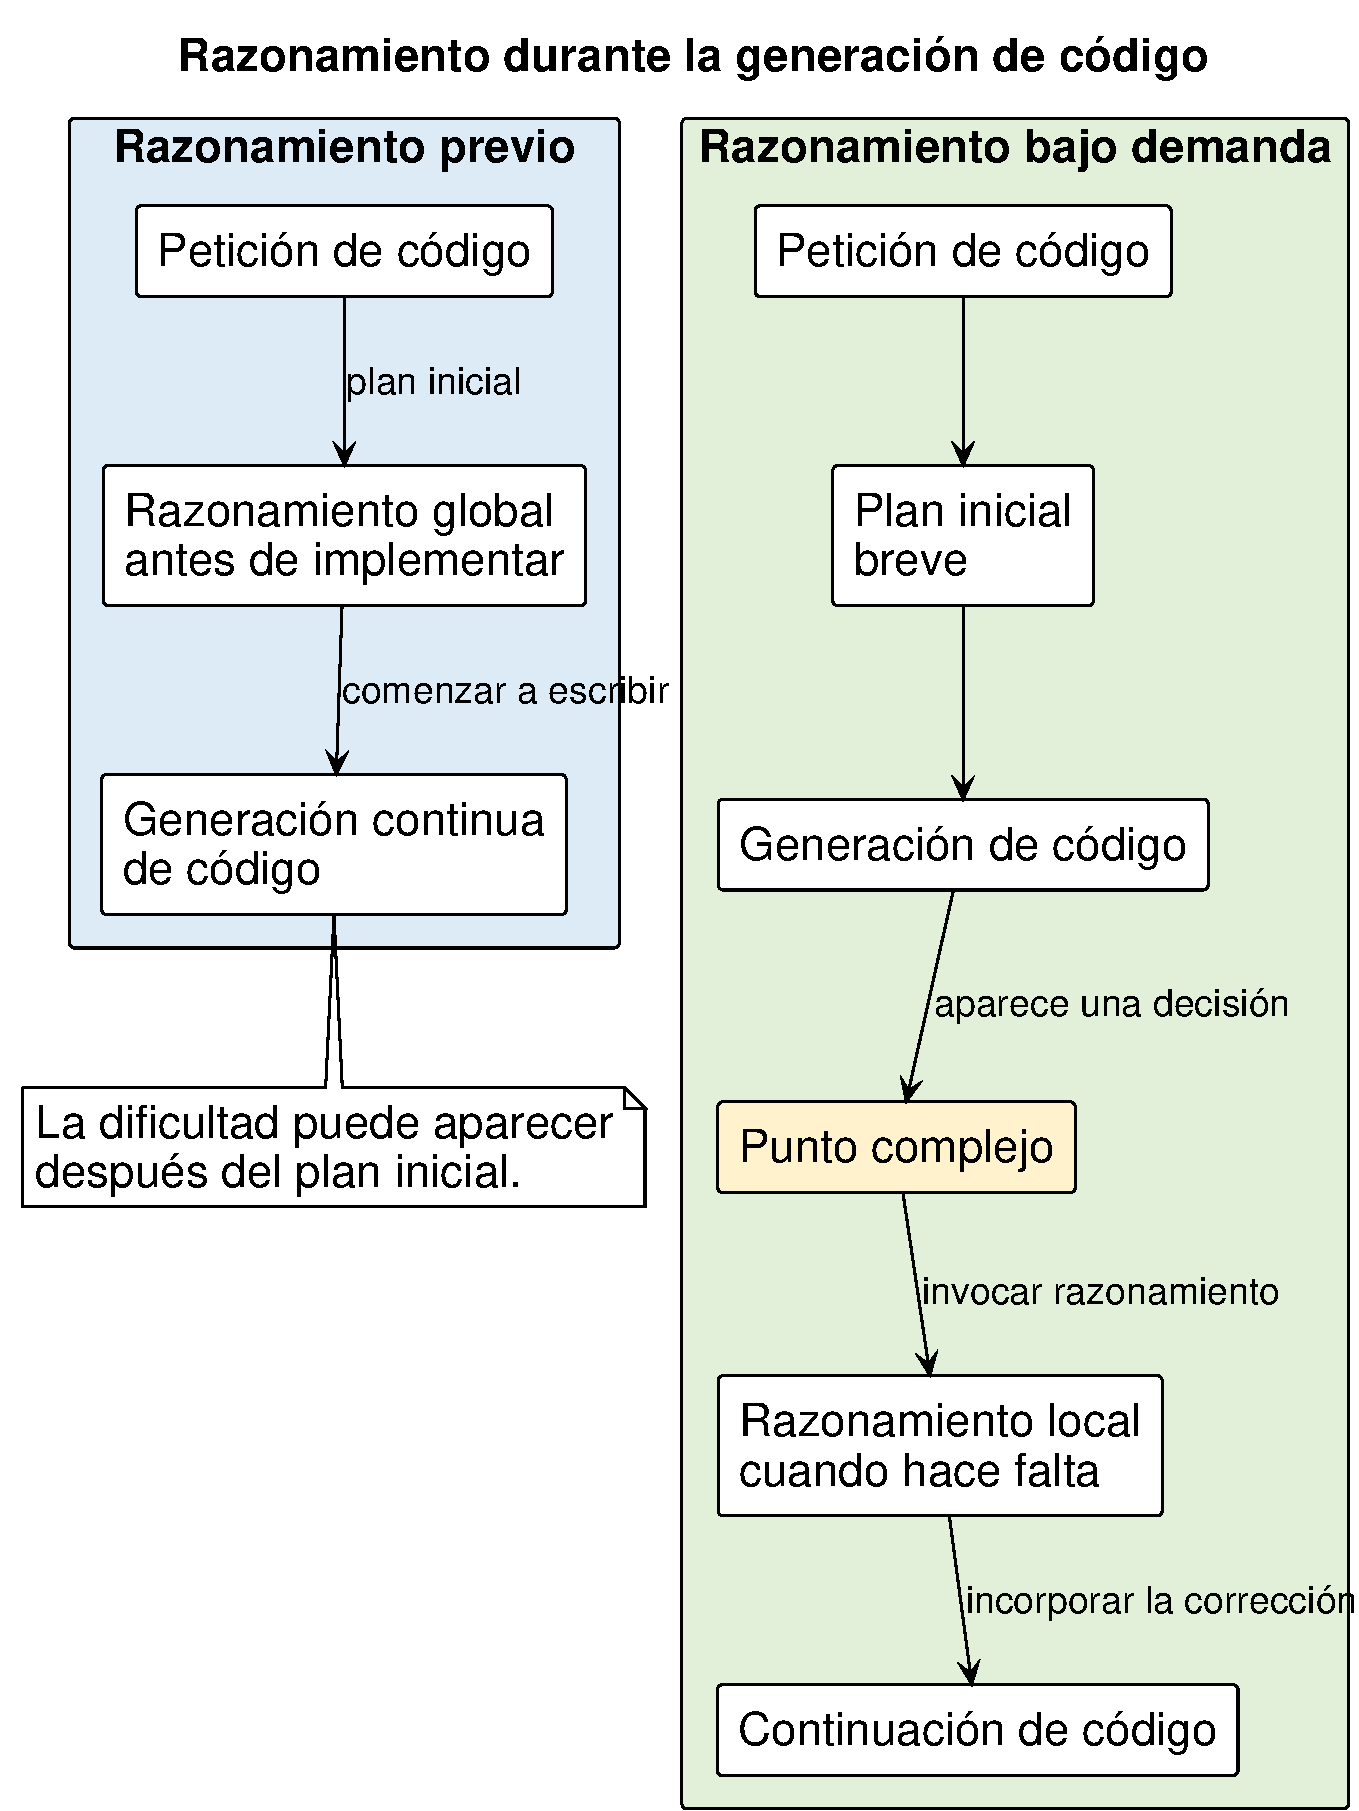
\includegraphics[width=0.48\textwidth]{figs/think-anywhere-razonamiento.pdf}\par\medskip
    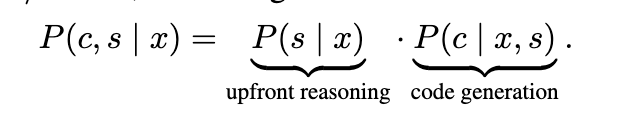
\includegraphics[width=0.65\textwidth]{figs/paper1.1.png}\par\medskip
    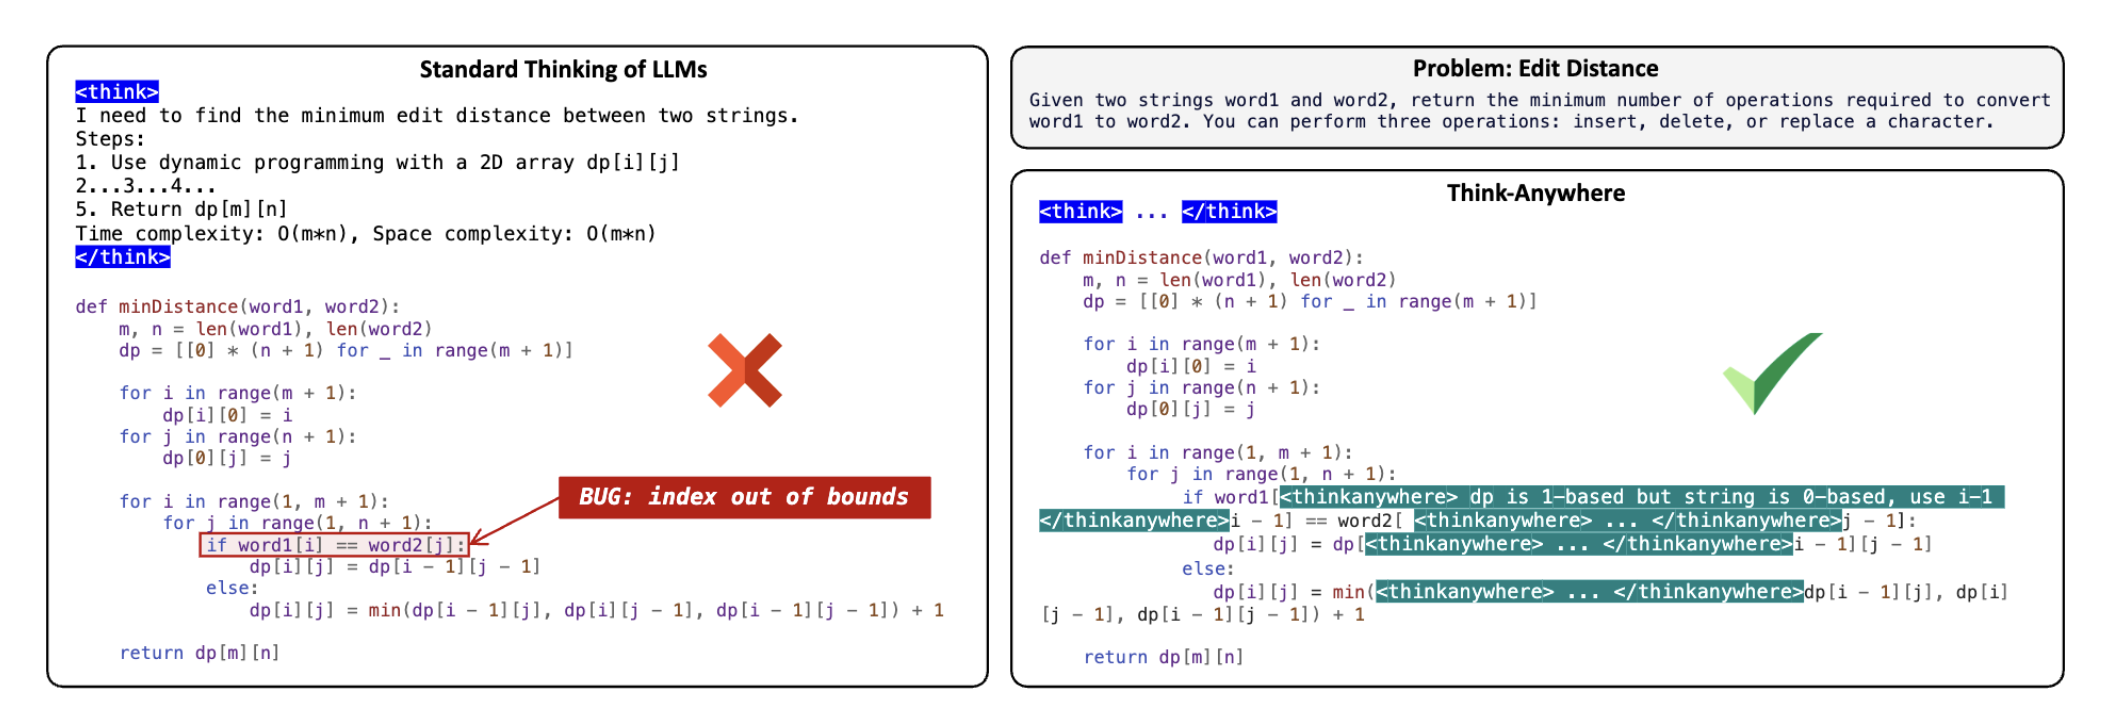
\includegraphics[width=0.92\textwidth]{figs/paper1.2.png}
    \caption[Razonamiento bajo demanda en Think-Anywhere]{Razonamiento bajo demanda en Think-Anywhere. Arriba, diagrama conceptual del artículo y abajo las capturas de la formulación y del ejemplo de generación de código de Jiang et al. \parencite[pp.~1--4]{jiang2026thinkanywhere}}
    \label{fig:think-anywhere-razonamiento}
\end{figure}

Frente a este enfoque, LocalMind-AI usa un flujo \gls{cot}-\gls{rag} guiado por instrucciones, con búsqueda en una base vectorial y herramientas expuestas por un servidor \gls{mcp}, dentro de una arquitectura local en la que el agente y el cliente web se ejecutan en contenedores separados. Think-Anywhere no persigue integrar esos componentes ni ofrecer una interfaz de usuario, por lo que su valor para LocalMind-AI está en señalar una posible evolución: decidir de forma adaptativa cuándo ampliar el razonamiento dentro de una tarea, en lugar de aplicar siempre la misma pauta de deliberación \parencite[pp.~2--6]{jiang2026thinkanywhere}.

\subsection{Google AI Edge Gallery}\label{subsec:ai-edge-gallery}

Google AI Edge Gallery es una aplicación móvil de demostración para descargar, administrar y ejecutar modelos de lenguaje en el propio dispositivo mediante \gls{litert}-LM. Permite seleccionar los backends de \gls{cpu}, \gls{gpu} o \gls{npu}, probar modelos y observar sus prestaciones desde la aplicación \cite{google2026aiedgegallery}. Además, incorpora \emph{Agent Skills}, \gls{funciontool} y soporte experimental para \gls{mcp}, de modo que las habilidades y los esquemas de herramientas se añaden al contexto de la conversación y las acciones requieren autorización del usuario \cite{google2026aiedgegallery}.

Las capturas de la Figura~\ref{fig:ai-edge-gallery-capturas} muestran la gestión de modelos, la conversación con un modelo local y la configuración de un servidor \gls{mcp}. La inferencia base se sitúa en el cliente móvil, aunque la integración de servidores remotos depende de HTTP y no permite utilizar directamente el transporte \texttt{stdio} habitual de escritorio \cite{google2026aiedgegallery}.

\begin{figure}[h!tp]
    \centering
    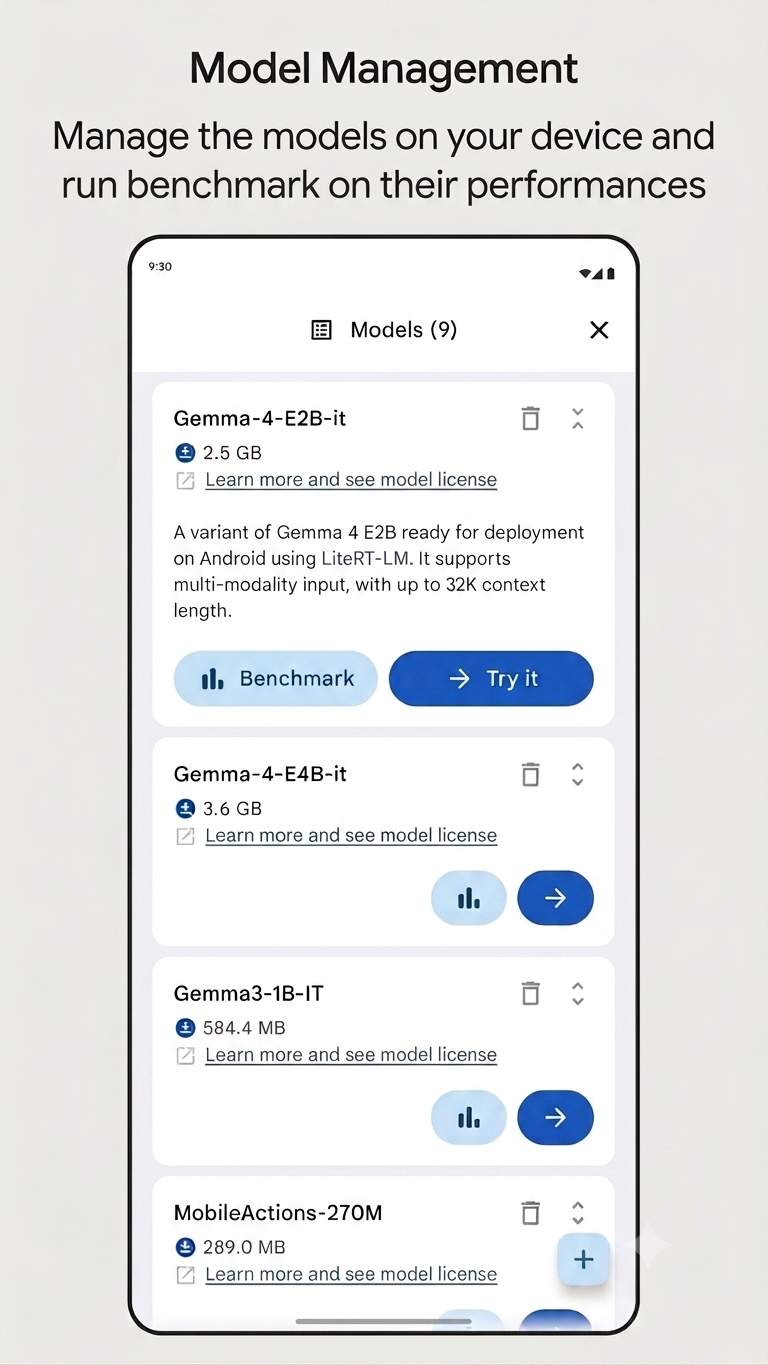
\includegraphics[height=0.35\textheight,keepaspectratio]{figs/paper2.1.png}\hfill
    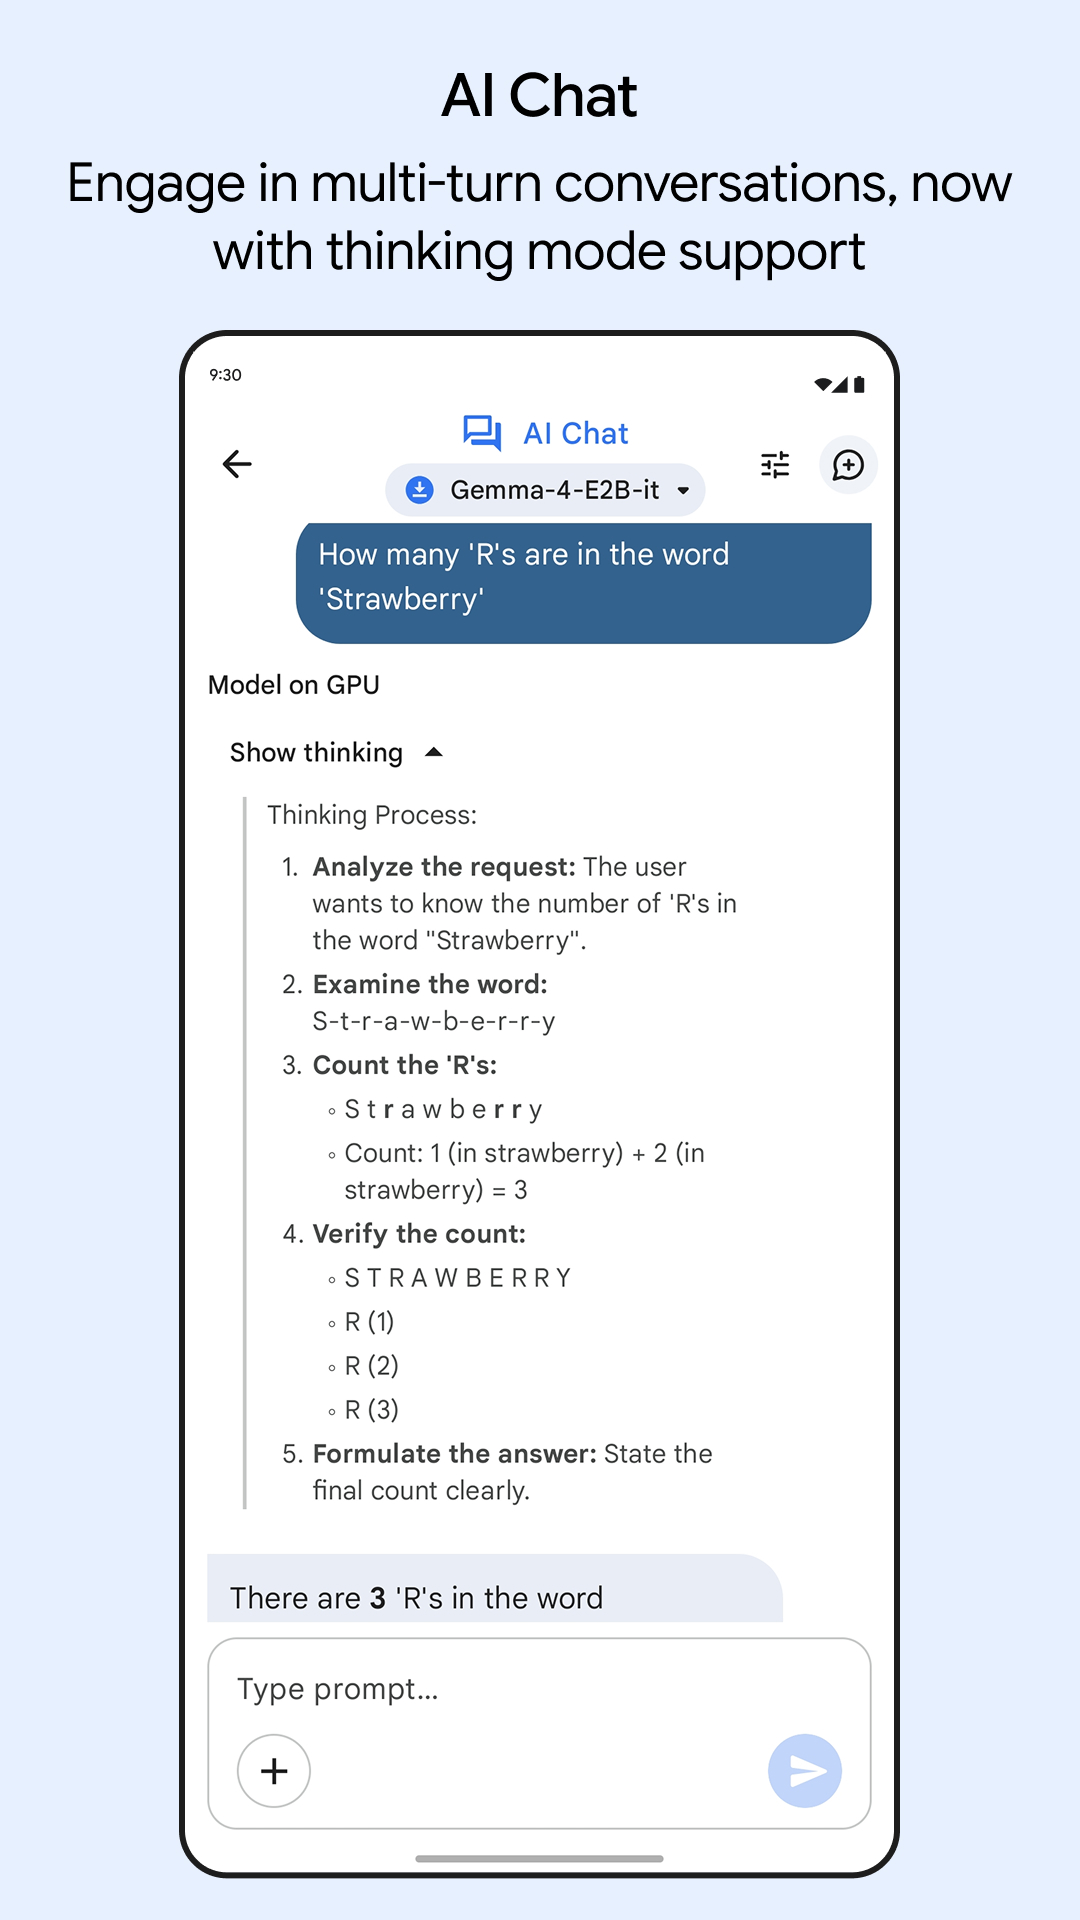
\includegraphics[height=0.35\textheight,keepaspectratio]{figs/paper2.2.jpg}\par\medskip
    
\includegraphics[height=0.33\textheight,keepaspectratio]{figs/paper2.3.png}
    \caption[Capturas de Google AI Edge Gallery]{Capturas de Google AI Edge Gallery con gestión de modelos, conversación local y administración de servidores \gls{mcp}. \cite{google2026aiedgegallery}}
    \label{fig:ai-edge-gallery-capturas}
\end{figure}

La comparación con LocalMind-AI destaca una decisión arquitectónica distinta. Edge Gallery ejecuta el modelo en el dispositivo cliente, mientras que LocalMind-AI consulta \gls{ollama} u \gls{omlx} en el anfitrión desde el contenedor del agente y entrega su aplicación \gls{reactnative} desde un segundo contenedor dedicado al cliente web. Ambos integran herramientas, pero LocalMind-AI añade un servidor \gls{mcp} propio y recuperación documental en \gls{chromadb}. Edge Gallery ofrece, por tanto, una referencia práctica sobre inferencia móvil y permisos de herramientas, mientras que LocalMind-AI prioriza la coordinación local entre modelo, recuperación y servicios.

\subsection{TinyAgent}\label{subsec:tinyagent}

TinyAgent es una demostración académica publicada en \gls{emnlp} 2024 que aborda la \gls{funciontool} en el borde mediante \glspl{agenteia} específicos de tarea. El trabajo presenta variantes de 1,1 y 7 mil millones de parámetros y utiliza \gls{llmcompiler} para obtener planes de funciones, el plan resultante expresa las dependencias entre invocaciones antes de ejecutar las herramientas \parencite[pp.~80--84]{erdogan2024tinyagent}. La contribución no consiste en una interfaz generalista, sino en articular \gls{planeacion}, selección de herramientas y ejecución para un asistente \gls{macos} con un conjunto de funciones definido \parencite[pp.~82--84]{erdogan2024tinyagent}.

Para limitar el contexto que recibe el modelo, \gls{toolrag} recupera las descripciones y los ejemplos de las herramientas pertinentes para cada solicitud. El artículo también evalúa cuantización a 4 bits como parte de su estrategia de despliegue y mide el éxito de los planes de funciones bajo las condiciones de su demostración \parencite[pp.~84--88]{erdogan2024tinyagent}. Estos resultados respaldan la discusión sobre agentes eficientes y selección de herramientas, pero están ligados a tareas, herramientas y hardware concretos, no permiten trasladar sus métricas a otros asistentes.

La Figura~\ref{fig:tinyagent-arquitectura} conserva el diagrama conceptual y añade la identificación visual del proyecto. Ambas piezas sitúan el flujo desde la petición hasta la herramienta seleccionada \parencite[pp.~80--85]{erdogan2024tinyagent}.

\begin{figure}[h!tp]
    \centering
    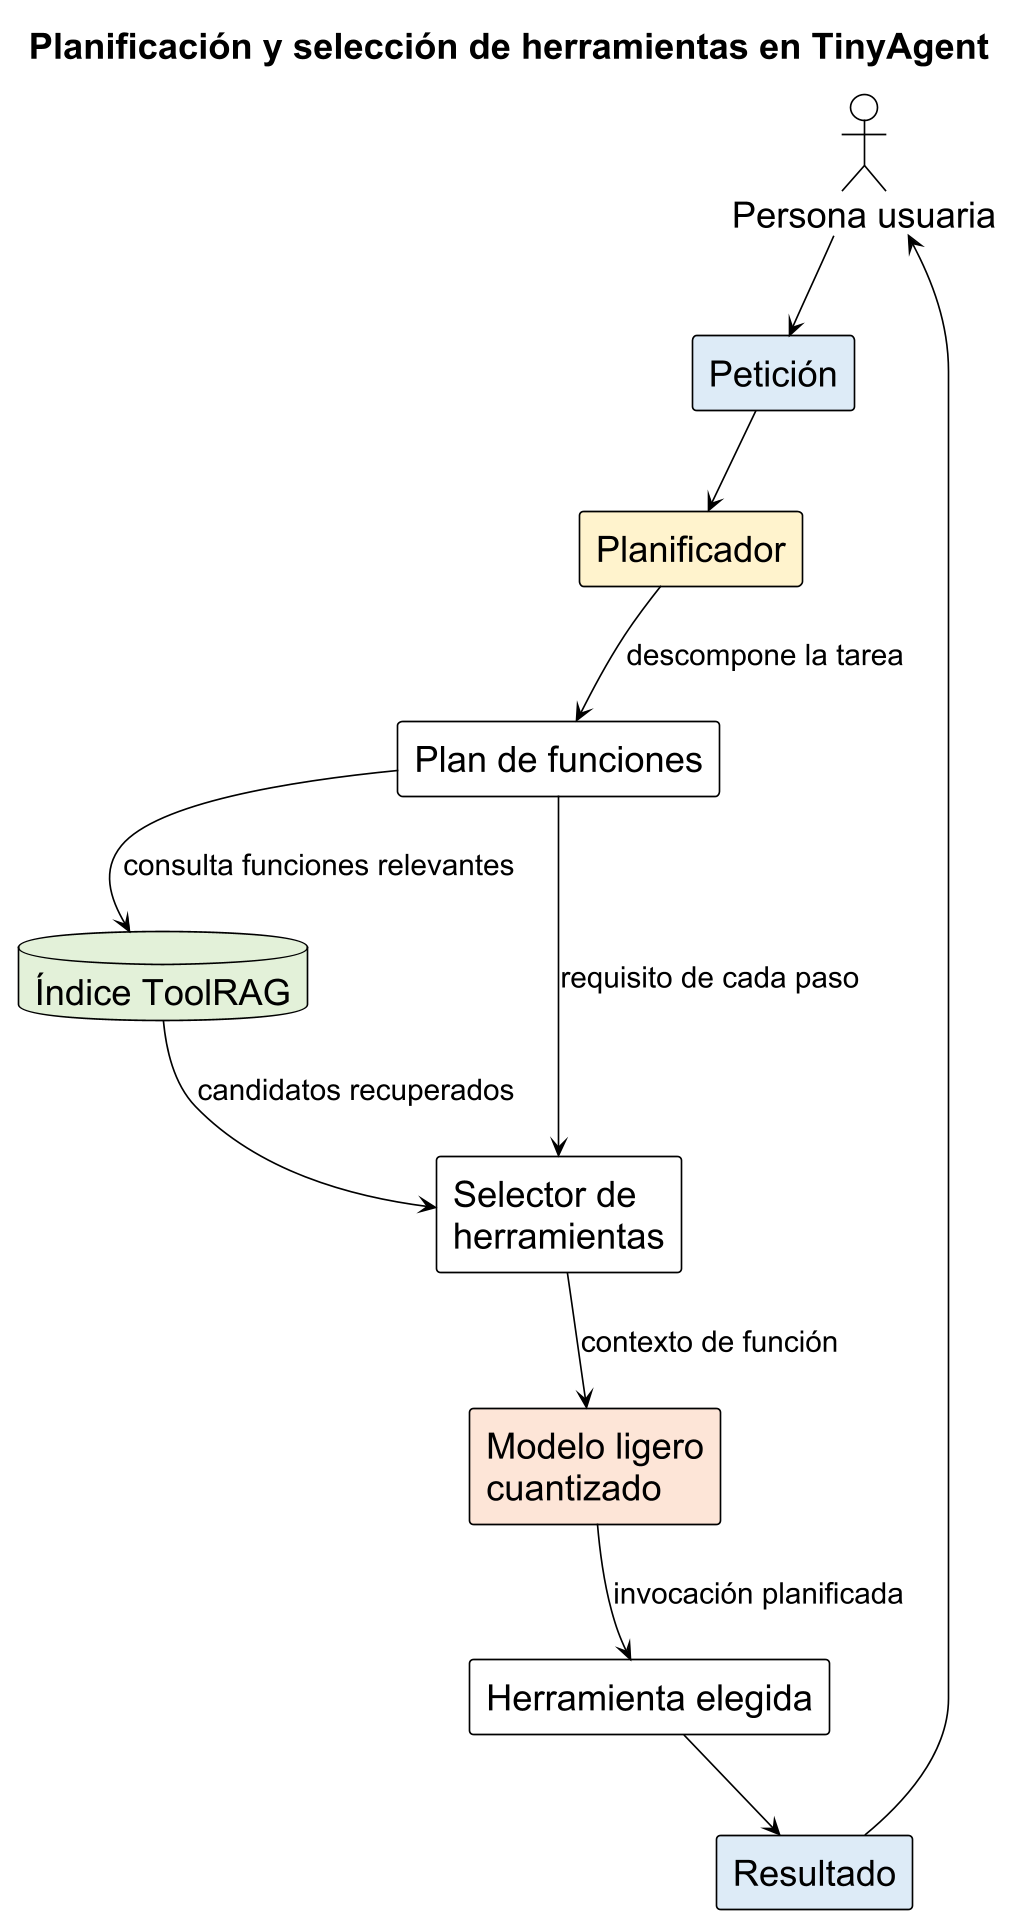
\includegraphics[width=0.46\textwidth]{figs/tinyagent-arquitectura.png}\par\medskip
    
\includegraphics[width=0.82\textwidth]{figs/paper3.1.png}
    \caption[TinyAgent y su arquitectura de planificación]{TinyAgent y su arquitectura de \gls{planeacion} y selección de herramientas. Arriba, diagrama conceptual del proyecto y abajo la identificación visual del proyecto. \parencite[pp.~80--85]{erdogan2024tinyagent}}
    \label{fig:tinyagent-arquitectura}
\end{figure}

La comparación con LocalMind-AI es parcial. TinyAgent se demuestra como asistente \gls{macos} específico de tarea y su \gls{toolrag} recupera contexto sobre herramientas, el alcance descrito no especifica integración mediante \gls{mcp} ni recuperación de una base documental general \parencite[pp.~80--88]{erdogan2024tinyagent}. Por su parte, la instantánea de LocalMind-AI documenta un flujo \gls{cot}-\gls{rag} dirigido por instrucciones, con búsqueda en \gls{chromadb}, un servidor \gls{mcp} propio y un cliente web contenido de forma independiente al agente. TinyAgent aporta así un antecedente para separar la recuperación destinada a elegir herramientas (\gls{funciontool}) de la recuperación orientada a fundamentar respuestas, sin afirmar que ambos mecanismos sean intercambiables.

\subsection{Self-RAG}\label{subsec:self-rag}

Self-RAG formula la recuperación como una decisión adaptativa durante la generación. El modelo aprende tokens de \gls{reflexion} para recuperar, generar y criticar, de forma que decide si necesita incorporar evidencia y valora la relevancia, el respaldo y la utilidad de cada resultado. Así, puede omitir la recuperación o repetirla según la evaluación interna de cada paso, frente a un flujo que recupera siempre al inicio \parencite[pp.~1--5]{asai2024selfrag}.

El artículo evalúa esta arquitectura en tareas de pregunta-respuesta, razonamiento, verificación factual y generación extensa. La Figura~\ref{fig:self-rag-captura} muestra la diferencia visual entre un flujo \gls{rag} convencional y la recuperación, generación y crítica iterativas de Self-RAG \parencite[pp.~1, 6--10]{asai2024selfrag}.

\begin{figure}[h!tp]
    \centering
    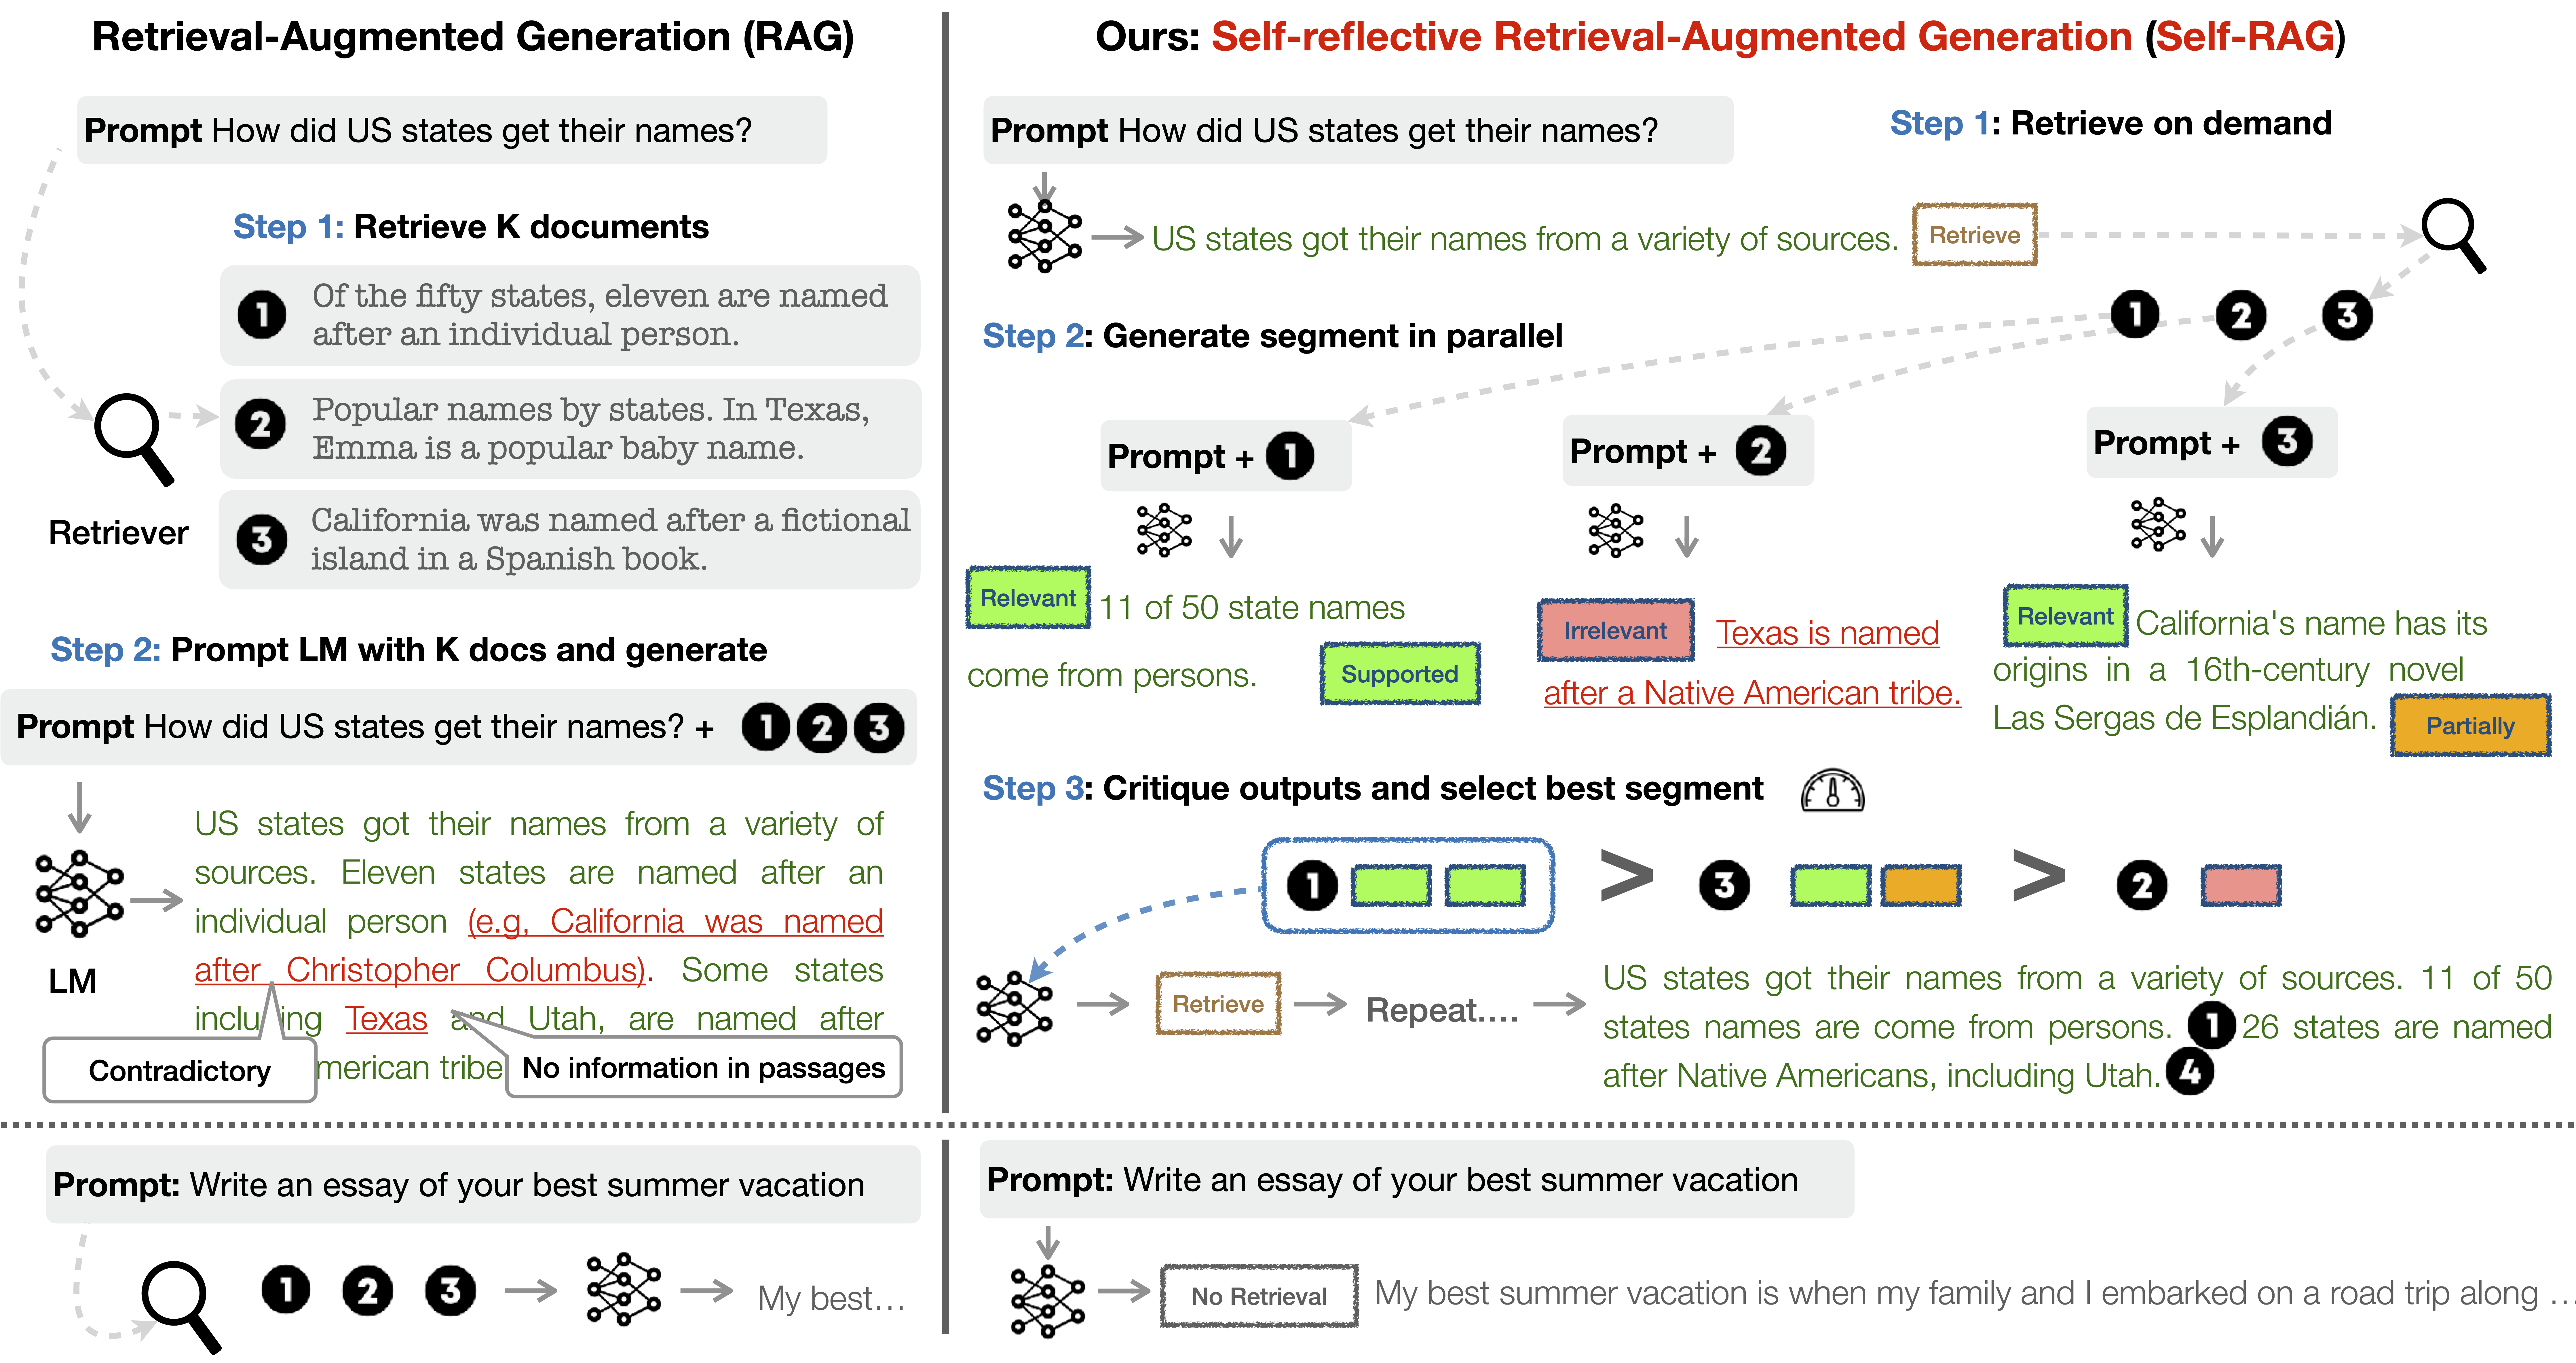
\includegraphics[width=0.95\textwidth]{figs/paper4.1.png}
    \caption[Comparación entre RAG y Self-RAG]{Comparación entre un flujo \gls{rag} convencional y la recuperación autorreflexiva de Self-RAG. \parencite[pp.~1--5]{asai2024selfrag}}
    \label{fig:self-rag-captura}
\end{figure}

La comparación con LocalMind-AI se sitúa en la coordinación entre razonamiento y recuperación. LocalMind-AI documenta un flujo \gls{cot}-\gls{rag} guiado por instrucciones, con herramientas accesibles mediante \gls{mcp} y una base \gls{chromadb}, separando además el agente y el cliente web en dos servicios contenerizados. Self-RAG integra la decisión de recuperar y la crítica en el modelo entrenado, mientras que LocalMind-AI orquesta esos componentes desde su arquitectura de aplicación. Por ello, Self-RAG sirve como referencia para valorar estrategias de recuperación adaptativa, no como una descripción de una capacidad ya implementada en LocalMind-AI \parencite[pp.~1--5]{asai2024selfrag}.

\subsection{Conclusiones}\label{subsec:conclusiones-tecnologias-similares}

Los cuatro casos examinados cubren dimensiones complementarias y no son equivalentes como productos ni como evidencia. Think-Anywhere estudia el razonamiento bajo demanda para generación de código y se mantiene en condición de \emph{preprint} sin revisión por pares \cite{jiang2026thinkanywhere}. Google AI Edge Gallery aporta evidencia oficial no académica sobre inferencia en el cliente móvil, habilidades y soporte experimental de \gls{mcp} \cite{google2026aiedgegallery}. TinyAgent demuestra \gls{planeacion} de funciones y selección de contexto de herramientas en un asistente macOS específico de tarea \cite{erdogan2024tinyagent}, Self-RAG aporta una arquitectura de investigación para decidir, recuperar, generar y criticar durante la producción de una respuesta \cite{asai2024selfrag}. Esta diversidad explica por qué una comparación controlada debe atender al alcance de cada fuente, no derivar un orden de rendimiento entre propuestas heterogéneas.

LocalMind-AI se diferencia por la combinación documentada de un modelo servido por \gls{ollama} o \gls{omlx} en un host local, un cliente \gls{reactnative}/\gls{expo} y un agente desplegados en contenedores independientes, servidores \gls{mcp} iniciados como subprocesos y recuperación sobre \gls{chromadb} dentro de un flujo \gls{cot}-\gls{rag} dirigido por instrucciones. Esa combinación permite situarlo entre los referentes anteriores sin prometer capacidades no implementadas, ya que la evidencia actual no acredita inferencia directamente en el cliente como Edge Gallery, \gls{planeacion} entrenada de funciones como TinyAgent, ni autorreflexión adaptativa entrenada como Self-RAG \cite{google2026aiedgegallery,erdogan2024tinyagent,asai2024selfrag}. Del mismo modo, Think-Anywhere informa una posible línea de razonamiento adaptativo, pero no valida el despliegue, la recuperación documental ni las herramientas de LocalMind-AI \cite{jiang2026thinkanywhere}. La aportación diferenciada del proyecto es, por tanto, la integración observada de esos componentes en un asistente de ámbito local, cuya evaluación tecnológica se desarrolla en la sección siguiente.

\section{Evaluación de tecnologías para el desarrollo del TFM}\label{sec:evaluacion-tecnologias}

La evaluación de tecnologías se organiza en tres bloques principales, correspondientes a hardware, infraestructura y software. Esta división permite analizar cada herramienta según su función real sin mezclar conceptos. El criterio central del proyecto es el enfoque \emph{local-first} de LocalMind-AI, por el que los modelos de lenguaje, la base de datos vectorial y la memoria de trabajo deben ejecutarse y almacenarse en el equipo del usuario. A continuación, se detallan las alternativas consideradas en cada apartado y se justifica la elección final.

\subsection{Hardware}\label{subsec:hardware-localmind}

\subsubsection{Ordenadores de desarrollo y validación}

Para comprobar el rendimiento del sistema se han evaluado tres portátiles con características distintas. El modelo HP OMEN actúa como referencia histórica de recursos limitados, mientras que los equipos de MSI y Apple permiten validar la solución en los dos entornos previstos, que corresponden a \gls{windows} con tarjeta gráfica dedicada NVIDIA y \gls{macos} con chips Apple Silicon.

\paragraph{OMEN by HP 15-ce033ns.}
Este equipo sirve como referencia histórica y cuenta con las siguientes especificaciones \cite{hp2017omen15ce033ns}.
\begin{itemize}[leftmargin=*,nosep]
    \item \textbf{Procesador.} Intel Core i7-7700HQ (4 núcleos, 2,8~GHz base y hasta 3,8~GHz turbo).
    \item \textbf{Memoria \gls{ram}.} 12~GB de SDRAM DDR4-2400.
    \item \textbf{Tarjeta gráfica.} NVIDIA GeForce GTX 1050 con 2~GB de \gls{vram} GDDR5 dedicada.
    \item \textbf{Almacenamiento.} Disco duro SATA de 1~TB a 7200~rpm.
    \item \textbf{Función en el proyecto.} Referencia de hardware antiguo, no se utiliza como equipo objetivo de pruebas.
\end{itemize}
Los 2~GB de \gls{vram} y la antigüedad del procesador limitan tanto el tamaño de los modelos como la ejecución simultánea del agente, la interfaz y el motor de inferencia. Por ello, se descarta para las pruebas principales.

\paragraph{MSI Pulse GL66 12UEK-085ES.}
Es un portátil de rendimiento medio-alto que venía de fábrica con 16~GB de memoria \cite{MSIPulseGL66}. Para este TFM se utiliza con la siguiente configuración.
\begin{itemize}[leftmargin=*,nosep]
    \item \textbf{Procesador.} Intel Core i7-12700H (14 núcleos, 20 hilos, de 2,3 a 4,7~GHz).
    \item \textbf{Memoria \gls{ram}.} Ampliada por el autor a 32~GB DDR4-3200 en dos módulos de 16~GB.
    \item \textbf{Tarjeta gráfica.} NVIDIA GeForce RTX 3060 con 6~GB de \gls{vram} GDDR6 dedicada.
    \item \textbf{Almacenamiento.} SSD NVMe PCIe de 1~TB.
    \item \textbf{Función en el proyecto.} Equipo principal de validación para \gls{windows} y \gls{linux}, con aceleración \gls{cuda} para la inferencia nativa y \gls{docker} para los componentes de aplicación.
\end{itemize}
La ampliación a 32~GB de \gls{ram} realizada por el autor permite ejecutar al mismo tiempo los contenedores de la aplicación y los modelos cuantizados en el anfitrión, aunque los 6~GB de \gls{vram} limitan el tamaño máximo de los modelos que se pueden cargar en la \gls{gpu}.

\paragraph{MacBook Air M4.}
Es el equipo elegido para validar el entorno \gls{macos} con Apple Silicon \cite{apple2025macbookair}.
\begin{itemize}[leftmargin=*,nosep]
    \item \textbf{Procesador.} Chip Apple M4 con \gls{cpu} de 10 núcleos.
    \item \textbf{Memoria \gls{ram}.} 16~GB de memoria unificada compartida entre \gls{cpu}, \gls{gpu} y sistema.
    \item \textbf{Aceleración hardware.} \Gls{gpu} integrada de 10 núcleos y Neural Engine de 16 núcleos mediante el entorno \gls{mlx}.
    \item \textbf{Almacenamiento.} SSD de 512~GB.
    \item \textbf{Función en el proyecto.} Redacción de la memoria y equipo de validación para \gls{macos} con \gls{omlx} y \gls{mlx}.
\end{itemize}
La arquitectura de memoria unificada evita copiar datos entre la \gls{ram} y la \gls{vram}, reduciendo la latencia. Sin embargo, al compartir esos 16~GB con el sistema operativo y el navegador, la cuantización del modelo resulta clave para no agotar la memoria.

\textbf{Decisión.} Se descarta el HP OMEN como entorno de pruebas. La validación de LocalMind-AI se realiza de forma dual en el MSI Pulse GL66 y en el MacBook Air M4, cubriendo así dos arquitecturas de aceleración muy diferentes (NVIDIA \gls{cuda} y Apple Silicon).

\subsection{Infraestructura, virtualización y despliegue}\label{subsec:contenedores-localmind}

\subsubsection{Sistemas operativos anfitriones}

LocalMind-AI está diseñado para funcionar en \gls{windows} y \gls{macos}, manteniendo compatibilidad con \gls{linux} en equipos donde estén disponibles \gls{docker}, \gls{python} y el motor de inferencia elegido. El proyecto no requiere instalar ni gestionar explícitamente \gls{wsl2}; en Windows, Docker Desktop puede abstraer internamente esta capa sin incorporarla al flujo de configuración de LocalMind-AI. De este modo, en \gls{macos} la inferencia se apoya en \gls{mlx}, mientras que en \gls{windows} o \gls{linux} se utiliza \gls{ollama} con aceleración NVIDIA \cite{ollama2024,omlx2026}.

\subsubsection{Tecnologías de gestión de contenedores}

Para la virtualización ligera se dispone de diversas alternativas con filosofías de arquitectura diferenciadas. \Gls{docker} constituye el formato estándar y el ecosistema más consolidado para definir imágenes, redes y volúmenes persistentes mediante un demonio centralizado \cite{DockerAcceleratedContainer2022}. Por su parte, \Gls{podman} ofrece una herramienta compatible con la especificación de la Open Container Initiative que opera sin demonio central (\emph{daemonless}), facilitando la ejecución en entornos restringidos o sin privilegios de administración \cite{podman2026}. Como propuesta reciente en sistemas Apple Silicon, la herramienta de código abierto \gls{containercli} de Apple (\texttt{apple/container}) proporciona una solución nativa para gestionar contenedores Linux sobre \gls{macos} utilizando directamente el marco de virtualización del sistema operativo y el hipervisor de Darwin con una huella de memoria reducida \cite{applecontainer2026}. Por último, \Gls{lxc} proporciona contenedores de sistema orientados a la virtualización completa del sistema operativo, lo que resulta más pesado y menos adecuado para aislar los microservicios discretos de LocalMind-AI \cite{lxc2026}.

En la Figura~\ref{fig:PodmanDocker} se ilustra la comparación conceptual entre la arquitectura sin demonio de Podman y el demonio central de Docker. Asimismo, en la Figura~\ref{fig:LXCDocker} se resumen las diferencias entre la virtualización de sistema propia de LXC y la virtualización de aplicación basada en Docker. Por su parte, la Figura~\ref{fig:AppleContainerDocker1} y la Figura~\ref{fig:AppleContainerDocker2} detallan la comparación estructural y de flujo de ejecución entre el entorno nativo de Apple Container CLI y la arquitectura convencional de Docker.

\begin{figure}[h!tp]
    \centering
    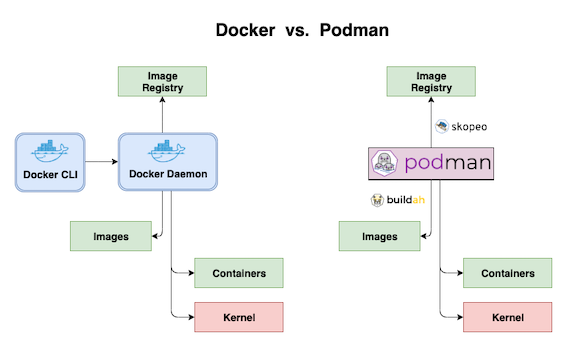
\includegraphics[width=0.78\textwidth]{figs/PodmanDocker.png}
    \caption{Comparación conceptual entre las arquitecturas de Podman y Docker.}
    \label{fig:PodmanDocker}
\end{figure}

\begin{figure}[h!tp]
    \centering
    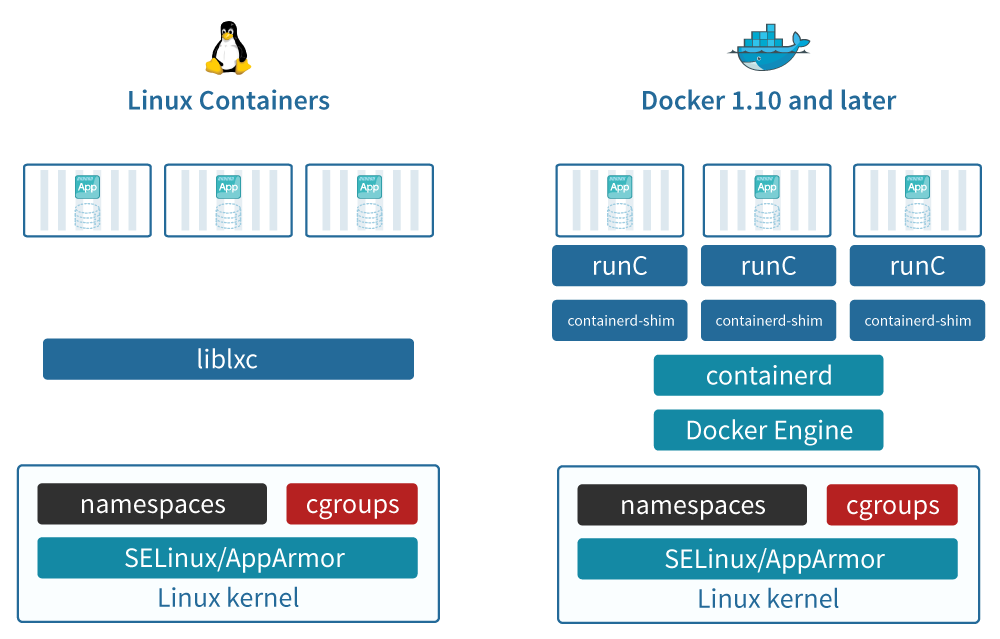
\includegraphics[width=0.78\textwidth]{figs/LXCDocker.png}
    \caption{Comparación conceptual entre los contenedores de sistema LXC y los contenedores de aplicación Docker.}
    \label{fig:LXCDocker}
\end{figure}

\begin{figure}[h!tp]
    \centering
    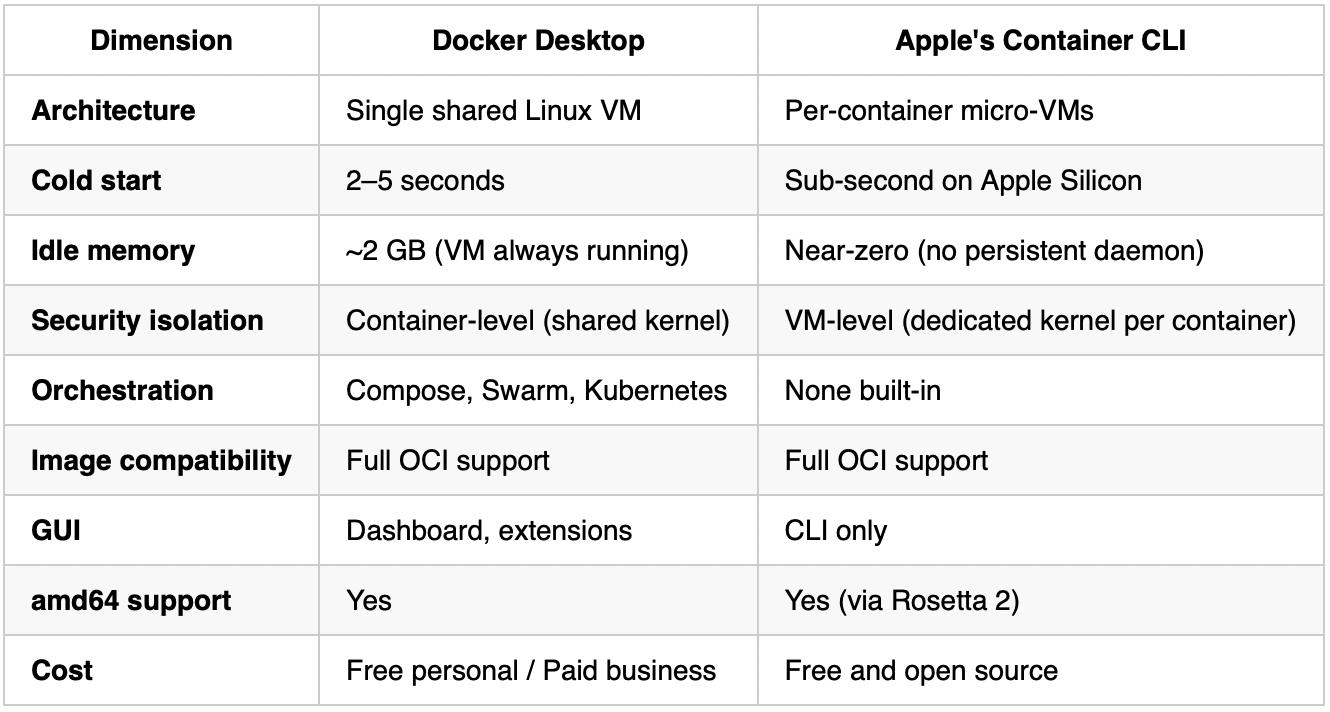
\includegraphics[width=0.78\textwidth]{figs/comp_containerVSdocker1.jpeg}
    \caption{Comparación estructural entre la arquitectura nativa de Apple Container CLI y Docker.}
    \label{fig:AppleContainerDocker1}
\end{figure}

\begin{figure}[h!tp]
    \centering
    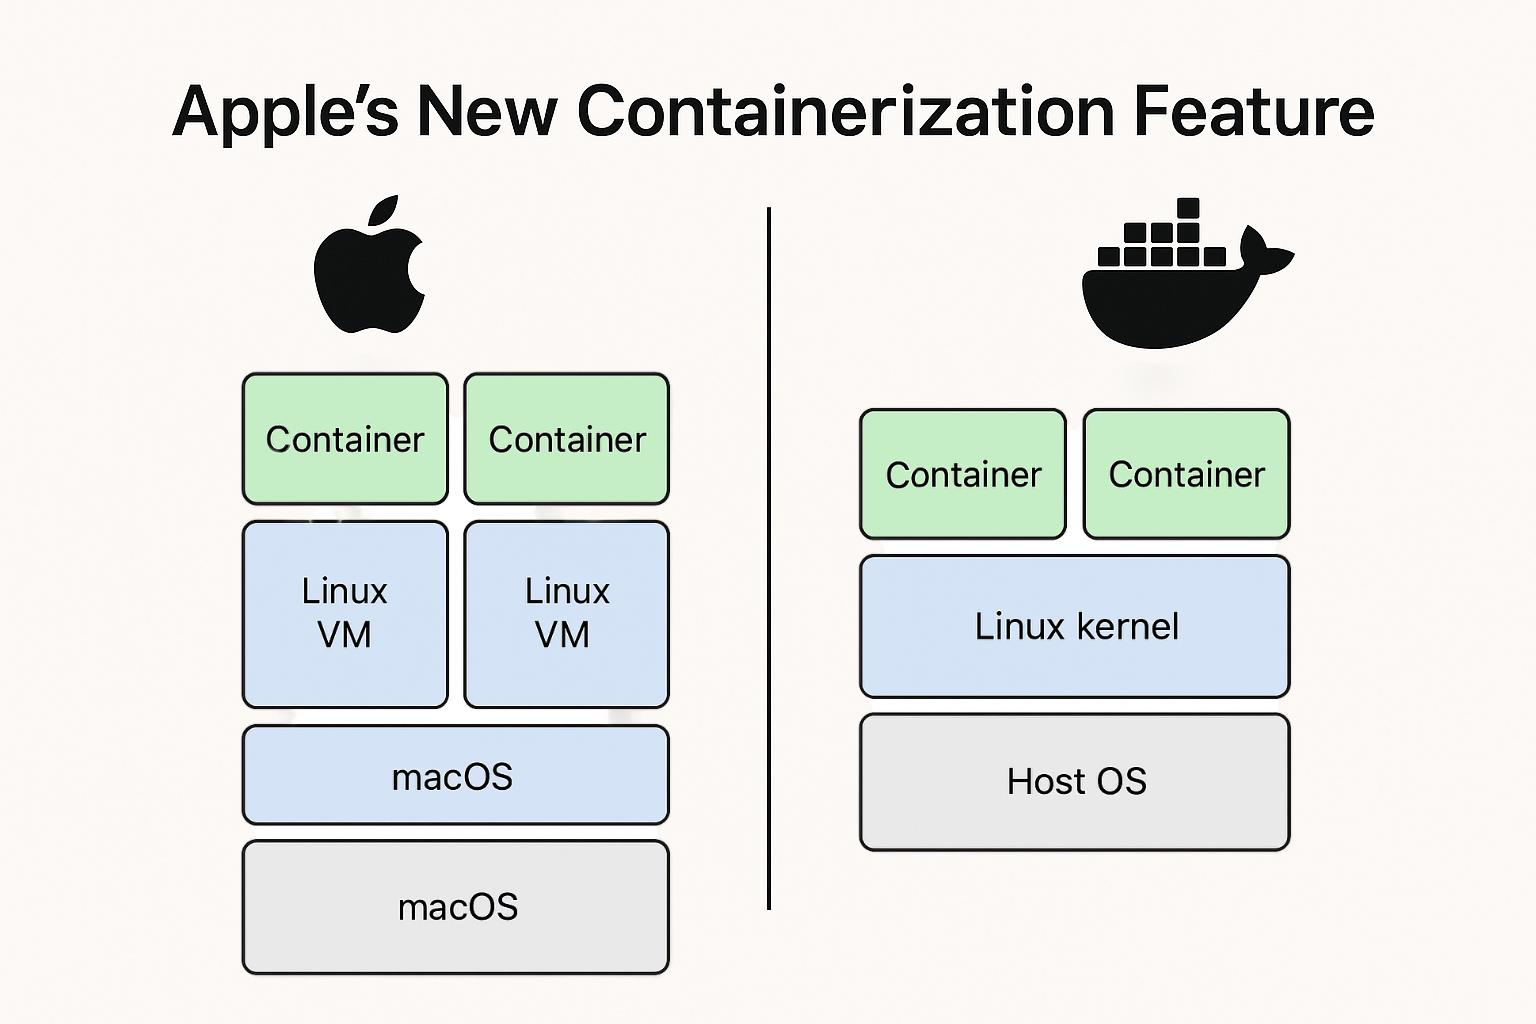
\includegraphics[width=0.78\textwidth]{figs/comp_containerVSdocker2.jpeg}
    \caption{Comparación de flujo de ejecución entre Apple Container CLI y la infraestructura de Docker.}
    \label{fig:AppleContainerDocker2}
\end{figure}

\textbf{Decisión.} Se adopta \gls{docker} como motor de ejecución principal debido a su soporte multiplataforma garantizado en \gls{windows}, \gls{macos} y \gls{linux}, su ecosistema de orquestación y su capacidad para ofrecer un entorno de validación reproducible. Las herramientas Podman y \gls{containercli} de Apple representan alternativas válidas y prometedoras para entornos sin demonio o específicos de \gls{macos}, si bien la solución basada en Docker permite mantener una especificación unificada sin introducir dependencias exclusivas de una plataforma concreta.

\subsubsection{Orquestación del despliegue con Docker Compose}

Desplegar manualmente los contenedores exige gestionar a mano los puertos, los volúmenes de datos y las variables de entorno de cada servicio. \Gls{dockercompose} simplifica este proceso definiendo toda la infraestructura en un archivo \gls{yaml}, lo que permite arrancar el sistema completo con un solo comando \cite{docker2024compose}. Herramientas como \gls{kubernetes} o \gls{minikube} permiten orquestar clústeres complejos, pero su gestión de réplicas y alta disponibilidad resulta excesiva para un asistente local orientado a un solo usuario.

La configuración de Compose contiene dos servicios de aplicación. El servicio \texttt{nanobot} aloja el agente, la pasarela \gls{websocket}, la \gls{api} \gls{rest} y los servidores de herramientas \gls{mcp}, incluido \gls{engram}, que se inician como subprocesos y no como contenedores independientes. Su imagen se construye en varias etapas y utiliza una base Python reducida para la ejecución con un usuario sin privilegios \cite{docker2026multistage}. El servicio \texttt{frontend}, por su parte, exporta el cliente \gls{expo} durante una etapa con \gls{nodejs} y \gls{pnpm}, y emplea una imagen final ligera de \gls{nginx} para servir los activos estáticos \cite{nginx2026}. Los volúmenes de \gls{docker} se destinan a los datos persistentes del agente. Por otro lado, los motores de inferencia (\Gls{ollama} u \gls{omlx}) se ejecutan fuera de \gls{docker}, directamente en el sistema anfitrión, para conservar el acceso nativo a la aceleración disponible.

\textbf{Decisión.} Se adopta \gls{dockercompose} para coordinar los servicios \texttt{nanobot} y \texttt{frontend}, manteniendo la inferencia en el anfitrión y \gls{mcp}/\gls{engram} como subprocesos del agente. Esta estructura separa la entrega del cliente web de la ejecución del agente sin añadir un contenedor por cada herramienta.

\subsection{Software}\label{subsec:software-localmind}

\subsubsection{Lenguajes de programación}

La Tabla~\ref{tab:lenguajes-software-localmind} muestra la relación entre los lenguajes utilizados y los distintos componentes del sistema.

\begin{table}[h!tp]
    \centering
    \small
    \begin{tabularx}{\textwidth}{|>{\raggedright\arraybackslash}p{4.2cm}|>{\raggedright\arraybackslash}X|}
        \hline
        \textbf{Lenguajes de programación y de marcas} & \textbf{Software o finalidad}                                                      \\
        \hline
        \gls{python}                                   & TUI, Nanobot, API con \gls{aiohttp} y servidores de herramientas MCP.              \\
        \hline
        \gls{javascript}                               & Cliente Expo/React Native Web, los archivos activos tienen extensión \texttt{.js}. \\
        \hline
        \gls{bash} y Shell                             & Instalación, detección del sistema y scripts auxiliares de control.                \\
        \hline
        \gls{yaml}                                     & Definición declarativa de Docker Compose.                                          \\
        \hline
        \gls{latex}                                    & Redacción, composición y generación de la memoria.                                 \\
        \hline
        \gls{plantuml}                                 & Diagramas de diseño y diagrama de Gantt.                                           \\
        \hline
    \end{tabularx}
    \caption{Lenguajes empleados y componentes asociados en LocalMind-AI.}
    \label{tab:lenguajes-software-localmind}
\end{table}

\Gls{python} es el lenguaje principal para la interfaz de terminal (\gls{tui}), el agente y la integración de herramientas, gracias a su amplio soporte en proyectos de inteligencia artificial y a sus bibliotecas para gestionar la terminal \cite{WelcomePythonorg2025,pythontermios2026}. \Gls{javascript} se utiliza en el cliente web porque es el lenguaje nativo de \gls{expo} y \gls{reactnative} Web \cite{expo2024,meta2024reactnative}. Por su parte, \gls{yaml} y Shell se emplean para definir el despliegue y automatizar scripts en la terminal. Finalmente, \gls{latex} y \gls{plantuml} se utilizan únicamente para la redacción de la memoria y la creación de diagramas.

\textbf{Decisión.} \Gls{python} es el lenguaje principal del agente y de la \gls{tui}, mientras que \gls{javascript} se utiliza en el cliente web.

\subsubsection{Cliente web}\label{subsec:cliente-web-localmind}

Para el desarrollo de la interfaz de usuario se evaluaron diferentes opciones. \Gls{django} ofrece un entorno completo en \gls{python} con plantillas y gestión de base de datos \cite{Django}, pero no está pensado para construir aplicaciones web dinámicas en el lado del cliente. \Gls{reactjs} permite crear interfaces basadas en componentes para aplicaciones web SPA \cite{react2026}. \Gls{angular} incluye enrutamiento y compilación bajo una estructura estricta en \gls{typescript}, idónea para grandes proyectos pero más pesada para este prototipo \cite{angular2026}. En este escenario, \gls{reactnative} Web adapta los componentes de \gls{reactnative} al navegador, y \gls{expo} facilita el empaquetado y la configuración multiplataforma \cite{meta2024reactnative,expo2024}.

\textbf{Decisión.} Se utiliza \gls{reactnative} Web con \gls{expo}. El cliente es una aplicación web escrita en \gls{javascript}, exportada como activos estáticos durante una etapa de construcción con \gls{nodejs} y \gls{pnpm}. La imagen final utiliza \gls{nginx} únicamente para servir la aplicación web, sin actuar como proxy inverso de las conexiones con el agente \cite{docker2026multistage,nginx2026}. Esta base permite reutilizar componentes en el futuro si se desarrollara una versión móvil, sin significar que dicha app móvil exista actualmente.

En el desarrollo del agente se analizaron varias alternativas. \Gls{nanobot} es un agente ligero que incluye soporte para herramientas, sesiones, memoria e integración con el protocolo \gls{mcp}, además de permitir su comunicación por red \cite{nanobot2026}. \Gls{openclaw} abarca funciones de automatización multicanal que añaden una complejidad innecesaria para este proyecto local \cite{openclaw2026}. La biblioteca \Gls{smolagents} facilita crear prototipos sencillos con herramientas, pero obligaría a programar desde cero el servidor, la gestión de sesiones y la \gls{api} \cite{smolagents2026}. Por último, \Gls{picodingagent} está diseñado específicamente para asistencia en código, por lo que no encaja como asistente general \cite{picodingagent2026}.

\textbf{Decisión.} Se adopta \gls{nanobot} como núcleo del agente por ofrecer las funciones necesarias con un consumo de recursos reducido, evitando la sobrecarga de plataformas más complejas o tener que construir la infraestructura desde cero. En la Figura~\ref{fig:NanobotArch} se ilustra el esquema conceptual de la arquitectura de Nanobot.

\begin{figure}[h!tp]
    \centering
    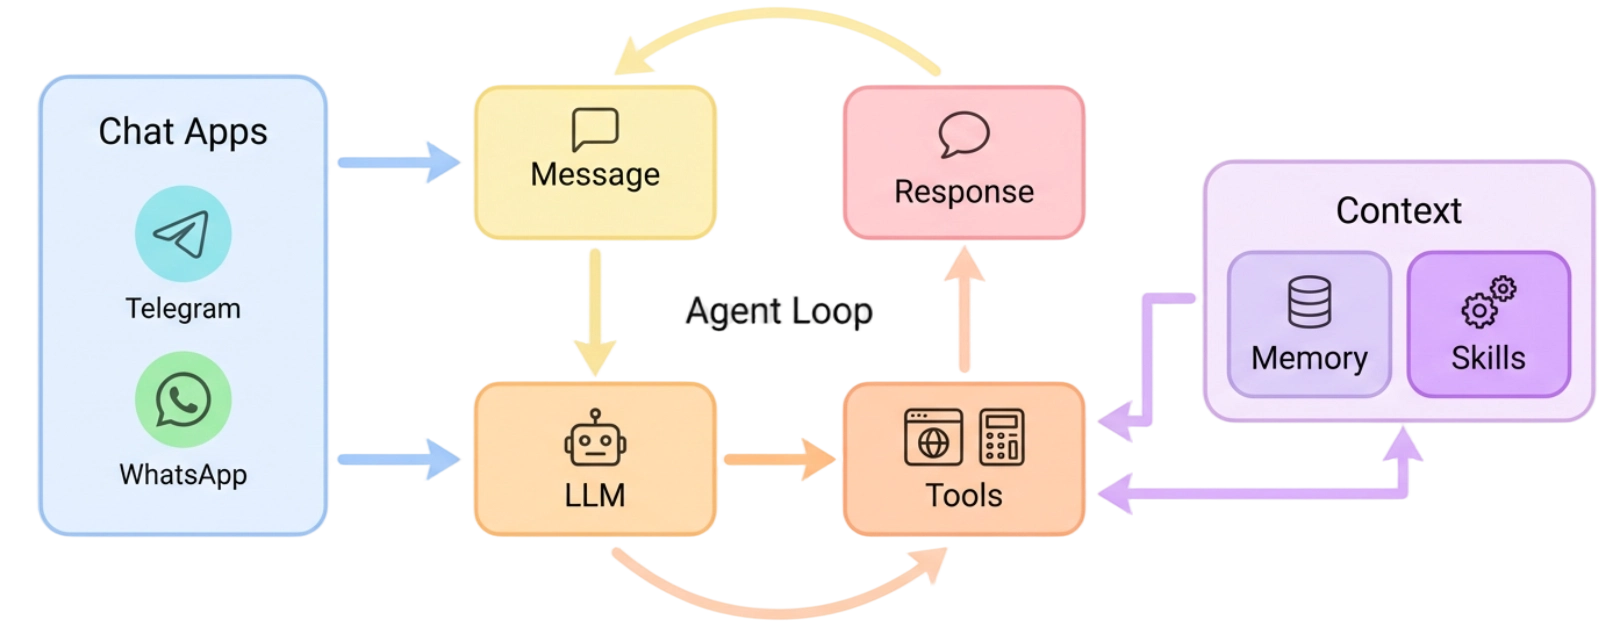
\includegraphics[width=0.85\textwidth]{figs/nanobot_arch.png}
    \caption{Esquema conceptual de la arquitectura del framework Nanobot.}
    \label{fig:NanobotArch}
\end{figure}

\subsubsection{API y comunicación}\label{subsec:agente-api-localmind}

El servidor de \gls{api} se evaluó de forma independiente al agente. Dentro del ecosistema de \gls{python}, Django REST Framework añade serialización y autenticación sobre \gls{django}, \Gls{fastapi} ofrece validación automática de datos con esquemas OpenAPI, y \Gls{flask} permite crear servicios mínimos \cite{djangorest2026,FastAPI,WelcomeFlaskFlask}. Sin embargo, la biblioteca \Gls{aiohttp} proporciona soporte asíncrono tanto para HTTP como para \gls{websocket} en un único bucle de eventos \cite{aiohttp2026}.

En cuanto a los protocolos, \Gls{websocket} permite mantener una conexión bidireccional continua, necesaria para transmitir en tiempo real (\emph{streaming}) las respuestas del modelo. Por su parte, el protocolo \Gls{rest} es idóneo para peticiones independientes y puntuales \cite{rfc6455,QueEsAPI}.

\textbf{Decisión.} Se utiliza \gls{aiohttp} para implementar el servidor. \Gls{websocket} es el canal principal para la respuesta en tiempo real, mientras que la \gls{api} \gls{rest} atiende las peticiones independientes. De este modo se aclara que el servidor no utiliza \gls{fastapi}.

\subsubsection{Instalador y configurador TUI}

La interfaz en terminal (\gls{tui}) de LocalMind guía al usuario en la detección del sistema, la elección del motor de inferencia, el modelo y las herramientas \gls{mcp}. Para su diseño se estudió como referencia el proyecto Gentle-AI, desarrollado en \gls{golang} con la biblioteca Bubble Tea y el patrón \gls{mvu} \cite{gentleai2026,bubbletea2026}, del que se tomaron ideas para la distribución visual, el uso del teclado y la navegación por pantallas.

\textbf{Decisión.} Se mantiene la \gls{tui} desarrollada en \gls{python} y se cita Gentle-AI como referencia de diseño e interfaz, sin que constituya una dependencia del código.

En la Figura~\ref{fig:TUIComparativa} se presenta la comparación visual entre la interfaz de terminal de Gentle-AI, en la Figura~\ref{fig:TUIGentle}, y la pantalla equivalente desarrollada en \gls{python} para LocalMind-AI, en la Figura~\ref{fig:TUILocalMind}.

\begin{figure}[h!tp]
    \centering
    \begin{subfigure}[b]{0.48\textwidth}
        \centering
        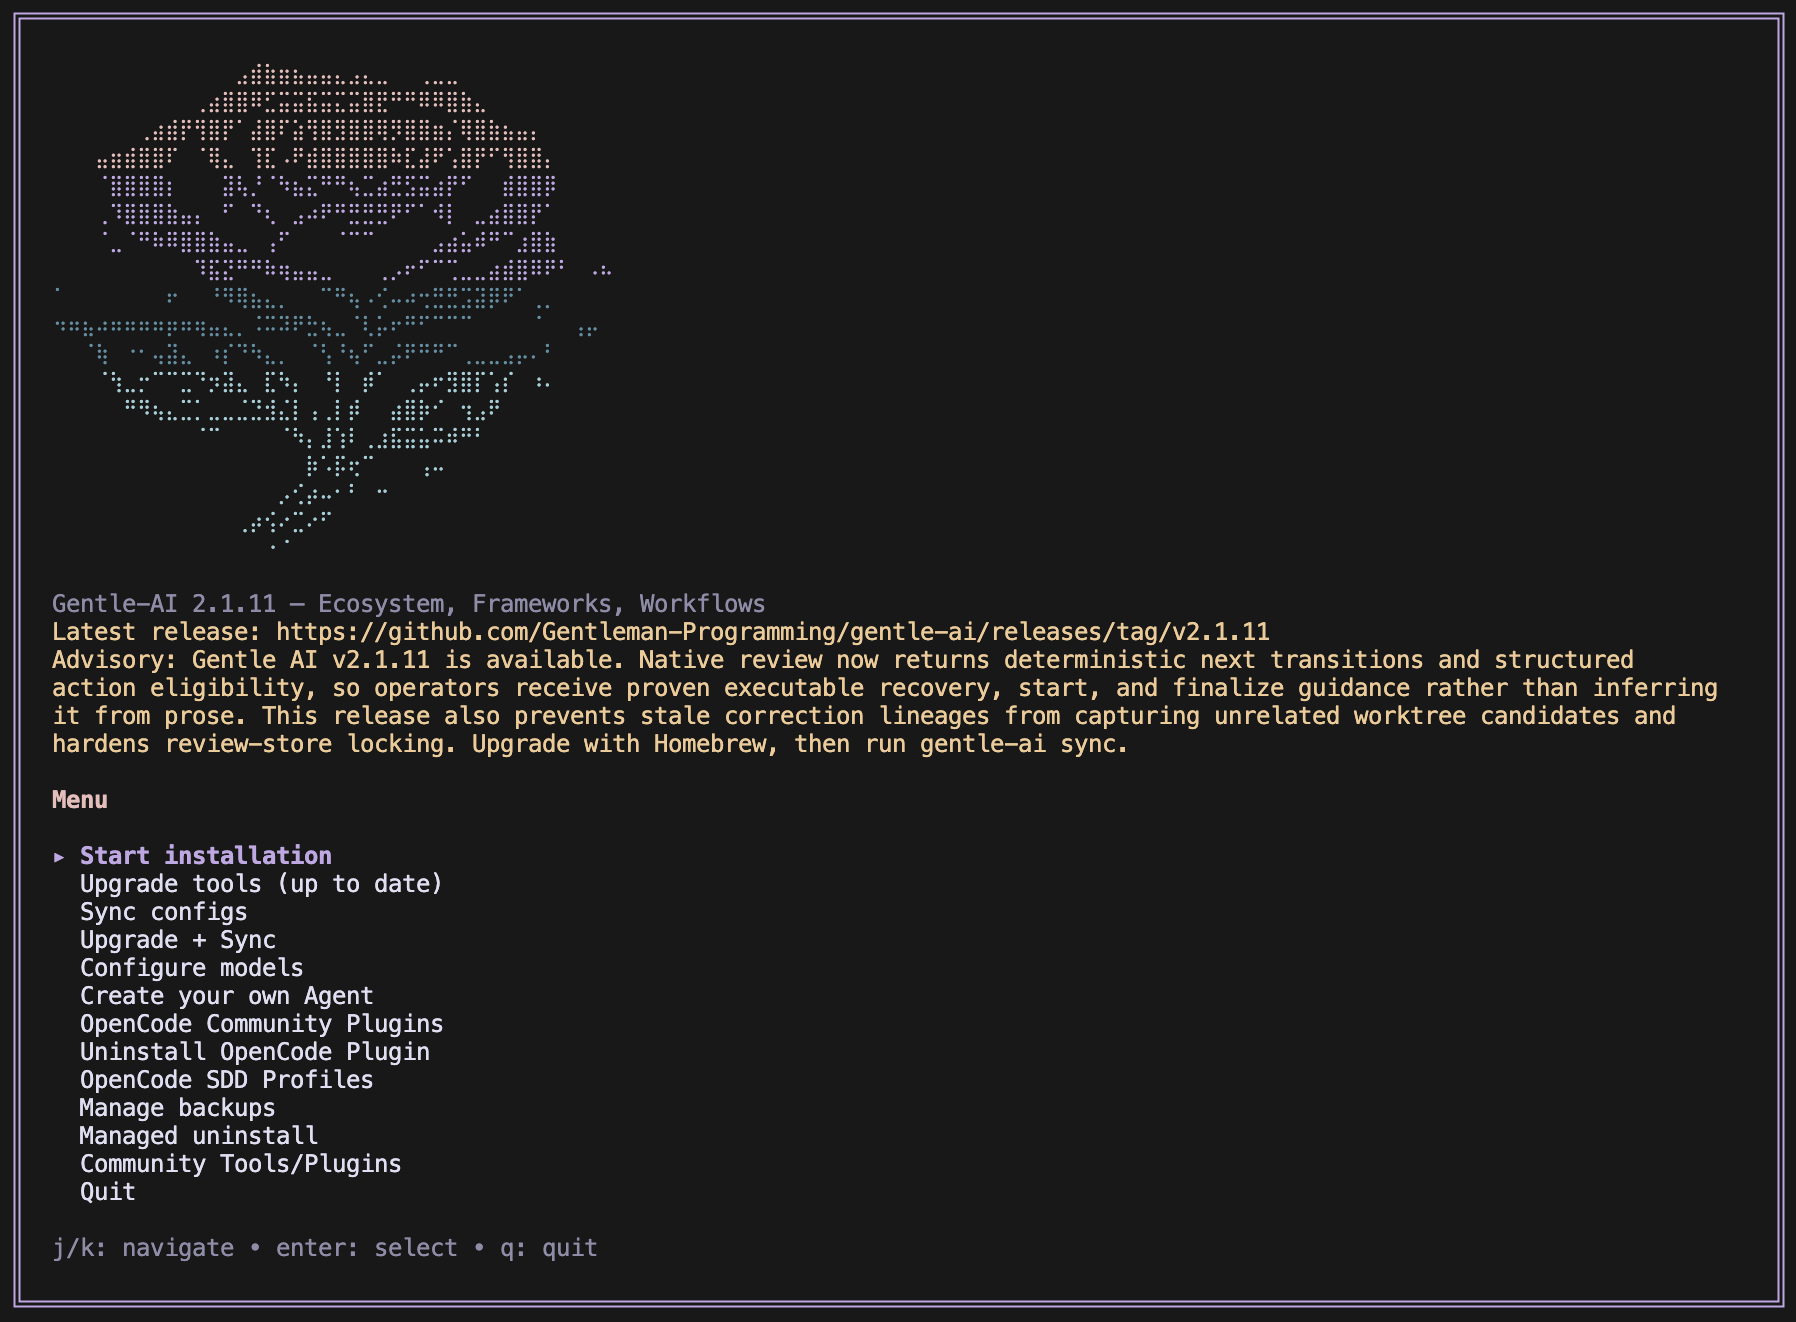
\includegraphics[width=\textwidth]{figs/tui_gentle-ai.png}
        \caption{Interfaz TUI de Gentle-AI en Golang \cite{gentleai2026}.}
        \label{fig:TUIGentle}
    \end{subfigure}
    \hfill
    \begin{subfigure}[b]{0.48\textwidth}
        \centering
        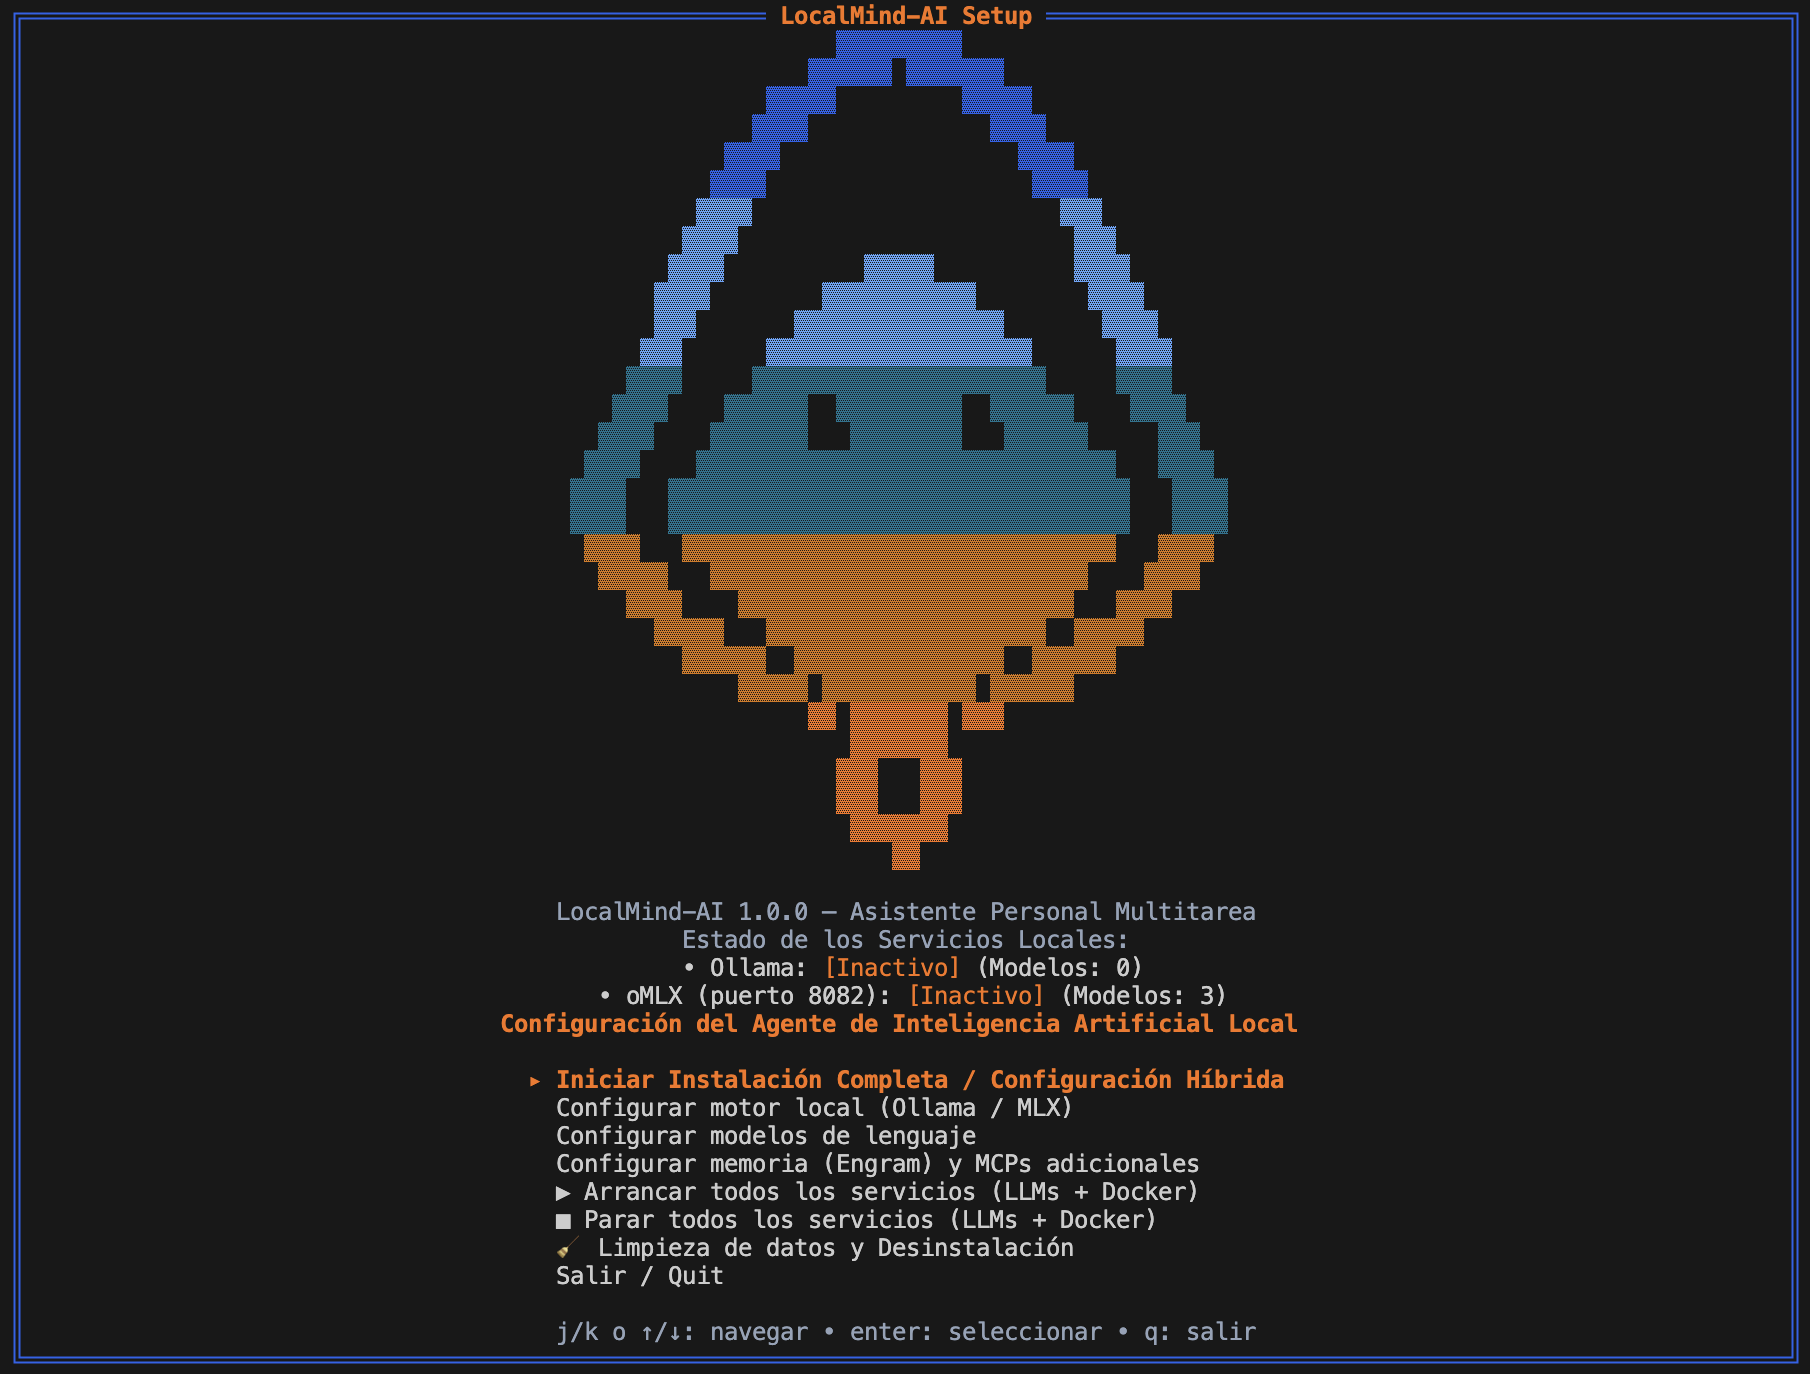
\includegraphics[width=\textwidth]{figs/tui_localmind-ai.png}
        \caption{Interfaz TUI de LocalMind-AI en Python.}
        \label{fig:TUILocalMind}
    \end{subfigure}
    \caption{Comparación visual entre la interfaz de terminal de Gentle-AI y la TUI de LocalMind-AI.}
    \label{fig:TUIComparativa}
\end{figure}

\subsubsection{Software de inferencia local}\label{subsec:inferencia-local-localmind}

Para la inferencia local se evaluaron varios motores. \Gls{ollama} simplifica la descarga y el uso de modelos mediante una \gls{api} local sencilla y está disponible en varios sistemas \cite{ollama2024}. El servidor \Gls{omlx} ofrece una \gls{api} compatible con OpenAI sobre \gls{mlx}, optimizada para Apple Silicon en \gls{macos} \cite{omlx2026}. El motor \Gls{vllm} está enfocado al alto rendimiento y procesamiento por lotes en servidores con muchos usuarios, unas ventajas poco relevantes para un asistente local individual \cite{vllm2026}. Por último, \Gls{chatrtx} combina inferencia y recuperación en \gls{windows} con tarjetas RTX, pero limita el sistema al ecosistema de NVIDIA \cite{nvidia2026chatrtx}.

\textbf{Decisión.} Se utiliza \gls{ollama} como motor general y \gls{omlx}/\gls{mlx} para entornos \gls{macos} con Apple Silicon. Ambos se ejecutan en el sistema anfitrión fuera de \gls{docker} para aprovechar la aceleración por \gls{hardware}.

\subsubsection{Modelos de IA generativa}

El sistema ofrece dos familias principales de modelos de 9.000 millones de parámetros, que son Ornith~1.0~9B y Qwen~3.5~9B, disponibles en versiones cuantizadas de 4 y 6 bits \cite{ornith9b4,ornith9b6,qwen359b}. La cuantización a 4 bits reduce el consumo de memoria y deja más recursos libres para el sistema, a costa de una pequeña pérdida de precisión. La de 6 bits conserva mejor la información de los pesos, pero requiere más \gls{ram} o \gls{vram}. La cuantización cambia la forma de representar los pesos, pero no altera el número de parámetros del modelo.

\textbf{Decisión.} La configuración recomendada en \gls{macos} es Ornith~1.0~9B cuantizado a 4 bits. Esta elección se documenta como la opción activa en las pruebas, si bien el usuario puede elegir entre Ornith/Qwen y cuantización de 4/6 bits según la memoria de su equipo.

En la Figura~\ref{fig:TUISelectorModelos} se ilustran las pantallas del instalador TUI de LocalMind-AI. La Figura~\ref{fig:TUITiposModelos} muestra la clasificación inicial de perfiles organizada en función del nivel de inteligencia y capacidad del modelo, mientras que la Figura~\ref{fig:TUIModelosCuantizacion} expone el catálogo de modelos específicos junto con la descripción comentada al lado de cada opción, la cual detalla la velocidad de respuesta esperada y el nivel de inteligencia estimado según los recursos disponibles del sistema.

\begin{figure}[h!tp]
    \centering
    \begin{subfigure}[b]{0.48\textwidth}
        \centering
        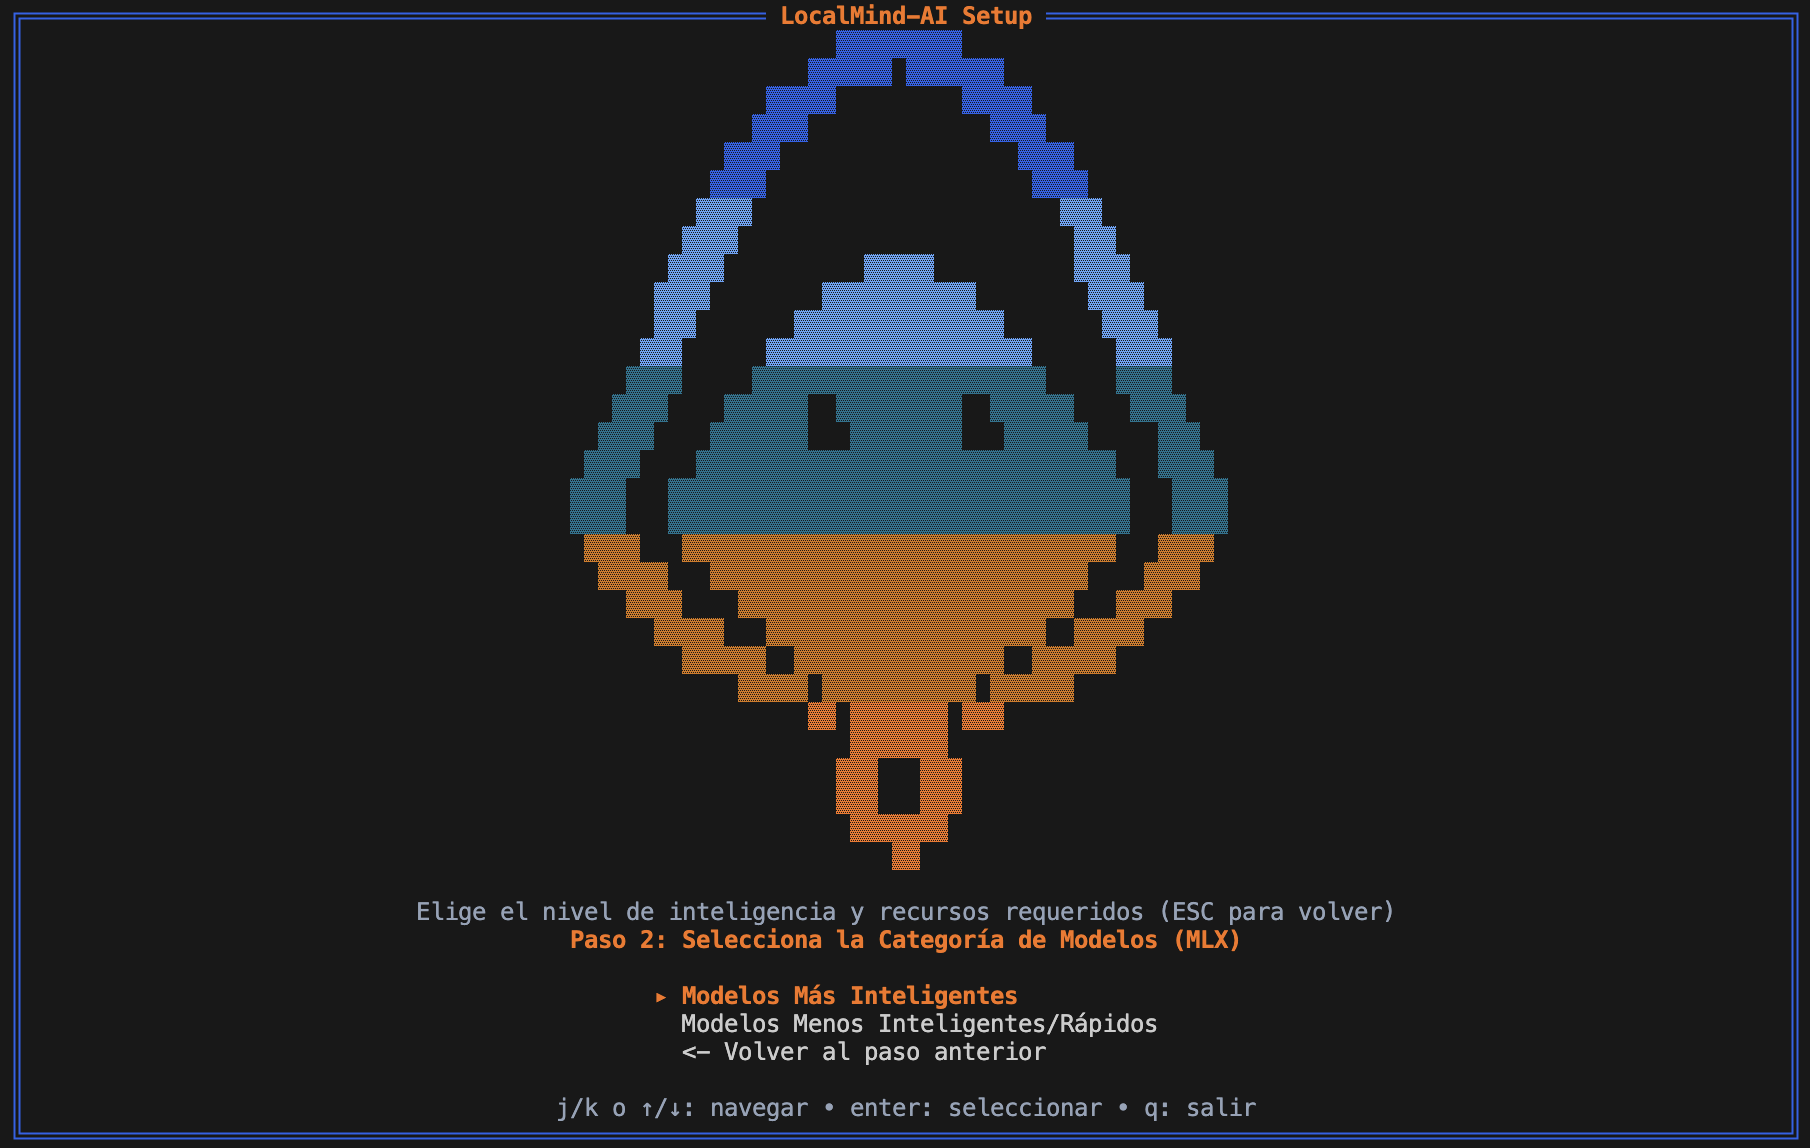
\includegraphics[width=\textwidth]{figs/selector-modelos-ia1.png}
        \caption{Selección por nivel de inteligencia y perfil del modelo.}
        \label{fig:TUITiposModelos}
    \end{subfigure}
    \hfill
    \begin{subfigure}[b]{0.48\textwidth}
        \centering
        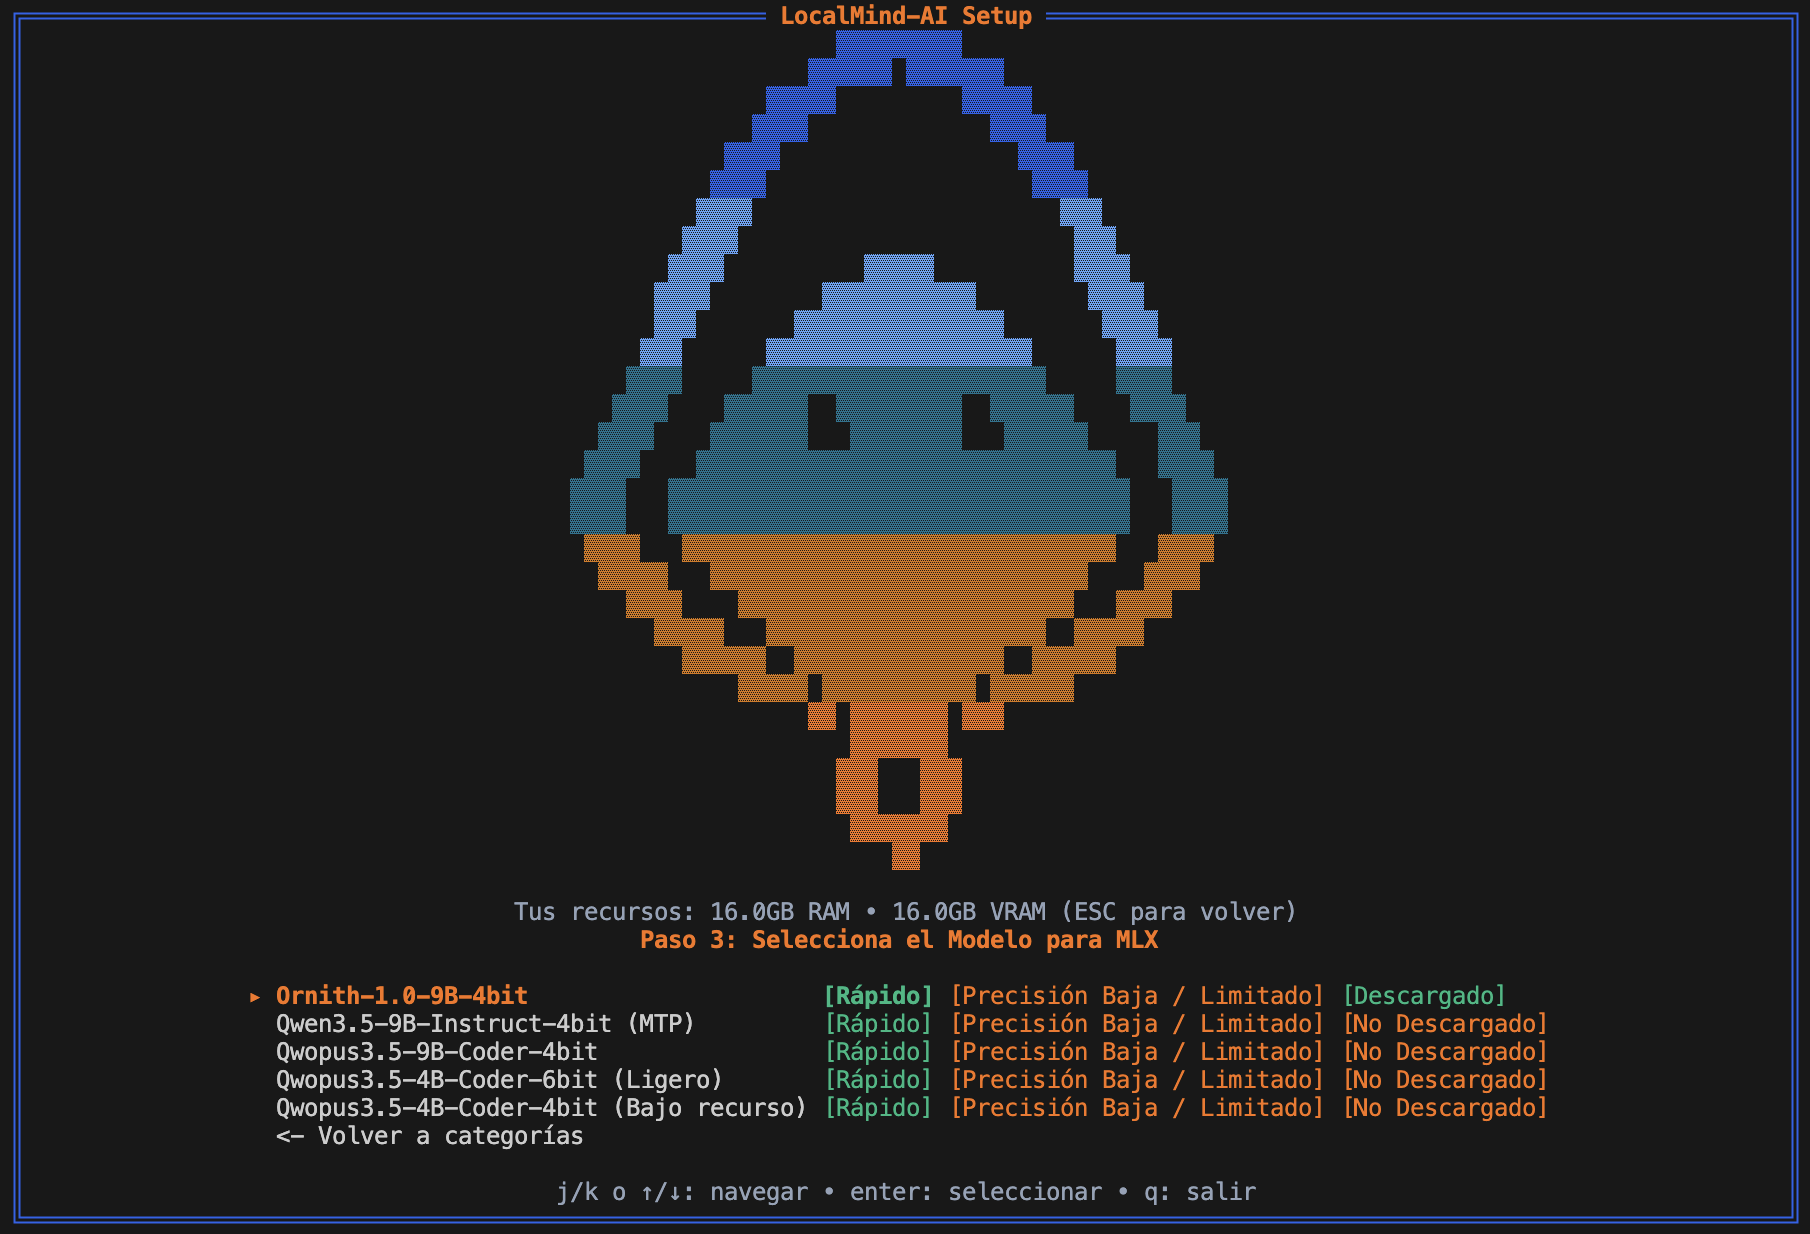
\includegraphics[width=\textwidth]{figs/selector-modelos-ia2.png}
        \caption{Catálogo de modelos con descripción y cuantización comentada.}
        \label{fig:TUIModelosCuantizacion}
    \end{subfigure}
    \caption{Pantallas del selector de modelos e inferencia en la TUI de LocalMind-AI.}
    \label{fig:TUISelectorModelos}
\end{figure}

\subsubsection{Recuperación, memoria y herramientas}\label{subsec:recuperacion-memoria-localmind}

Estos componentes cumplen funciones complementarias en el sistema. Para la base de datos vectorial, \Gls{chromadb} permite guardar documentos, incrustaciones y metadatos en una base de datos integrada, mientras que FAISS es una biblioteca de búsqueda y Qdrant requiere un servidor independiente \cite{chroma2026,faiss2026,qdrant2026}. Se elige \gls{chromadb} para no tener que administrar un servicio de base de datos adicional.

Para generar los \glspl{embeddings}, hacerlo en local garantiza la privacidad al no enviar documentos fuera del equipo. LocalMind utiliza el servicio de \glspl{embeddings} de \gls{ollama}, de modo que el proceso \gls{rag} mantiene esta dependencia incluso si el modelo conversacional se ejecuta con \gls{omlx} \cite{ollamaembeddings2026}.

Para ampliar las funciones del agente, el protocolo \gls{mcp} estandariza el uso de herramientas. Para guardar la conversación, los archivos \gls{jsonl} registran el historial de las sesiones, los ficheros \gls{markdown} guardan la memoria en un formato fácil de leer y el sistema \gls{engram} aporta búsqueda semántica sobre notas anteriores.

\textbf{Decisión.} Se combinan \gls{chromadb}, \glspl{embeddings} locales con \gls{ollama}, herramientas \gls{mcp}, sesiones en \gls{jsonl}, memoria en \gls{markdown} y \gls{engram}, manteniendo clara la función de cada elemento. El flujo de indexación y recuperación documental de LocalMind-AI sigue el esquema conceptual introducido en la Figura~\ref{fig:pipelineRag}, adaptando las fases de fragmentación, incrustación semántica y búsqueda por similitud vectorial a un entorno de ejecución íntegramente local.

En la Figura~\ref{fig:ListadoHerramientasMCP} se expone la pantalla de la TUI de LocalMind-AI correspondiente al listado de herramientas \gls{mcp} registradas y disponibles para el agente.

\begin{figure}[h!tp]
    \centering
    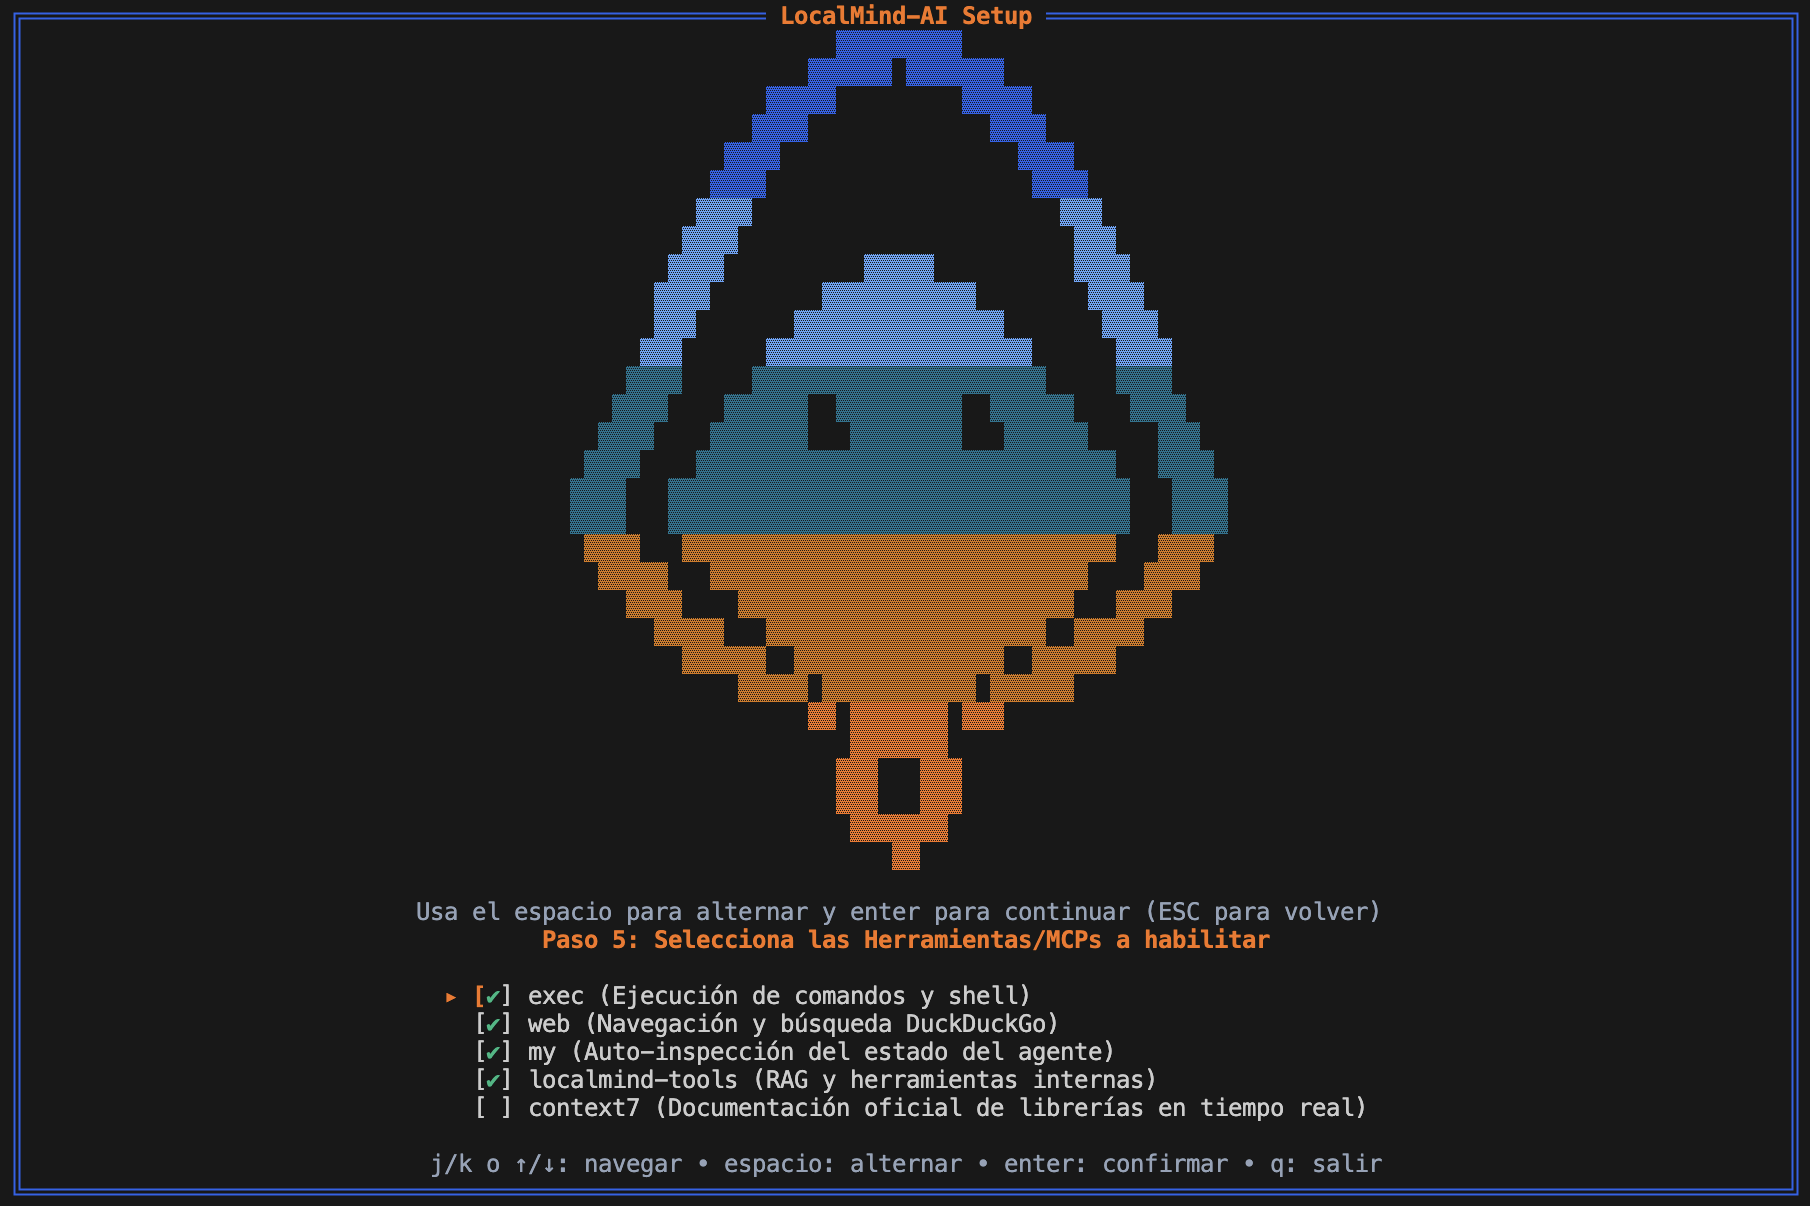
\includegraphics[width=0.82\textwidth]{figs/listado-herramientas-localmind.png}
    \caption{Listado de herramientas MCP integradas y disponibles en la TUI de LocalMind-AI.}
    \label{fig:ListadoHerramientasMCP}
\end{figure}

\subsection{Entorno de desarrollo, gestión de versiones y diseño de diagramas}\label{subsec:entorno-calidad-localmind}

La memoria se redacta en \gls{latex} con Visual Studio Code y se compila localmente con \gls{mactex}. La herramienta Arara automatiza el proceso con pdfLaTeX, Biber y las pasadas necesarias para referencias y glosarios \cite{LaTeXDocumentPreparation,VisualStudioCode,mactex2026,IslandoftexArara2025}, permitiendo trabajar sin depender de un editor web. En la Figura~\ref{fig:visual-mactex-compiler} se observa la interfaz del entorno de desarrollo integrado Visual Studio Code junto con el flujo de compilación local y las herramientas auxiliares empleadas para construir el documento.

Las referencias bibliográficas se gestionan con Zotero, mientras que BibLaTeX y Biber procesan el archivo \texttt{references.bib} durante la compilación \cite{ZoteroYourPersonal,biber2026}. El control de versiones se realiza con Git y GitHub como repositorio remoto \cite{git2026,GitHubcomDocumentacionAyuda}. Asimismo, Visual Studio Code se utiliza para escribir el código en Python, JavaScript, Shell, YAML y los diagramas.

Para la creación de diagramas se utilizan Visual Paradigm, Mermaid y PlantUML \cite{IdealModelingDiagramming,Mermaid,plantuml2026}, elaborando el diagrama de Gantt del proyecto únicamente con PlantUML.

\textbf{Decisión.} El entorno de desarrollo está formado por Visual Studio Code, LaTeX, MacTeX, Arara, Zotero, Biber, Git, GitHub, Visual Paradigm, Mermaid y PlantUML. Cada herramienta se selecciona por su utilidad práctica dentro del proyecto.

\begin{figure}[h!tp]
    \centering
    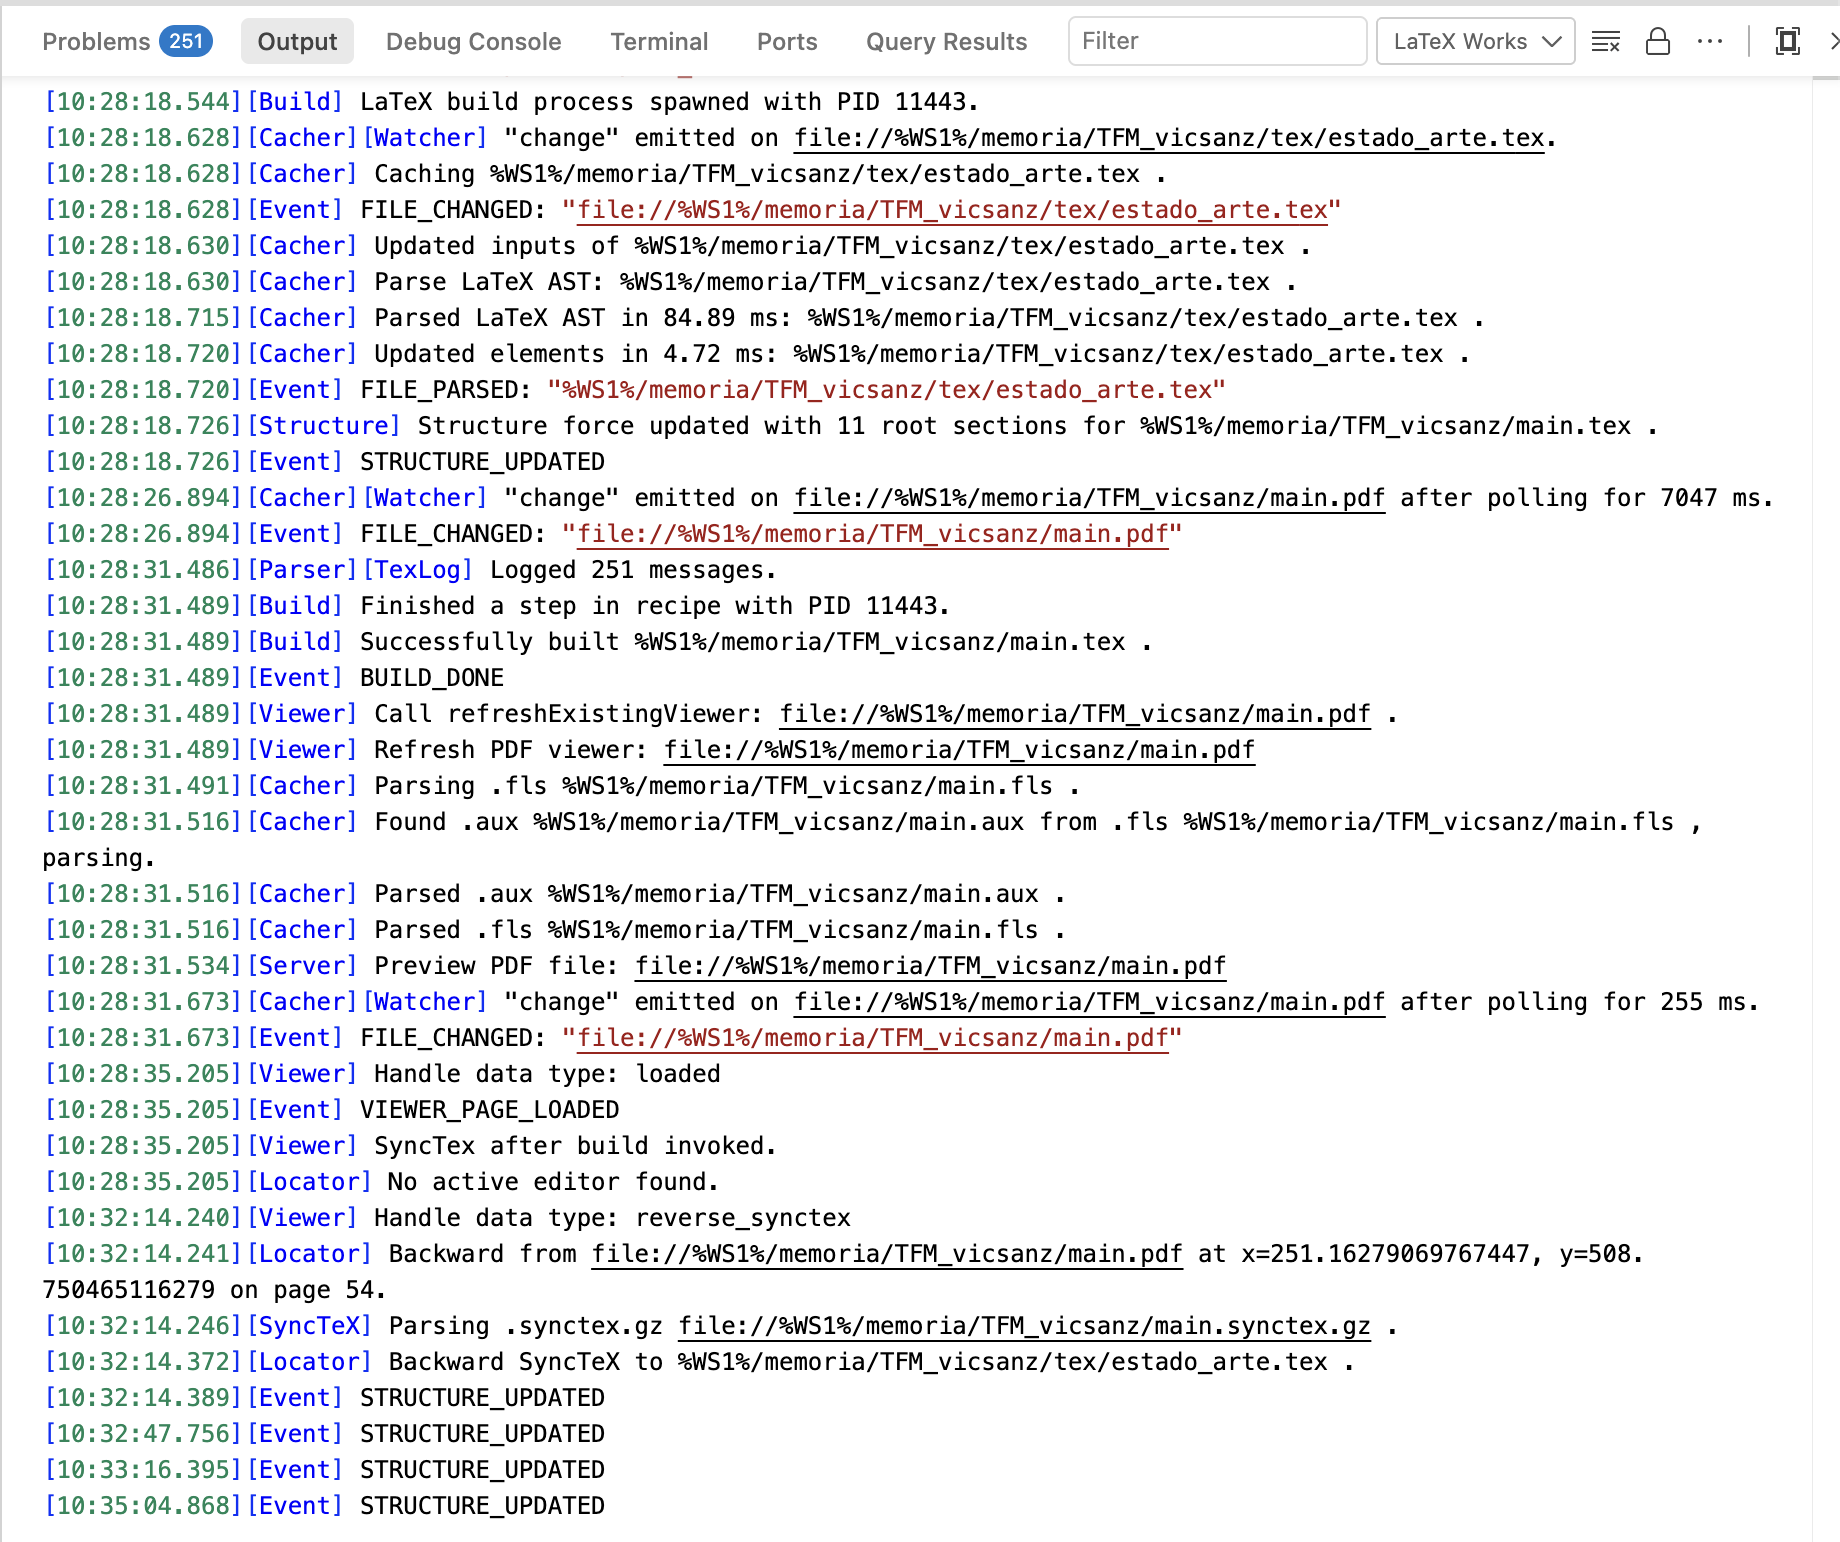
\includegraphics[width=0.80\textwidth]{figs/visual_mactex_compiler.png}
    \caption{Entorno de desarrollo empleado para compilar la memoria.}
    \label{fig:visual-mactex-compiler}
\end{figure}

\subsection{Conclusiones}\label{subsec:conclusiones-evaluacion-localmind}

La evaluación de tecnologías define una arquitectura modular y práctica. Docker Compose separa el agente y el cliente web en dos servicios: \gls{nanobot} concentra la comunicación y las herramientas, mientras que \gls{nginx} sirve los activos estáticos exportados por \gls{expo}. El navegador se comunica directamente con el agente mediante \gls{websocket} y \gls{rest}, y los modelos se procesan en el sistema anfitrión para aprovechar su aceleración. La memoria y el almacenamiento, por su parte, se dividen en componentes específicos. En la Tabla~\ref{tab:tecnologias-localmind} se resumen las decisiones tecnológicas adoptadas en el proyecto.

\begin{sidewaystable}[h!tp]
    \centering
    \scriptsize
    \setlength{\tabcolsep}{5pt}
    \renewcommand{\arraystretch}{1.12}
    \begin{tabularx}{\textwidth}{|>{\raggedright\arraybackslash}p{3.1cm}|>{\raggedright\arraybackslash}p{5.1cm}|>{\raggedright\arraybackslash}X|}
        \hline
        \textbf{Tipo}                    & \textbf{Necesidad}        & \textbf{Componente}                                                                                             \\
        \hline
        \multirow{2}{=}{Hardware}        & Portátiles de validación  & MSI Pulse GL66 12UEK-085ES y MacBook Air M4                                                                     \\
        \cline{2-3}
                                         & Referencia descartada     & HP OMEN 15-ce033ns, insuficiente para la validación prevista                                                    \\
        \hline
        \multirow{4}{=}{Infraestructura} & Sistemas anfitriones      & \Gls{windows}, \gls{macos} y compatibilidad \gls{linux}                                                         \\
        \cline{2-3}
                                         & Contenedores              & \Gls{docker}                                                                                                    \\
        \cline{2-3}
                                         & Despliegue reproducible   & \Gls{dockercompose} con servicios \texttt{nanobot} y \texttt{frontend}; \gls{mcp}/\gls{engram} como subprocesos \\
        \cline{2-3}
                                         & Aceleración               & \Gls{ollama} u \gls{omlx}/\gls{mlx} ejecutados nativamente en el host                                           \\
        \hline
        \multirow{12}{=}{Software}       & Lenguajes del producto    & \Gls{python}, \gls{javascript}, Shell/\gls{bash} y \gls{yaml}                                                   \\
        \cline{2-3}
                                         & Cliente web               & \Gls{reactnative} Web con \gls{expo}, exportado y servido por \gls{nginx}                                       \\
        \cline{2-3}
                                         & Núcleo del agente         & \Gls{nanobot}                                                                                                   \\
        \cline{2-3}
                                         & API y comunicación        & \gls{aiohttp}, \gls{websocket} y \gls{rest}                                                                     \\
        \cline{2-3}
                                         & Instalador/configurador   & \Gls{tui} \gls{python} con \gls{ansi}, inspirada en Gentle-AI                                                   \\
        \cline{2-3}
                                         & Inferencia local          & \Gls{ollama} y \gls{omlx}/\gls{mlx}                                                                             \\
        \cline{2-3}
                                         & Modelos                   & Ornith 1.0 9B y Qwen 3.5 9B, cuantizaciones de 4/6 bits                                                         \\
        \cline{2-3}
                                         & Recuperación documental   & \Gls{chromadb} y \glspl{embeddings} locales mediante \gls{ollama}                                               \\
        \cline{2-3}
                                         & Herramientas y memoria    & \Gls{mcp}, \gls{engram}, \gls{jsonl} y \gls{markdown}                                                           \\
        \cline{2-3}
                                         & Memoria y referencias     & LaTeX, MacTeX, Arara, Zotero y Biber                                                                            \\
        \cline{2-3}
                                         & Versionado y desarrollo   & Git, GitHub y Visual Studio Code                                                                                \\
        \cline{2-3}
                                         & Diagramas y planificación & Visual Paradigm, Mermaid y PlantUML, Gantt con PlantUML                                                         \\
        \hline
    \end{tabularx}
    \caption{Tecnologías seleccionadas para el desarrollo y la validación de LocalMind-AI.}
    \label{tab:tecnologias-localmind}
\end{sidewaystable}


\chapter{Requisitos, especificaciones, coste, riesgos y viabilidad}\label{ch:requisitos}
% Contenidos del capítulo
% Las secciones presentadas son orientativas y no representan
% necesariamente la organización que debe tener este capítulo.

\section{Requisitos}

En este capítulo se establecen los requisitos y las especificaciones de LocalMind-AI, un asistente de \gls{ia} orientado a la ejecución local. La definición parte del análisis del prototipo y de su arquitectura actual, pero se formula como un contrato verificable, por el que los requisitos expresan el comportamiento y las cualidades que deberá demostrar el sistema, no resultados que se consideren ya acreditados. Los objetivos cuantitativos se contrastarán posteriormente sobre los equipos de validación previstos.

La propuesta adopta un enfoque \gls{localfirst}, por el que la inferencia, los documentos y la memoria permanecen en el equipo de la persona usuaria de forma predeterminada \cite{kleppmann2019local}. Las integraciones que requieren acceder a servicios externos se consideran opcionales y solo podrán habilitarse tras una acción consciente y explícita. A partir de este principio se distinguen los requisitos funcionales, que describen las capacidades observables, y los requisitos no funcionales, que fijan restricciones y criterios de calidad.

\subsection{Requisitos funcionales}

Los requisitos funcionales definen las operaciones que LocalMind-AI deberá poner a disposición del usuario para las tareas de instalación, configuración y uso.

\begin{itemize}
    \item[\textbf{RF1.}] \textbf{Interacción conversacional y transparencia CoT.} El sistema deberá ofrecer un chat conversacional que muestre en tiempo real las respuestas incrementales del \gls{llm} y los pasos intermedios de razonamiento (\gls{cot}), indicando claramente cuándo el agente realiza reflexiones internas, consulta la memoria o invoca herramientas.
    \item[\textbf{RF2.}] \textbf{Gestión de conversaciones y tareas.} El sistema deberá permitir iniciar nuevas conversaciones, pausar o cancelar generaciones en curso, mantener el historial de mensajes por sesión, consultar y editar tareas asociadas y eliminar sesiones de forma segura.
    \item[\textbf{RF3.}] \textbf{Gestión y conmutación de modelos.} El sistema deberá permitir seleccionar y alternar dinámicamente el modelo de lenguaje en ejecución (\gls{ollama} o \gls{omlx}), validar la conectividad con el servidor de inferencia y adaptar la interfaz según el perfil de modelo activo.
    \item[\textbf{RF4.}] \textbf{Ingesta y procesamiento de documentos.} El sistema deberá permitir la carga de archivos en formatos \gls{pdf} y \gls{markdown}, su división en fragmentos semánticamente coherentes mediante \textit{recursive character text splitter} y su indexación vectorial en \gls{chromadb}.
    \item[\textbf{RF5.}] \textbf{Recuperación semántica (\gls{rag}).} El sistema deberá transformar las consultas del usuario en vectores de \gls{embeddings}, recuperar los $k$ fragmentos de código o documentación más relevantes de \gls{chromadb} e inyectarlos en el contexto del \gls{llm} para fundamentar la respuesta.
    \item[\textbf{RF6.}] \textbf{Configuración de parámetros \gls{rag}.} La interfaz deberá permitir ajustar el número de fragmentos a recuperar ($k$), el umbral de similitud semántica, el tamaño de fragmento (\textit{chunk size}) y el solapamiento (\textit{overlap}).
    \item[\textbf{RF7.}] \textbf{Persistencia de memoria semántica.} El sistema deberá integrar \gls{engram} para almacenar observaciones, aprendizajes y notas de la sesión, permitiendo la búsqueda por similitud sobre experiencias previas y su inyección transparente en el \gls{prompt} del agente.
    \item[\textbf{RF8.}] \textbf{Persistencia de sesiones y memoria.} El sistema deberá almacenar y recuperar el historial de las conversaciones mediante ficheros \gls{jsonl} y \gls{markdown}, y deberá permitir habilitar \gls{engram} como memoria persistente adicional. También deberá ofrecer mecanismos selectivos para eliminar estos datos.
    \item[\textbf{RF9.}] \textbf{Uso de herramientas.} El \gls{agenteia} deberá descubrir, habilitar e invocar herramientas proporcionadas mediante \gls{mcp}. El alcance funcional incluirá la generación de documentos \gls{pdf} y el almacenamiento de los artefactos resultantes en el equipo local. Las operaciones protegidas, como la ejecución de órdenes o la modificación de archivos, deberán requerir confirmación previa de la persona usuaria.
    \item[\textbf{RF10.}] \textbf{Seguimiento y recuperación.} La interfaz deberá comunicar los errores de conexión o ejecución, reintentar la conexión sin perder la sesión y mostrar un resumen comprensible de las etapas realizadas y de las herramientas utilizadas, sin exponer el contenido interno completo de la \gls{cot}.
\end{itemize}

\subsection{Requisitos no funcionales}

Los siguientes requisitos establecen criterios de calidad y umbrales de aceptación. Los valores temporales, de usabilidad y de consumo constituyen objetivos pendientes de validación en el apartado de pruebas de esta memoria.

\begin{itemize}
    \item[\textbf{RNF1.}] \textbf{Privacidad y funcionamiento local.} Los mensajes, documentos, índices, memorias e inferencias deberán procesarse localmente de forma predeterminada. Cualquier herramienta que transmita información fuera del equipo deberá permanecer deshabilitada hasta que la persona usuaria la active o autorice explícitamente.
    \item[\textbf{RNF2.}] \textbf{Latencia.} En las pruebas con el modelo de referencia, el percentil 90 del tiempo transcurrido hasta recibir el primer fragmento de una respuesta incremental deberá ser inferior o igual a 10 segundos. El cumplimiento se medirá por separado en el MSI Pulse GL66 y en el MacBook Air M4.
    \item[\textbf{RNF3.}] \textbf{Uso de recursos.} El servicio de \gls{nanobot} ejecutado en su contenedor tendrá un límite de 4~GiB de memoria. El consumo del contenedor \texttt{frontend} se evaluará de manera independiente y su imagen de ejecución no deberá conservar las dependencias utilizadas para construir el cliente. La selección del modelo deberá tener en cuenta la memoria principal y la memoria de vídeo disponibles, mientras que el consumo del motor de inferencia nativo se medirá por separado.
    \item[\textbf{RNF4.}] \textbf{Operación sin conexión.} Una vez instaladas las dependencias y descargados los modelos, el chat, la recuperación documental, la memoria y las herramientas locales deberán funcionar sin conexión a Internet. Las integraciones externas deberán indicar claramente su estado no disponible, sin impedir el uso de las funciones locales.
    \item[\textbf{RNF5.}] \textbf{Seguridad de red, privilegios y secretos.} Los servicios deberán enlazarse de forma predeterminada a la interfaz de red de bucle local. El contenedor de \gls{nanobot} deberá ejecutarse con un usuario sin privilegios, sin extender esta garantía a componentes que no se hayan validado. Una eventual exposición remota requerirá autenticación y cifrado mediante \gls{tls}; las credenciales no deberán almacenarse en el código fuente ni aparecer en respuestas o registros. Estas medidas se revisarán tomando como referencia las recomendaciones de \gls{owasp} \cite{OWASPTopTen}.
    \item[\textbf{RNF6.}] \textbf{Protección de acciones.} La ejecución de órdenes y la escritura, edición o eliminación de archivos deberán solicitar confirmación previa y limitarse al espacio de trabajo o a la política de aislamiento configurados.
    \item[\textbf{RNF7.}] \textbf{Fiabilidad de la comunicación.} Ante una interrupción recuperable, el cliente deberá restablecer la conexión en un máximo de 5 segundos, conservar la sesión activa y evitar la duplicación de solicitudes o resultados.
    \item[\textbf{RNF8.}] \textbf{Usabilidad.} La evaluación deberá alcanzar una puntuación \gls{sus} igual o superior a 68 y una tasa de éxito igual o superior al 80\,\% en las tareas de iniciar una conversación, cambiar el modelo y localizar un artefacto generado.
    \item[\textbf{RNF9.}] \textbf{Compatibilidad.} El cliente deberá funcionar en navegadores web modernos y los lanzadores deberán admitir \gls{macos}, \gls{linux} y \gls{windows}. \gls{omlx} se destinará a equipos Apple Silicon y \gls{ollama} constituirá la alternativa general.
    \item[\textbf{RNF10.}] \textbf{Reproducibilidad.} La instalación sobre un entorno limpio deberá poder completarse mediante el lanzador y la \gls{tui}, sin exigir la edición manual de los archivos de configuración generados. El cliente web deberá poder construirse y arrancarse mediante \gls{docker}, sin requerir \gls{nodejs}, \gls{pnpm} ni un directorio \texttt{node\_modules} como dependencias finales instaladas en el anfitrión.
    \item[\textbf{RNF11.}] \textbf{Mantenibilidad y extensibilidad.} Los módulos deberán estar documentados y seguir \gls{pep8} y los principios \gls{solid} \cite{PEP8Style,SOLIDPrinciplesCinco2025}. La incorporación de un nuevo proveedor de inferencia o servidor \gls{mcp} no deberá requerir modificaciones en el núcleo de la conversación.
    \item[\textbf{RNF12.}] \textbf{Persistencia.} El espacio de trabajo, las sesiones, la colección de \gls{chromadb}, la memoria de \gls{engram} y los artefactos generados por \gls{nanobot} deberán conservarse tras reiniciar o recrear los contenedores. Las operaciones de limpieza selectiva deberán afectar únicamente al almacén elegido.
    \item[\textbf{RNF13.}] \textbf{Observabilidad.} Los diagnósticos, indicadores de estado, comprobaciones de salud y registros deberán reflejar por separado la disponibilidad del cliente servido por \gls{nginx}, del agente, del motor de inferencia, de los servidores \gls{mcp} y de los almacenes persistentes, sin revelar datos sensibles.
    \item[\textbf{RNF14.}] \textbf{Trazabilidad y calidad.} Cada requisito funcional y no funcional deberá asociarse en la fase de validación con una prueba o evidencia reproducible. La clasificación de las características de calidad seguirá el modelo ISO/IEC~25010 \cite{ISOIEC25010}.
\end{itemize}

\section{Especificaciones}\label{sec:especificaciones-sistema}

A partir de los requisitos anteriores, LocalMind-AI se especifica como un sistema personal de asistencia local cuyo actor principal es una persona con conocimientos técnicos que instala, configura y utiliza el mismo entorno. No se establecen roles independientes de administración ni un modelo multiusuario. La solución se organiza en cuatro subsistemas, que corresponden a interacción, comunicación, aplicación y servicios locales. La Figura~\ref{fig:localmind-overview} resume su relación y diferencia mediante trazo discontinuo las integraciones externas, que son opcionales y requieren consentimiento.

\begin{figure}[htbp]
    \centering
    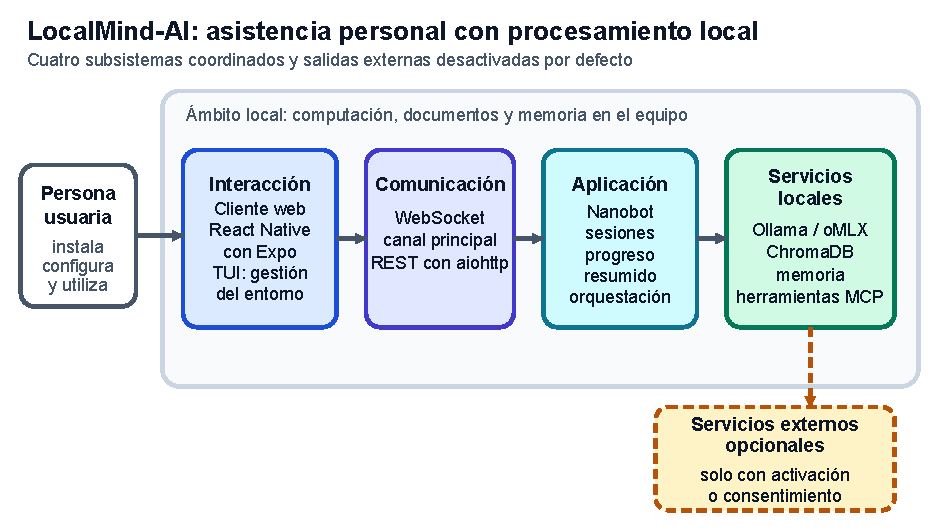
\includegraphics[width=0.95\textwidth]{figs/localmind-overview.pdf}
    \caption{Mapa conceptual de LocalMind-AI.}
    \label{fig:localmind-overview}
\end{figure}

El entorno de ejecución se distribuye entre el navegador, el equipo anfitrión y dos servicios gestionados mediante \gls{dockercompose}. Como representa la Figura~\ref{fig:localmind-runtime}, el servicio \texttt{frontend} contiene los activos estáticos exportados por \gls{expo} y los sirve mediante \gls{nginx} en el puerto 8081, mientras que el servicio \texttt{nanobot} aloja el agente, la pasarela \gls{websocket}, la \gls{api} \gls{rest} y las herramientas integradas. La imagen del agente se construye en varias etapas y su proceso se ejecuta con el usuario no privilegiado \texttt{nanobot} \cite{docker2026multistage}. Los servidores \gls{mcp}, incluido \gls{engram} cuando está habilitado, se inician dentro de ese contenedor como subprocesos configurados y no como servicios adicionales de Compose. \Gls{ollama} o \gls{omlx}, servidor basado en MLX, permanecen en el anfitrión para aprovechar la aceleración disponible y son accesibles desde el agente mediante \texttt{host.docker.internal} \cite{docker2024compose}.

\Gls{nginx} se limita a entregar la aplicación web y no actúa como proxy inverso de los canales del agente \cite{nginx2026}. Después de descargar los activos desde \texttt{http://localhost:8081}, el navegador establece directamente con \gls{nanobot} la conexión \gls{websocket} del puerto 8765 o las peticiones \gls{rest} del puerto 8900. Como parte del diseño previsto, los volúmenes deberán separar el espacio de trabajo, las sesiones, los resultados, la colección vectorial y la memoria, además de conservar los datos exigidos por el RNF12 tras reinicios o recreaciones. Este comportamiento y las comprobaciones de salud definidas por el RNF13 permanecen pendientes de validación.

\begin{figure}[htbp]
    \centering
    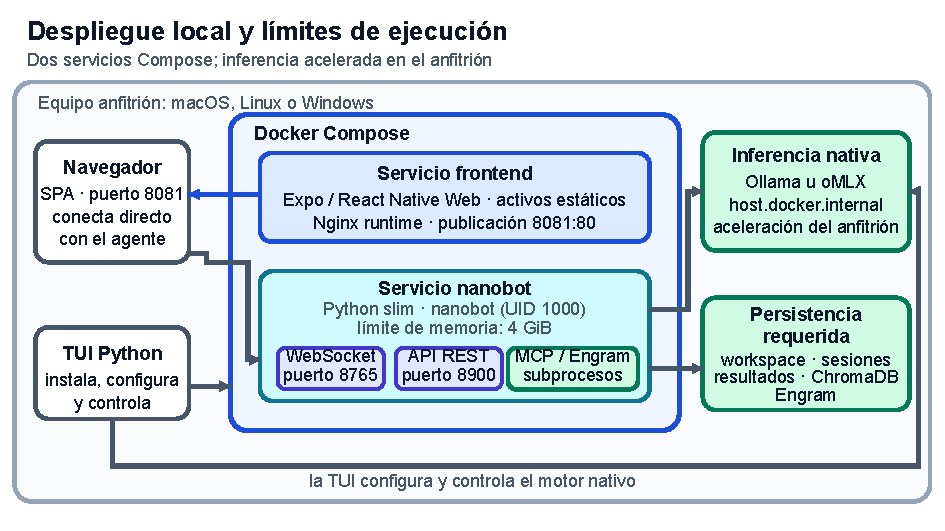
\includegraphics[width=0.95\textwidth]{figs/localmind-runtime.pdf}
    \caption{Entorno de ejecución local de LocalMind-AI.}
    \label{fig:localmind-runtime}
\end{figure}

La capa de interacción ofrece dos puntos de entrada complementarios, pero con responsabilidades distintas. El cliente desarrollado con \gls{reactnative} y \gls{expo}, exportado como aplicación web estática y servido por \gls{nginx}, proporciona la conversación en el navegador, la selección del modelo y la consulta de resultados \cite{meta2024reactnative,expo2024,nginx2026}. Una vez cargado, este cliente se conecta directamente con el servidor \gls{websocket} de \gls{nanobot} como canal principal para recibir eventos y fragmentos de respuesta, y dispone de una \gls{api} \gls{rest}, implementada con \gls{aiohttp} y compatible con el formato de conversación de OpenAI, como alternativa \cite{aiohttp2026,rfc6455}. Por separado, la \gls{tui}, implementada en \gls{python}, concentra la instalación, la configuración, el diagnóstico y el control operativo de \gls{dockercompose} y del motor nativo, por lo que no actúa como un cliente conversacional de esos dos canales. Esta separación se sintetiza en la Figura~\ref{fig:localmind-interaction}.

\begin{figure}[htbp]
    \centering
    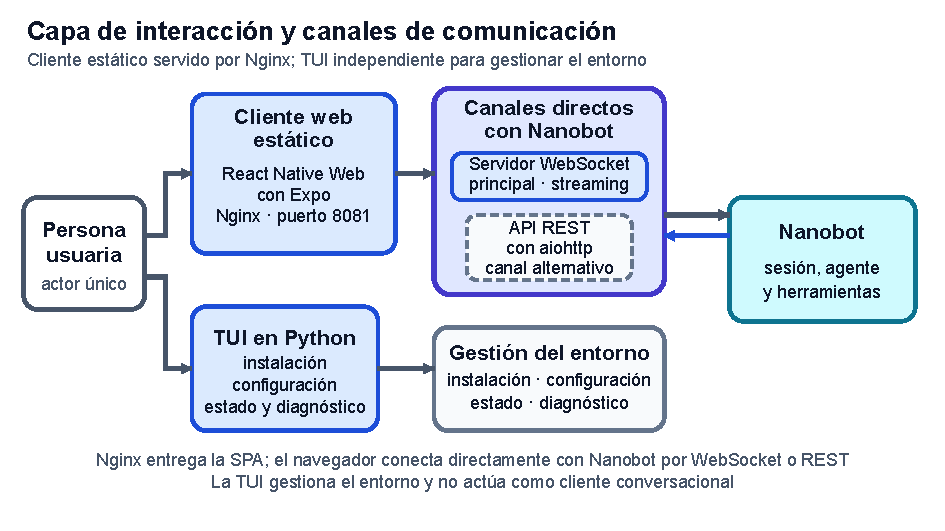
\includegraphics[width=0.95\textwidth]{figs/localmind-interaction.pdf}
    \caption{Mapa conceptual de la capa de interacción.}
    \label{fig:localmind-interaction}
\end{figure}

La capa de aplicación está constituida por \gls{nanobot}, que mantiene el contexto de la sesión, coordina las llamadas al modelo y selecciona las herramientas necesarias \cite{nanobot2026}. Según el flujo conceptual de la Figura~\ref{fig:localmind-agent}, cada petición se vincula primero con una sesión y, a continuación, el agente decide si puede responder mediante inferencia directa, si necesita recuperar documentación o si debe invocar una herramienta. Como comportamiento requerido, la interfaz deberá recibir estados resumidos y los nombres de las herramientas empleadas, pero no el razonamiento interno completo del modelo. Asimismo, los errores deberán convertirse en estados comprensibles y las acciones protegidas deberán introducir un punto de confirmación antes de continuar. El cumplimiento de este seguimiento visible y de la recuperación ante fallos queda pendiente de validación.

\begin{figure}[htbp]
    \centering
    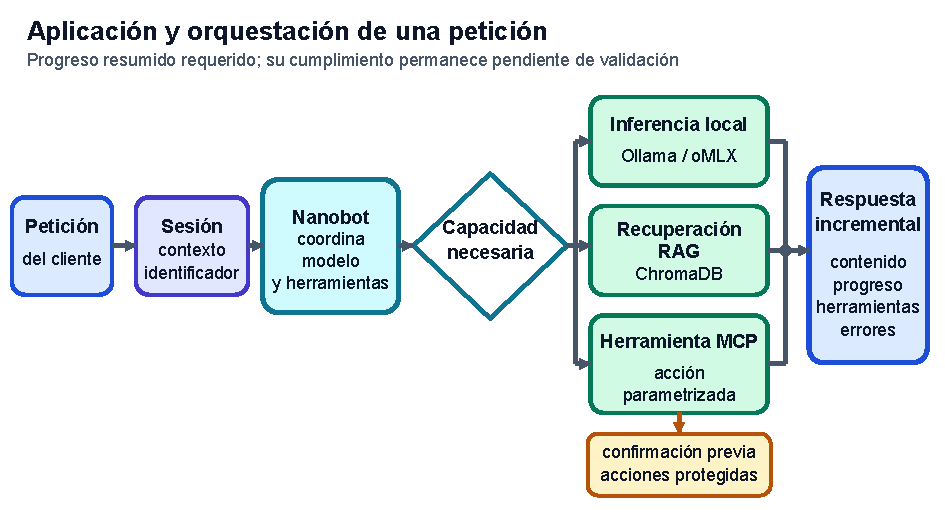
\includegraphics[width=0.95\textwidth]{figs/localmind-agent.pdf}
    \caption{Mapa conceptual de la capa de aplicación y orquestación.}
    \label{fig:localmind-agent}
\end{figure}

La capa de servicios, representada en la Figura~\ref{fig:localmind-services}, mantiene responsabilidades diferenciadas. \Gls{ollama} y \gls{omlx}, este último como servidor basado en \gls{mlx}, proporcionan inferencia local, \gls{chromadb} conserva los vectores empleados por \gls{rag}, los ficheros \gls{jsonl} y \gls{markdown} registran las sesiones, y \gls{engram} aporta, cuando se activa, una memoria semántica de mayor duración. Por su parte, \gls{mcp} normaliza el acceso del agente a herramientas locales o externas e incluye capacidades reales para generar documentos \gls{pdf} y guardar los artefactos correspondientes en el almacenamiento local \cite{ollama2024,omlx2026,chroma2026,anthropic2024mcp}. Estas piezas no son alternativas equivalentes, ya que cada una resuelve una responsabilidad distinta y puede evolucionar sin alterar el canal de interacción.

\begin{figure}[htbp]
    \centering
    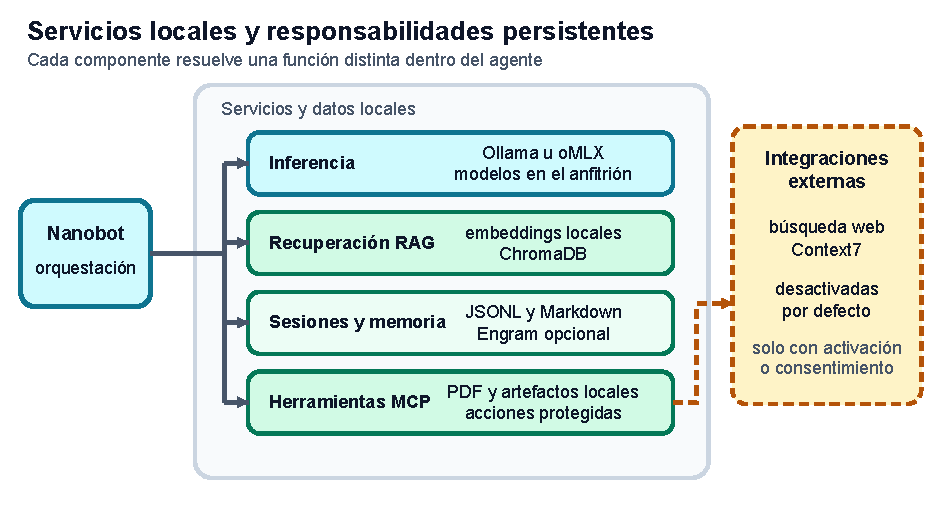
\includegraphics[width=0.95\textwidth]{figs/localmind-services.pdf}
    \caption{Mapa conceptual de los servicios locales.}
    \label{fig:localmind-services}
\end{figure}

La especificación excluye del alcance actual las cuentas de usuario, la administración remota y la infraestructura como servicio.

\FloatBarrier
\section{Costes}
% Costes temporales y económicos
En este apartado se presenta la planificación temporal del proyecto y se estima el coste económico asociado a su desarrollo. Para ello, se describe el ciclo de vida adoptado, se descompone el trabajo en actividades verificables y se valoran tanto la dedicación del autor como los medios materiales utilizados.

La elección de una metodología adecuada resulta necesaria para organizar el trabajo y controlar sus posibles desviaciones. Las \glspl{metagil} \cite{ilievaAnalysesAgileMethodology2004}, entre las que se encuentran \gls{scrum} y \gls{kanban}, favorecen ciclos breves, una adaptación continua y la interacción frecuente con las partes interesadas. Frente a ellas, los enfoques iterativos e incrementales estructuran el desarrollo en sucesivas revisiones de análisis, diseño, implementación y prueba, de forma que cada incremento se apoya en resultados previamente consolidados.

En LocalMind-AI se ha adoptado una \gls{iterativa} \cite{larmanIterativeIncrementalDevelopments2003}. Esta elección responde al carácter individual del proyecto y a la necesidad de validar de manera progresiva componentes con dependencias distintas, como el cliente web, el agente, la recuperación documental y los motores de inferencia. El enfoque conserva una planificación estructurada, pero permite revisar decisiones técnicas cuando una prueba de integración o una ejecución en otra plataforma revela una limitación no prevista.

El ciclo de vida se divide en seis fases principales. La fase de \textbf{documentación} comprende la revisión del estado del arte, la elaboración de prototipos y la redacción continuada de la memoria. La fase de \textbf{análisis} concreta los requisitos y las especificaciones. Durante el \textbf{diseño} se definen la arquitectura \gls{localfirst}, la interacción mediante el cliente web y la \gls{tui}, la comunicación, el agente, la recuperación documental y la inferencia local. La \textbf{implementación} materializa esos componentes e integra los dos servicios de \gls{dockercompose} con los motores que permanecen en el anfitrión. El \textbf{despliegue} prepara un entorno reproducible y comprueba la instalación en los dos equipos de validación. Por último, las \textbf{pruebas} reúnen la verificación funcional, de integración, rendimiento, recursos, usabilidad y seguridad.

La estimación de las actividades se ha realizado mediante la técnica \gls{pert} \cite{mazlumCPMPERTProject2015}. Esta técnica combina una duración optimista (\(O\)), una pesimista (\(P\)) y una duración más probable (\(M\)). La Ecuación~\ref{eq:tecnicaPERT} obtiene la duración esperada \(E\) mediante una media ponderada que concede mayor peso al escenario más probable.

% Ecuación técnica PERT.
\begin{equation}
    E = \frac{O + P + 4M}{6}
    \label{eq:tecnicaPERT}
\end{equation}

El desarrollo del \gls{tfm} se compagina con una jornada laboral ordinaria de ocho horas diarias en una empresa. Esas cuarenta horas semanales no forman parte del esfuerzo del proyecto y limitan la disponibilidad a los periodos indicados en la Tabla~\ref{tab:horarioTFM}. Se mantiene una dedicación de dos horas los jueves y viernes y de cuatro horas los sábados y domingos, lo que proporciona doce horas semanales.

% Tabla de horario de dedicación al TFM.
\begin{table}[h!tp]
    \centering
    \begin{adjustbox}{max width=\textwidth}
        \begin{tabular}{|c|c|c|c|c|c|c|c|}
            \hline
            Lunes & Martes & Miércoles & Jueves & Viernes & Sábado & Domingo & Total \\ \hline
            0 h   & 0 h    & 0 h       & 2 h    & 2 h     & 4 h    & 4 h     & 12 h  \\ \hline
        \end{tabular}
    \end{adjustbox}
    \caption{Horario semanal de dedicación al \gls{tfm}.}
    \label{tab:horarioTFM}
\end{table}

La Tabla~\ref{tab:estimacionTareas} recoge las veinticinco actividades previstas. La última columna expresa la duración esperada en semanas de doce horas; el total se calcula a partir de las horas sin redondear, por lo que no depende de la suma de los valores decimales mostrados en cada fila.

\sisetup{
    output-decimal-marker = {,},
    group-separator = {.}
}

\begin{table}[p]
    \centering
    \scriptsize
    \setlength{\tabcolsep}{2.5pt}
    \renewcommand{\arraystretch}{1.12}
    \begin{tabularx}{\textwidth}{
            |>{\raggedright\arraybackslash}p{2.2cm}
            |>{\raggedright\arraybackslash}X
            |S[table-format=2.0]
            |S[table-format=2.0]
            |S[table-format=2.0]
            |S[table-format=3.0]
            |S[table-format=2.2]|
        }
        \hline
        \textbf{Fase}                        & \textbf{Actividad}                                  & {\textbf{T. opt. (h)}} & {\textbf{T. pes. (h)}} & {\textbf{T. más probable (h)}} & {\textbf{Estim. (h)}}               & {\textbf{Semanas}} \\
        \hline
        \multirow{2}{=}{\centering Documentación}
                                             & Estado del arte y prototipos                        & 12                     & 24                     & 18                             & 18                                  & 1.50               \\
                                             & Redacción y revisión de la memoria                  & 18                     & 36                     & 27                             & 27                                  & 2.25               \\
        \hline
        \multirow{2}{=}{\centering Análisis}
                                             & Definición de requisitos                            & 8                      & 16                     & 12                             & 12                                  & 1.00               \\
                                             & Especificación del sistema                          & 10                     & 18                     & 14                             & 14                                  & 1.17               \\
        \hline
        \multirow{6}{=}{\centering Diseño}
                                             & Arquitectura \gls{localfirst} y despliegue          & 10                     & 22                     & 16                             & 16                                  & 1.33               \\
                                             & Interacción web y \gls{tui}                         & 6                      & 14                     & 10                             & 10                                  & 0.83               \\
                                             & Comunicación \gls{websocket}/\gls{rest}             & 6                      & 14                     & 10                             & 10                                  & 0.83               \\
                                             & Agente, \gls{mcp} y memoria                         & 8                      & 16                     & 12                             & 12                                  & 1.00               \\
                                             & \gls{rag}, \gls{chromadb} y \glspl{embeddings}      & 6                      & 14                     & 10                             & 10                                  & 0.83               \\
                                             & Inferencia local y multiplataforma                  & 10                     & 18                     & 14                             & 14                                  & 1.17               \\
        \hline
        \multirow{9}{=}{\centering Implementación}
                                             & \gls{tui} y lanzadores                              & 14                     & 30                     & 22                             & 22                                  & 1.83               \\
                                             & Cliente \gls{expo}/\gls{reactnative} Web            & 16                     & 36                     & 26                             & 26                                  & 2.17               \\
                                             & Exportación estática y \gls{nginx}                  & 8                      & 20                     & 14                             & 14                                  & 1.17               \\
                                             & Pasarela \gls{aiohttp} \gls{websocket}/\gls{rest}   & 16                     & 32                     & 24                             & 24                                  & 2.00               \\
                                             & \gls{rag}, \gls{chromadb} y \glspl{embeddings}      & 12                     & 28                     & 20                             & 20                                  & 1.67               \\
                                             & Sesiones, \gls{jsonl}/\gls{markdown} y \gls{engram} & 10                     & 22                     & 16                             & 16                                  & 1.33               \\
                                             & Herramientas \gls{mcp} y confirmaciones             & 10                     & 22                     & 16                             & 16                                  & 1.33               \\
                                             & Proveedores \gls{ollama}/\gls{omlx}                 & 8                      & 16                     & 12                             & 12                                  & 1.00               \\
                                             & Dockerfiles, Compose e integración                  & 6                      & 14                     & 10                             & 10                                  & 0.83               \\
        \hline
        \multirow{3}{=}{\centering Despliegue}
                                             & Entorno reproducible                                & 6                      & 14                     & 10                             & 10                                  & 0.83               \\
                                             & Validación MSI/\gls{windows}                        & 6                      & 14                     & 10                             & 10                                  & 0.83               \\
                                             & Validación MacBook/\gls{macos}                      & 6                      & 14                     & 10                             & 10                                  & 0.83               \\
        \hline
        \multirow{3}{=}{\centering Pruebas}
                                             & Pruebas funcionales e integración                   & 6                      & 14                     & 10                             & 10                                  & 0.83               \\
                                             & Rendimiento y recursos                              & 4                      & 10                     & 7                              & 7                                   & 0.58               \\
                                             & Usabilidad, seguridad y aceptación                  & 6                      & 14                     & 10                             & 10                                  & 0.83               \\
        \hline
        \multicolumn{2}{|l|}{\textbf{Total}} & \textbf{228}                                        & \textbf{492}           & \textbf{360}           & \textbf{360}                   & \multicolumn{1}{c|}{\textbf{30,00}}                      \\
        \hline
    \end{tabularx}
    \caption{Estimación de tareas del proyecto mediante la técnica PERT.}
    \label{tab:estimacionTareas}
\end{table}

La estimación esperada asciende a 360 horas, equivalentes a treinta semanas de dedicación. Para absorber incertidumbres se incorpora un margen del 10\,\%, es decir, 36 horas adicionales, con lo que el presupuesto temporal alcanza 396 horas. Entre el 7 de enero y el 28 de agosto de 2026, el patrón semanal definido proporciona 400 horas disponibles, sin descontar festivos ni vacaciones. La planificación conserva, por tanto, una holgura residual de cuatro horas.

La distribución temporal se representa mediante el \gls{gantt} de la Figura~\ref{fig:diagramaGantt}. La redacción de la memoria se mantiene en paralelo durante todo el proyecto, mientras que el estado del arte, el análisis, el diseño, la implementación, el despliegue y las pruebas avanzan de manera predominantemente secuencial. Los solapamientos de un día entre fases representan el reparto de las horas disponibles dentro de esa jornada y no dos jornadas completas de trabajo simultáneo. Se reserva, además, el periodo comprendido entre el 6 y el 23 de agosto para contingencias y correcciones, y los días 27 y 28 de agosto como holgura no comprometida antes de la entrega.

% Diagrama de Gantt del proyecto.
\begin{sidewaysfigure}[p]
    \centering
    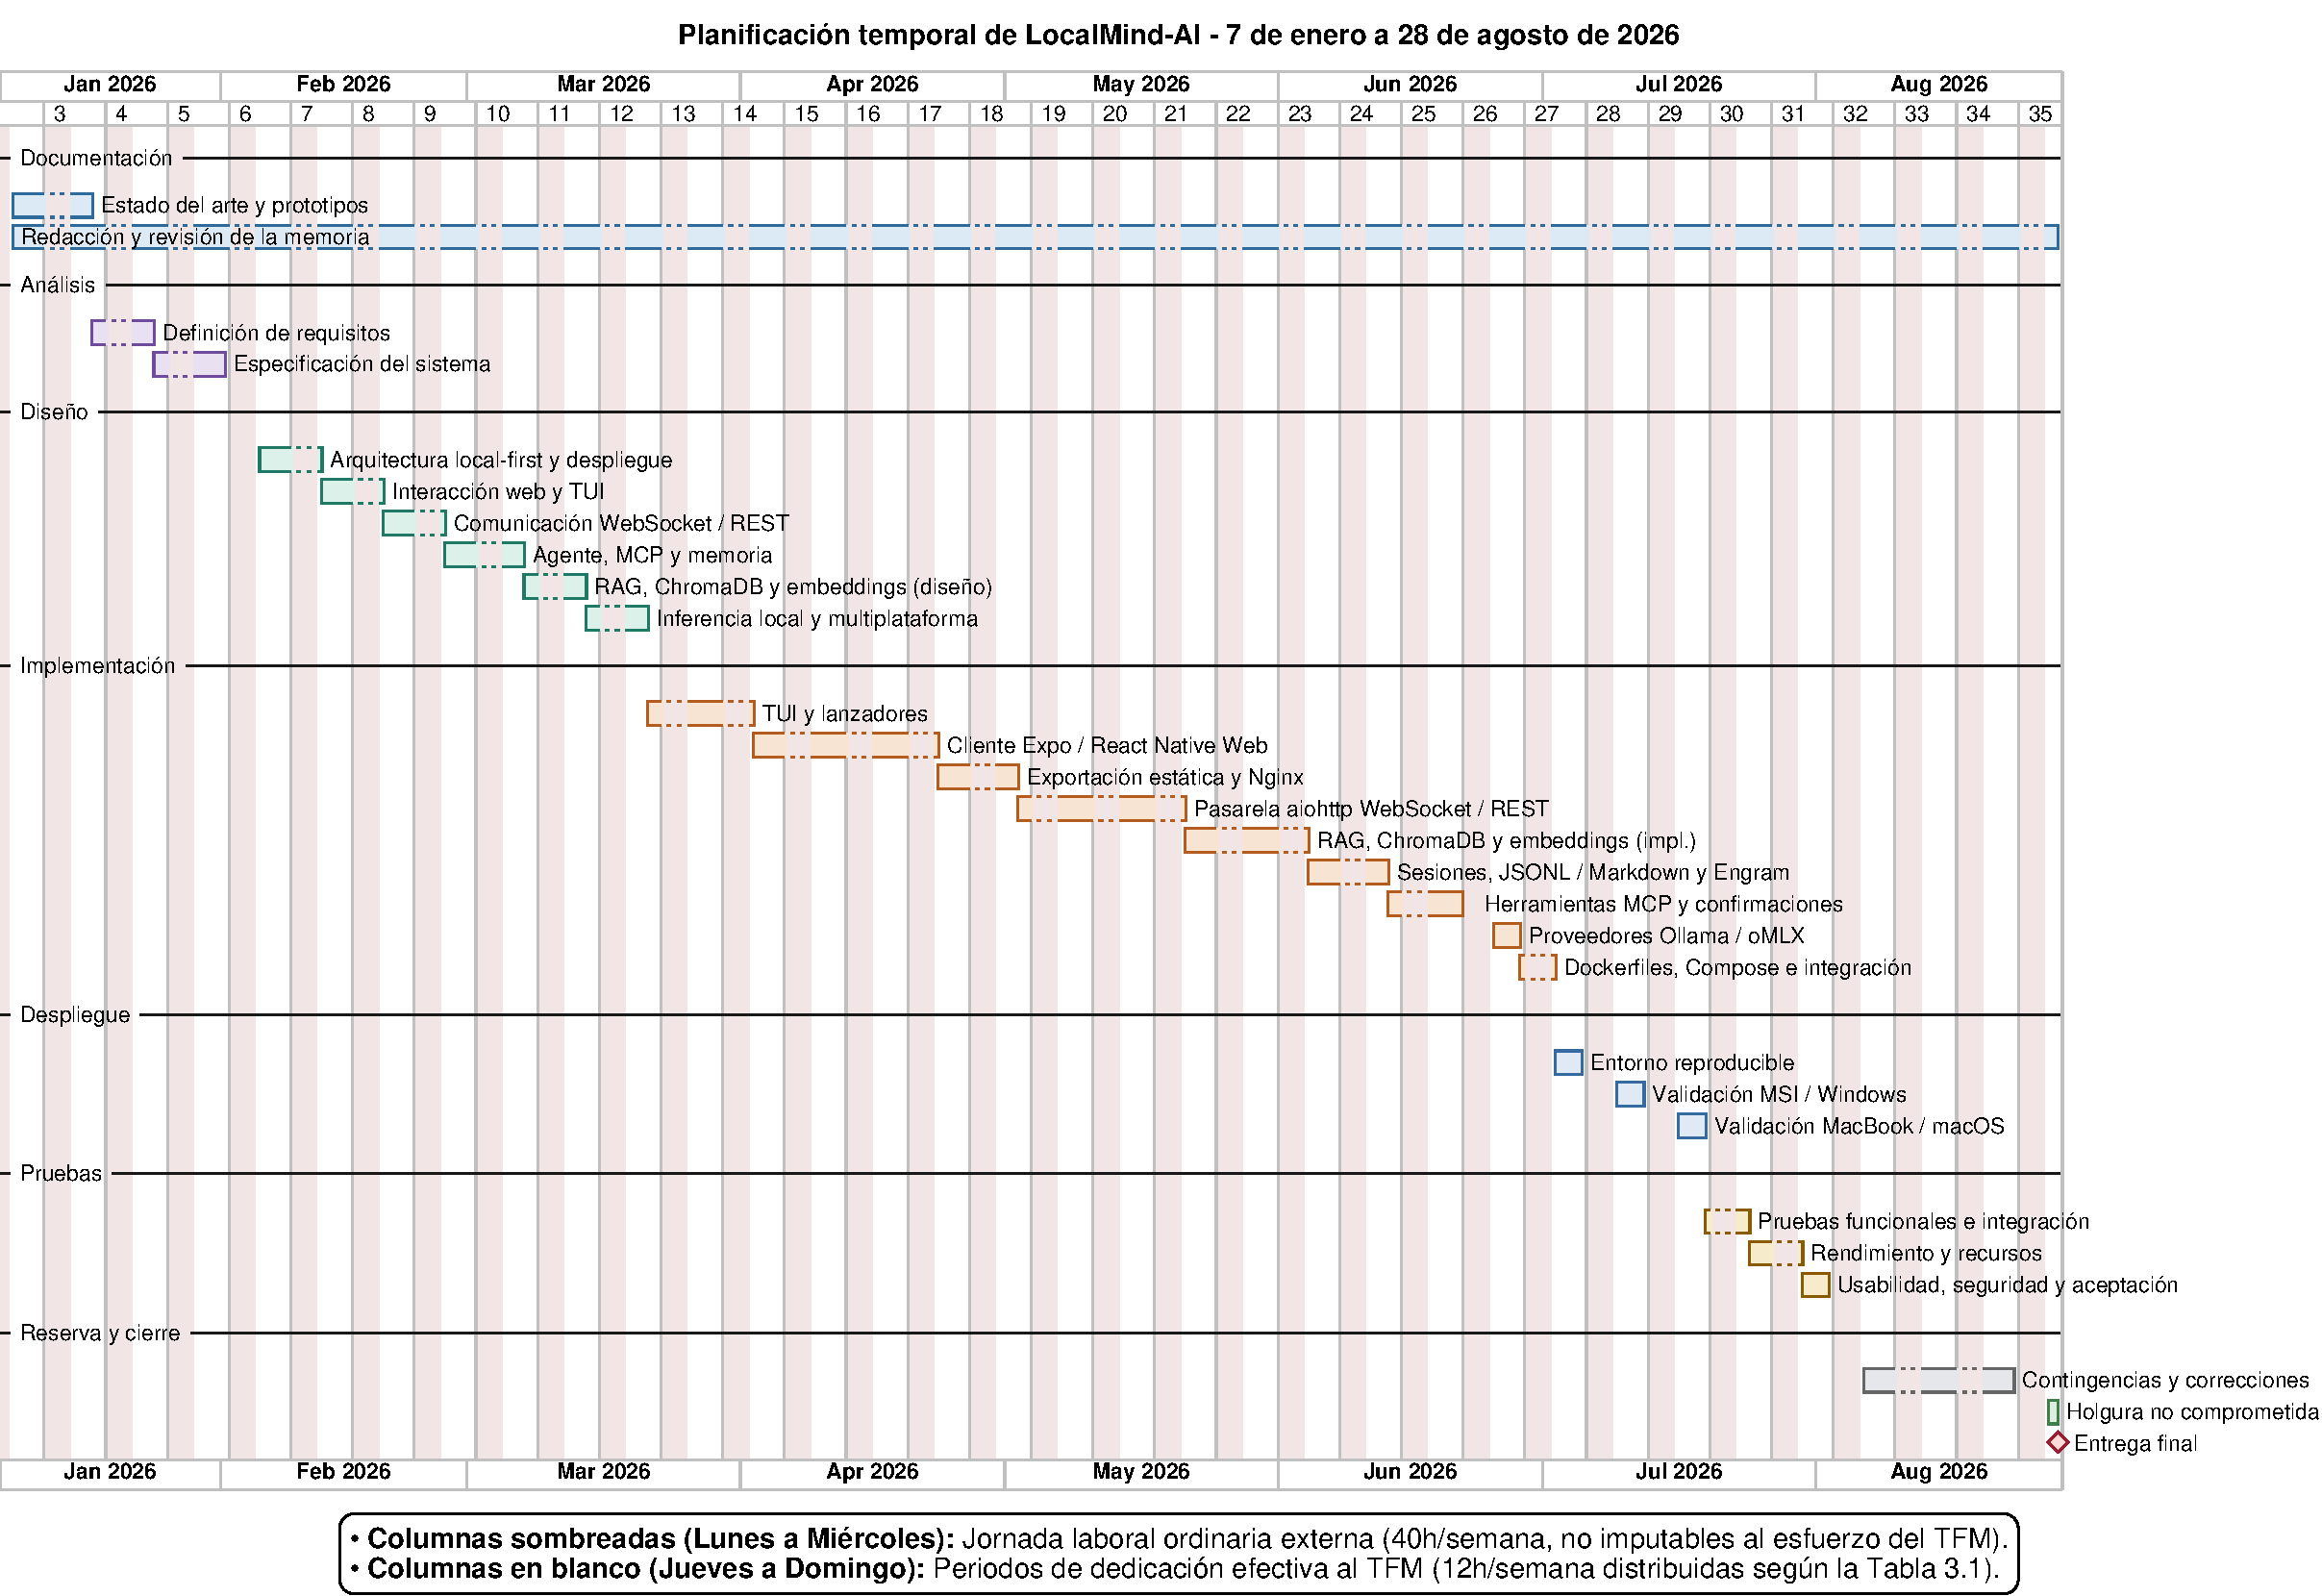
\includegraphics[width=0.98\textheight]{figs/GanttTFM.pdf}
    \caption{Diagrama de Gantt del proyecto, del 7 de enero al 28 de agosto de 2026.}
    \label{fig:diagramaGantt}
\end{sidewaysfigure}

\FloatBarrier

A efectos de estimación económica, el trabajo del autor se valora como el de un perfil \gls{fullstack} júnior. Glassdoor sitúa el salario medio del puesto en España en 22.744~\texteuro{} anuales y publica una equivalencia aproximada de 11~\texteuro{}/hora \cite{SueldoJuniorFull}. Esta tarifa se aplica a las 396 horas presupuestadas, por lo que el salario imputable asciende a 4.356,00~\texteuro{}. Para aproximar el coste empresarial se añade un 33\,\% en concepto de cotizaciones sociales \cite{SeguridadSocialCotizacion}; este porcentaje se utiliza como hipótesis presupuestaria y no como una liquidación laboral individual. El coste total del recurso humano resulta así de 5.793,48~\texteuro{}.

Las herramientas de desarrollo, bibliotecas y servicios utilizados se encuentran disponibles mediante licencias de código abierto, modalidades gratuitas o acceso académico ya disponible. Por ello, se asigna un coste directo de 0,00~\texteuro{} al \gls{software}. La electricidad, la conexión a Internet y los consumibles menores se consideran dentro de los costes indirectos.

Para valorar los equipos se emplea su precio de mercado consultado el 23 de julio de 2026. El MSI Pulse GL66 12UEK-085ES se valora en 917,80~\texteuro{} como equipo reacondicionado \cite{MSIPulseGL66}, mientras que el MacBook Air M4 de 13 pulgadas, con 16~GB de memoria unificada y 512~GB de almacenamiento, se valora en 1.109,00~\texteuro{} \cite{KtuinMacBookAirM4}. El HP OMEN utilizado como referencia descartada en el estado del arte no interviene en la ejecución ni se incorpora al presupuesto.

La tabla simplificada de la \gls{aeat} establece para los equipos informáticos un coeficiente máximo de amortización del 26\,\% y un periodo máximo de diez años \cite{AgenciaTributaria354}. Se adopta una vida útil de cuatro años y se imputa únicamente la fracción correspondiente a los 234 días naturales del proyecto. La Ecuación~\ref{eq:costematerial} formaliza este cálculo.

% Ecuación amortización del material.
\begin{equation}
    A_i = \frac{C_i}{4} \times \frac{234}{365}
    \label{eq:costematerial}
\end{equation}

En la ecuación, \(C_i\) representa el valor de mercado del equipo y \(A_i\) su coste amortizado. Cada amortización se redondea a céntimos antes de calcular los subtotales. La Tabla~\ref{tab:coste_amortizacion} muestra el resultado.

% Tabla de amortización de dispositivos.
\begin{table}[h!tp]
    \centering
    \begin{tabularx}{\textwidth}{|>{\raggedright\arraybackslash}X|>{\centering\arraybackslash}p{2.5cm}|>{\centering\arraybackslash}p{2.3cm}|>{\centering\arraybackslash}p{2.5cm}|}
        \hline
        \textbf{Equipo}                          & \textbf{Valor de mercado} & \textbf{Periodo imputado} & \textbf{Amortización} \\ \hline
        MSI Pulse GL66 12UEK-085ES               & 917,80~\texteuro{}        & 234 días                  & 147,10~\texteuro{}    \\ \hline
        MacBook Air M4 de 13 pulgadas, 16/512~GB & 1.109,00~\texteuro{}      & 234 días                  & 177,74~\texteuro{}    \\ \hline
    \end{tabularx}
    \caption{Valoración y amortización de los equipos utilizados.}
    \label{tab:coste_amortizacion}
\end{table}

Los costes directos se obtienen sumando el recurso humano, la amortización del hardware y el software. Sobre este subtotal se aplica un \textit{overhead} del 20\,\% para cubrir los costes indirectos. Como resume la Tabla~\ref{tab:costos}, el coste estimado del proyecto asciende a 7.341,98~\texteuro{}.

% Tabla de desglose de costes.
\begin{table}[h!tp]
    \centering
    \begin{tabular}{|>{\raggedright\arraybackslash}p{9cm}|>{\centering\arraybackslash}p{3.5cm}|}
        \hline
        \textbf{Concepto}                 & \textbf{Coste}                \\ \hline
        Recursos humanos                  & 5.793,48~\texteuro{}          \\ \hline
        Amortización del MSI Pulse GL66   & 147,10~\texteuro{}            \\ \hline
        Amortización del MacBook Air M4   & 177,74~\texteuro{}            \\ \hline
        Software y servicios              & 0,00~\texteuro{}              \\ \hline
        \textbf{Total de costes directos} & \textbf{6.118,32~\texteuro{}} \\ \hline
        Costes indirectos (20\,\%)        & 1.223,66~\texteuro{}          \\ \hline
        \textbf{Coste total}              & \textbf{7.341,98~\texteuro{}} \\ \hline
    \end{tabular}
    \caption{Desglose de costes del proyecto.}
    \label{tab:costos}
\end{table}

\FloatBarrier

\section{Riesgos}
% Riesgos que pueden afectar al desarrollo del sistema.
El carácter unipersonal del proyecto, su compatibilización con una jornada laboral y la integración de componentes heterogéneos introducen riesgos que pueden alterar la planificación. La Tabla~\ref{tab:risk_analysis} recoge los principales riesgos identificados, su desviación temporal estimada y la respuesta prevista. El coste expresa una demora potencial si se materializa el riesgo, no una reserva que deba añadirse automáticamente a las 396 horas presupuestadas.

\begin{table}[p]
    \centering
    \footnotesize
    \renewcommand{\arraystretch}{1.15}
    \begin{tabularx}{\textwidth}{
            |>{\raggedright\arraybackslash}p{4.2cm}
            |>{\centering\arraybackslash}p{2.1cm}
            |>{\raggedright\arraybackslash}X|
        }
        \hline
        \textbf{Riesgo} & \textbf{Coste}                                                                                                                                                                          & \textbf{Solución} \\ \hline
        Desviación del alcance al compatibilizar el \gls{tfm} con la jornada laboral
                        & Hasta 2 semanas
                        & Mantener cerrado el alcance del producto mínimo viable, revisar semanalmente el trabajo restante y posponer prototipos futuros antes de ampliar el calendario.                                              \\ \hline
        Instalación inconsistente entre \gls{windows} y \gls{macos}
                        & 5 días
                        & Ejecutar instalaciones limpias en el MSI y el MacBook, conservar diagnósticos reproducibles y documentar las diferencias entre \gls{ollama} y \gls{omlx}.                                                   \\ \hline
        Fallos de integración entre el cliente, \gls{nanobot}, \gls{websocket}/\gls{rest}, \gls{mcp}, \gls{rag} y la memoria
                        & 5 días
                        & Definir pruebas de contrato para cada frontera, integrar de forma incremental y conservar registros que permitan aislar el componente responsable.                                                          \\ \hline
        Recursos insuficientes o rendimiento inadecuado de los modelos
                        & 5 días
                        & Medir memoria y latencia por equipo, reducir contexto o cuantización y disponer de modelos alternativos de menor tamaño compatibles con el motor activo.                                                    \\ \hline
        Exposición de datos, credenciales o servicios locales
                        & 4 días
                        & Enlazar los servicios a la interfaz de bucle local, mantener los secretos fuera del código y solicitar confirmación antes de ejecutar acciones protegidas o activar servicios externos.                     \\ \hline
        Pérdida o corrupción de sesiones, memoria o colección vectorial
                        & 3 días
                        & Verificar los volúmenes persistentes, realizar copias de seguridad de los almacenes y probar su restauración antes de las validaciones finales.                                                             \\ \hline
        Cambios incompatibles en dependencias, modelos, interfaces o licencias
                        & 4 días
                        & Fijar versiones e identificadores, revisar las notas de publicación y mantener una alternativa conocida para cada dependencia crítica.                                                                      \\ \hline
    \end{tabularx}
    \caption{Análisis de riesgos, costes temporales y medidas de contingencia.}
    \label{tab:risk_analysis}
\end{table}

Las desviaciones de la tabla representan escenarios alternativos y, por tanto, no deben sumarse entre sí como si todos fueran a producirse. Si coincidieran varios riesgos graves y se agotara el margen previsto, se reduciría primero el alcance no esencial para preservar los requisitos del prototipo académico y la fecha de entrega.

\FloatBarrier

\section{Viabilidad}
% Viabilidad del proyecto presentado.
La viabilidad económica del proyecto es favorable dentro de su alcance académico. El coste estimado de 7.341,98~\texteuro{} incluye la valoración del trabajo y la amortización de los dos equipos, aunque no exige adquirirlos expresamente porque ambos se reutilizan. El coste directo de software y servicios se mantiene en 0,00~\texteuro{}, al emplearse soluciones de código abierto, gratuitas o disponibles mediante acceso académico.

Desde el punto de vista temporal, las 396 horas presupuestadas caben dentro de las 400 horas que proporciona el calendario. Sin embargo, la diferencia de cuatro horas es reducida y hace necesario controlar el alcance y aplicar las medidas de contingencia en cuanto se detecte una desviación. La duración total, superior a siete meses, no responde a una carga de trabajo a tiempo completo, sino a la dedicación de doce horas semanales compatible con una jornada laboral ordinaria de ocho horas diarias.

La viabilidad organizativa se encuentra condicionada por el desarrollo unipersonal. Esta configuración reduce el coste y facilita mantener una visión coherente del sistema, pero impide paralelizar actividades críticas y limita la revisión cruzada de decisiones. Para compensarlo, el proyecto se divide en incrementos verificables y reserva periodos específicos para validación, contingencias y correcciones.

La solución es técnicamente viable porque se apoya en tecnologías compatibles con la arquitectura descrita: un cliente web estático servido por \gls{nginx}, un agente \gls{nanobot} contenerizado, comunicación directa mediante \gls{websocket} y \gls{rest}, y motores de inferencia nativos \gls{ollama} u \gls{omlx}. No obstante, la viabilidad completa depende todavía de demostrar la instalación multiplataforma, el consumo de recursos, la persistencia, la observabilidad y las medidas de seguridad definidas en los requisitos.

La viabilidad operativa exige disponer de \gls{docker}, de un motor de inferencia compatible y de memoria suficiente para el modelo seleccionado. Una vez instaladas las dependencias y descargados los modelos, las funciones locales previstas deberán poder utilizarse sin conexión. Las integraciones externas no son necesarias para el funcionamiento básico y deben permanecer deshabilitadas hasta que exista una activación consciente.

En consecuencia, LocalMind-AI se considera viable como prototipo académico y personal, siempre que se mantenga el alcance definido y se completen las validaciones pendientes. Esta conclusión no equivale a afirmar que todos los objetivos de rendimiento, seguridad o compatibilidad se encuentren ya demostrados.

\subsection{Viabilidad legal}

El tratamiento de información en LocalMind-AI debe respetar el \gls{rgpd}, establecido por el Reglamento (UE) 2016/679 \cite{ReglamentoUE20162016}, y la \gls{lopdgdd}, que complementa este marco en España \cite{BOEA201816673LeyOrganica}. El enfoque local reduce transferencias innecesarias, pero no garantiza por sí solo el cumplimiento: siguen siendo necesarias la minimización de datos, la protección de credenciales, el control de los almacenes persistentes y la posibilidad de eliminar la información.

Las pruebas y demostraciones del \gls{tfm} utilizarán exclusivamente datos públicos o sintéticos. Si se habilita una herramienta o un proveedor externo, la persona usuaria deberá conocer y autorizar la transmisión antes de que se produzca. Esta cautela afecta también a \gls{engram}: la implementación configurada almacena la memoria en una base de datos local, pero su documentación contempla llamadas a un proveedor para \glspl{embeddings} y consolidación, con Gemini como opción predeterminada \cite{engramSdk2026}. Por ello, no se considera completamente desconectado hasta que su configuración concreta haya sido verificada.

El marco europeo aplicable a la \gls{ia} se encuentra en el Reglamento (UE) 2024/1689, denominado \gls{aiact}, cuya aplicación general comienza el 2 de agosto de 2026, sin perjuicio de las fechas específicas previstas para determinadas disposiciones \cite{ReglamentoUE20241689}. El prototipo deberá facilitar la supervisión humana, diferenciar las respuestas generadas y solicitar confirmación para acciones protegidas. No obstante, esta memoria no asigna al sistema una categoría jurídica definitiva de riesgo, ya que dicha clasificación depende del contexto de uso y de una evaluación legal que excede el alcance técnico del trabajo.

LocalMind-AI se presenta al cierre del \gls{tfm} como un prototipo académico y personal, sin distribución pública ni explotación comercial. El directorio raíz del proyecto no declara todavía una licencia propia, por lo que no debe interpretarse la disponibilidad local del código como una autorización de redistribución. Antes de una publicación futura sería necesario elegir una licencia compatible, conservar los avisos de terceros y revisar las condiciones de los modelos y de los servicios empleados.

La Tabla~\ref{tab:licencias} resume las licencias principales. Cuando un producto combina código abierto con una distribución o un servicio sujeto a términos adicionales, ambas condiciones se distinguen expresamente.

% Tabla de licencias tecnológicas.
\begin{table}[p]
    \centering
    \scriptsize
    \renewcommand{\arraystretch}{1.15}
    \begin{tabularx}{\textwidth}{
            |>{\raggedright\arraybackslash}p{3.6cm}
            |>{\raggedright\arraybackslash}p{3.1cm}
            |>{\raggedright\arraybackslash}X|
        }
        \hline
        \textbf{Software o recurso} & \textbf{Licencia o condiciones}                                                                                                                                                                                                                                                                                              & \textbf{Observaciones} \\ \hline
        \Gls{nanobot}, \gls{mcp}, \gls{aiohttp} y \gls{python}
                                    & \gls{mit}, \gls{apache2.0} y \gls{psfl}
                                    & Nanobot y el SDK de MCP se distribuyen bajo MIT, aiohttp bajo Apache 2.0 y Python bajo PSFL \cite{nanobot2026,mcpPythonSdk2026,aiohttpLicense2026,pythonLicense2026}.                                                                                                                                                                                 \\ \hline
        React, \gls{reactnative}, \gls{expo}, \gls{nodejs} y \gls{pnpm}
                                    & \gls{mit}
                                    & Los componentes de este grupo declaran licencias MIT en sus repositorios oficiales \cite{react2026,meta2024reactnative,expo2024,nodejs2026,pnpm2026}.                                                                                                                                                                                                 \\ \hline
        Docker Engine/Compose, Docker Desktop y \gls{nginx}
                                    & \gls{apache2.0}, términos de suscripción y \gls{bsd2}
                                    & Engine y Compose son proyectos Apache 2.0, Docker Desktop está sujeto a términos propios y Nginx utiliza BSD-2-Clause \cite{dockerEngineLicense2026,dockerComposeLicense2026,dockerDesktopTerms2026,nginxLicense2026}.                                                                                                                                \\ \hline
        \Gls{ollama}, \gls{mlx} y \gls{omlx}
                                    & \gls{mit} y \gls{apache2.0}
                                    & Ollama y MLX declaran MIT, mientras que oMLX declara Apache 2.0 \cite{ollamaLicense2026,mlxLicense2026,omlx2026}.                                                                                                                                                                                                                                     \\ \hline
        \Gls{chromadb} y Engram SDK
                                    & \gls{apache2.0} y \gls{mit}
                                    & ChromaDB declara Apache 2.0 y el paquete \texttt{engram-sdk} MIT, el cual puede utilizar proveedores externos según su configuración \cite{chroma2026,engramSdk2026}.                                                                                                                                                                                 \\ \hline
        Ornith-1.0-9B (4-bit / 6-bit), Qwen3.5-9B-Instruct (4-bit / 6-bit), Qwopus3.5-9B-Coder (4-bit / 6-bit) y Qwopus3.5-4B-Coder (4-bit / 6-bit)
                                    & \gls{mit} y \gls{apache2.0}
                                    & Las versiones cuantizadas de Ornith-1.0-9B en 4 y 6 bits declaran MIT en HuggingFace, mientras que los modelos Qwen3.5-9B-Instruct y Qwopus3.5-Coder en sus variantes de 9B y 4B parámetros con cuantizaciones de 4 y 6 bits o esquemas Q4\_K\_M y Q6\_K se distribuyen bajo Apache 2.0 \cite{ornith9b4,ornith9b6,qwen359b}.                          \\ \hline
        \Gls{git} y GitHub
                                    & \gls{gpl2only} y términos de servicio
                                    & Git se distribuye bajo GPL-2.0-only, mientras que el alojamiento y las funciones de GitHub se rigen por sus condiciones de servicio \cite{gitLicense2026,githubTerms2026}.                                                                                                                                                                            \\ \hline
        \Gls{latex}, \gls{mactex} y \gls{plantuml}
                                    & \gls{lppl}, licencias múltiples y \gls{gnugpl3}
                                    & LaTeX utiliza LPPL, MacTeX agrupa componentes con licencias propias y PlantUML se distribuye bajo GPL v3 \cite{latexLicense2026,mactex2026,plantumlLicense2026}.                                                                                                                                                                                      \\ \hline
        Zotero, Visual Studio Code y Visual Paradigm
                                    & \gls{agpl3}, MIT o propietaria y propietaria académica
                                    & Zotero declara AGPL v3, Code-OSS es MIT, la distribución de Microsoft se rige por su licencia de producto y Visual Paradigm utiliza condiciones propietarias para su edición académica \cite{zoteroLicense2026,vscodeLicense2026,VisualParadigmLicensing}.                                                                                            \\ \hline
    \end{tabularx}
    \caption{Licencias y condiciones de las tecnologías empleadas.}
    \label{tab:licencias}
\end{table}

\FloatBarrier


\chapter{Análisis}\label{ch:analisis}
% Capítulo 4 — Análisis del Sistema (LocalMind-AI)
% Reescrito para el TFM; contenido original (no se reutiliza prosa del TFG).

Este capítulo presenta el análisis del sistema LocalMind-AI a partir de los requisitos identificados en el Capítulo~\ref{ch:requisitos}. El propósito es describir las interacciones entre la persona usuaria y el \gls{nanobot}, modeladas mediante casos de uso, diagramas de secuencia, de clases y de actividades siguiendo la especificación estándar de la Open Management Group \cite{omgUml2024} y la metodología de análisis orientado a objetos \cite{larmanIterativeIncrementalDevelopments2003}. El análisis se articula en torno a un único actor, la persona usuaria, que accede al sistema principalmente a través de una interfaz web desarrollada en Expo y React Native Web conectada mediante \gls{websocket}, contando con la \gls{tui} en Python y Rich para tareas de instalación, configuración y diagnóstico en entorno local.

El sistema LocalMind-AI es un asistente de \gls{ia} orientado a la ejecución local que combina razonamiento \gls{cot} con recuperación aumentada por generación mediante el protocolo \gls{cotrag}, apoyándose en herramientas externas a través del protocolo \gls{mcp}. Los motores de inferencia (\gls{ollama} y \gls{omlx}) y la base de conocimiento vectorial (\gls{chromadb}) operan íntegramente en el equipo de la persona usuaria, garantizando la privacidad de los datos descrita en el requisito no funcional RNF1.

\section{Diagrama de casos de uso}

La Figura~\ref{fig:diagramaCU} recoge los nueve casos de uso que cubren la totalidad de los requisitos funcionales (RF1 a RF10) y no funcionales (RNF1 a RNF14) definidos en el Capítulo~\ref{ch:requisitos}. El actor único es la persona usuaria, que interactúa con el sistema a través de la interfaz web o la \gls{tui}, conectadas mediante \gls{websocket} al puerto 8765 o mediante la API REST en el puerto 8900 del \gls{nanobot}.

\begin{figure}[h!tp]
  \centering
  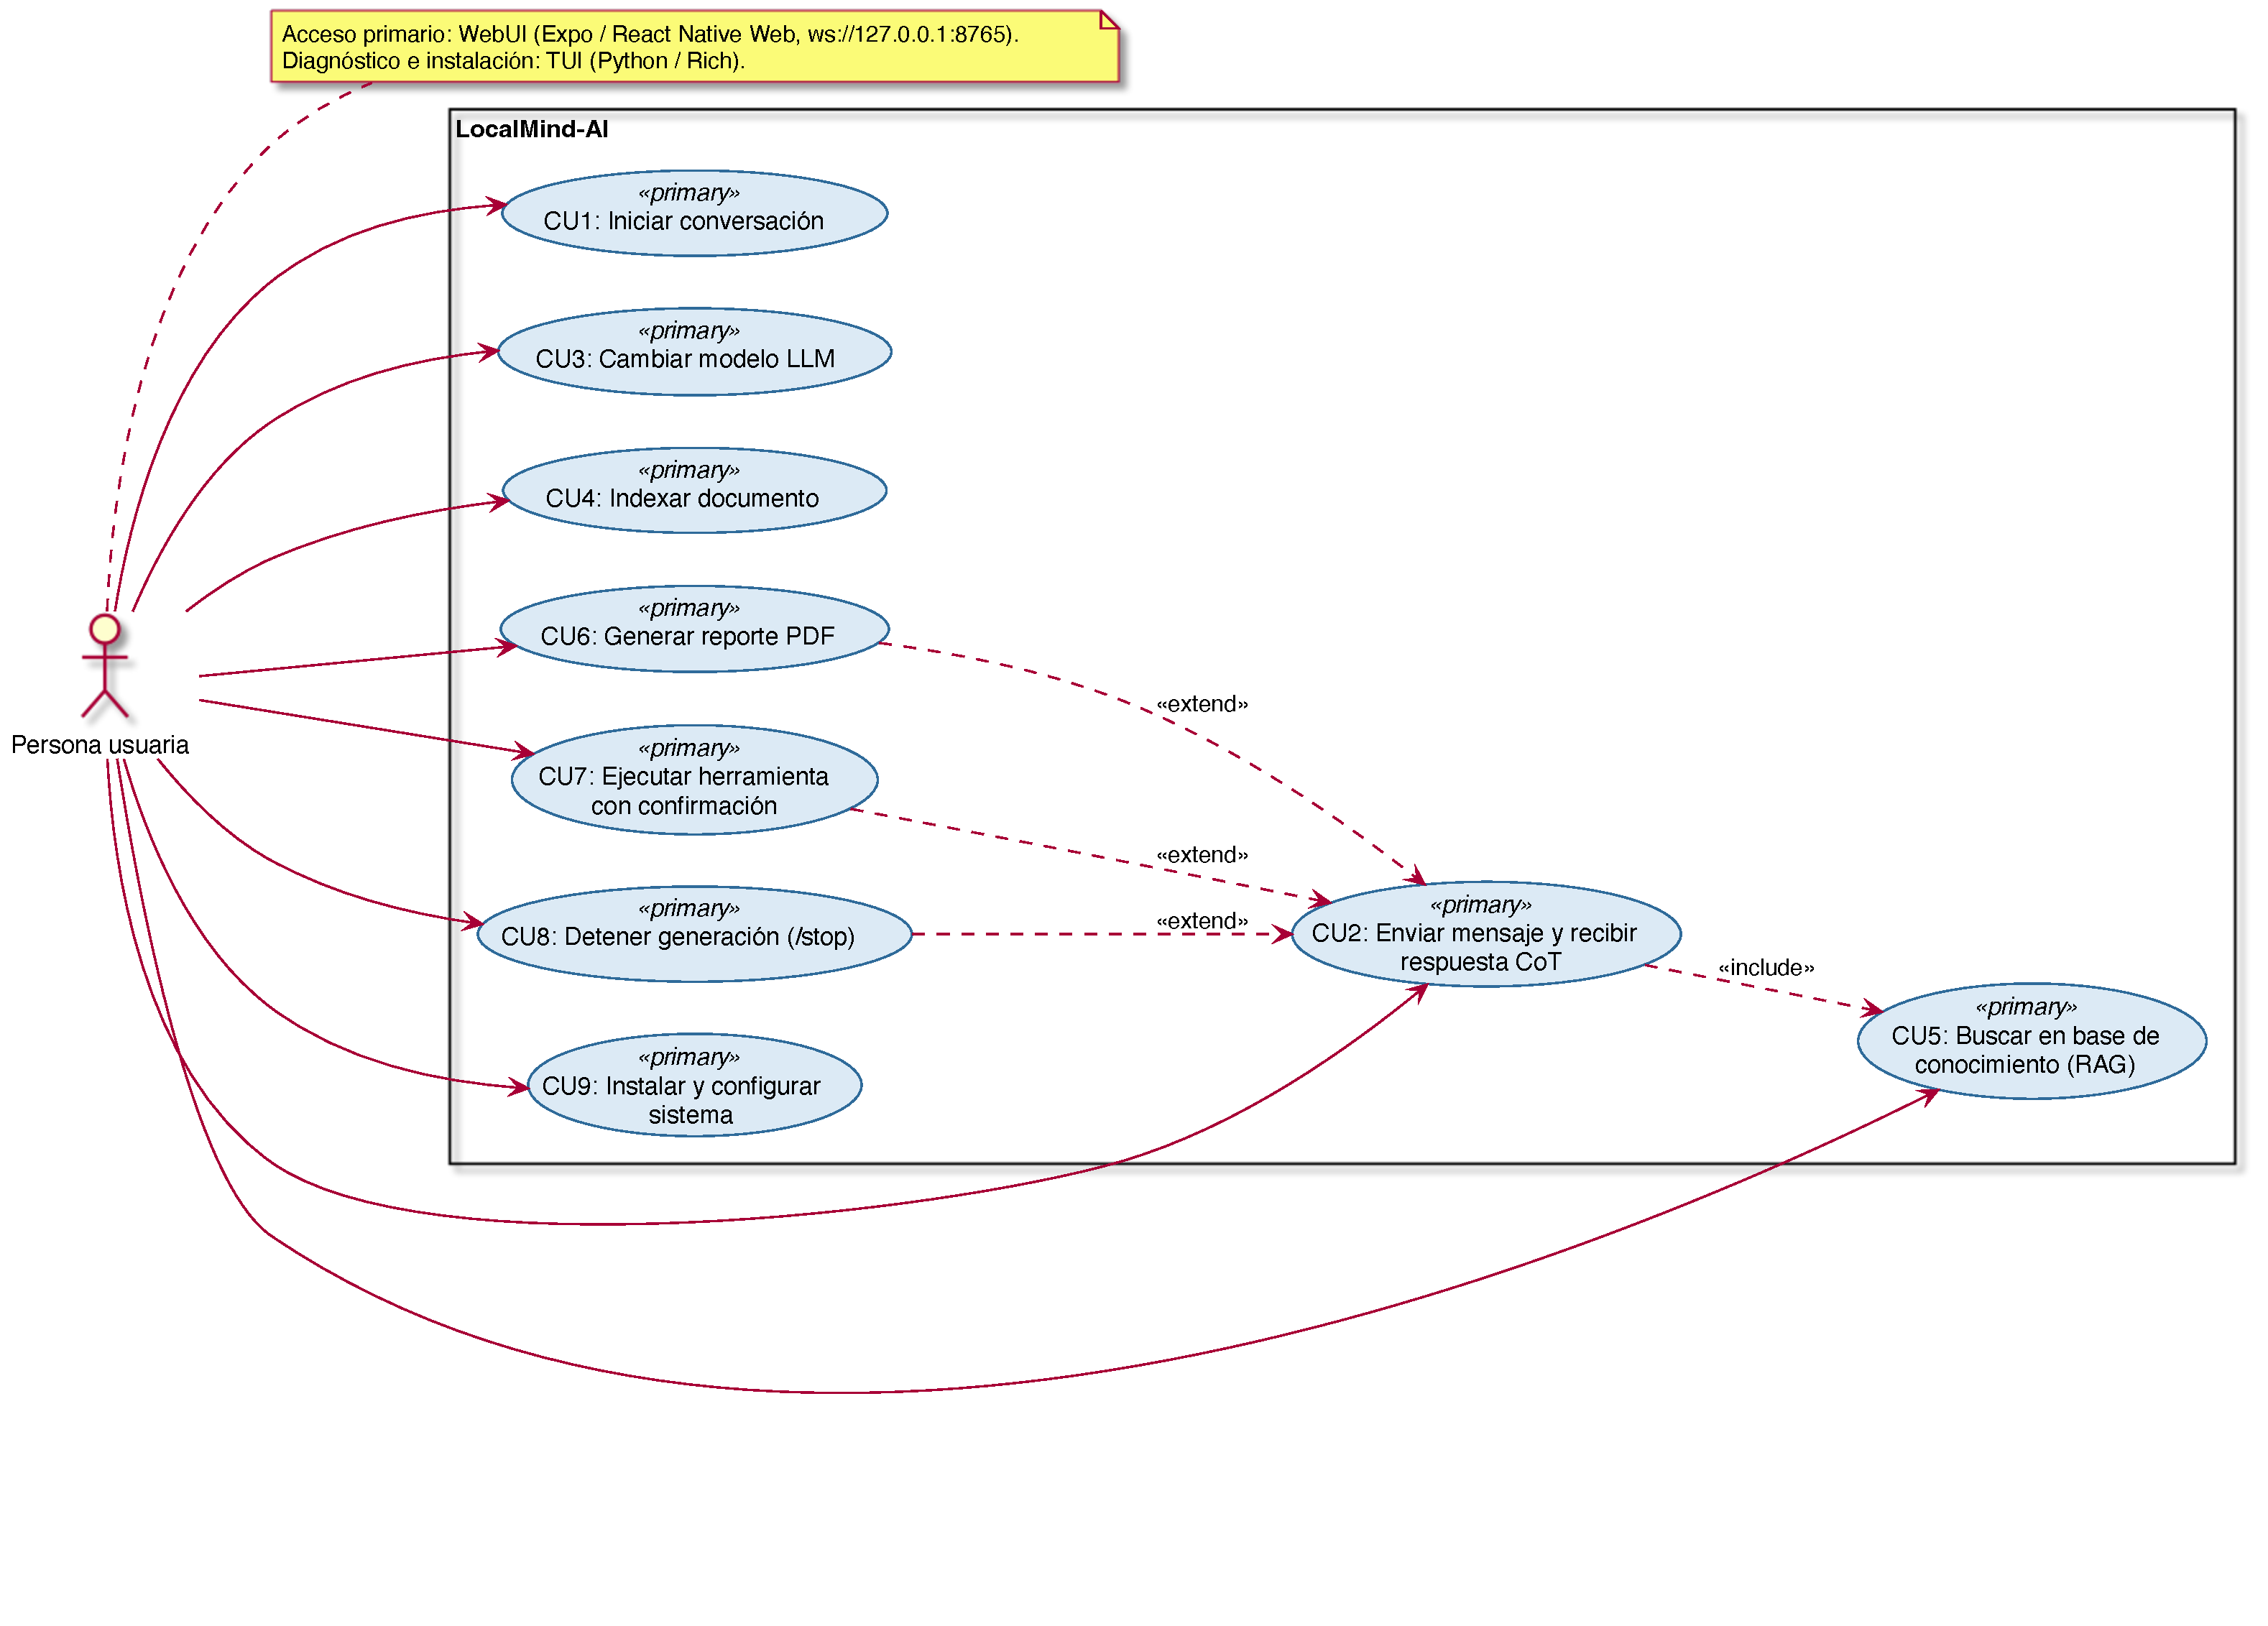
\includegraphics[width=0.9\textwidth]{figs/diagrama-casos-uso.pdf}
  \caption{Diagrama de casos de uso de LocalMind-AI.}
  \label{fig:diagramaCU}
\end{figure}

A continuación se detallan los nueve casos de uso del sistema. Cada tabla presenta las ocho secciones descriptivas estandarizadas \cite{omgUml2024} con el identificador, nombre, actores, descripción, flujo de datos principal, precondiciones, postcondiciones y requisitos asociados.

% Caso de Uso 1.
\begin{table}[h!tp]
  \centering
  \begin{adjustbox}{max width=\textwidth}
    \begin{tabular}{|>{\centering\arraybackslash}p{3cm}|p{8.5cm}|}
      \hline
      \textbf{Caso de Uso}      & CU1 \\ \hline
      \textbf{Nombre}           & Iniciar conversación \\ \hline
      \textbf{Actores}          & Persona usuaria (a través de WebUI o TUI) \\ \hline
      \textbf{Descripción}      & Establece una sesión conversacional con el sistema. El cliente abre un canal de comunicación con el \gls{nanobot} y crea un contexto de sesión persistente con identificador único. \\ \hline
      \textbf{Flujo de datos}   &
      \begin{minipage}[t]{\linewidth}
        \vspace{0.4em}
        \begin{enumerate}[leftmargin=*,noitemsep,topsep=2pt]
          \item La persona usuaria abre la aplicación cliente en la WebUI o en la TUI.
          \item El cliente establece la conexión \gls{websocket} al puerto 8765 o realiza una petición a la API REST.
          \item El componente \texttt{WebSocketChannel} acepta la conexión y notifica al gestor de canales.
          \item El componente \texttt{AgentLoop} genera una nueva sesión con su identificador único.
          \item Se inicializa el archivo de sesión \gls{jsonl} en el volumen de almacenamiento persistente.
          \item El cliente recibe la confirmación de sesión activa y lista para recibir entradas.
        \end{enumerate}
        \vspace{0.4em}
      \end{minipage} \\ \hline
      \textbf{Precondiciones}   & Los servicios del contenedor están en ejecución y el motor de inferencia local es accesible. \\ \hline
      \textbf{Postcondiciones}  & Sesión creada con identificador único, historial \gls{jsonl} inicializado y canal en estado activo. \\ \hline
      \textbf{Requisitos}       & RF1, RF2, RF8, RNF1, RNF4, RNF7 \\ \hline
    \end{tabular}
  \end{adjustbox}
  \caption{CU1. Iniciar conversación.}
  \label{tab:CU1}
\end{table}

% Caso de Uso 2.
\begin{table}[h!tp]
  \centering
  \begin{adjustbox}{max width=\textwidth}
    \begin{tabular}{|>{\centering\arraybackslash}p{3cm}|p{8.5cm}|}
      \hline
      \textbf{Caso de Uso}      & CU2 \\ \hline
      \textbf{Nombre}           & Enviar mensaje y recibir respuesta en streaming CoT \\ \hline
      \textbf{Actores}          & Persona usuaria (a través de WebUI o TUI) \\ \hline
      \textbf{Descripción}      & La persona usuaria envía un mensaje de texto y recibe la respuesta del \gls{llm} en fragmentos incrementales mediante emisión continua, con visibilidad de los pasos intermedios del razonamiento \gls{cotrag}. \\ \hline
      \textbf{Flujo de datos}   &
      \begin{minipage}[t]{\linewidth}
        \vspace{0.4em}
        \begin{enumerate}[leftmargin=*,noitemsep,topsep=2pt]
          \item La persona usuaria escribe y envía un mensaje de texto.
          \item El cliente transmite el mensaje \texttt{new\_chat} a través del canal \gls{websocket}.
          \item El componente \texttt{WebSocketChannel} recibe el mensaje y lo publica en la barra de eventos.
          \item El método de procesamiento del agente invoca al constructor de contexto para enriquecer la solicitud con el historial, la memoria y los documentos recuperados.
          \item El ejecutor del agente invoca al proveedor del modelo con el contexto construido.
          \item El proveedor consulta al motor de inferencia seleccionado.
          \item El motor genera tokens de forma incremental.
          \item Cada token se envía como un paquete incremental al cliente mediante \gls{websocket}.
          \item Al recibir el token de finalización, se emite el evento de cierre y se guarda la respuesta en el archivo de sesión.
        \end{enumerate}
        \vspace{0.4em}
      \end{minipage} \\ \hline
      \textbf{Precondiciones}   & Sesión activa iniciada previamente en el caso de uso CU1 y canal de comunicación operativo. \\ \hline
      \textbf{Postcondiciones}  & Respuesta completa almacenada en el historial y renderizada correctamente en el cliente. \\ \hline
      \textbf{Requisitos}       & RF1, RF2, RF10, RNF2, RNF3, RNF7 \\ \hline
    \end{tabular}
  \end{adjustbox}
  \caption{CU2. Enviar mensaje y recibir respuesta en streaming CoT.}
  \label{tab:CU2}
\end{table}

% Caso de Uso 3.
\begin{table}[h!tp]
  \centering
  \begin{adjustbox}{max width=\textwidth}
    \begin{tabular}{|>{\centering\arraybackslash}p{3cm}|p{8.5cm}|}
      \hline
      \textbf{Caso de Uso}      & CU3 \\ \hline
      \textbf{Nombre}           & Cambiar modelo LLM \\ \hline
      \textbf{Actores}          & Persona usuaria (a través de WebUI o TUI) \\ \hline
      \textbf{Descripción}      & La persona usuaria alterna dinámicamente entre \gls{ollama} y \gls{omlx} como motor de inferencia activo, o cambia la variante del modelo sin necesidad de reiniciar la sesión. \\ \hline
      \textbf{Flujo de datos}   &
      \begin{minipage}[t]{\linewidth}
        \vspace{0.4em}
        \begin{enumerate}[leftmargin=*,noitemsep,topsep=2pt]
          \item La persona usuaria accede al panel de selección de modelos en la interfaz.
          \item Selecciona el motor de inferencia objetivo y la variante de cuantización deseada.
          \item El cliente envía la solicitud de cambio de proveedor al agente.
          \item El bucle del agente actualiza la instancia del proveedor de \gls{llm} con el nuevo motor.
          \item Se realiza una prueba de conectividad con el nuevo proveedor.
          \item Se notifica la confirmación del cambio al cliente.
        \end{enumerate}
        \vspace{0.4em}
      \end{minipage} \\ \hline
      \textbf{Precondiciones}   & Al menos un motor de inferencia local en ejecución y accesible durante una sesión activa. \\ \hline
      \textbf{Postcondiciones}  & Proveedor reconfigurado para que las siguientes peticiones empleen el nuevo motor seleccionado. \\ \hline
      \textbf{Requisitos}       & RF3, RNF4, RNF9 \\ \hline
    \end{tabular}
  \end{adjustbox}
  \caption{CU3. Cambiar modelo \gls{llm}.}
  \label{tab:CU3}
\end{table}

% Caso de Uso 4.
\begin{table}[h!tp]
  \centering
  \begin{adjustbox}{max width=\textwidth}
    \begin{tabular}{|>{\centering\arraybackslash}p{3cm}|p{8.5cm}|}
      \hline
      \textbf{Caso de Uso}      & CU4 \\ \hline
      \textbf{Nombre}           & Indexar documento en base de conocimiento \\ \hline
      \textbf{Actores}          & Persona usuaria (a través de WebUI) \\ \hline
      \textbf{Descripción}      & La persona usuaria sube un archivo en formato \gls{pdf} o \gls{markdown} que se procesa, se trocea en fragmentos semánticos y se indexa como vectores en \gls{chromadb}. \\ \hline
      \textbf{Flujo de datos}   &
      \begin{minipage}[t]{\linewidth}
        \vspace{0.4em}
        \begin{enumerate}[leftmargin=*,noitemsep,topsep=2pt]
          \item La persona usuaria selecciona un documento en formato \gls{pdf} o \gls{markdown}.
          \item El cliente envía el archivo al servicio a través del punto de entrada de carga.
          \item El agente extrae el contenido textual del archivo recibido.
          \item Se fragmenta el texto mediante división recursiva con solapamiento semántico.
          \item La función de vectorización genera los vectores correspondientes utilizando el servicio local.
          \item Los fragmentos y sus vectores se insertan en la colección de \gls{chromadb}.
          \item Se notifica la finalización indicando el recuento de fragmentos indexados.
        \end{enumerate}
        \vspace{0.4em}
      \end{minipage} \\ \hline
      \textbf{Precondiciones}   & Base de datos vectorial \gls{chromadb} accesible y servicio local de vectorización activo. \\ \hline
      \textbf{Postcondiciones}  & Documento fragmentado e indexado en la base vectorial para consultas futuras. \\ \hline
      \textbf{Requisitos}       & RF4, RF5, RNF5, RNF12 \\ \hline
    \end{tabular}
  \end{adjustbox}
  \caption{CU4. Indexar documento en base de conocimiento.}
  \label{tab:CU4}
\end{table}

% Caso de Uso 5.
\begin{table}[h!tp]
  \centering
  \begin{adjustbox}{max width=\textwidth}
    \begin{tabular}{|>{\centering\arraybackslash}p{3cm}|p{8.5cm}|}
      \hline
      \textbf{Caso de Uso}      & CU5 \\ \hline
      \textbf{Nombre}           & Buscar en base de conocimiento (RAG) \\ \hline
      \textbf{Actores}          & Persona usuaria (a través de WebUI) o invocado por CU2 \\ \hline
      \textbf{Descripción}      & Transforma la consulta en un vector, recupera los fragmentos más afines de la base vectorial \gls{chromadb} e inyecta dicho contexto en la solicitud al \gls{llm}. \\ \hline
      \textbf{Flujo de datos}   &
      \begin{minipage}[t]{\linewidth}
        \vspace{0.4em}
        \begin{enumerate}[leftmargin=*,noitemsep,topsep=2pt]
          \item Se recibe una consulta directa o procedente del flujo \gls{cotrag} en el caso de uso CU2.
          \item El constructor de contexto convierte la consulta en vector mediante la función de vectorización local.
          \item Se consulta la colección de \gls{chromadb} extrayendo los fragmentos más próximos.
          \item Se aplican los filtros correspondientes por umbral de similitud semántica.
          \item Los fragmentos seleccionados se inyectan en el contexto de la solicitud.
          \item El modelo genera la respuesta fundamentada en la información recuperada.
        \end{enumerate}
        \vspace{0.4em}
      \end{minipage} \\ \hline
      \textbf{Precondiciones}   & Al menos un documento indexado en \gls{chromadb} y servicio de vectorización disponible. \\ \hline
      \textbf{Postcondiciones}  & Contexto relevante inyectado en la sesión para la generación de la respuesta. \\ \hline
      \textbf{Requisitos}       & RF5, RNF6, RNF12, RNF14 \\ \hline
    \end{tabular}
  \end{adjustbox}
  \caption{CU5. Buscar en base de conocimiento (\gls{rag}).}
  \label{tab:CU5}
\end{table}

% Caso de Uso 6.
\begin{table}[h!tp]
  \centering
  \begin{adjustbox}{max width=\textwidth}
    \begin{tabular}{|>{\centering\arraybackslash}p{3cm}|p{8.5cm}|}
      \hline
      \textbf{Caso de Uso}      & CU6 \\ \hline
      \textbf{Nombre}           & Generar reporte PDF \\ \hline
      \textbf{Actores}          & Persona usuaria (a través del agente) \\ \hline
      \textbf{Descripción}      & El agente ejecuta la herramienta \gls{mcp} encargada de generar informes para confeccionar un documento en formato \gls{pdf} a partir del contenido de la sesión. \\ \hline
      \textbf{Flujo de datos}   &
      \begin{minipage}[t]{\linewidth}
        \vspace{0.4em}
        \begin{enumerate}[leftmargin=*,noitemsep,topsep=2pt]
          \item El \gls{llm} determina la necesidad de generar un documento y emite una llamada a herramienta.
          \item El ejecutor del agente captura la llamada y consulta el registro de herramientas.
          \item El registro redirige la petición al servidor de herramientas \gls{mcp}.
          \item El servidor ejecuta la función de generación mediante un subproceso conectado por entrada y salida estándar.
          \item El archivo en formato \gls{pdf} se guarda en el espacio de trabajo local persistente.
          \item Se devuelve la confirmación y la ruta del archivo al agente para informar a la persona usuaria.
        \end{enumerate}
        \vspace{0.4em}
      \end{minipage} \\ \hline
      \textbf{Precondiciones}   & Servidor de herramientas \gls{mcp} activo y herramienta registrada correctamente. \\ \hline
      \textbf{Postcondiciones}  & Documento en formato \gls{pdf} creado y almacenado localmente en el directorio de trabajo. \\ \hline
      \textbf{Requisitos}       & RF9, RF10, RNF6, RNF11 \\ \hline
    \end{tabular}
  \end{adjustbox}
  \caption{CU6. Generar reporte \gls{pdf}.}
  \label{tab:CU6}
\end{table}

% Caso de Uso 7.
\begin{table}[h!tp]
  \centering
  \begin{adjustbox}{max width=\textwidth}
    \begin{tabular}{|>{\centering\arraybackslash}p{3cm}|p{8.5cm}|}
      \hline
      \textbf{Caso de Uso}      & CU7 \\ \hline
      \textbf{Nombre}           & Ejecutar herramienta con confirmación \\ \hline
      \textbf{Actores}          & Persona usuaria (a través de WebUI o TUI) \\ \hline
      \textbf{Descripción}      & El agente solicita ejecutar una acción sensible o protegida mediante \gls{mcp}, requiriendo la autorización explícita de la persona usuaria antes de su ejecución. \\ \hline
      \textbf{Flujo de datos}   &
      \begin{minipage}[t]{\linewidth}
        \vspace{0.4em}
        \begin{enumerate}[leftmargin=*,noitemsep,topsep=2pt]
          \item El modelo emite una orden de ejecución de herramienta clasificada como protegida.
          \item El ejecutor del agente detecta la política de confirmación e interrumpe el flujo.
          \item El cliente muestra un diálogo emergente de confirmación con las opciones de aceptar, rechazar o autorizar siempre en lista blanca.
          \item La persona usuaria selecciona una opción en la interfaz.
          \item En caso de aceptación, la herramienta se ejecuta y se retorna el resultado al agente.
          \item En caso de rechazo, la ejecución se cancela y se notifica la decisión al modelo.
        \end{enumerate}
        \vspace{0.4em}
      \end{minipage} \\ \hline
      \textbf{Precondiciones}   & Solicitud de herramienta protegida emitida por el agente y cliente conectado. \\ \hline
      \textbf{Postcondiciones}  & Acción autorizada y ejecutada o bien rechazada y abortada de forma segura. \\ \hline
      \textbf{Requisitos}       & RF9, RF10, RNF6 \\ \hline
    \end{tabular}
  \end{adjustbox}
  \caption{CU7. Ejecutar herramienta con confirmación.}
  \label{tab:CU7}
\end{table}

% Caso de Uso 8.
\begin{table}[h!tp]
  \centering
  \begin{adjustbox}{max width=\textwidth}
    \begin{tabular}{|>{\centering\arraybackslash}p{3cm}|p{8.5cm}|}
      \hline
      \textbf{Caso de Uso}      & CU8 \\ \hline
      \textbf{Nombre}           & Detener generación (\texttt{/stop}) \\ \hline
      \textbf{Actores}          & Persona usuaria (a través de WebUI o TUI) \\ \hline
      \textbf{Descripción}      & La persona usuaria cancela de inmediato la generación de tokens en curso, manteniendo la sesión conversacional activa y guardando el contenido parcial. \\ \hline
      \textbf{Flujo de datos}   &
      \begin{minipage}[t]{\linewidth}
        \vspace{0.4em}
        \begin{enumerate}[leftmargin=*,noitemsep,topsep=2pt]
          \item La persona usuaria presiona el botón de cancelación o envía la orden \texttt{/stop}.
          \item El cliente envía la señal de interrupción mediante el canal \gls{websocket}.
          \item El bucle del agente interrumpe el proceso en curso y cancela la petición al motor de inferencia.
          \item El proveedor del modelo cierra la conexión de emisión continua.
          \item Se envía el evento de cierre con estado cancelado.
          \item La respuesta parcial generada hasta el momento se guarda en el historial de sesión.
        \end{enumerate}
        \vspace{0.4em}
      \end{minipage} \\ \hline
      \textbf{Precondiciones}   & Generación activa en curso en el canal de comunicación. \\ \hline
      \textbf{Postcondiciones}  & Generación interrumpida, canal de comunicación en estado de espera e historial actualizado. \\ \hline
      \textbf{Requisitos}       & RF2, RF10, RNF7, RNF10 \\ \hline
    \end{tabular}
  \end{adjustbox}
  \caption{CU8. Detener generación (\texttt{/stop}).}
  \label{tab:CU8}
\end{table}

% Caso de Uso 9.
\begin{table}[h!tp]
  \centering
  \begin{adjustbox}{max width=\textwidth}
    \begin{tabular}{|>{\centering\arraybackslash}p{3cm}|p{8.5cm}|}
      \hline
      \textbf{Caso de Uso}      & CU9 \\ \hline
      \textbf{Nombre}           & Instalar y configurar sistema \\ \hline
      \textbf{Actores}          & Persona usuaria (a través de TUI) \\ \hline
      \textbf{Descripción}      & La persona usuaria ejecuta la \gls{tui} para automatizar la comprobación de requisitos, la generación del archivo de entorno, el despliegue de contenedores y la descarga de modelos. \\ \hline
      \textbf{Flujo de datos}   &
      \begin{minipage}[t]{\linewidth}
        \vspace{0.4em}
        \begin{enumerate}[leftmargin=*,noitemsep,topsep=2pt]
          \item La persona usuaria inicia la \gls{tui} ejecutable o el script de inicio.
          \item La interfaz comprueba los requisitos del sistema como versión de Docker, arquitectura, memoria y disco.
          \item Se crea o actualiza el archivo de configuración de variables de entorno.
          \item Se ejecuta el despliegue mediante Docker Compose iniciando los servicios correspondientes.
          \item Se descargan los modelos de inferencia seleccionados si no están almacenados en caché.
          \item Se realizan comprobaciones de estado de salud en todos los servicios.
          \item La \gls{tui} notifica que el sistema está completamente operativo.
        \end{enumerate}
        \vspace{0.4em}
      \end{minipage} \\ \hline
      \textbf{Precondiciones}   & Permisos de ejecución y entorno Docker instalado en el equipo del usuario. \\ \hline
      \textbf{Postcondiciones}  & Servicios e infraestructura Docker operativos con los modelos descargados y validados. \\ \hline
      \textbf{Requisitos}       & RF10, RNF4, RNF10, RNF11 \\ \hline
    \end{tabular}
  \end{adjustbox}
  \caption{CU9. Instalar y configurar sistema.}
  \label{tab:CU9}
\end{table}

\FloatBarrier

\section{Diagrama general de secuencia del sistema}

La Figura~\ref{fig:diagramaSG} presenta el diagrama de secuencia que describe el flujo completo de una interacción conversacional con LocalMind-AI, desde el envío del mensaje hasta la recepción de la respuesta en formato continuo, incluyendo las ramas de invocación de herramientas, confirmación de acciones protegidas y gestión de errores.

\begin{figure}[h!tp]
  \centering
  \includegraphics[width=1.0\textwidth]{figs/diagrama-secuencia-general.pdf}
  \caption{Diagrama general de secuencia del sistema.}
  \label{fig:diagramaSG}
\end{figure}

El flujo principal se inicia cuando la persona usuaria envía un mensaje desde la WebUI desarrollada en Expo y React Native Web. El cliente encapsula el mensaje en una estructura \texttt{new\_chat} y la transmite al componente \texttt{WebSocketChannel} a través del \gls{websocket} en el puerto 8765. El canal publica el mensaje en la barra de eventos \texttt{MessageBus}, que lo entrega al bucle principal del agente \texttt{AgentLoop}. Este componente coordina el proceso invocando en primer lugar al constructor de contexto \texttt{ContextBuilder} para compilar el historial de sesión, la memoria engram y los fragmentos relevantes recuperados de \gls{chromadb} según el protocolo \gls{cotrag}. A continuación, delega en el ejecutor \texttt{AgentRunner} la realización del bucle de razonamiento.

El ejecutor \texttt{AgentRunner} invoca al proveedor de lenguaje \texttt{LLMProvider}, representado concretamente por la clase \texttt{OpenAICompatProvider}, la cual actúa como adaptador tanto para \gls{ollama} en el puerto 11434 como para \gls{omlx} en el puerto 8082 accesibles en el entorno local. El motor de inferencia genera tokens de forma incremental que se transmiten al cliente como paquetes de emisión continua a través de la cadena formada por el ejecutor, el bucle del agente, la barra de eventos, el canal de comunicación y la interfaz de usuario. El flujo concluye cuando se recibe el token de finalización, momento en el cual la respuesta completa se guarda en el historial \gls{jsonl}.

Cuando el modelo decide invocar una herramienta externa, el ejecutor del agente consulta el registro de herramientas \texttt{ToolRegistry} para localizar el servidor \texttt{McpToolsServer} correspondiente y le envía los parámetros a través del protocolo \gls{mcp} en un subproceso por entrada y salida estándar. Si la herramienta está clasificada como protegida por la política de seguridad, el sistema solicita confirmación a la persona usuaria antes de ejecutarla, ofreciendo las alternativas de aceptar, rechazar o autorizar siempre. En caso de rechazo, la ejecución se cancela y se notifica la interrupción al agente.

El diagrama contempla asimismo dos escenarios de error. Si el motor de inferencia no responde por superar el tiempo de espera de diez segundos o por inaccesibilidad del servicio, el bucle del agente genera un mensaje de error comprensible y lo transmite al cliente ofreciendo la posibilidad de reintentar la operación. Por otra parte, si la base vectorial \gls{chromadb} no se encuentra disponible durante la fase de construcción de contexto, el sistema omite la etapa de recuperación e informa del incidente al módulo de observabilidad para continuar con la inferencia directa según el requisito RNF13.

\section{Diagrama de clases general}

La Figura~\ref{fig:diagramaCG} muestra el diagrama de clases que representa la estructura estática del sistema, organizada en tres paquetes principales denominados Agente, Proveedores y Canales y Cliente y Persistencia.

\begin{figure}[h!tp]
  \centering
  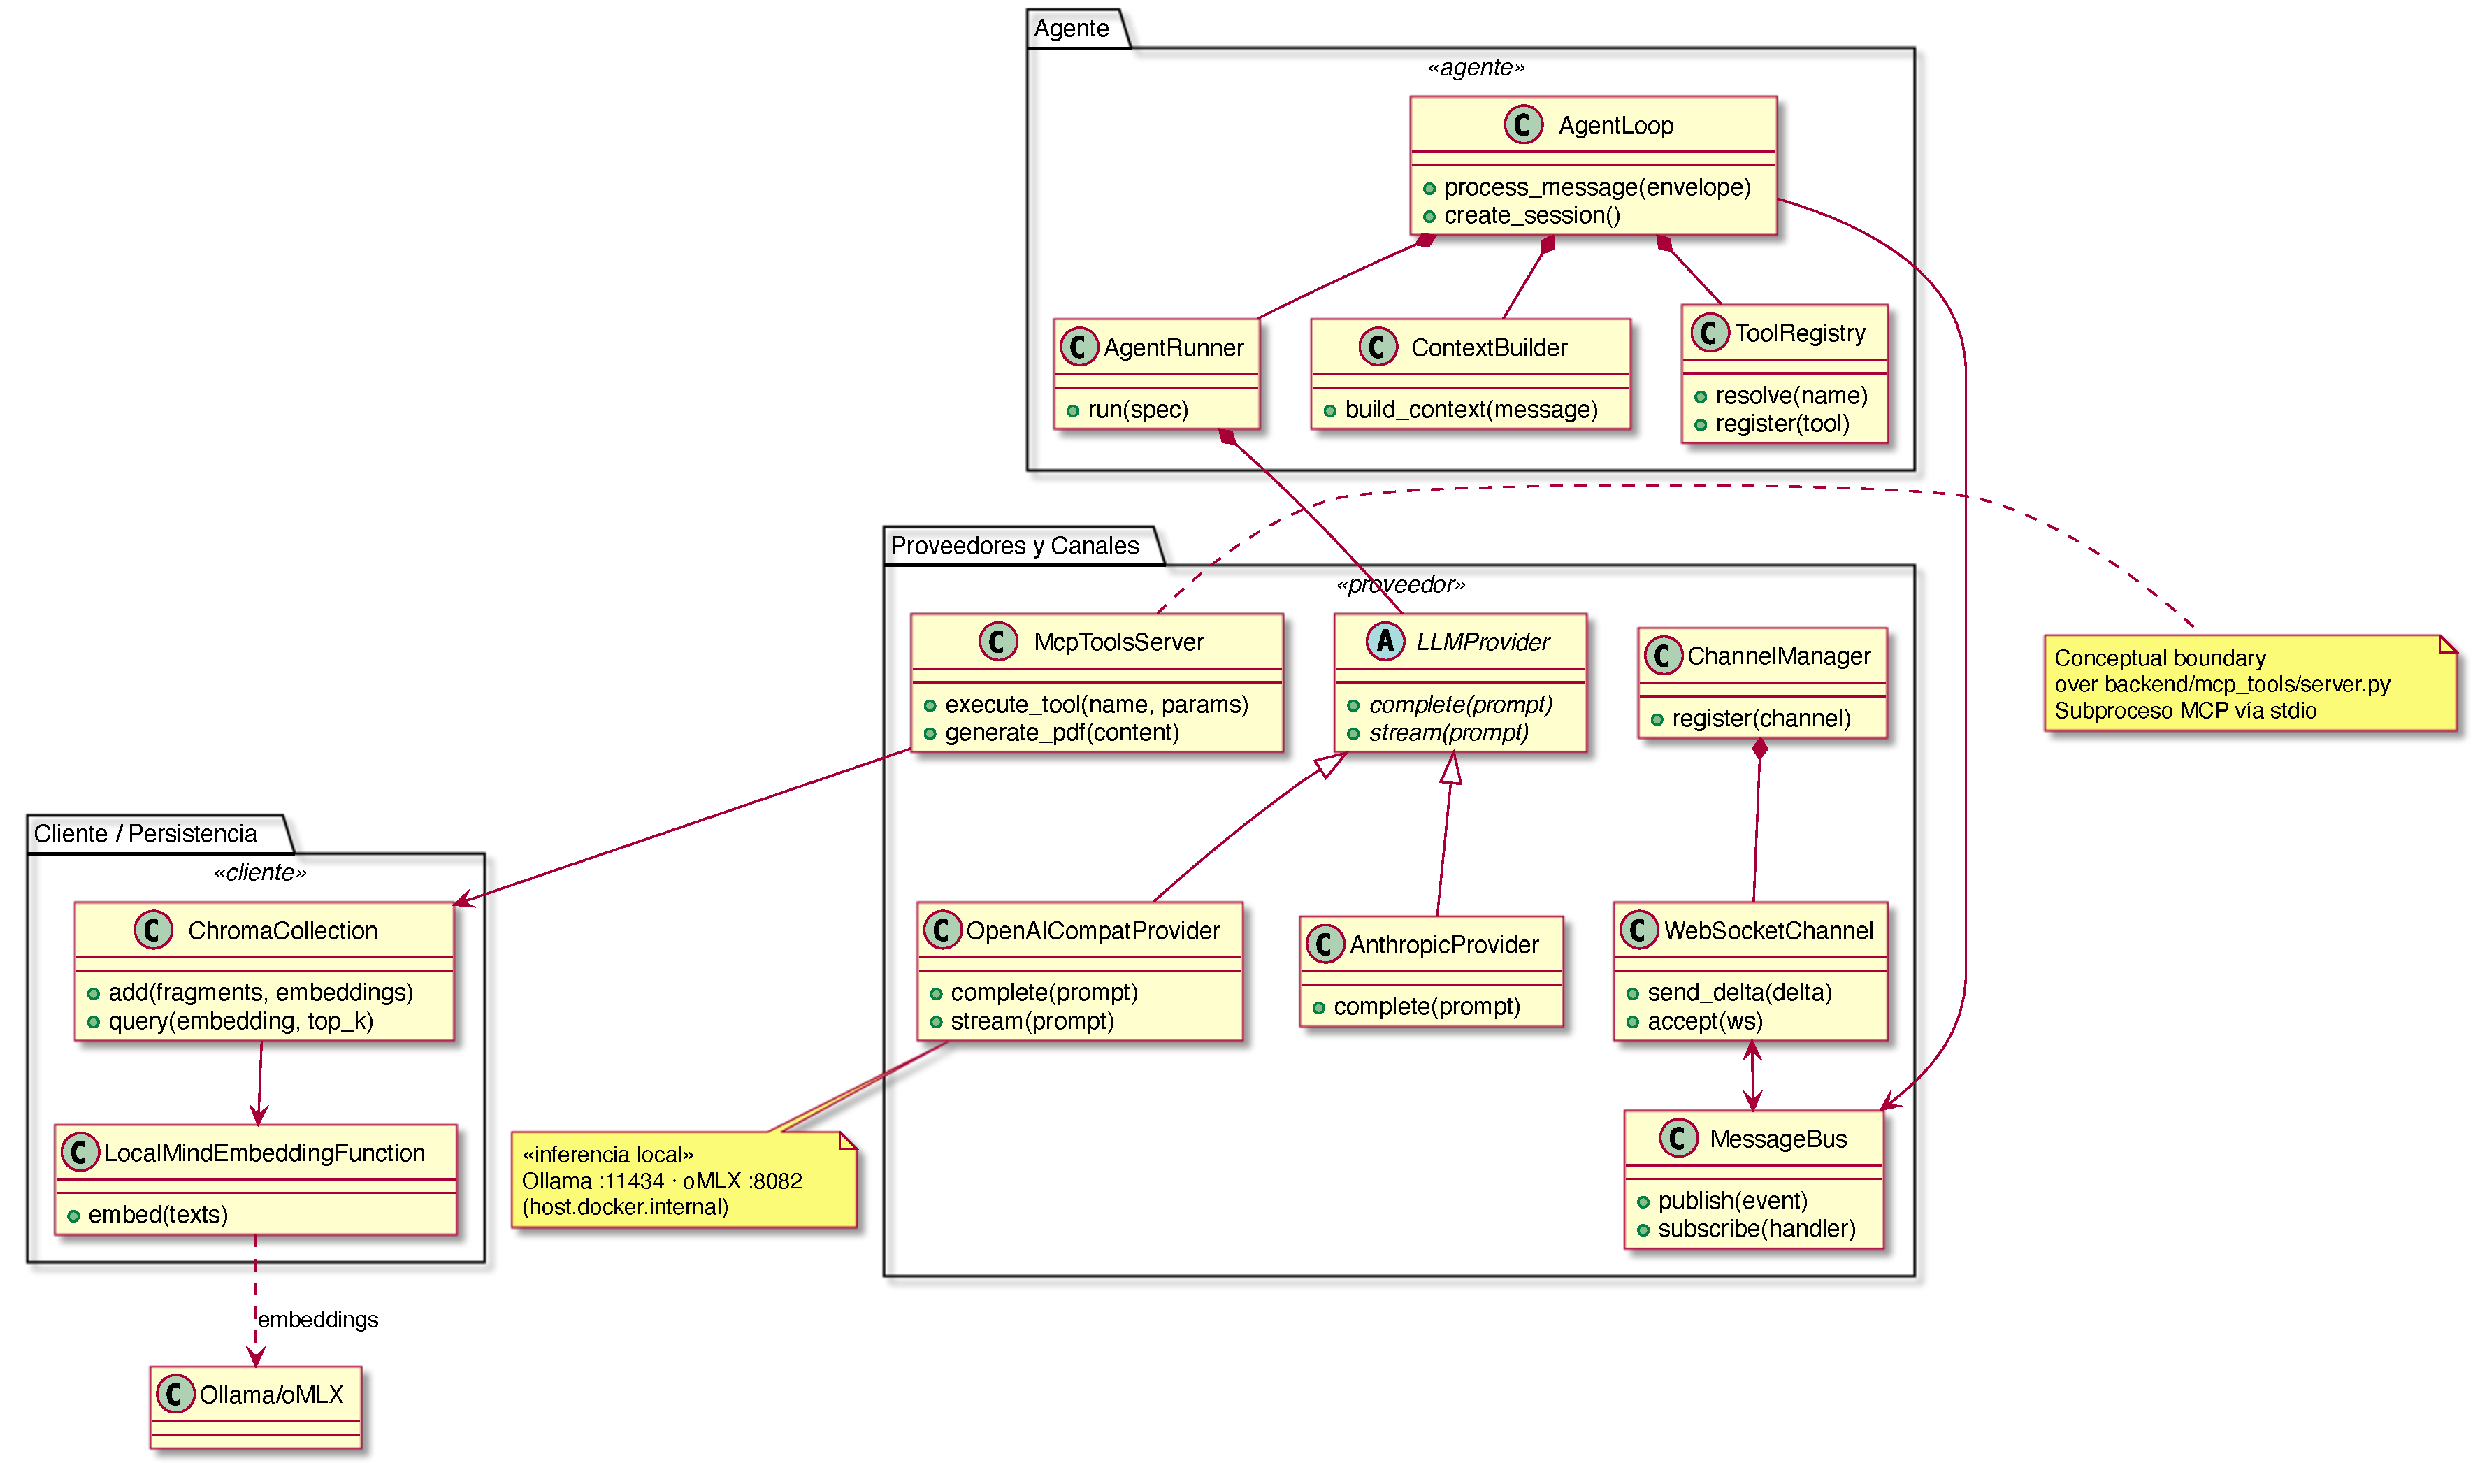
\includegraphics[width=1.0\textwidth]{figs/diagrama-clases-general.pdf}
  \caption{Diagrama de clases general del sistema.}
  \label{fig:diagramaCG}
\end{figure}

El paquete Agente agrupa las clases que implementan la lógica conversacional. La clase \texttt{AgentLoop} actúa como raíz del agregado y compone a \texttt{AgentRunner}, encargada del bucle de razonamiento y la coordinación de llamadas a herramientas, a \texttt{ContextBuilder}, responsable de ensamblar el contexto con el historial, la memoria y la información de la base vectorial, y a \texttt{ToolRegistry}, que mantiene el registro de herramientas \gls{mcp} disponibles. Las relaciones de composición se representan gráficamente mediante líneas con rombo negro relleno, indicando formalmente que el bucle del agente posee y administra el ciclo de vida de estos colaboradores principales.

El paquete Proveedores y Canales contiene las clases que gestionan la inferencia, los canales de comunicación y las herramientas externas. La clase abstracta \texttt{LLMProvider} define los métodos de generación completa y continua, siendo heredada por \texttt{OpenAICompatProvider} y \texttt{AnthropicProvider}. La clase \texttt{OpenAICompatProvider} constituye el adaptador de inferencia local para los motores \gls{ollama} en el puerto 11434 y \gls{omlx} en el puerto 8082. Por su parte, \texttt{ChannelManager} administra el canal activo \texttt{WebSocketChannel} en el puerto 8765. La barra de eventos \texttt{MessageBus} desacopla la recepción de mensajes del procesamiento del agente, mientras que \texttt{McpToolsServer} representa el servidor de herramientas \gls{mcp} que se ejecuta en subproceso con comunicación por entrada y salida estándar.

El paquete Cliente y Persistencia agrupa a \texttt{ChromaCollection}, que abstrae las colecciones de la base vectorial \gls{chromadb} para almacenar y consultar vectores, y a \texttt{LocalMindEmbeddingFunction}, que delega en el motor de inferencia local para generar los vectores correspondientes. La relación de dependencia entre ambas clases indica que la colección de \gls{chromadb} utiliza dicha función para convertir los textos en vectores antes de su almacenamiento o consulta.

\section{Diagramas de actividades más relevantes del análisis}

Esta sección presenta dos diagramas de actividades complementarios que describen los flujos operativos más densos y relevantes del sistema: el protocolo de razonamiento \gls{cotrag} del agente, en la Figura~\ref{fig:diagramaAP1}, y el flujo de comunicación y ciclo de vida del canal \gls{websocket}, en la Figura~\ref{fig:diagramaAP2}.

\subsection{Protocolo CoT-RAG}

La Figura~\ref{fig:diagramaAP1} describe el diagrama de actividades de cinco pasos que el agente sigue para procesar cada mensaje recibido de la persona usuaria.

\begin{figure}[h!tp]
  \centering
  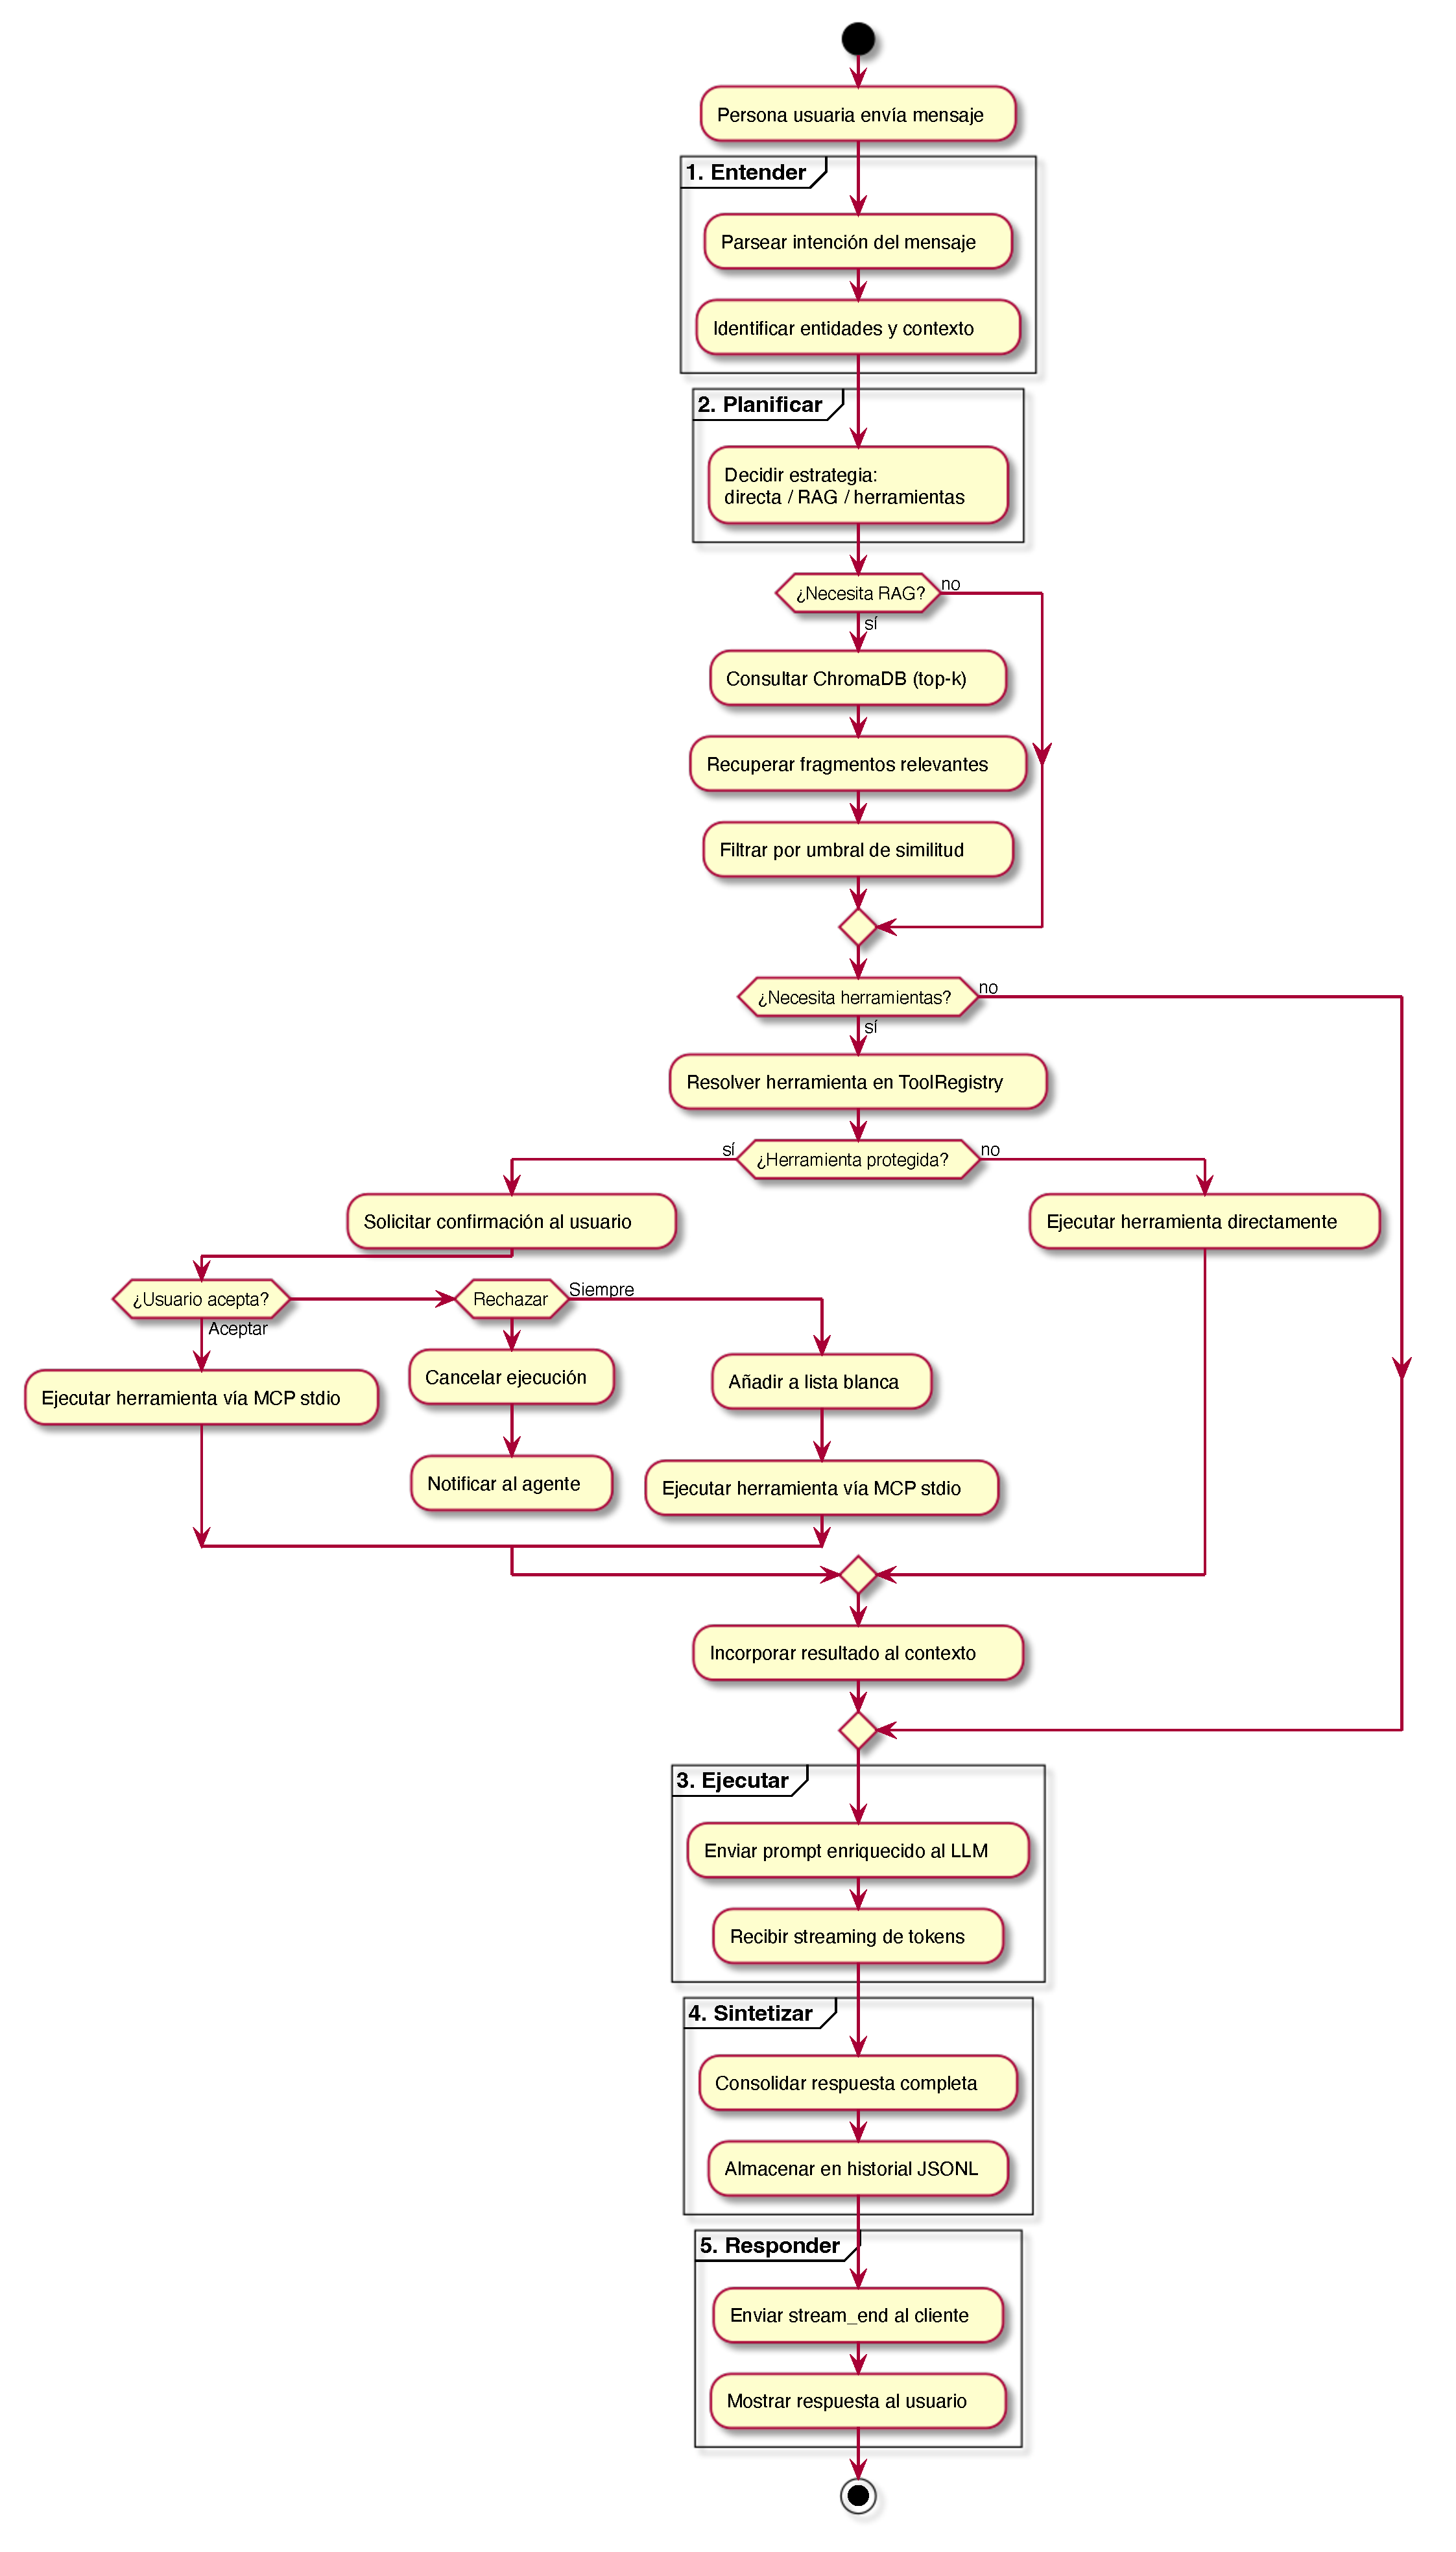
\includegraphics[width=\textwidth, height=0.82\textheight, keepaspectratio]{figs/diagrama-actividades-cot-rag.pdf}
  \caption{Diagrama de actividades del protocolo \gls{cotrag}.}
  \label{fig:diagramaAP1}
\end{figure}

El protocolo se inicia con la fase de comprensión, en la que el agente analiza la intención del mensaje e identifica las entidades y el contexto relevantes. A continuación, la fase de planificación decide la estrategia a seguir mediante respuesta directa, consulta a la base de conocimiento, invocación de herramientas o una combinación de las mismas.

Si el agente determina que requiere información de la base de conocimiento, se ejecuta la fase de búsqueda vectorial consultando \gls{chromadb} con los vectores de la solicitud, recuperando los fragmentos más próximos y filtrándolos por el umbral de similitud semántica establecido en el caso de uso CU5. Si la estrategia contempla invocar herramientas, el agente localiza la herramienta en el registro y la ejecuta mediante el servidor \gls{mcp}. Cuando la herramienta se encuentra clasificada como protegida, se solicita la confirmación explícita de la persona usuaria, quien puede aceptar, rechazar o autorizar la herramienta en lista blanca. En caso de rechazo, la ejecución se cancela y se notifica la interrupción al agente.

Tras la fase de ejecución, el agente pasa a la fase de síntesis, en la cual consolida la respuesta completa, integra los resultados de las herramientas y el contexto recuperado, y guarda la respuesta en el archivo de sesión. Finalmente, la fase de respuesta envía el evento de cierre al cliente y muestra el resultado en la interfaz.

\subsection{Ciclo de vida y comunicación del WebSocket}

La Figura~\ref{fig:diagramaAP2} detalla el diagrama de actividades que rige el establecimiento de la conexión \gls{websocket}, la recepción de eventos, la emisión en emisión continua y la gestión de reconexiones automáticas ante fallos de red.

\begin{figure}[h!tp]
  \centering
  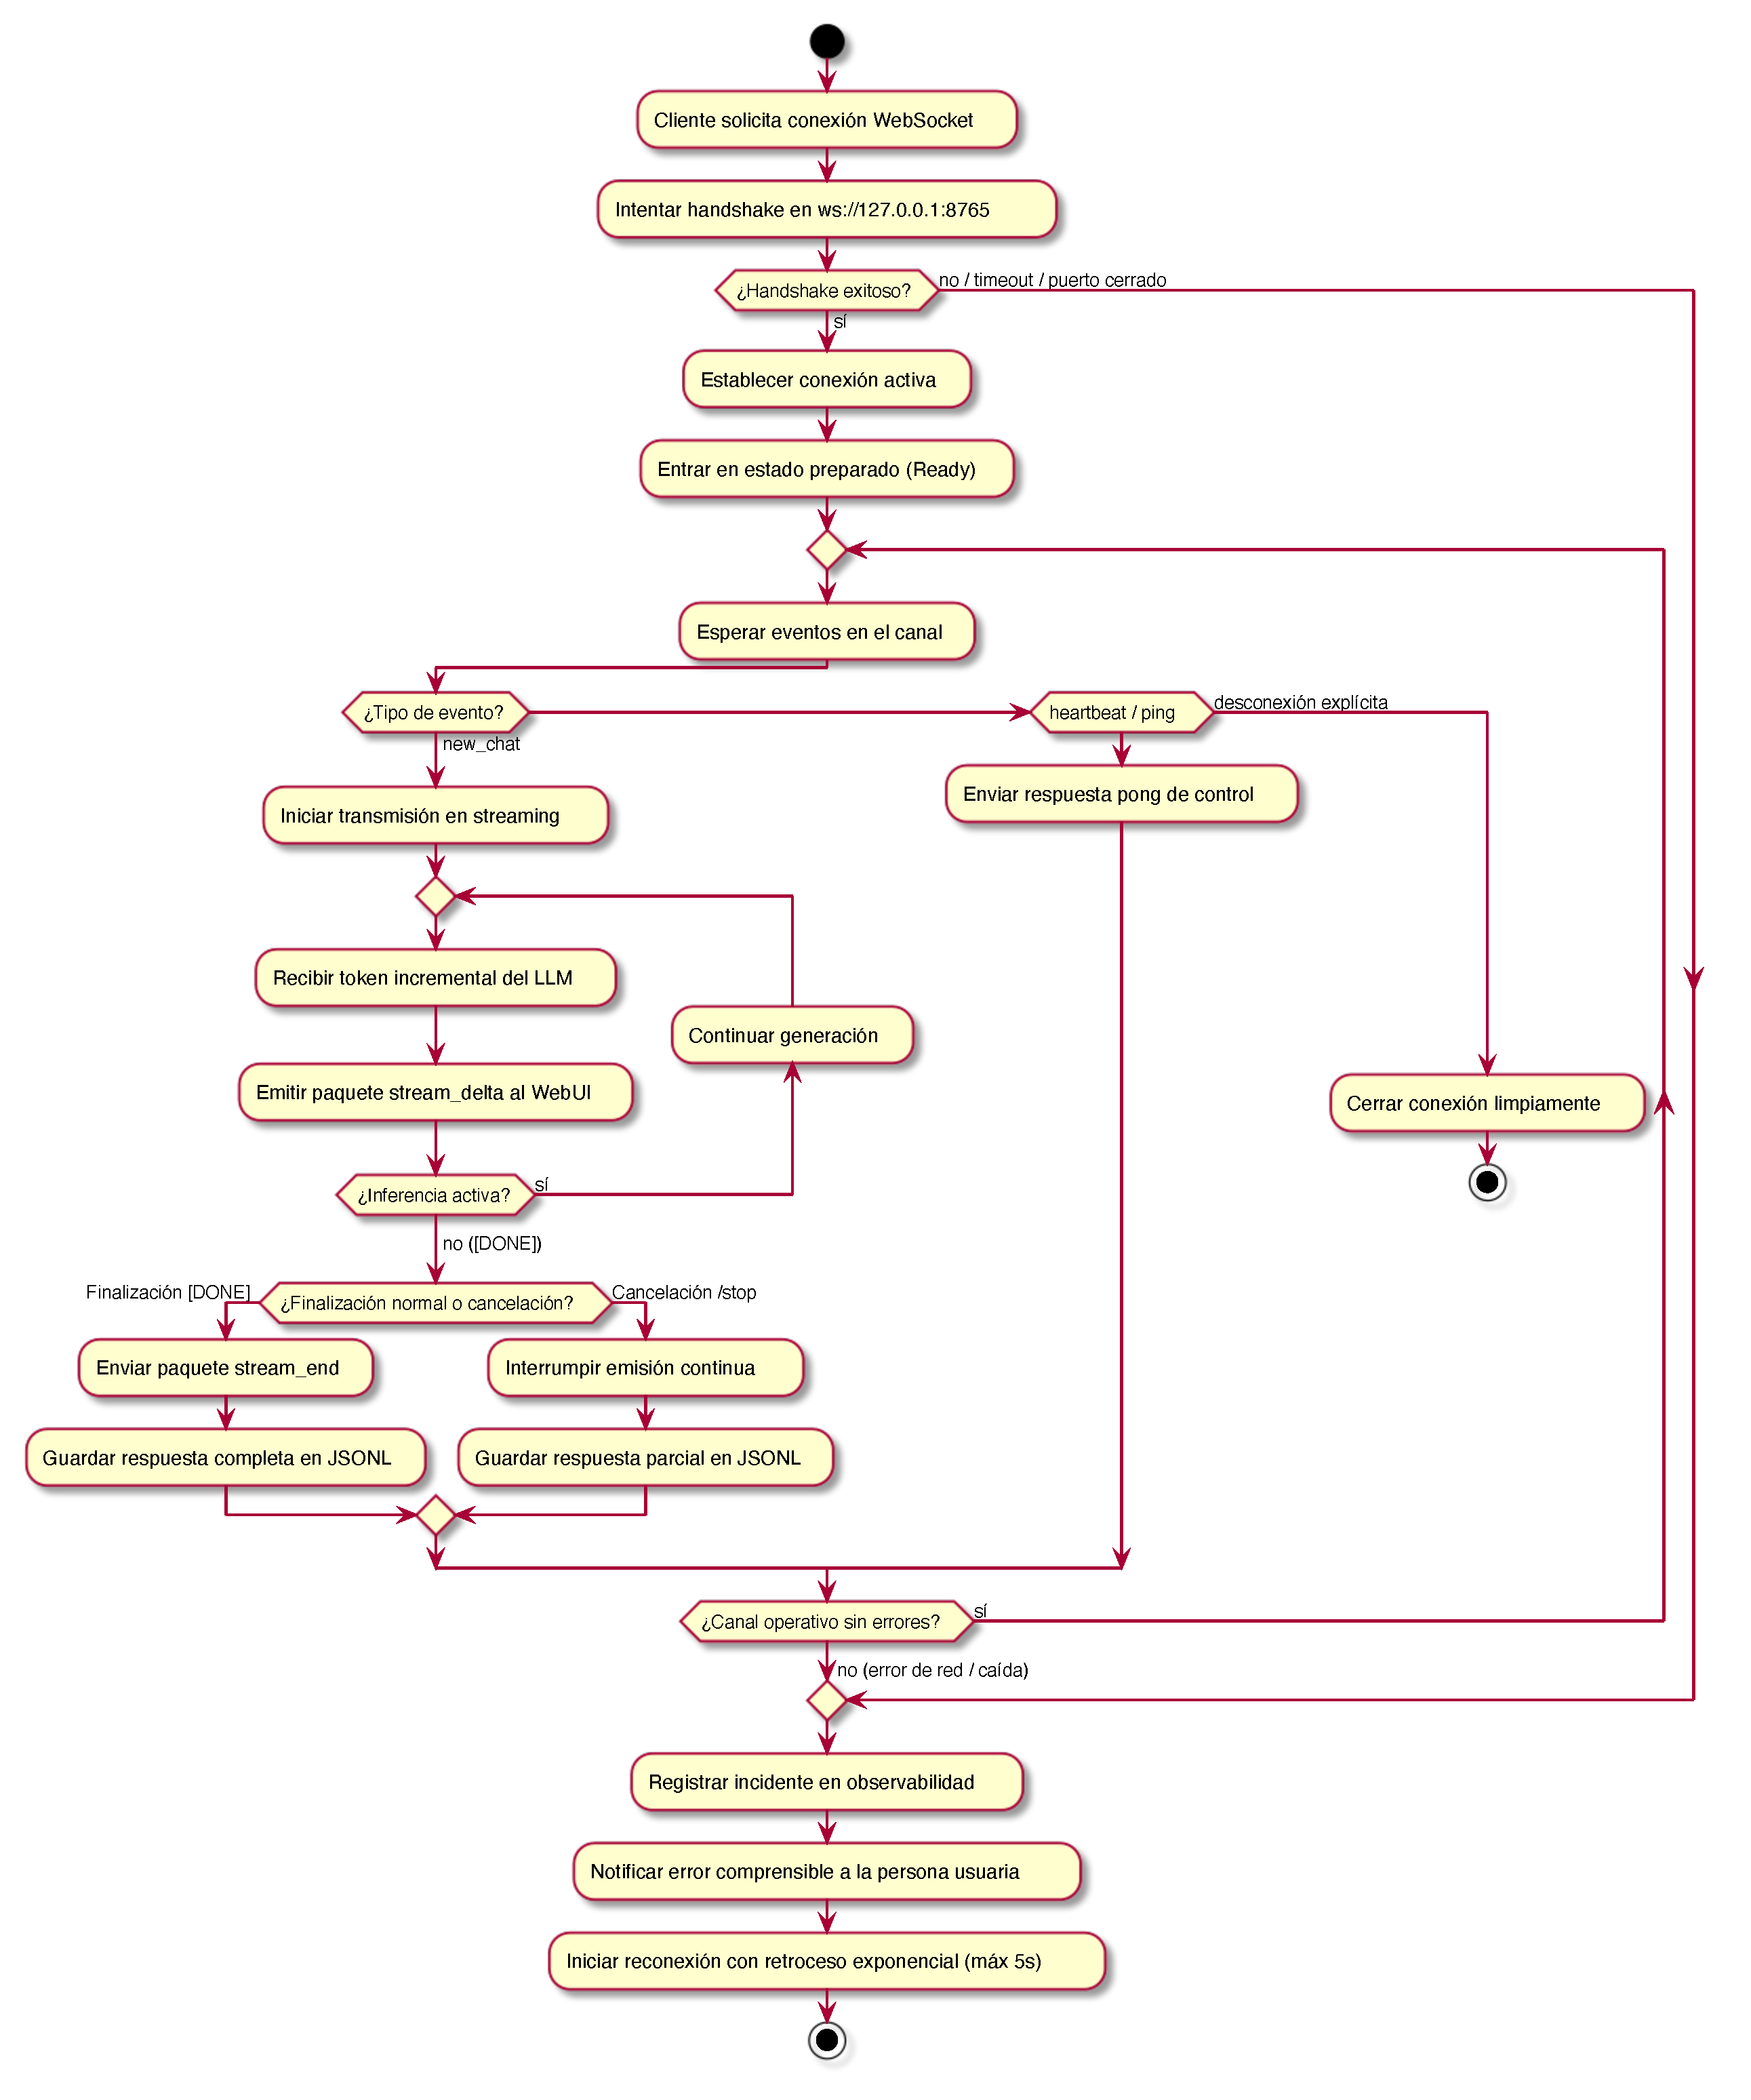
\includegraphics[width=\textwidth, height=0.82\textheight, keepaspectratio]{figs/diagrama-actividades-websocket.pdf}
  \caption{Diagrama de actividades del canal de comunicación \gls{websocket}.}
  \label{fig:diagramaAP2}
\end{figure}

El flujo se inicia cuando el cliente solicita la conexión e intenta el saludo inicial en la dirección \texttt{ws://127.0.0.1:8765}. Si la negociación resulta exitosa, la conexión entra en el estado preparado a la espera de peticiones o de señales de control periódicas.

Al recibir un evento de tipo \texttt{new\_chat}, el canal inicia la transmisión en emisión continua emitiendo paquetes incrementales hacia la interfaz web a medida que el motor genera cada token. Si la inferencia concluye normalmente, se transmite el evento de cierre y se registra la respuesta completa en el historial \gls{jsonl}; si se recibe una orden de interrupción \texttt{/stop}, la emisión se cancela inmediatamente guardando la respuesta parcial. Si se produce una caída de red o un tiempo de espera agotado, el flujo notifica el incidente a la persona usuaria y activa el proceso de reconexión con retroceso exponencial hasta un máximo de cinco segundos.

\section*{Resumen y enlaces entre capítulos}

Este capítulo ha presentado el análisis del sistema LocalMind-AI mediante nueve casos de uso que cubren los requisitos funcionales y no funcionales, un diagrama de secuencia que describe el flujo conversacional completo, un diagrama de clases estructurado en tres paquetes principales y dos diagramas de actividades que detallan el protocolo \gls{cotrag} y el canal de comunicación \gls{websocket}. La traducción de estos casos de uso a componentes de software se desarrolla en el Capítulo~\ref{ch:diseno} (Diseño); su implementación y verificación se describe en el Capítulo~\ref{ch:implementacion} (Implementación y Pruebas).

\chapter{Diseño}\label{ch:diseno}
% % Contenidos del capítulo.
% Las secciones presentadas son orientativas y no representan
% necesariamente la organización que debe tener este capítulo.

% Diagramas de clases, de secuencia, de despliegue, diseño de
% pantallas, etc

En esta sección se presenta el diseño arquitectónico del sistema, el cual se representa mediante diagramas de componentes que describen la estructura de cada uno de los subsistemas que conforman la aplicación. A continuación, se incluirán diagramas de secuencia detallados que ilustran, de manera precisa, el comportamiento y la interacción de los distintos componentes dentro de cada subsistema, en función de sus respectivas funcionalidades.

Seguidamente, se incorpora un diagrama de despliegue, en el que se identifican los nodos físicos de ejecución, así como la forma en que los distintos componentes lógicos son empaquetados e implementados en el software correspondiente.

Finalmente, se incluye un wireframe de la interfaz de usuario/a del add-on, con el propósito de mostrar la disposición visual del panel y facilitar la comprensión de su estructura funcional. Con todo ello, se proporciona una visión global y estructurada de la aplicación, tanto desde la perspectiva del diseño como de su futura implementación y despliegue.

\section{Arquitectura general del sistema}
La estructura general del sistema está constituida por dos subsistemas principales, como se ilustra en la Figura~\ref{fig:diagramaAGS}.
Dentro de estos subsistemas se encuentran los componentes que los integran y las relaciones entre ellos.
\begin{figure}[h!tp]
  \centering
  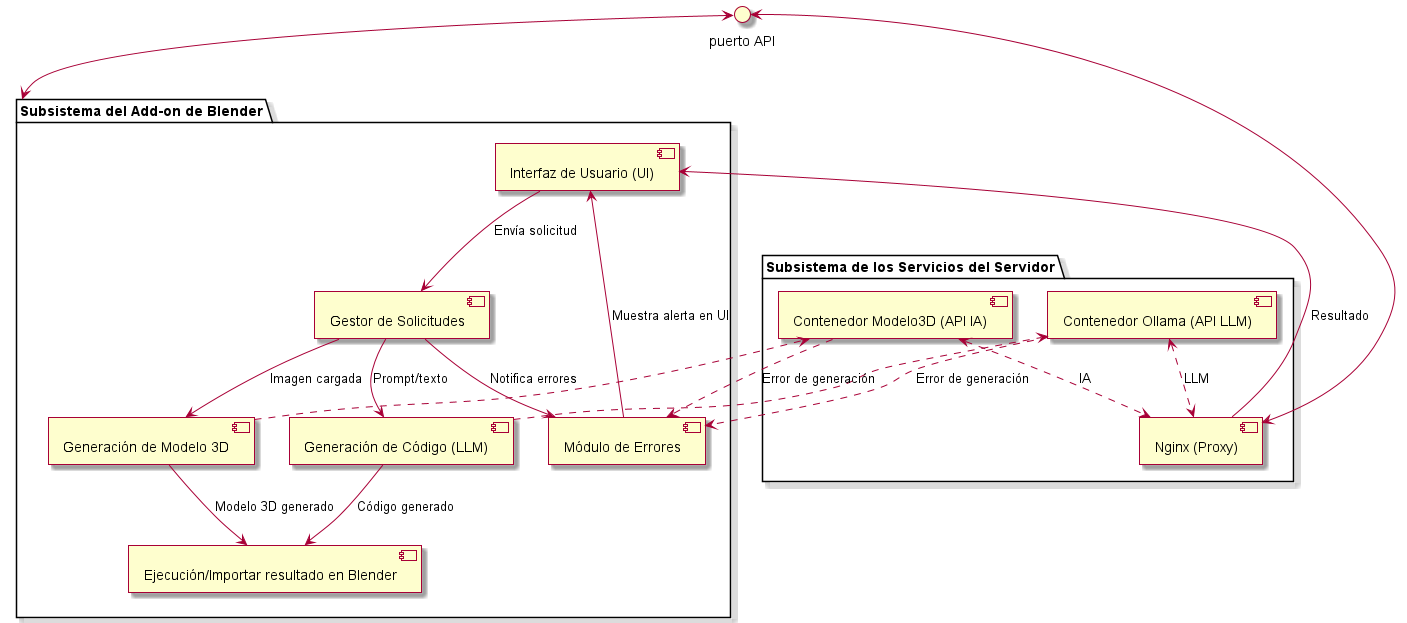
\includegraphics[width=1.1\textwidth]{figs/DiagramaArquitecturaGeneral.png}
  \caption{Diagrama de arquitectura general del sistema.}
  \label{fig:diagramaAGS}
\end{figure}

El primer subsistema consiste en el add-on de Blender, el cual proporciona la interfaz gráfica que el usuario/a emplea para interactuar al cargar imágenes, exportar los resultados de la generación 3D o utilizar modelos de inteligencia artificial. Este subsistema también gestiona las solicitudes tanto al modelo de lenguaje \gls{llm} como al modelo de generación de elementos 3D, procesa las respuestas de las \glspl{ia} generando el código Python en el caso del modelo \gls{llm} o generando el modelo 3D con el modelo generativo 3D y ejecuta dicho código Python o posiciona el modelo 3D en el entorno de Blender. Todo esto se realiza de manera no bloqueante para la aplicación, manejando cualquier posible error que ocurra e informando de ello.

El segundo subsistema está constituido por el servicio dockerizado, el cual alberga la API sobre Nginx que actúa como el componente orquestador principal y proxy, redirigiendo todas las solicitudes al modelo de \gls{ia} pertinente. En consecuencia, los demás componentes comprenden el contenedor del modelo de \gls{llm} y el contenedor del modelo generativo 3D, los cuales procesan las solicitudes recibidas y generan una respuesta o informan de un error.

% Imagen diagrama de arquitectura general del sistema


\section{Arquitectura de componentes}
% A partir de la especificación realizada en la sección \ref{sec:especificaciones-sistema} del Capítulo \ref{ch:requisitos} y la tecnología seleccionada en la sección \ref{sec:evaluacion-tecnologias} del Capítulo \ref{ch:estado-arte}, se debe construir el diagrama de componentes UML que represente la arquitectura de referencia del sistema. 
% En este diagrama se deben identificar los componentes principales del sistema y las relaciones entre ellos, pasando a detallar los subcomponentes de cada uno de ellos en secciones posteriores.
A continuación, se presentan los diagramas de componentes correspondientes a cada uno de los subsistemas del sistema propuesto, junto con sus respectivos diagramas de secuencia, los cuales describen en detalle las funciones específicas que ejecuta cada conjunto de componentes. Además, se indica el entorno tecnológico y el software utilizado en la implementación de dichas funcionalidades, permitiendo una visión clara de la distribución estructural y del flujo operativo dentro de la arquitectura del sistema. Es importante señalar que el elemento relacionado con la interfaz de usuario no se ha abordado en esta sección, porque en el apartado titulado "Wireframe de la pantalla del Add-on", se describe detalladamente esa interfaz junto con el correspondiente wireframe de la misma.

\subsection{Subsistema del add-on de Blender}
Este subsistema corresponde al complemento (add-on) desarrollado para su integración en el entorno Blender, permitiendo su instalación en múltiples dispositivos siempre que se utilice la versión 3.6 del software. En esta sección se analiza la estructura interna del complemento, describiendo el flujo completo de procesamiento, que abarca desde la entrada de una imagen o instrucción por parte del usuario hasta la recepción, ejecución, importación y exportación de resultados generados por los modelos de inteligencia artificial en el entorno de Blender. Este subsistema ha sido íntegramente desarrollado utilizando el lenguaje Python, dado que este es el lenguaje requerido para la elaboración de complementos en Blender.

La Figura~\ref{fig:diagramaGS1} presenta el diagrama de componentes del gestor de solicitudes del add-on. Este módulo actúa como núcleo de enrutamiento en el add-on, determinando si la petición debe ser redirigida al LLM o al modelo generativo 3D, gestionando dicha decisión mediante la invocación de la función Fetch correspondiente. Además, en caso de producirse errores durante el proceso, estos se comunican al módulo de notificación, que a su vez informa al usuario.
% Imagen diagrama componente 1
\begin{figure}[h!tp]
  \centering
  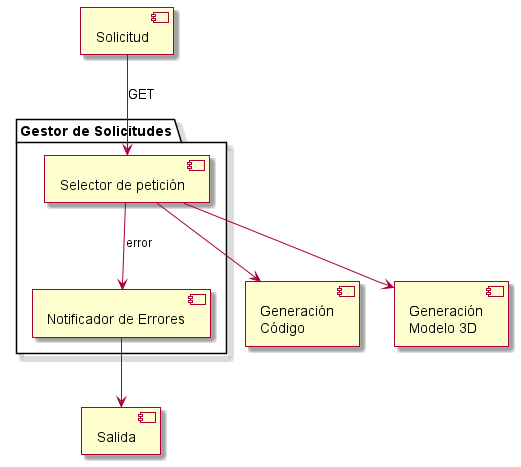
\includegraphics[width=0.8\textwidth]{figs/DiagramaComponentesGS.png}
  \caption{Diagrama de componentes del gestor de solicitudes del add-on.}
  \label{fig:diagramaGS1}
\end{figure}
El diagrama de secuencia asociado, mostrado en la Figura~\ref{fig:diagramaGS2}, detalla de manera precisa el comportamiento dinámico de este flujo.

% Imagen diagrama secuencia 1
\begin{figure}[h!tp]
  \centering
  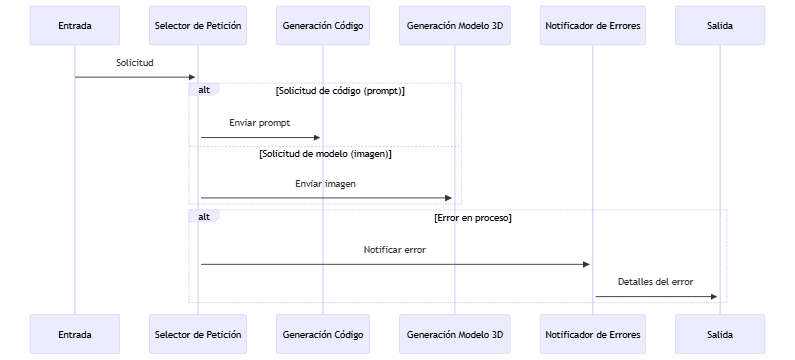
\includegraphics[width=1.1\textwidth]{figs/DiagramaSecuenciaGS.png}
  \caption{Diagrama de secuencia del gestor de solicitudes del add-on.}
  \label{fig:diagramaGS2}
\end{figure}



Por otro lado, la Figura~\ref{fig:diagramaGLLM1} presenta el diagrama de componentes correspondiente al módulo de generación de código Python, cuya función principal es gestionar el envío del prompt textual introducido por el usuario hacia el contenedor de Docker que aloja el modelo \gls{llm} de Ollama, a través de la API REST que integra el modelo de Ollama. La respuesta generada por el modelo es procesada mediante un filtro lógico, encargado de extraer exclusivamente el bloque de código Python relevante. Una vez depurado, el resultado se redirige al módulo de salida para su visualización o ejecución. En caso de que se produzcan errores durante la solicitud (fetch) o en el filtrado de la respuesta, estos son canalizados hacia el módulo de gestión de errores, el cual emite una notificación informativa hacia la salida correspondiente.
El comportamiento detallado de este proceso se encuentra descrito en el diagrama de secuencia de la Figura~\ref{fig:diagramaGLLM2}.
% Imagen diagrama componente 2
\begin{figure}[h!tp]
  \centering
  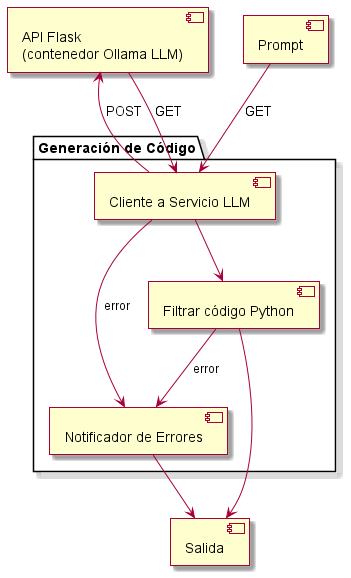
\includegraphics[width=0.5\textwidth]{figs/DiagramaComponentesGC.png}
  \caption{Diagrama de componentes de la generación de código.}
  \label{fig:diagramaGLLM1}
\end{figure}

% Imagen diagrama secuencia 2
\begin{figure}[h!tp]
  \centering
  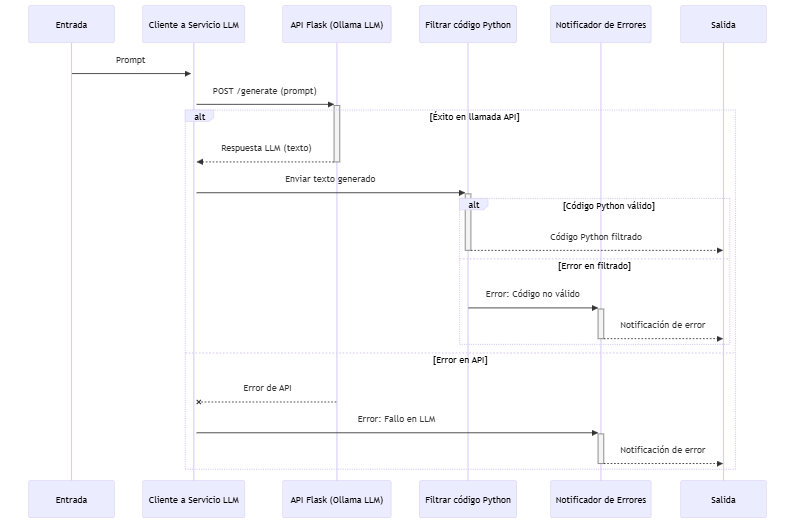
\includegraphics[width=1.1\textwidth]{figs/DiagramaSecuenciaGC.png}
  \caption{Diagrama de secuencia de la generación de código.}
  \label{fig:diagramaGLLM2}
\end{figure}

La Figura~\ref{fig:diagramaGM3D1} representa el diagrama de componentes correspondiente al proceso de generación de modelos tridimensionales a partir de imágenes. Este módulo es responsable de recibir una imagen proporcionada por el usuario y transmitirla, mediante una solicitud fetch, al contenedor Docker donde se ejecuta el modelo de inteligencia artificial 3D, accesible a través de la API Flask propia del modelo. Una vez procesada la imagen, el sistema retorna un modelo 3D generado, que es dirigido directamente al módulo de salida para su posterior utilización. En caso de producirse errores durante el envío de la solicitud o en la gestión de la respuesta, dichos errores son derivados al gestor de notificaciones, encargado de informar al usuario mediante la salida correspondiente.
% Imagen diagrama componente 3
\begin{figure}[h!tp]
  \centering
  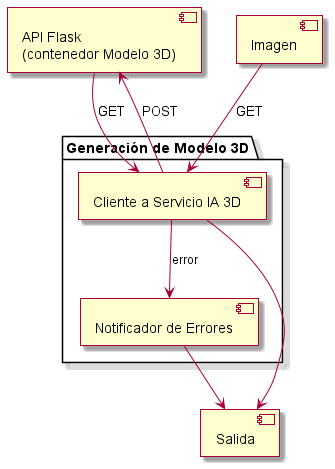
\includegraphics[width=0.5\textwidth]{figs/DiagramaComponentesGM3D.png}
  \caption{Diagrama de componentes de la generación del modelo 3D.}
  \label{fig:diagramaGM3D1}
\end{figure}
El flujo detallado de esta operación se encuentra descrito en el diagrama de secuencia de la Figura~\ref{fig:diagramaGM3D2}.
% Imagen diagrama secuencia 3
\begin{figure}[h!tp]
  \centering
  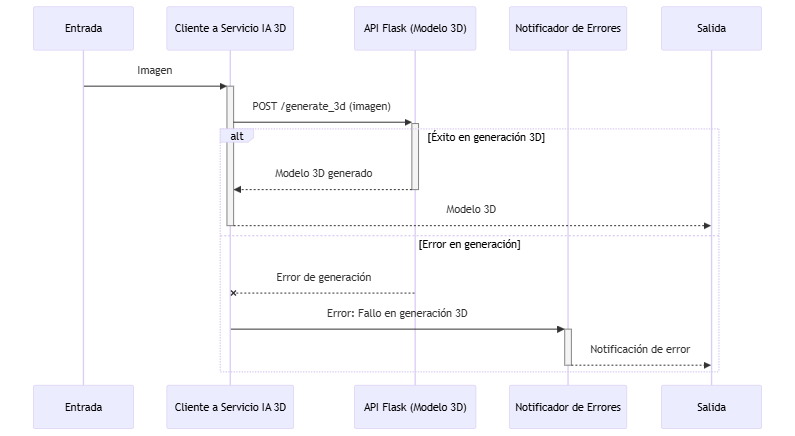
\includegraphics[width=1.1\textwidth]{figs/DiagramaSecuenciaGM3D.png}
  \caption{Diagrama de secuencia de la generación del modelo 3D.}
  \label{fig:diagramaGM3D2}
\end{figure}

La Figura~\ref{fig:diagramaEIB1} presenta el diagrama de componentes del módulo responsable de las operaciones de ejecución, importación y exportación dentro del entorno de Blender.
% Imagen diagrama componente 4
\begin{figure}[h!tp]
  \centering
  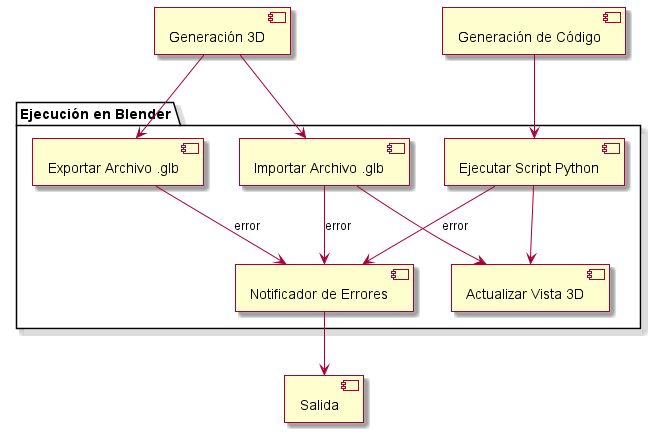
\includegraphics[width=0.8\textwidth]{figs/DiagramaComponentesEIB.png}
  \caption{Diagrama de componentes de la ejecución/importación/exportación en Blender.}
  \label{fig:diagramaEIB1}
\end{figure}
Este componente actúa en función del tipo de entrada recibida, si se trata de código Python, el sistema procede a ejecutarlo directamente sobre la escena activa, actualizando posteriormente la vista 3D para reflejar los cambios. En caso de recibir un modelo 3D generado, el sistema lo importa automáticamente en la escena, habilitando además su exportación en formato .glb, y actualiza de igual manera la visualización en tiempo real. Ante cualquier fallo detectado durante la ejecución del script, la importación del modelo o el proceso de exportación, el error es redirigido al gestor de errores, que se encarga de emitir una notificación al usuario a través del canal de salida.
El comportamiento detallado de este subsistema puede consultarse en el diagrama de secuencia de la Figura~\ref{fig:diagramaEIB2}.
% Imagen diagrama secuencia 4
\begin{figure}[h!tp]
  \centering
  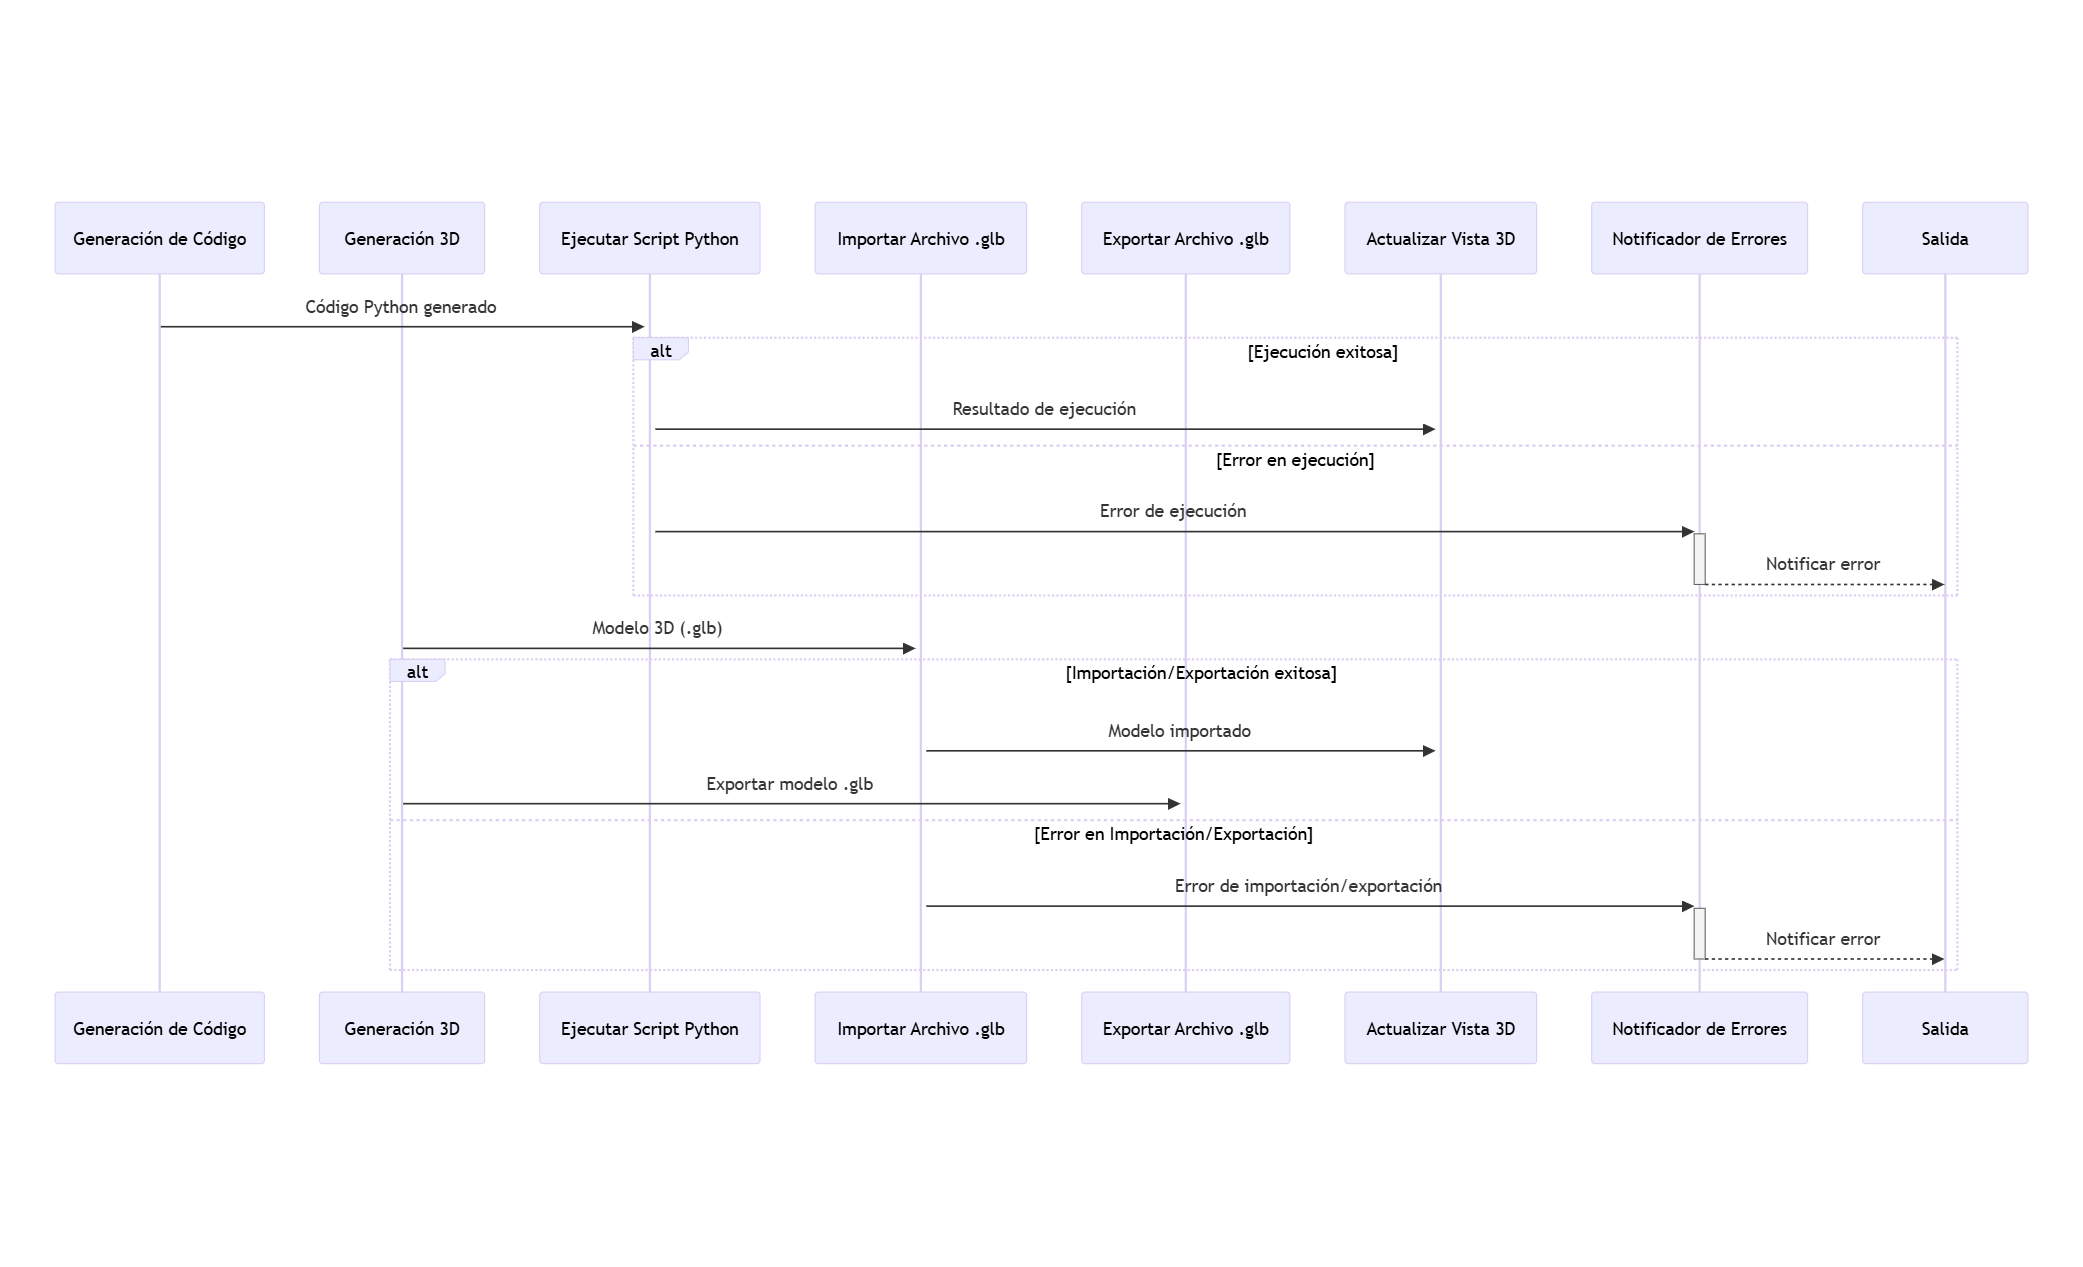
\includegraphics[width=1.1\textwidth]{figs/DiagramaSecuenciaEIB.png}
  \caption{Diagrama de secuencia de la ejecución/importación/exportación en Blender.}
  \label{fig:diagramaEIB2}
\end{figure}



Finalmente, como elemento final del subsistema del add-on de Blender, se presenta la Figura~\ref{fig:diagramaME1}, que ilustra el diagrama de componentes del módulo de gestión de errores. Este módulo tiene como principal función la captura, el procesamiento y el formateo de cualquier tipo de error procedente de otros subsistemas y del mismo. Una vez formateado, el mensaje de error es transmitido al componente de interfaz de usuario mediante la salida adecuada, lo que permite su visualización de manera clara para el usuario. El comportamiento de este módulo, así como su interacción con el resto del sistema, están detallados en el diagrama de secuencia de la Figura~\ref{fig:diagramaME2}.
% Imagen diagrama componente 5
\begin{figure}[h!tp]
  \centering
  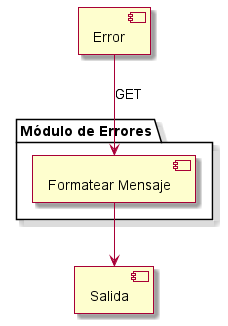
\includegraphics[width=0.4\textwidth]{figs/DiagramaComponentesME.png}
  \caption{Diagrama de componentes del módulo de errores.}
  \label{fig:diagramaME1}
\end{figure}

% Imagen diagrama secuencia 5
\begin{figure}[h!tp]
  \centering
  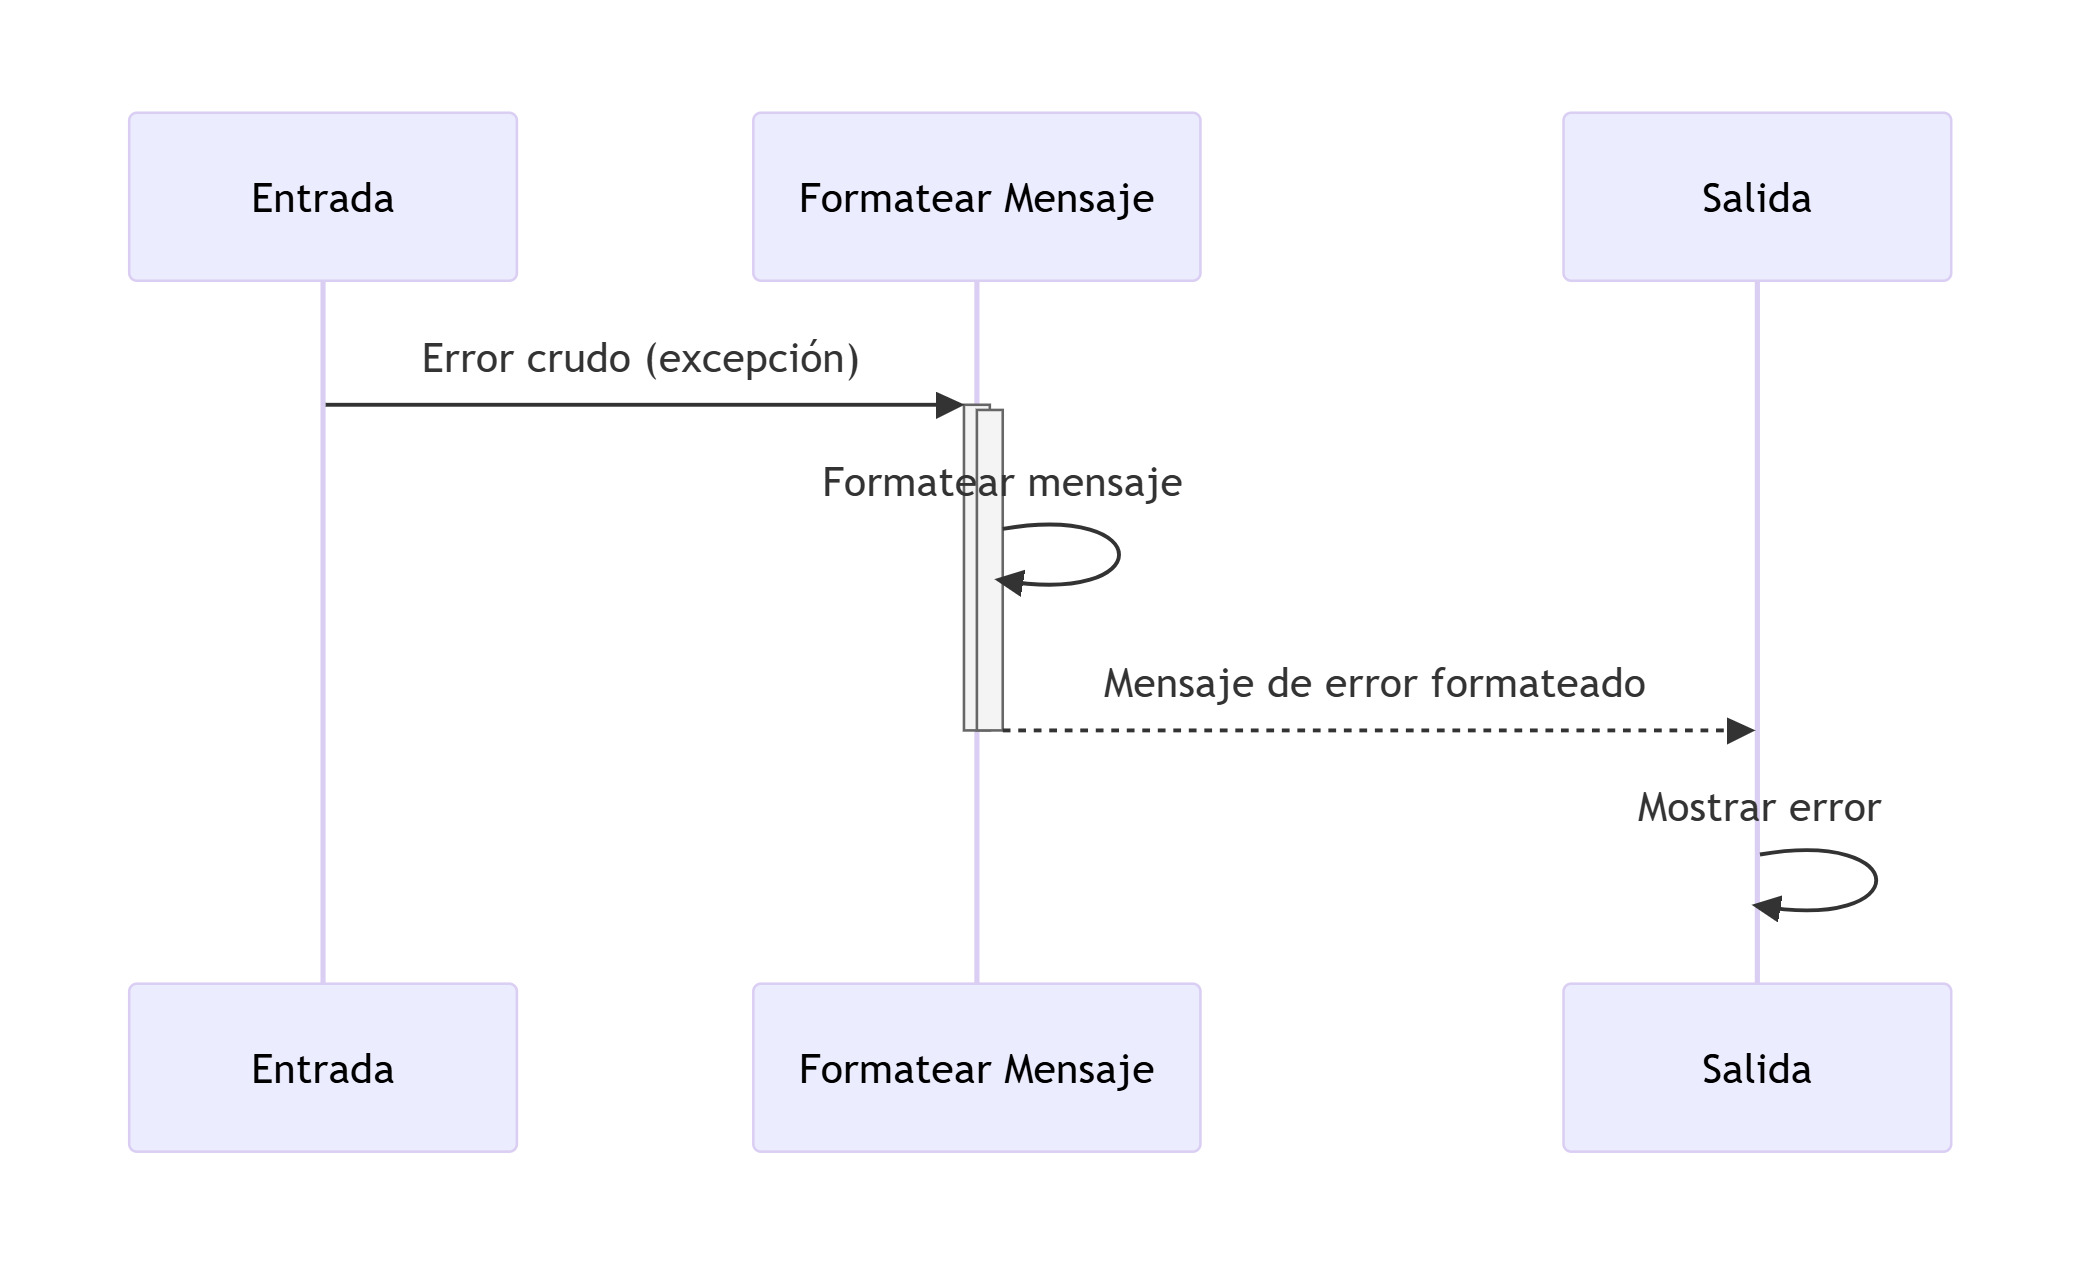
\includegraphics[width=0.8\textwidth]{figs/DiagramaSecuenciaME.png}
  \caption{Diagrama de secuencia del módulo de errores.}
  \label{fig:diagramaME2}
\end{figure}


\subsection{Subsistema de los servicios del servidor}
El segundo y último subsistema corresponde a la infraestructura de servicios dockerizados, diseñada para hacer de proxy y orquestar dinámicamente las solicitudes dirigidas a los modelos de inteligencia artificial, tanto al modelo de lenguaje \gls{llm} como al modelo generativo 3D, a través de una API REST desarrollada con Nginx. Este enfoque de implementación ofrece una arquitectura flexible y escalable, idónea para su posible integración en entornos de producción o sistemas empresariales, al permitir la ejecución concurrente de múltiples peticiones sin bloquear el flujo de procesamiento, gracias a la naturaleza asincrónica del sistema. En esta sección se detalla la estructura interna del servidor de \gls{ia}, describiendo el flujo de procesamiento desde la recepción de entradas en formato texto o imagen a través de la API/proxy, hasta su encaminamiento hacia el contenedor correspondiente que aloja el modelo adecuado. Una vez procesadas, las respuestas generadas por los modelos son gestionadas y devueltas al complemento de Blender, garantizando una integración eficiente entre cliente y servidor. Este subsistema ha sido implementado utilizando el proxy mediante el archivo de configuración de Nginx, mientras que la definición de contenedores y su configuración se ha realizado mediante los lenguajes Dockerfile DSL y YAML para los archivos de Docker Compose del despliegue local.

La Figura~\ref{fig:diagramaAPI1} muestra el diagrama de componentes correspondiente al módulo de la API que hace de proxy mediante Nginx, que actúa como punto central de enrutamiento y coordinación dentro del servidor de inteligencia artificial.

% Imagen diagrama componente 6
\begin{figure}[h!tp]
  \centering
  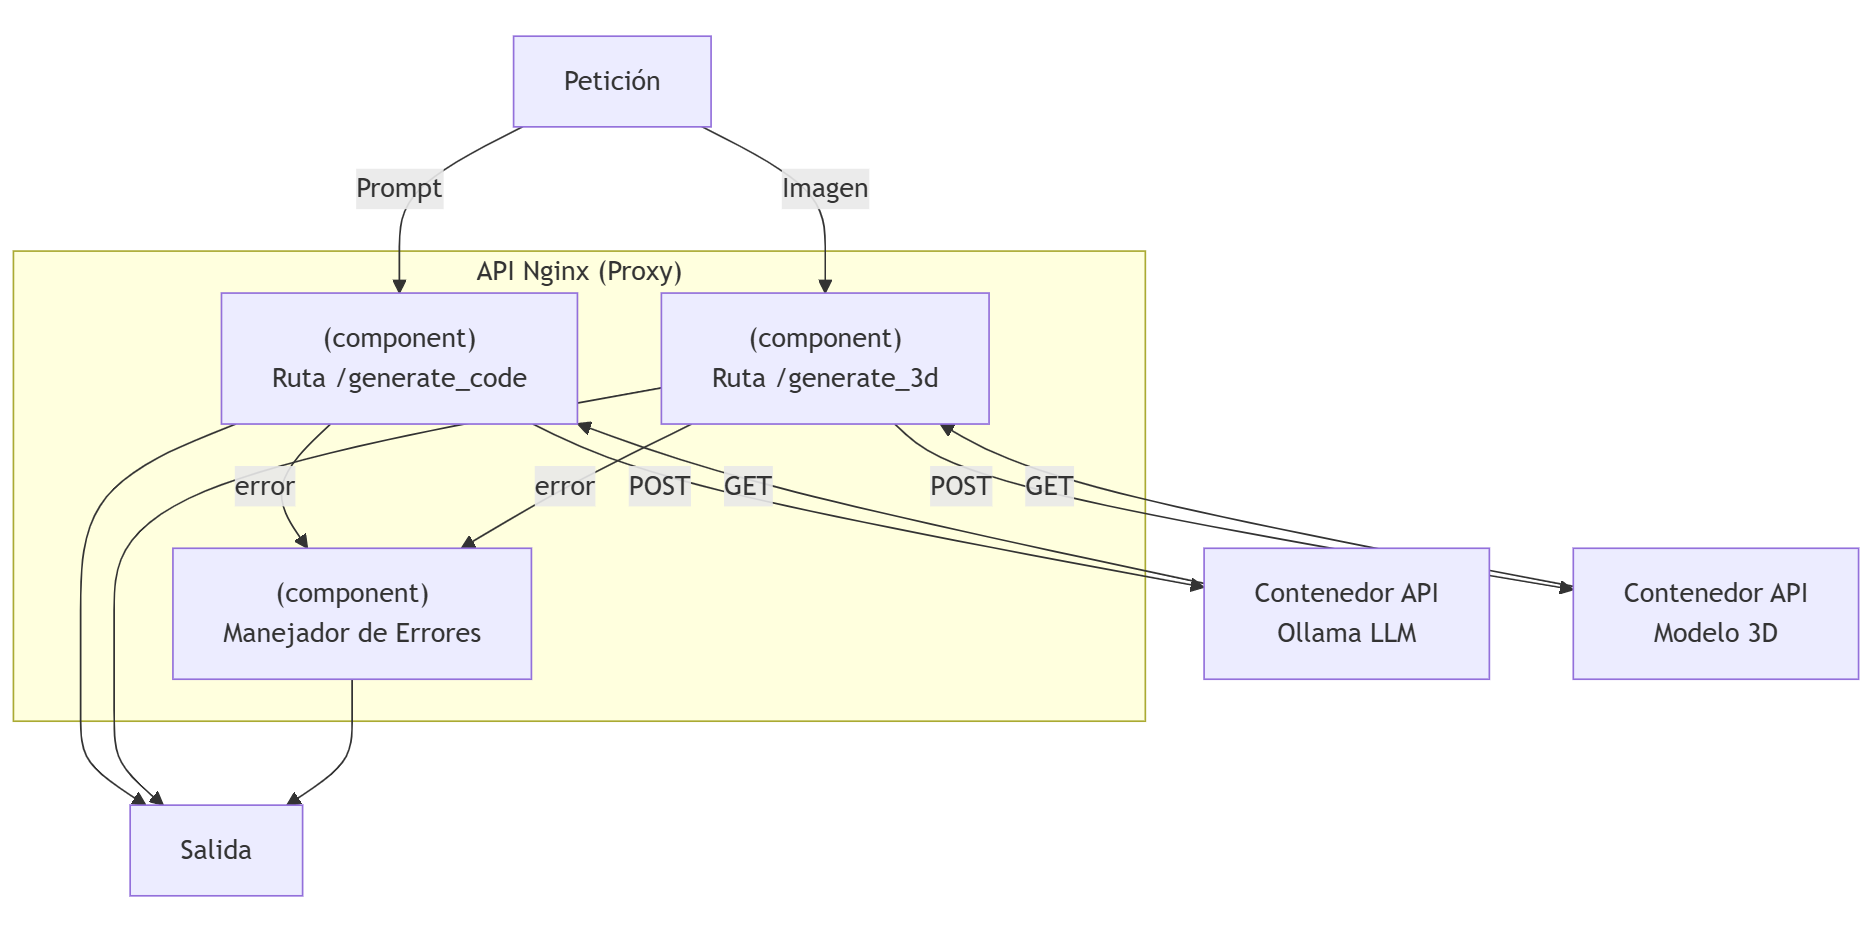
\includegraphics[width=1.1\textwidth]{figs/DiagramaComponentesAPI.png}
  \caption{Diagrama de componentes de la API Nginx.}
  \label{fig:diagramaAPI1}
\end{figure}

Este componente es responsable de analizar cada solicitud entrante proveniente del add-on, identificando si se trata de un prompt textual o de una imagen, y en función de ello, redirigirla al contenedor apropiado, el que aloja el modelo LLM de Ollama o el correspondiente al modelo generativo 3D. La API se encarga de invocar el contenedor seleccionado, gestionar la ejecución del modelo y recoger la respuesta generada, la cual es posteriormente enviada de vuelta al add-on a través del canal de salida del componente. En caso de que se produzcan errores durante el procesamiento, ya sea en la fase de redirección, ejecución o respuesta, estos son transmitidos al módulo de notificación, que se encarga de retornar un mensaje de error informativo al add-on. El diagrama de secuencia presentado en la Figura~\ref{fig:diagramaAPI2} ilustra de manera exhaustiva el flujo de operaciones y decisiones que configuran este comportamiento.


% Imagen diagrama secuencia 6
\begin{figure}[h!tp]
  \centering
  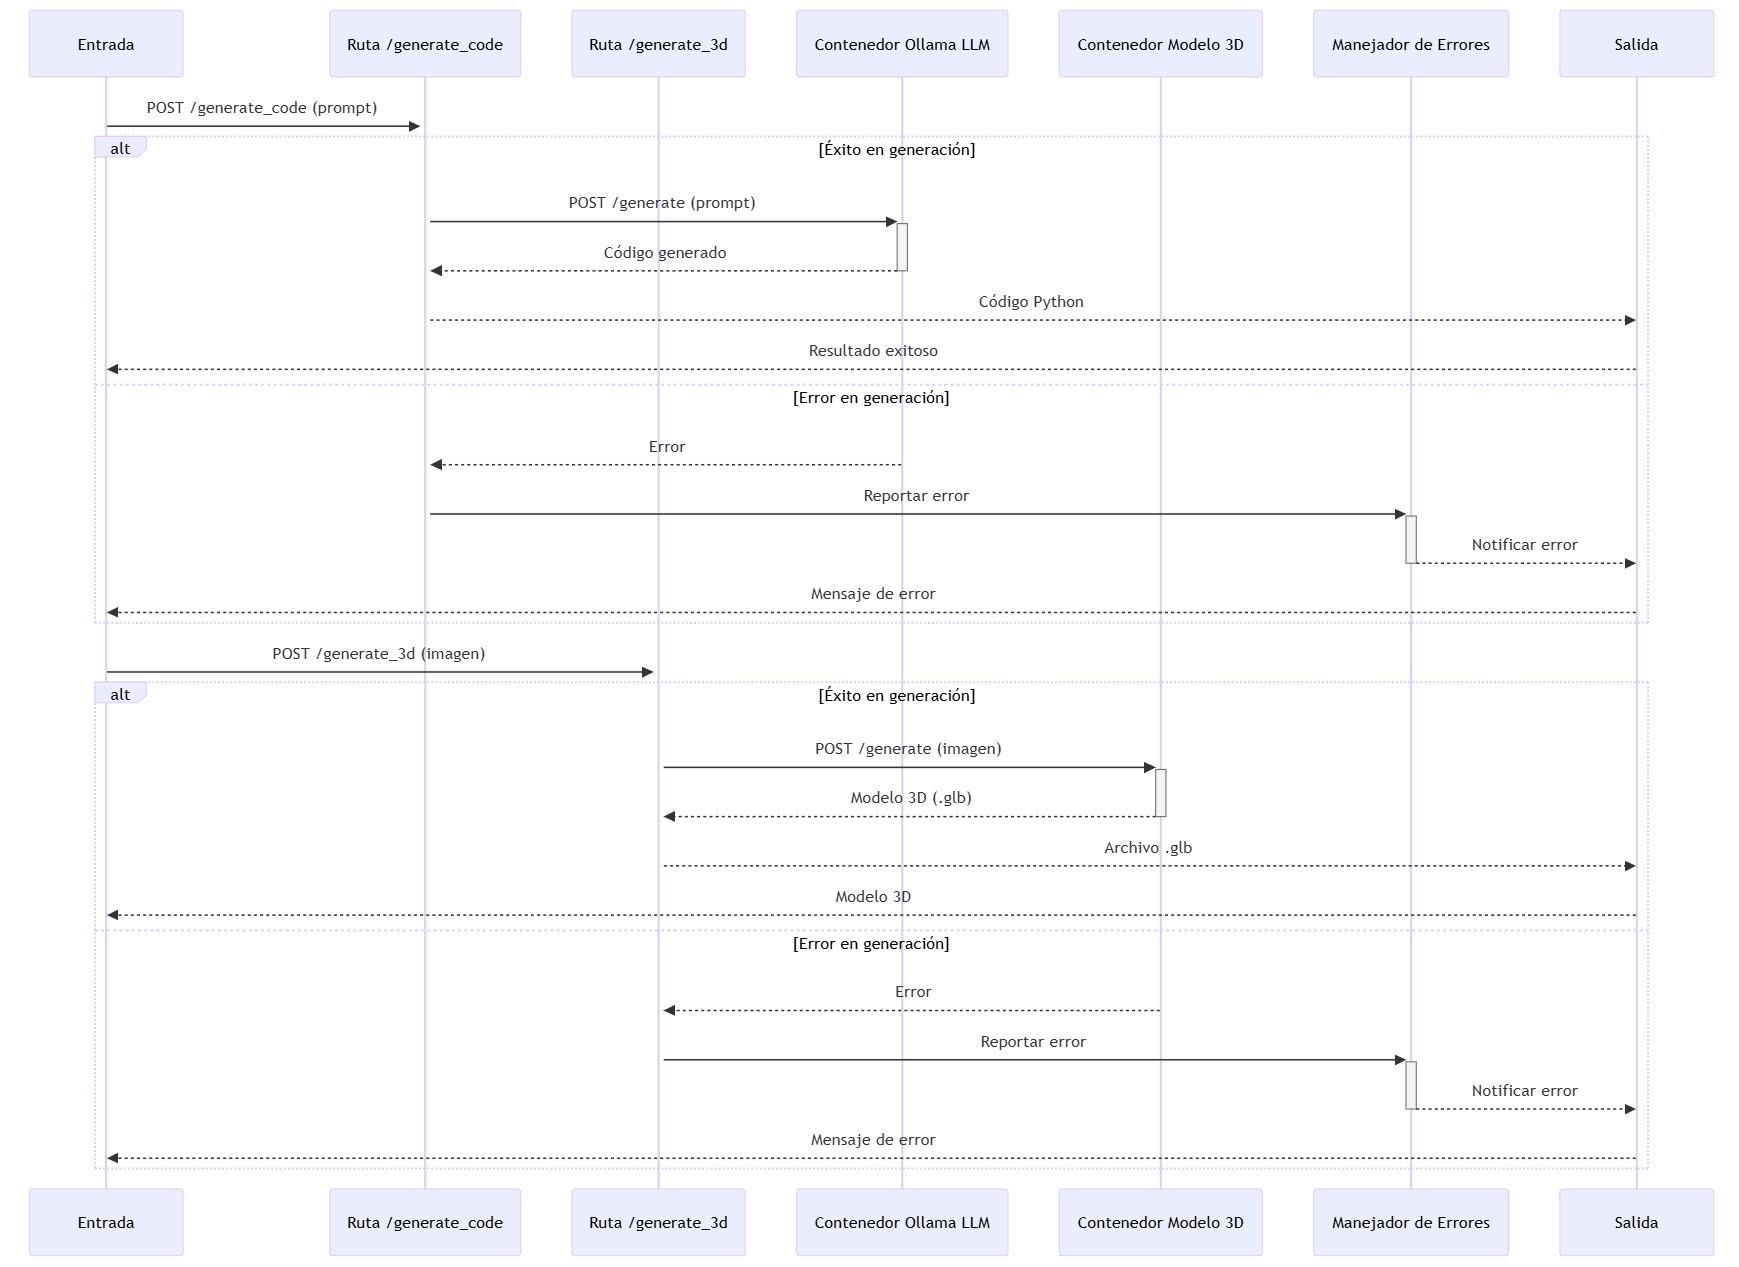
\includegraphics[width=1.1\textwidth]{figs/DiagramaSecuenciaAPI.png}
  \caption{Diagrama de secuencia de la API Nginx.}
  \label{fig:diagramaAPI2}
\end{figure}



La Figura~\ref{fig:diagramaMLLM1} representa el diagrama de componentes del contenedor que aloja el modelo LLM provisto por Ollama, concretamente utilizando la imagen correspondiente al modelo Dolphin-Mistral.
% Imagen diagrama componente 7
\begin{figure}[h!tp]
  \centering
  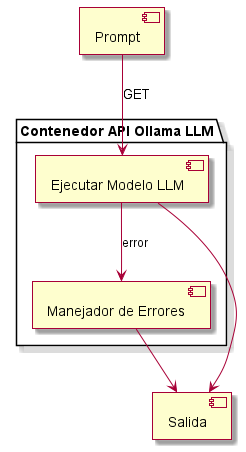
\includegraphics[width=0.4\textwidth]{figs/DiagramaComponentesMLLM.png}
  \caption{Diagrama de componentes del contenedor del modelo LLM.}
  \label{fig:diagramaMLLM1}
\end{figure}
Este componente es responsable de recibir los prompts textuales enviados por el proxy Nginx, obtenerlas mediante la API REST propia de Ollama, ejecutar el modelo LLM sobre dicha entrada, y generar como resultado una respuesta estructurada que incluye el código Python solicitado. Una vez completado el proceso de inferencia, la salida es reenviada a la API y el proxy para su posterior transmisión al add-on. En caso de producirse errores durante la ejecución del modelo, estos son capturados y redirigidos al módulo de notificación de errores, el cual se encarga de generar una respuesta adecuada que será igualmente retornada a través del proxy. El comportamiento detallado de este flujo, así como las interacciones entre componentes, se especifica en el diagrama de secuencia mostrado en la Figura~\ref{fig:diagramaMLLM2}.


% Imagen diagrama secuencia 7
\begin{figure}[h!tp]
  \centering
  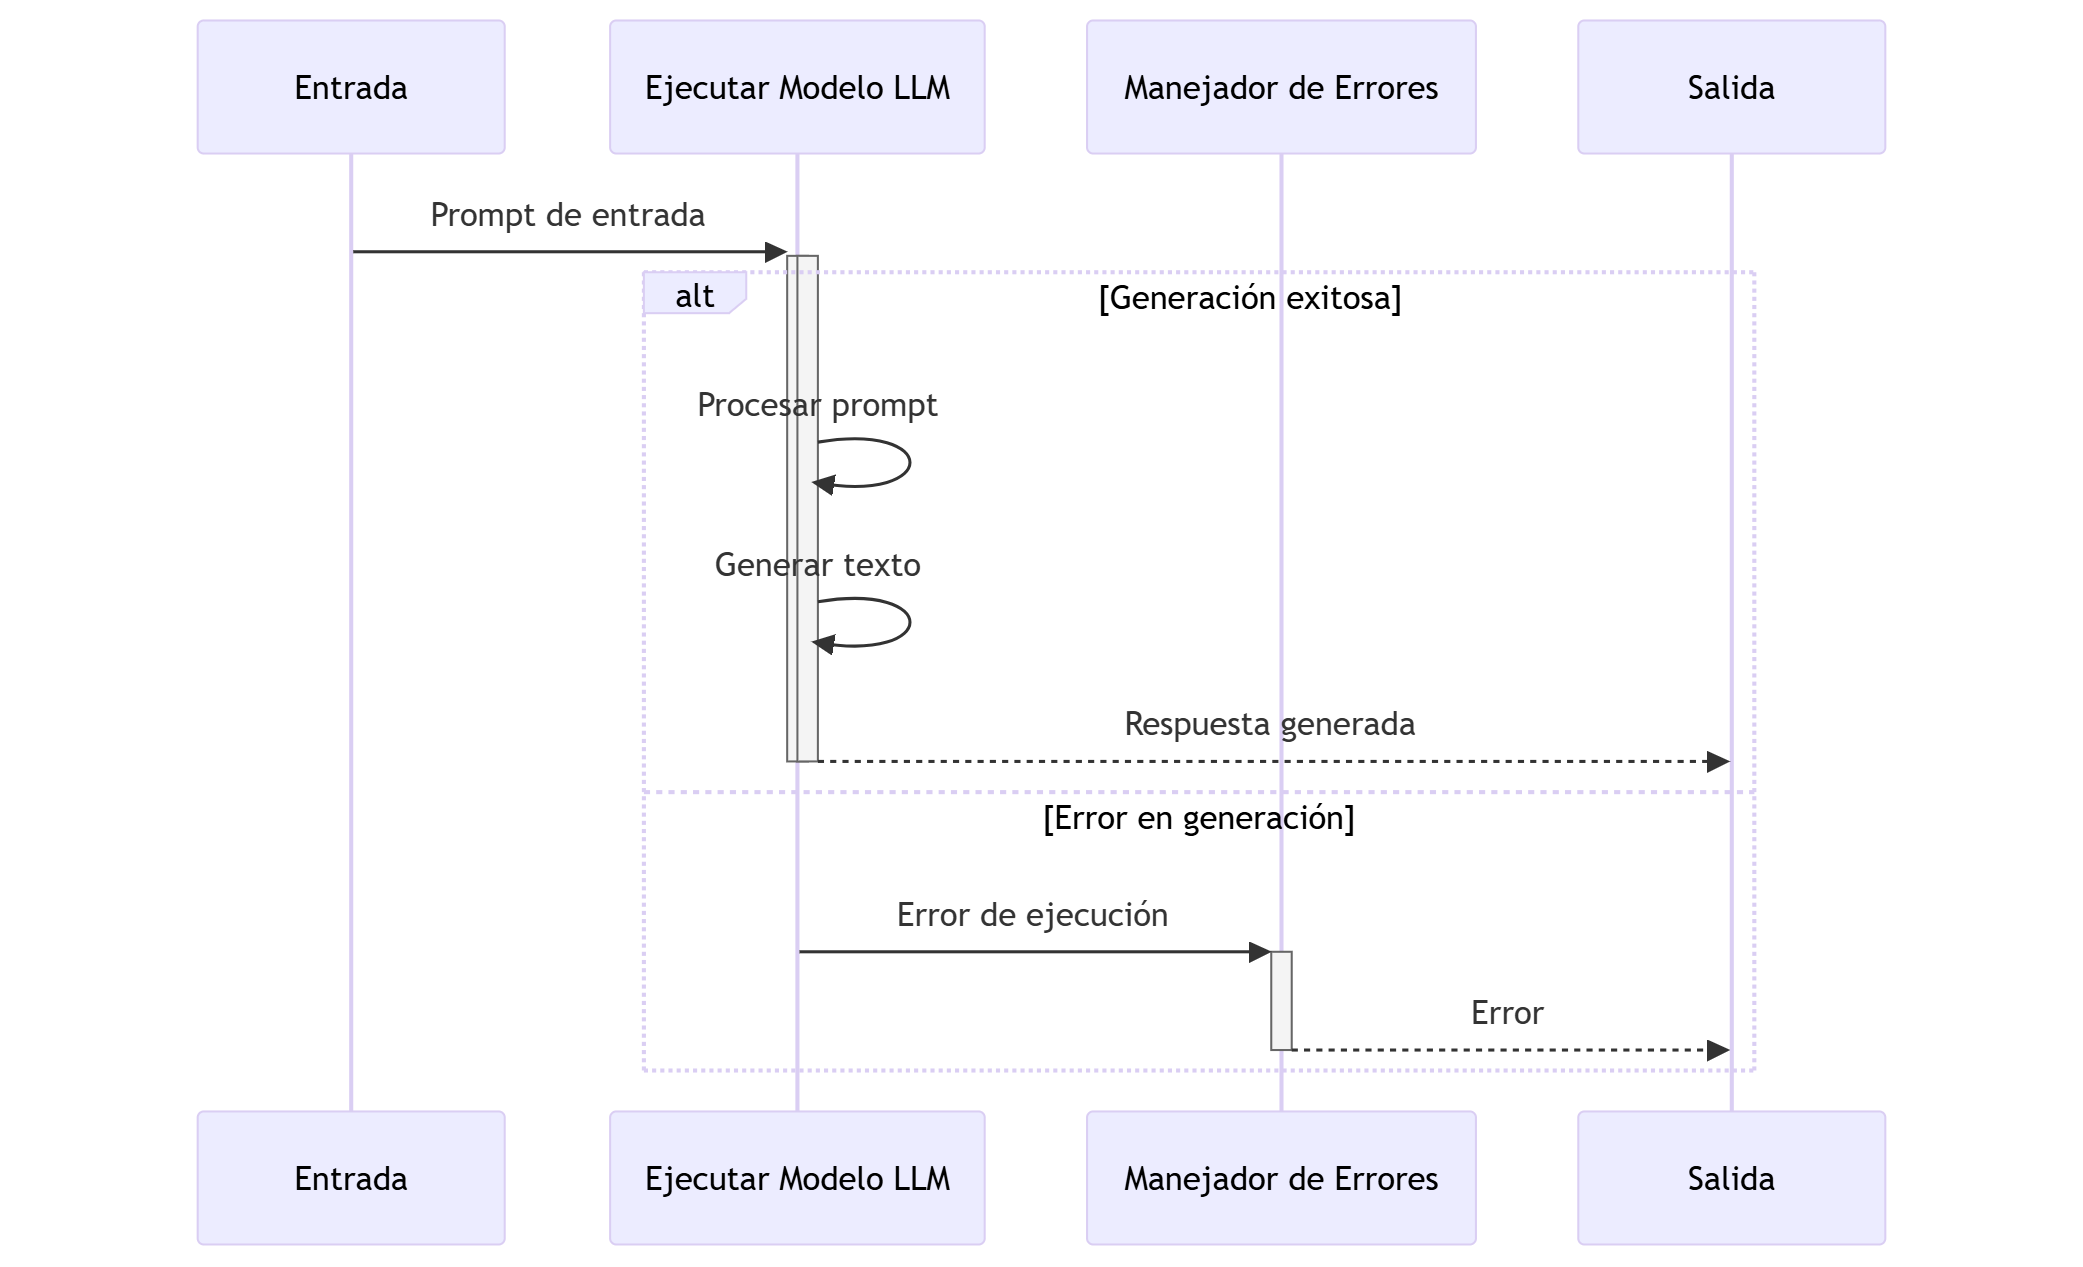
\includegraphics[width=1.0\textwidth]{figs/DiagramaSecuenciaMLLM.png}
  \caption{Diagrama de secuencia del contenedor del modelo LLM.}
  \label{fig:diagramaMLLM2}
\end{figure}



Como último componente del subsistema de infraestructura de servicios dockerizados y al mismo tiempo como subsistema final del proyecto, se presenta en la Figura~\ref{fig:diagramaMIA3D1} el diagrama de componentes correspondiente al contenedor del modelo de generación 3D mediante \gls{ia}. Este módulo está diseñado para recibir, a través del proxy Nginx, una imagen proporcionada por el add-on y procesarla mediante la API Flask custom del contenedor y utilizando una instancia personalizada del modelo TripoSR, especializado en reconstrucción tridimensional a partir de imágenes. Tras la ejecución del modelo, se genera una respuesta estructurada que contiene el modelo 3D del objeto presente en la imagen de entrada, el cual es enviado nuevamente a la API del contenedor y finalmente al proxy general para su posterior entrega al add-on de Blender. En caso de que se produzcan errores durante la ejecución del modelo TripoSR, estos son capturados por el sistema y gestionados por el módulo de notificación de errores, que transmite el mensaje correspondiente de vuelta a través del canal de salida. El funcionamiento detallado de este flujo se encuentra descrito en el diagrama de secuencia de la Figura~\ref{fig:diagramaMIA3D2}. Es importante señalar que tanto la API Flask como la imagen Docker de este contenedor de Docker y modelo de inteligencia artificial han sido desarrolladas de forma personalizada. Para ello, se ha empleado el lenguaje Python en la implementación de la API, así como un lenguaje específico de dominio (DSL) en la elaboración de los archivos de configuración de Docker.
% Imagen diagrama componente 8
\begin{figure}[h!tp]
  \centering
  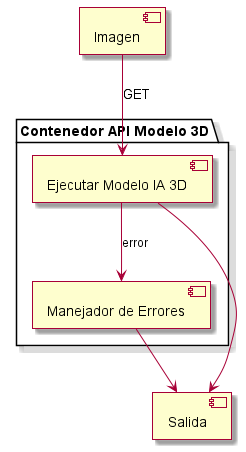
\includegraphics[width=0.4\textwidth]{figs/DiagramaComponentesMIA3D.png}
  \caption{Diagrama de componentes del contenedor del modelo IA 3D.}
  \label{fig:diagramaMIA3D1}
\end{figure}

% Imagen diagrama secuencia 8
\begin{figure}[h!tp]
  \centering
  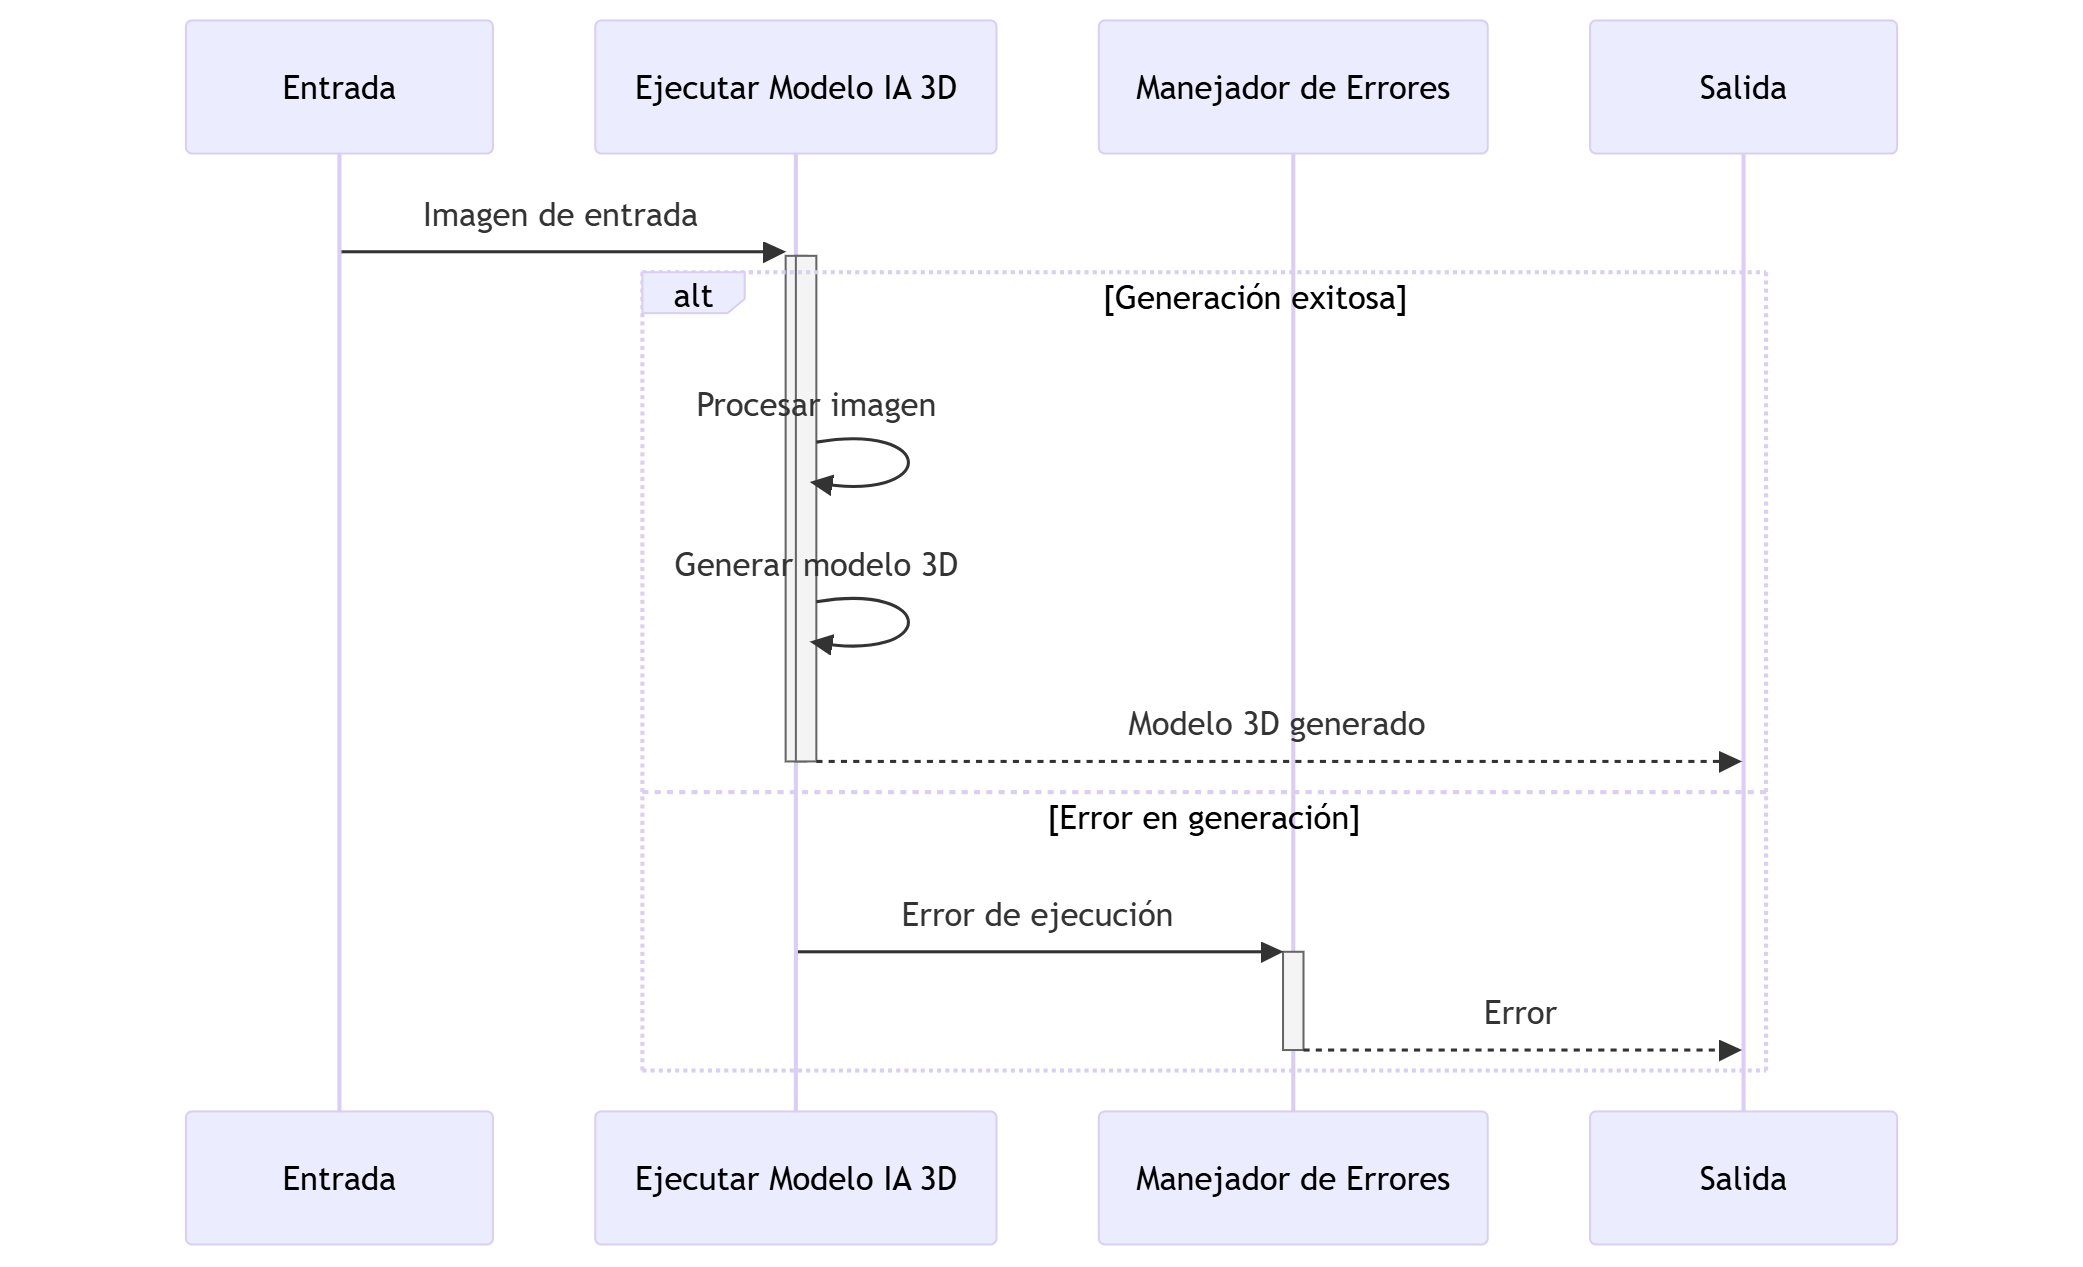
\includegraphics[width=1.0\textwidth]{figs/DiagramaSecuenciaMIA3D.png}
  \caption{Diagrama de secuencia del contenedor del modelo IA 3D.}
  \label{fig:diagramaMIA3D2}
\end{figure}



\section{Despliegue del sistema}
% En esta sección se debe presentar el diagrama de despliegue del sistema, que muestre la arquitectura física del sistema y cómo se distribuyen los componentes en los nodos físicos o virtuales que lo componen.
% En otras palabras, para cada componente principal del sistema se identifica en que servidor físico o virtual se va a ejecutar.

% Se puede definir un despligue de desarrollo (el despliegue que se tiene en el portátil mientras se trabaja), uno de producción (despliegue final o real) y uno de pruebas (lo más parecido posible al real).

En esta sección se expone la implementación y el despliegue completo del sistema, con especial énfasis en la configuración basada en Docker Compose, utilizada durante la fase de pruebas y validación funcional. La Figura~\ref{fig:diagramaDGS} muestra una visión general de la arquitectura de despliegue adoptada, diferenciando claramente los dos dispositivos clave involucrados en la operación del sistema.

% Imagen diagrama de despliegue general del sistema
\begin{figure}[h!tp]
  \centering
  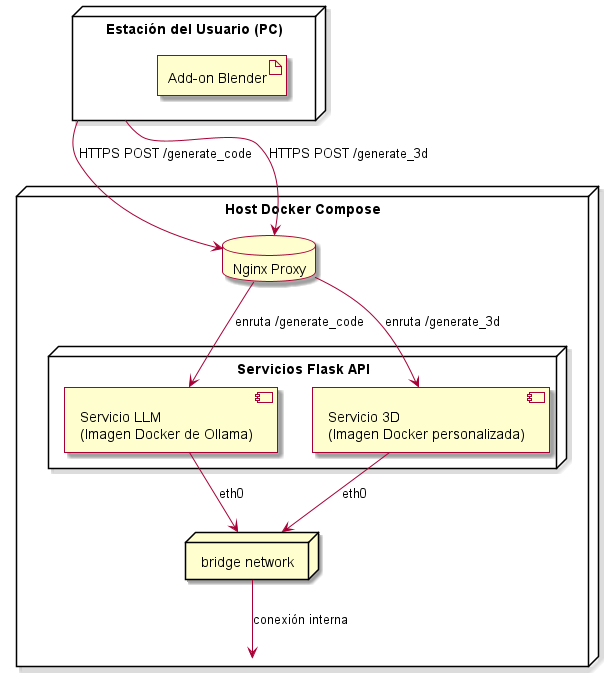
\includegraphics[width=0.8\textwidth]{figs/DiagramaDespliegueGeneral.png}
  \caption{Diagrama de despliegue general del sistema.}
  \label{fig:diagramaDGS}
\end{figure}

Por un lado, se encuentra el dispositivo local del usuario/a, en el que se instala el add-on para Blender, el cual actúa como interfaz principal y punto de interacción con los modelos de inteligencia artificial. Por otro lado, se encuentra la infraestructura en la nube (cloud), simulada en este proyecto mediante un entorno de contenedores Docker. Esta capa es responsable de la ejecución de los modelos de IA a través de un proxy Nginx que intermedia entre los distintos contenedores y las API de cada servicio.

La comunicación entre ambos componentes se realiza mediante un proxy de Nginx y las API REST de los modelos, que permite el envío de solicitudes HTTPS al servicio de Nginx y finalmente a la API del servicio alojada en Flask. Dado que todo el entorno se ejecuta en una única máquina física durante el desarrollo y las pruebas, todas las peticiones se dirigen a \verb|localhost| (127.0.0.1).

Una descripción más detallada del entorno de contenedores se presenta en la Figura~\ref{fig:diagramaDDC},
% Imagen diagrama de despliegue de Docker Compose
\begin{figure}[h!tp]
  \centering
  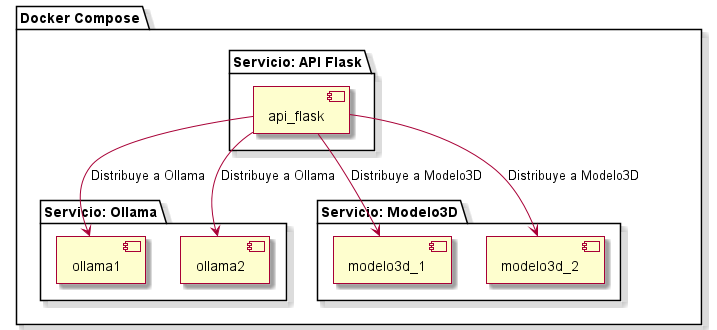
\includegraphics[width=0.8\textwidth]{figs/DiagramaDespliegueDockerCompose.png}
  \caption{Diagrama de despliegue local.}
  \label{fig:diagramaDDC}
\end{figure}
donde se observa que el nodo cloud, ejecutado sobre Docker, está compuesto por tres subcomponentes principales:

\begin{enumerate}
  \item \textbf{Contenedor de la API Nginx}: este módulo actúa como intermediario, recibiendo las solicitudes del add-on y redirigiéndolas al API REST del servicio correspondiente en función del tipo de petición recibida.
  \item \textbf{Contenedor de la API}: este módulo existe en cada contenedor de un modelo de IA recibe las solicitudes del proxy y las ejecuta en su modelo de IA correspondiente.
  \item \textbf{Servicio de modelos LLM (Ollama)}: encargado de procesar los prompts enviados por el usuario/a para generar código en Python. Este servicio se despliega con múltiples modelos LLM de forma concurrente, permitiendo la gestión simultánea de varias peticiones.
  \item \textbf{Servicio de modelado 3D}: responsable de la conversión de imágenes en objetos tridimensionales mediante modelos generativos 3D. Al igual que el anterior, este componente también admite múltiples instancias del modelo, lo que garantiza la capacidad de respuesta ante múltiples solicitudes concurrentes.
\end{enumerate}

Esta arquitectura modular basada en contenedores permite escalar los distintos servicios de manera independiente, además de facilitar el mantenimiento, la portabilidad y el despliegue del sistema en entornos distribuidos. La Figura \ref{fig:esbozoDespliegue} ilustra el esquema preliminar del despliegue en producción previsto para este sistema, que en esta ocasión se llevará a cabo localmente.

% Imagen esbozo
\begin{figure}[h!tp]
  \centering
  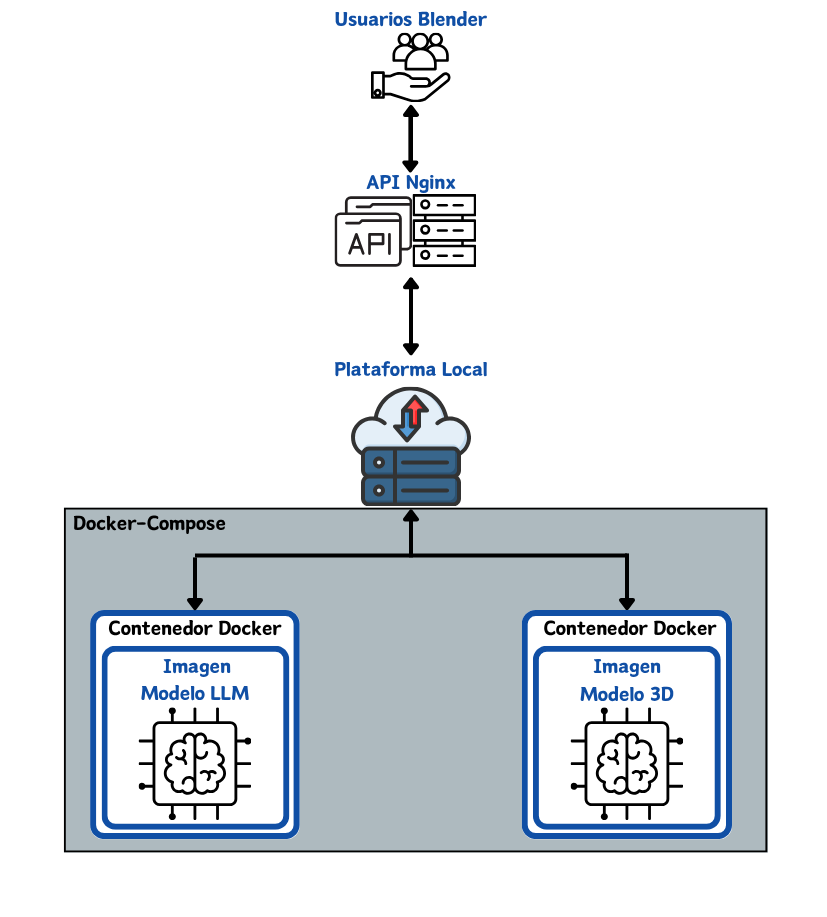
\includegraphics[width=0.8\textwidth]{figs/esbozoDespliegue.png}
  \caption{Esbozo del despliegue en producción del sistema.}
  \label{fig:esbozoDespliegue}
\end{figure}







\section{Wireframe de la pantalla del Add-on}

En esta sección, se presenta la Figura~\ref{fig:wireframeUI}, la cual ilustra el diseño del wireframe de la interfaz de usuario/a creada para el complemento de Blender denominado GenerativeCHAT, el cual ha sido diseñado para facilitar la interacción entre el usuario/a y los modelos de inteligencia artificial generativa integrados en el sistema. La interfaz se estructura en dos bloques funcionales principales: el Agente \gls{llm} y el Agente 3D, cada uno orientado a una tarea específica del flujo de trabajo.

En la parte superior se encuentra el Agente \gls{llm}, encargado de la generación automática de código Python adaptado al entorno de Blender. El usuario/a introduce una instrucción en lenguaje natural en el campo de entrada, y al activar la opción \emph{Generar código}, dicha instrucción es procesada por el modelo \gls{llm}. La respuesta es generada en forma de flujo continuo, lo que permite observar el proceso de respuesta de la \gls{ia}. Esta respuesta es representada en un campo de texto intermedio y en la pestaña de programación de Blender, también puede ser ejecutado el código resultante directamente dentro de Blender mediante el botón \emph{Ejecutar código}. Este mecanismo facilita una integración fluida entre el lenguaje natural y la automatización de tareas.

En la parte inferior, el Agente 3D permite al usuario/a generar modelos tridimensionales a partir de imágenes. A través del botón \emph{Cargar imagen}, se envía una imagen al modelo generativo 3D, el cual produce una reconstrucción volumétrica del contenido visual. Posteriormente, el modelo generado puede ser importado al entorno de Blender mediante la opción \emph{Cargar modelo} o exportado mediante \emph{Descargar modelo}.

% Imagen wireframe del diseño del add-on
\begin{figure}[h!tp]
  \centering
  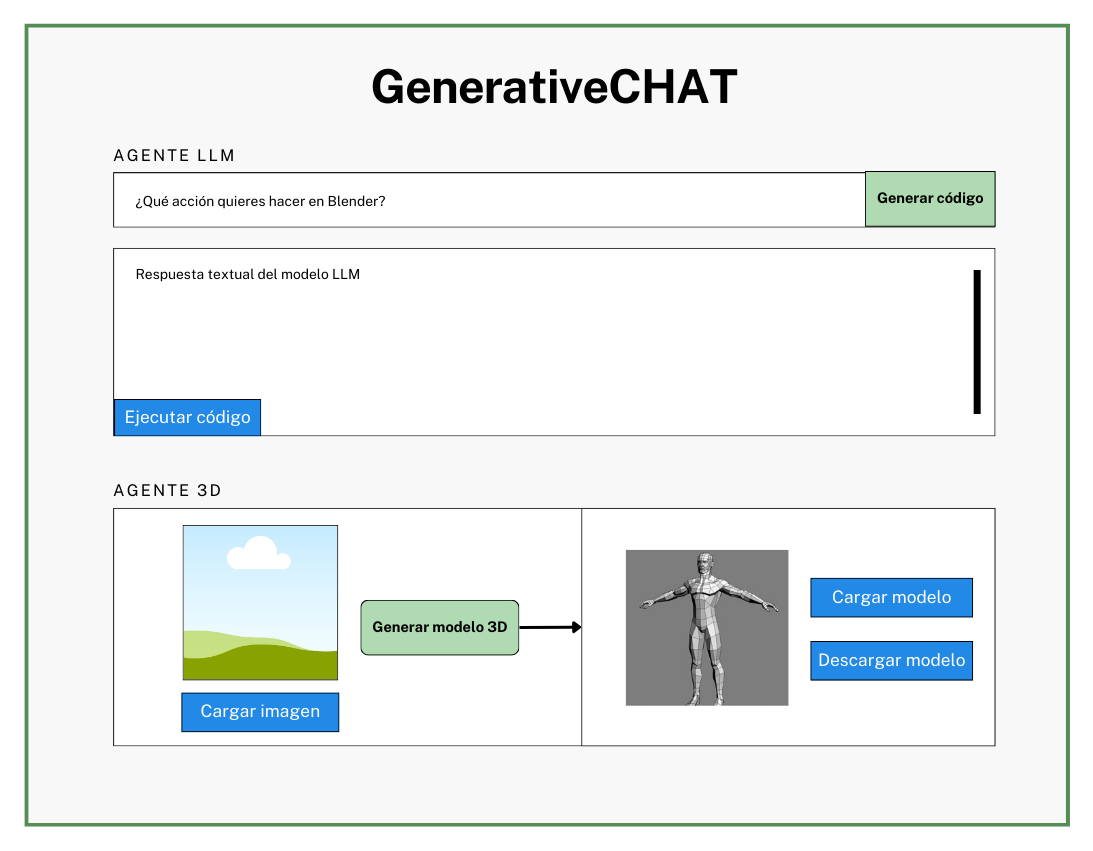
\includegraphics[width=0.8\textwidth]{figs/wireframeAddon.png}
  \caption{Wireframe del diseño del add-on.}
  \label{fig:wireframeUI}
\end{figure}

% En este caso se puede especificar el diagrama de clases final del diseño atendiendo al lenguaje de programación y a la tecnología seleccionada.
% Además será necesario, como mínimo, especificar el modelo físico de datos, en el lenguaje SQL propio de la base de datos relacional seleccionada, o el modelo de documentos, si se utiliza una base de datos NoSQL. 


\chapter{Implementación y pruebas}\label{ch:implementacion}
% % Contenidos del capítulo.
% Las secciones presentadas son orientativas y no representan
% necesariamente la organización que debe tener este capítulo.
Este capítulo tiene como objetivo detallar la implementación técnica de los distintos subsistemas que conforman el sistema, conforme a la arquitectura previamente definida. En primer lugar, se abordará la codificación e integración de los componentes pertenecientes a cada nodo funcional, siguiendo el orden lógico de ejecución dentro del flujo del sistema. A continuación, se describirá el funcionamiento global del sistema, incluyendo su proceso de despliegue local para la gestión de los servicios. Finalmente, se presentará el diseño y ejecución de un conjunto de pruebas funcionales y de rendimiento, orientadas a validar la estabilidad y eficiencia del sistema implementado.


\section{Implementación del subsistema del add-on de Blender}
En primer lugar, nos enfocaremos en la implementación del subsistema inicial, el cual corresponde al complemento específico de Blender que establecerá la conexión, a través de la interfaz gráfica, entre el usuario/a y los distintos servicios ofrecidos por el servidor de inteligencias artificiales. Además de facilitar esta conexión, el complemento desempeña otras funciones como la ejecución del código generado en la respuesta, la importación de imágenes, la exportación de modelos 3D, la carga de modelos 3D en la escena de Blender, la reversión de cualquier modificación realizada en la escena mediante el complemento y la visualización de cualquier error que ocurra durante su uso. Cabe destacar que la implementación de este subsistema se ha estructurado en tres etapas primeramente, la implementación de la interfaz gráfica y su correspondiente infraestructura secundaria, en segundo lugar, la implementación de la llamada para la generación del modelo 3D y finalmente, la llamada para la generación de texto del modelo \gls{llm}.
La Figura \ref{fig:instAddonBlender} muestra el panel de preferencias de Blender correspondiente a la versión 3.6 LTS, desde el cual se gestiona la instalación de complementos (add-ons). Para que el proceso de carga sea exitoso, es necesario empaquetar el conjunto de archivos del complemento en un archivo comprimido con extensión \verb|.zip|. Asimismo, se requiere que el archivo principal del complemento esté correctamente nombrado como \verb|__init__.py|, en conformidad con la estructura exigida por el sistema de detección e integración automática de Blender. Esta convención ha sido seguida en la implementación del presente trabajo.

% Imagen instalación add-on
\begin{figure}[h!tb]
  \centering
  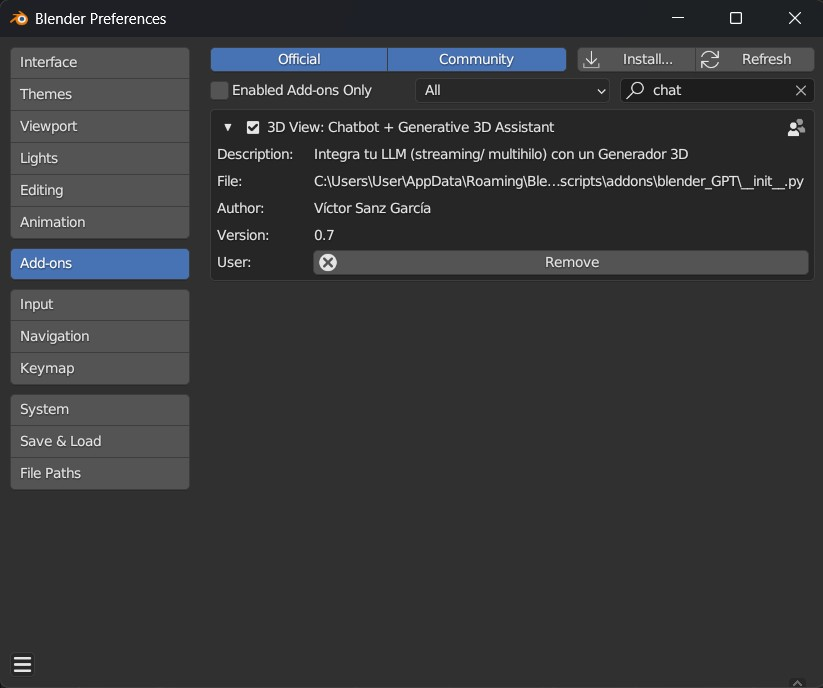
\includegraphics[width=0.8\textwidth]{figs/instalAddon.jpg}
  \caption{Instalación del add-on de Blender.}
  \label{fig:instAddonBlender}
\end{figure}

\subsection{Implementación de la interfaz de usuario y las herramientas auxiliares}
Para el desarrollo de la interfaz de usuario del complemento, se ha utilizado el lenguaje Python, aprovechando la API nativa de Blender, que permite la creación de add-ons personalizados mediante clases y métodos definidos en el módulo \verb|bpy|. En el Listado \ref{lst:panelAddon1} se presenta el código fuente completo de la interfaz, estructurado en un panel incorporado en la barra lateral de la vista 3D. Este panel se implementa mediante una subclase de \verb|bpy.types.Panel|, registrada con los atributos \verb|bl_space_type='VIEW_3D'| y \verb|bl_region_type='UI'|, lo que permite exponer controles gráficos vinculados a propiedades definidas en \verb|bpy.types.Scene|.

La interfaz se divide funcionalmente en dos secciones principales. La primera corresponde al Agente \gls{llm}, que incluye:
\begin{itemize}
  \item Un campo de texto para introducir el prompt del usuario/a.
  \item Un botón asociado que envía el prompt al modelo \gls{llm} para la generación de código.
  \item Un campo de texto para mostrar la respuesta generada por el modelo.
  \item Un botón adicional que ejecuta directamente el código recibido dentro del entorno de Blender.

        Además, una vez se recibe la respuesta, se activa automáticamente el panel de scripting de Blender, donde también se muestra el código generado.
\end{itemize}
La segunda sección está destinada al Agente 3D y contempla el flujo de generación de modelos tridimensionales a partir de imágenes. Esta parte incluye:
\begin{itemize}
  \item Un botón que abre el explorador de archivos para seleccionar la imagen de entrada.
  \item Un botón para enviar la imagen al modelo generativo 3D y recibir la reconstrucción.
  \item Una vez obtenida la respuesta, se habilitan dos botones adicionales, uno para importar el modelo 3D directamente en la escena de Blender y otro para exportarlo en formato \verb|.glb|, permitiendo al usuario/a elegir la ruta de descarga a través del sistema de archivos.
\end{itemize}
El panel del add-on se puede observar en la Figura \ref{fig:addonBlender}.

% Imagen add-on
\begin{figure}[h!tb]
  \centering
  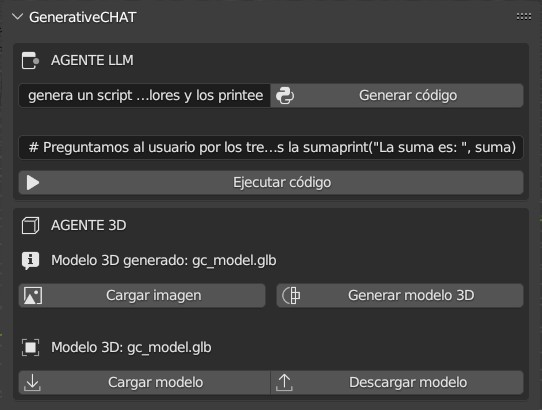
\includegraphics[width=0.8\textwidth]{figs/panelAddon.jpg}
  \caption{Interfaz de usuario del add-on de Blender.}
  \label{fig:addonBlender}
\end{figure}

Para la ejecución dinámica de código Python generado, se ha desarrollado un operador personalizado en Blender que accede al bloque de texto almacenado como propiedad en la escena. La ejecución se realiza mediante la función \verb|exec()| dentro del método \verb|execute(self, context)|, encapsulando el proceso en una estructura de control \verb|try/except| que permite capturar y reportar posibles errores mediante \verb|self.report|, sin comprometer la estabilidad ni bloquear la interfaz de usuario. La importación de imágenes se gestiona a través de otro operador que utiliza el selector de archivos \\(\verb|context.window_manager|), y una vez seleccionada la imagen, se carga en memoria con \verb|bpy.data.images.load()|. La ruta y el nombre del datablock correspondiente se almacenan en propiedades de escena para su reutilización, y se presenta una vista previa mediante \verb|layout.template_preview(img)| para validar visualmente la carga. En cuanto a la exportación de modelos 3D, se implementa un operador que invoca un diálogo de guardado, y dentro del método \verb|execute()| transfiere el archivo temporal (en formato \verb|.glb|) a la ruta de destino utilizando \verb|shutil.copy|. Este proceso también contempla el manejo de excepciones relacionadas con permisos o rutas inexistentes, notificando al usuario/a mediante los correspondientes mensajes de error. Para la carga de modelos 3D en la escena, se ha definido otro operador que verifica la validez de la ruta previamente almacenada y realiza la importación a través de \verb|bpy.ops.import_scene.gltf(filepath=...)| adecuado para el formato \verb|.glb|. Se implementan bloques \verb|try/except| tanto para informar errores como para confirmar el éxito del proceso. Las funcionalidades de reversión de cambios aprovechan el sistema de deshacer nativo de Blender, mediante la declaración \verb|bl_options = {'REGISTER', 'UNDO'}| en aquellos operadores que modifican el estado de la escena. Esto permite que cualquier acción pueda ser revertida mediante combinaciones estándar como Ctrl+Z. Durante todo el flujo, se emplea una propiedad de estado en la escena para mostrar mensajes persistentes de seguimiento por ejemplo, (Generando...) y (Error...), actualizados desde el hilo principal mediante \verb|bpy.app.timers.register| en casos donde se recurre a procesos asincrónicos como llamadas HTTP. Esto asegura que la interfaz de usuario permanezca reactiva, incluso durante operaciones de larga duración. Finalmente, todos los operadores implementan validaciones previas sobre las rutas y datos implicados, gestionan adecuadamente los nombres de los datablocks para evitar colisiones y realizan limpieza de recursos temporales cuando es necesario. Se han incluido además descripciones (\verb|bl_description|) y docstrings claras en cada clase, mejorando la usabilidad, la documentación interna y la detección de errores por parte del usuario/a durante la ejecución de tareas críticas como importación, exportación o ejecución de scripts generados dinámicamente.




\subsection{Implementación de la llamada al modelo 3D}
Para implementar la funcionalidad de llamada al modelo generativo 3D en el add-on de Blender, se ha diseñado un operador personalizado (ver Listado \ref{lst:panelAddon1}) que emplea un hilo secundario (thread) para realizar la solicitud HTTP al servicio de generación de modelos 3D desplegado en el puerto 5000 del localhost (\verb|http://127.0.0.1:5000/upload|) que se explica posteriormente en la implementación del subsistema del servidor, con el objetivo de mantener la interfaz de usuario no bloqueante durante el proceso. En el método \verb|execute()|, se lanza un \verb|threading.Thread| en modo daemon, encargado de ejecutar la función \verb|requests.post| con la imagen seleccionada como entrada. Dado que la API de Blender no es segura para operaciones multihilo, no se realiza ninguna modificación directa sobre \verb|bpy.data| ni \verb|bpy.context| desde este hilo. En su lugar, se emplea una estructura de cola (\verb|queue.Queue|) para transferir el resultado de la petición al hilo principal. La comunicación asincrónica se gestiona mediante el registro de una función de callback en \verb|bpy.app.timers.register|, la cual se ejecuta en el hilo principal cuando la respuesta esté disponible. Este callback evalúa si la respuesta HTTP ha sido satisfactoria: si es así, guarda el archivo \verb|.glb| generado en una ruta temporal (usando \verb|tempfile.gettempdir()|), actualiza la propiedad\\ \verb|scene.gc_model_path| y modifica el estado \verb|scene.gc_status| con un mensaje del tipo “Modelo generado: nombre.glb”. En caso de producirse errores durante la solicitud (por ejemplo, fallos de red, timeouts o respuestas mal formateadas), estos se capturan en el hilo secundario y se comunican al principal mediante la cola. El callback en el hilo principal ejecuta un bloque \verb|try/except| para gestionar estos errores, actualizando el estado de la escena (\verb|scene.gc_status = f"Error: {str(e)}"|) y notificando al usuario/a mediante \verb|self.report({'ERROR'}, ...)|, ya sea dentro del operador inicial o mediante un operador auxiliar de notificación. Esta arquitectura garantiza que todas las interacciones con la API de Blender se realicen exclusivamente en el hilo principal, respetando las restricciones de seguridad asociadas a su ejecución. Durante todo el proceso, el panel de interfaz de usuario refleja el estado del sistema mostrando el mensaje “Generando…” mientras la operación está en curso. Una vez el callback actualiza el estado, se habilitan dinámicamente los botones “Cargar modelo” y “Descargar modelo”, o en su defecto, se muestra un mensaje de error.



\subsection{Implementación de la llamada al modelo LLM}

El Listado \ref{lst:streamBotAddon} detalla la implementación de la petición al modelo de lenguaje LLM.
Esta implementación se basa en una función denominada \verb|chatbot(pmt, key)|, la cual construye y envía una solicitud HTTP de tipo POST con soporte para transmisión continua de datos (streaming) al punto de acceso local (\verb|http://127.0.0.1:11434/api/generate|) expuesto en el puerto 11434 del localhost, lo cual se detalla posteriormente en la implementación de la arquitectura del subsistema del servidor. El cuerpo de la solicitud contiene un objeto JSON que incluye tanto el mensaje del usuario/a como los parámetros de configuración del modelo, tales como la selección del modelo específico \\(\verb|"model": "dolphin-mistral:7b-v2.6-dpo-laser-q4_0"|) y la activación del modo de respuesta continua (\verb|"stream": true|). La respuesta del servidor se gestiona de forma iterativa utilizando \verb|response.iter_lines()|, lo que permite procesar fragmentos de texto en tiempo real conforme son recibidos, evitando así bloqueos durante la generación de contenido. Cada línea de la respuesta es tratada como una posible estructura JSON. Si se detecta la presencia del campo \verb|response|, el fragmento correspondiente se extrae y se transmite a una cola de procesamiento (\verb|queue.Queue|) mediante la instrucción \verb|q.put(chunk)|. Este flujo se encapsula en una función \verb|create_chat_bot|, que actúa como envoltorio para ejecutar \verb|chatbot| dentro de un hilo secundario. Esta estrategia multihilo permite invocar la función desde el operador de Blender sin interferir con el hilo principal de la interfaz gráfica.
En el hilo principal, se utiliza \verb|bpy.app.timers.register(process_queue)| para programar un temporizador que accede periódicamente a la cola, extrayendo los fragmentos generados y pasándolos a la función \verb|write_chat(chunk)|. Esta función acumula el contenido en una variable global, filtra mediante expresiones regulares los bloques de código Python delimitados, y los inserta en un datablock de texto dentro de Blender. Simultáneamente, se actualiza la propiedad \verb|scene.response| para reflejar el resultado filtrado en la interfaz de usuario. El manejo de errores en la interacción con el modelo \gls{llm} se gestiona mediante bloques \verb|try/except| en la función \verb|chatbot|, donde se detectan y capturan errores de red o fallos en la decodificación JSON. En estos casos, se genera un fragmento de texto con la descripción del error y se envía a la cola de hilos, lo que permite notificar al usuario/a desde el hilo principal.

% \newpage
% \captionsetup{type=listing}
% \captionof{listing}{Código python (streamchatbot.py) generador del stream del chatbot.}
% \label{lst:streamBotAddon}
% \begin{minted}[breaklines, fontsize=\small, linenos]{python}
%     import requests
%     import json

%     def is_json(myjson):
%         try:
%             json_object = json.loads(myjson)
%             return True
%         except ValueError as e:
%             return False

%     def create_chat_bot(prompt, key, q): 
%         for chunk in chatbot(prompt, key):
%             if chunk:
%                 q.put(chunk)

%     def chatbot(pmt, key):
%         url = "http://127.0.0.1:11434/api/generate"

%         data = {
%             "model": "dolphin-mistral:7b-v2.6-dpo-laser-q4_0",
%             "prompt": pmt,
%             "stream": True
%         }

%         print("\nTú:", pmt, end="\n\n")
%         print("Blender_GPT:", end=" ")

%         try:
%             response = requests.post(url, json=data, stream=True, timeout=900)
%             response.raise_for_status()

%             for line in response.iter_lines():
%                 if line:
%                     try:
%                         json_data = json.loads(line)
%                         if 'response' in json_data:
%                             yield json_data['response']
%                     except json.JSONDecodeError:
%                         continue

%         except Exception as e:
%             yield f"\nError: {str(e)}"
% \end{minted}

\newpage
\section{Implementación del subsistema del servidor de IAs}
En segundo lugar, se describe la implementación del subsistema correspondiente al servidor de inteligencia artificial, responsable de gestionar y enrutar las solicitudes provenientes del complemento de Blender. Para ello, se ha integrado un sistema de proxy inverso basado en Nginx, el cual actúa como componente central de orquestación y balanceo de carga, redirigiendo las peticiones entrantes hacia el contenedor correspondiente, en función del tipo de modelo requerido (modelo de lenguaje o modelo generativo 3D). La infraestructura completa ha sido desplegada mediante Docker Compose, utilizando un archivo de configuración específico que coordina todos los servicios involucrados. En el caso de los modelos de lenguaje, se han utilizado imágenes oficiales de Ollama con el modelo Dolphin-Mistral, cuya descarga e instalación se realiza de forma automatizada a través de un script en Bash. Este script prepara el modelo dentro de un volumen compartido de Docker, lo que permite que todos los contenedores de Ollama tengan acceso eficiente y consistente a los recursos del modelo \gls{llm}. En cuanto al modelo generativo 3D, se ha creado una imagen personalizada a partir de un Dockerfile adaptado, el cual gestiona la instalación de todas las dependencias requeridas, incluyendo bibliotecas descargadas y modificadas como torchmcubes. Cabe señalar que dicha biblioteca presentó problemas de instalación, tal como se describió en el estado del arte, los cuales fueron resueltos mediante modificaciones manuales durante el proceso de construcción del contenedor. La imagen del modelo 3D también incorpora una API desarrollada con el framework Flask, encargada de recibir las solicitudes del proxy y ejecutar el modelo de TripoSR. Además, se ha adaptado el archivo de ejecución de dicho modelo, eliminando la dependencia de la biblioteca Gradio utilizada en el proyecto original, dado que en esta implementación no se requiere una interfaz web, ya que la interacción con el sistema se realiza exclusivamente a través del add-on para Blender. Finalmente, la Figura \ref{fig:carpetasServ} muestra la organización estructural de los componentes del servidor, incluyendo la jerarquía de carpetas y la distribución de los archivos de configuración, scripts y recursos empleados en el entorno de despliegue.

% Imagen orden carpetas servidor
\begin{figure}[h!tb]
  \centering
  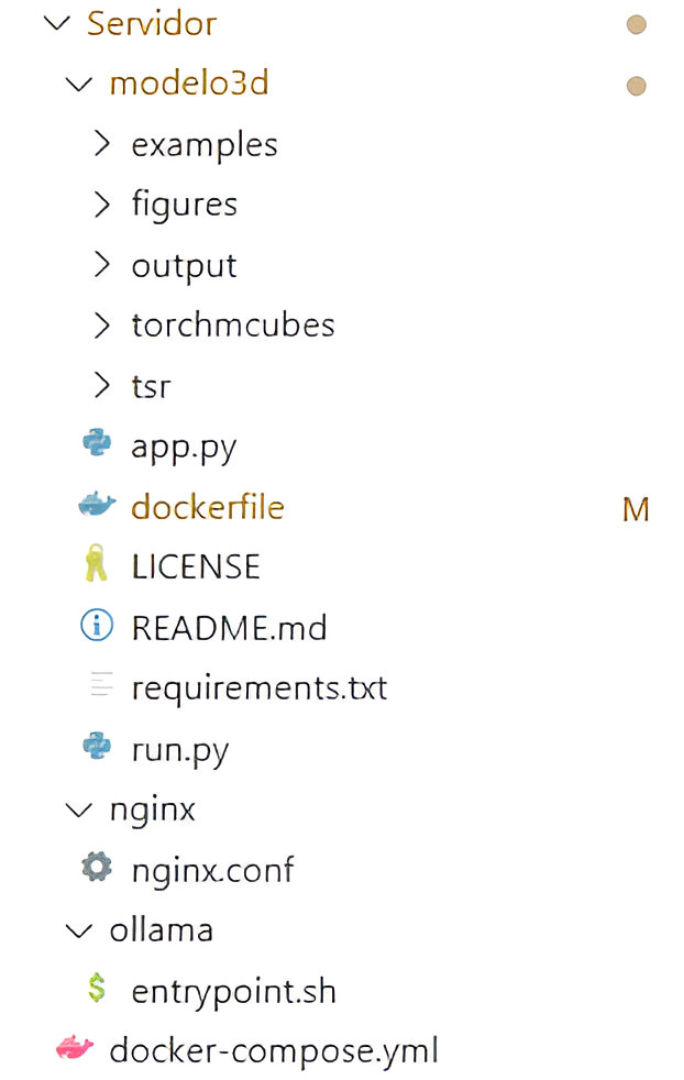
\includegraphics[width=0.4\textwidth]{figs/DistServidor.jpg}
  \caption{Distribución de las carpetas en el servidor.}
  \label{fig:carpetasServ}
\end{figure}


\newpage
\subsection{Implementación del modelo generativo LLM}
La puesta en marcha del modelo LLM Dolphin-Mistral proporcionado por Ollama se realiza mediante el script bash (\verb|entrypoint.sh|), mostrado en el Listado \ref{lst:scriptOllama}.

% % Bash
% \captionsetup{type=listing}
% \captionof{listing}{Script Bash (entrypoint.sh) de descarga e inicialización de Ollama y del modelo LLM.}
% \label{lst:scriptOllama}
% \begin{minted}[breaklines, fontsize=\small, linenos]{bash}
%     #!/bin/sh

%     # Inicia el servidor Ollama en segundo plano
%     /bin/ollama serve &

%     # Espera 20 segundos para que el servidor se inicie
%     sleep 20

%     # Verificar si el modelo está presente
%     MODEL_NAME="dolphin-mistral:7b-v2.6-dpo-laser-q4_0"
%     if ! ollama list | grep -q "$MODEL_NAME"; then
%         echo "Descargando el modelo..."

%         # Crear un lock file para evitar descargas concurrentes
%         LOCK_FILE="/root/.ollama/model_download.lock"
%         if [ ! -f "$LOCK_FILE" ]; then
%             touch "$LOCK_FILE"
%             ollama pull $MODEL_NAME
%             rm -f "$LOCK_FILE"
%         else
%             # Esperar a que otro contenedor complete la descarga
%             while [ -f "$LOCK_FILE" ]; do
%                 echo "Esperando que otro contenedor termine la descarga..."
%                 sleep 10
%             done
%         fi
%     fi

%     # Mantener el contenedor en ejecución
%     tail -f /dev/null
% \end{minted}

Este script cumple la función de inicializar de forma controlada el contenedor Docker correspondiente, dentro de una composición definida por Docker Compose. El script lanza el servidor de Ollama en segundo plano (\verb|/bin/ollama serve &|) y establece un tiempo de espera (\verb|sleep 20|) destinado a garantizar que el servicio se estabilice correctamente antes de continuar con los siguientes pasos. A continuación, el script comprueba mediante la interfaz de línea de comandos de Ollama (\verb|ollama list or grep -q "$MODEL_NAME"|) si el modelo \verb|dolphin-mistral:7b-v2.6-dpo-laser-q4-0| ya se encuentra disponible en el sistema, este modelo es la versión \verb|q4-0| menos cuantizada a la del modelo que se había planteado previamente que era \verb|dolphin-mistral:7b-v2.6-dpo-laser-q8-0| debido a que el modelo con \verb|q8-0| es uno más costoso computacionalmente y se planteo usar uno más liviano para obtener un mejor rendimiento. En caso de no detectarlo, se activa un mecanismo de control de concurrencia mediante un archivo de bloqueo (\verb|/root/.ollama/model_download.lock|). Este archivo actúa como semáforo para evitar descargas duplicadas en contextos donde múltiples contenedores podrían iniciarse de forma simultánea. Si el archivo ya existe, el contenedor entra en un bucle de espera activa hasta que el recurso quede liberado, en caso contrario, se crea el archivo, se descarga el modelo requerido (\verb|ollama pull $MODEL_NAME|) y se elimina el bloqueo una vez finalizada la operación. Este proceso está incorporado dentro del ecosistema de servicios a través de un proxy, como se ha descrito previamente, el cual redirecciona las solicitudes emitidas desde Blender hacia los contenedores que ya cuentan con el modelo preparado.


\subsection{Implementación del modelo generativo 3D}
La implementación del modelo generativo TripoSR se ha estructurado en un conjunto de componentes organizados jerárquicamente, tal como se muestra en la Figura \ref{fig:carpetasModel3D}. En primer lugar, se encuentran los directorios \verb|examples| y \verb|figures|, que contienen ejemplos ilustrativos proporcionados por el repositorio original. Estas carpetas incluyen tanto imágenes de entrada como modelos 3D de referencia generados, útiles para validar el comportamiento del modelo durante la fase de pruebas. A continuación, se destaca la carpeta \verb|output|, que tiene un papel central en el flujo de ejecución del servicio, ya que almacena el modelo tridimensional generado por el sistema. Este archivo es posteriormente devuelto al proxy y este al add-on de Blender. También se incluye el directorio correspondiente a la biblioteca \verb|torchmcubes|, la cual ha requerido modificaciones manuales en su proceso de instalación debido a problemas de compatibilidad, como se explicó previamente. La carpeta \verb|tsr| contiene los archivos compilados necesarios para la ejecución del modelo, incluyendo los pesos preentrenados y los módulos auxiliares que conforman el núcleo funcional de TripoSR. En la raíz del proyecto, se localiza el archivo \verb|app.py|, que define la API construida con Flask encargada de recibir las solicitudes, ejecutar el modelo y retornar la salida correspondiente. El entorno se completa con el archivo \verb|Dockerfile|, el cual describe las instrucciones necesarias para la construcción de la imagen del servicio 3D dentro del contenedor. Este archivo hace uso del documento \verb|requirements.txt|, que especifica las dependencias del proyecto y permite su instalación automatizada durante el proceso de build, cuyo contenido se muestra en el Listado \ref{lst:dependencias3D}. Finalmente, el archivo \verb|run.py| contiene el script principal en Python que lanza la ejecución del modelo TripoSR y coordina la generación del modelo tridimensional a partir de la imagen de entrada.

% Imagen orden carpetas modelo3d
\begin{figure}[h!tb]
  \centering
  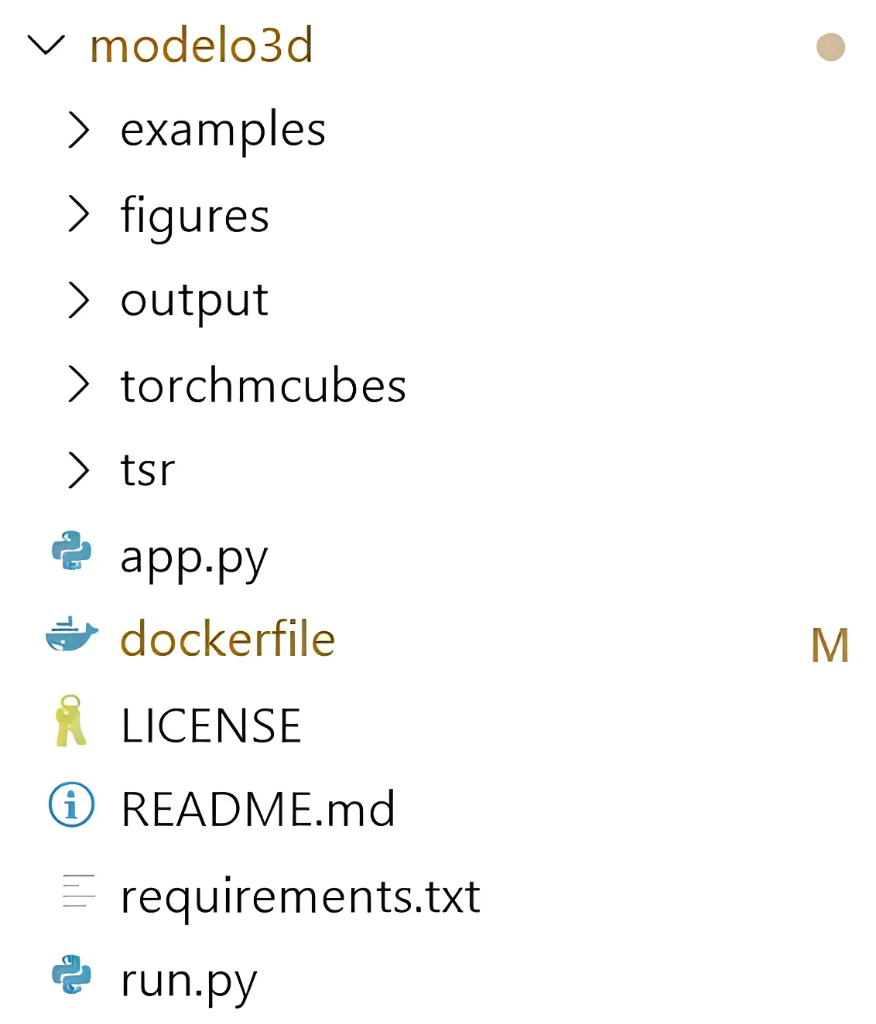
\includegraphics[width=0.4\textwidth]{figs/DistModelo3D.png}
  \caption{Distribución de las carpetas en el modelo 3D.}
  \label{fig:carpetasModel3D}
\end{figure}

% \newpage % Quitar cuando esté referenciado
% % Imagen requeriments.txt
% \captionsetup{type=listing}
% \captionof{listing}{Archivo (requirements.txt) de dependencias del modelo 3D.}
% \label{lst:dependencias3D}
% \begin{minted}[breaklines, fontsize=\small, linenos]{text}
%     flask
%     flask-cors
%     onnxruntime
%     gunicorn
%     omegaconf==2.3.0
%     Pillow==10.1.0
%     einops==0.7.0
%     transformers==4.35.0
%     trimesh==4.0.5
%     rembg
%     huggingface-hub
%     imageio[ffmpeg]
% \end{minted}

El Listado \ref{lst:appAPI3d} muestra el código de \verb|app.py| que se encarga de implementar el servicio REST para la inferencia del modelo generativo 3D TripoSR utilizando el framework Flask, actuando como mediador entre el proxy inverso Nginx y el motor de procesamiento 3D.
Los datos de entrada son gestionados a través del endpoint \verb|/upload|, el cual está configurado con el decorador \verb|@app.route('/upload', methods=['POST'])| y se utiliza para recibir archivos binarios enviados desde el add-on de Blender mediante \verb|request.files['image']|. Tras recibir la imagen, esta se pasa a la función \verb|generate_geometry(image_data)|, que se importa del script \verb|run.py|, para ejecutar el modelo TripoSR, produciendo como salida una malla en formato GLB. El archivo resultante se almacena temporalmente en el directorio \verb|output/0/|. La entrega del archivo generado al cliente se realiza mediante la función \verb|send_file(...)|, configurada con el tipo MIME \verb|model/gltf-binary| y encabezados apropiados para su correcta interpretación en Blender. Para permitir la interoperabilidad entre dominios dentro del entorno orquestado, se habilitan las políticas CORS mediante la instrucción \verb|flask_cors.CORS(app)|, lo que posibilita el acceso al servicio desde el proxy Nginx sin restricciones de origen y una simplificación del servicio a un único punto de entrada \verb|/upload|, reduciendo la complejidad estructural y minimizando la latencia. El servicio se expone en la dirección \verb|0.0.0.0| mediante \verb|app.run(host='0.0.0.0')|, lo que permite su correcta integración en el sistema de contenedores desplegado con Docker y su comunicación directa con el proxy. Por otro lado, el código Python del Listado \ref{lst:runAPI3d} es el código que ejecuta al modelo y incluye varias adaptaciones respecto al repositorio original de TripoSR, entre las cuales destaca la eliminación de la interfaz web desarrollada con Gradio, como se mencionó anteriormente.

% % Código API modelo3d
% \captionsetup{type=listing}
% \captionof{listing}{Código python (app.py) de la API Flask del modelo 3D.}
% \label{lst:appAPI3d}
% \begin{minted}[breaklines, fontsize=\small, linenos]{python}
%     from run import generate_geometry
%     from flask import Flask, request, send_file
%     from flask_cors import CORS
%     import os
%     import time

%     app = Flask(__name__)
%     CORS(app)

%     def check_file_existence(directory, filename):
%         """Function to check if a file exists in a directory."""
%         return os.path.exists(os.path.join(directory, filename))

%     @app.route('/upload', methods=['POST'])
%     def upload_file():
%         if 'image' in request.files:
%             image = request.files['image']
%             directory = 'output/0'
%             filename_mesh = 'mesh.glb'

%             # Lee los datos binarios de la imagen
%             image_data = image.read()
%             generate_geometry(image_data)  # Pasa los datos binarios

%             return send_file(os.path.join(directory, filename_mesh), as_attachment=True, mimetype='model/gltf-binary')
%         else:
%             return 'No image provided', 400

%     if __name__ == '__main__':
%         app.run(host='0.0.0.0')
% \end{minted}

% % Código modelo3d adaptado
% \captionsetup{type=listing}
% \captionof{listing}{Código python (run.py) que ejecuta el modelo 3D adaptado.}
% \label{lst:runAPI3d}
% \begin{minted}[breaklines, fontsize=\small, linenos]{python}
%     import argparse
%     import logging
%     import os
%     import time

%     import numpy as np
%     import rembg
%     import torch
%     from PIL import Image
%     from io import BytesIO

%     from tsr.system import TSR
%     from tsr.utils import remove_background, resize_foreground, save_video

%     def generate_geometry(image_web):
%         class Timer:
%             def __init__(self):
%                 self.items = {}
%                 self.time_scale = 1000.0  # ms
%                 self.time_unit = "ms"

%             def start(self, name: str) -> None:
%                 if torch.cuda.is_available():
%                     torch.cuda.synchronize()
%                 self.items[name] = time.time()
%                 logging.info(f"{name} ...")

%             def end(self, name: str) -> float:
%                 if name not in self.items:
%                     return
%                 if torch.cuda.is_available():
%                     torch.cuda.synchronize()
%                 start_time = self.items.pop(name)
%                 delta = time.time() - start_time
%                 t = delta * self.time_scale
%                 logging.info(f"{name} finished in {t:.2f}{self.time_unit}.")

%         timer = Timer()

%         logging.basicConfig(
%             format="%(asctime)s - %(levelname)s - %(message)s", level=logging.INFO
%         )

%         input_image = image_web      #"examples/chair.png"
%         output_dir = "output/"
%         device = "cuda:0"   #"cpu"
%         pretrained = "stabilityai/TripoSR"
%         chunksize = 8192
%         noremove_bg = False
%         foreground = 0.85
%         resolution = 256
%         model_format = "glb"    #"obj"
%         render_store = False

%         os.makedirs(output_dir, exist_ok=True)

%         if not torch.cuda.is_available():
%             device = "cpu"

%         timer.start("Initializing model")
%         model = TSR.from_pretrained(
%             pretrained,
%             config_name="config.yaml",
%             weight_name="model.ckpt",
%         )
%         model.renderer.set_chunk_size(chunksize)
%         model.to(device)
%         timer.end("Initializing model")

%         timer.start("Processing images")
%         images = []

%         if noremove_bg:
%             rembg_session = None
%         else:
%             rembg_session = rembg.new_session()

%         if noremove_bg:
%             image = np.array(Image.open(BytesIO(input_image)).convert("RGB"))
%         else:
%             image = remove_background(Image.open(BytesIO(input_image)), rembg_session)
%             image = resize_foreground(image, foreground)
%             image = np.array(image).astype(np.float32) / 255.0
%             image = image[:, :, :3] * image[:, :, 3:4] + (1 - image[:, :, 3:4]) * 0.5
%             image = Image.fromarray((image * 255.0).astype(np.uint8))
%             if not os.path.exists(os.path.join(output_dir, str(0))):
%                 os.makedirs(os.path.join(output_dir, str(0)))
%             image.save(os.path.join(output_dir, str(0), f"input.png"))
%         images.append(image)
%         timer.end("Processing images")

%         for i, image in enumerate(images):
%             logging.info(f"Running image {i + 1}/{len(images)} ...")

%             timer.start("Running model")
%             with torch.no_grad():
%                 scene_codes = model([image], device=device)
%             timer.end("Running model")

%             if render_store:
%                 timer.start("Rendering")
%                 render_images = model.render(scene_codes, n_views=30, return_type="pil")
%                 for ri, render_image in enumerate(render_images[0]):
%                     render_image.save(os.path.join(output_dir, str(i), f"render_{ri:03d}.png"))
%                 save_video(
%                     render_images[0], os.path.join(output_dir, str(i), f"render.mp4"), fps=30
%                 )
%                 timer.end("Rendering")

%             timer.start("Exporting mesh")
%             meshes = model.extract_mesh(scene_codes, resolution=resolution)
%             meshes[0].export(os.path.join(output_dir, str(i), f"mesh.{model_format}"))
%             timer.end("Exporting mesh")
% \end{minted}


El archivo \verb|Dockerfile| que aparece en el Listado \ref{lst:dockerfileM3D} establece una estrategia de construcción estructurada para generar una imagen personalizada del modelo TripoSR, abordando múltiples desafíos técnicos asociados al despliegue de entornos de inferencia basados en inteligencia artificial dentro de arquitecturas contenerizadas. La imagen se basa en la distribución \verb|python:3.8-slim|, seleccionada por su equilibrio entre ligereza y soporte funcional, permitiendo reducir significativamente el tamaño del contenedor sin comprometer su compatibilidad con las bibliotecas requeridas.
% \newpage
% % Dockerfile modelo3d
% \captionsetup{type=listing}
% \captionof{listing}{Dockerfile de la imagen de Docker del servicio del modelo 3D.}
% \label{lst:dockerfileM3D}
% \begin{minted}[breaklines, fontsize=\small, linenos]{dockerfile}
%     # Utiliza una imagen base de Python
%     FROM python:3.8-slim

%     # Establece el directorio de trabajo en el contenedor
%     WORKDIR /app

%     # Copia los archivos de la aplicación Flask al contenedor
%     COPY . /app

%     # Actualiza setuptools y luego instala las dependencias de Python
%     RUN pip install --upgrade setuptools && pip install -r requirements.txt && pip install torch torchvision torchaudio -f https://download.pytorch.org/whl/torch_stable.html

%     # Cambia al directorio del repositorio
%     WORKDIR /app/torchmcubes

%     RUN apt-get update && \
%         apt-get install -y g++ ninja-build && \
%         apt-get clean && \
%         rm -rf /var/lib/apt/lists/*

%     # Ejecuta el script de Python que genera la carpeta y el archivo .pyd
%     RUN python setup.py build_ext -i

%     # Mueve los archivos generados a la carpeta de librerías de Python
%     RUN mv torchmcubes /usr/local/lib/python3.8/site-packages/torchmcubes && \
%         mv build/lib.linux-x86_64-cpython-38/
%         torchmcubes_module.cpython-38-x86_64-linux-gnu.so 
%         /usr/local/lib/python3.8/site-packages/

%     WORKDIR /app

%     RUN rm -rf torchmcubes

%     # Expone el puerto en el que se ejecutará la aplicación Flask
%     EXPOSE 5000

%     # Ejecuta la aplicación Flask con Gunicorn para producción
%     CMD ["gunicorn", "-b", "0.0.0.0:5000", "--timeout", "1000", "app:app"]
% \end{minted}
El proceso de instalación de dependencias se ejecuta de manera controlada, comenzando con la actualización del gestor de paquetes \verb|setuptools|, seguida de la incorporación de las librerías especificadas en \verb|requirements.txt| y la inclusión explícita de los paquetes de PyTorch (\verb|torch|, \verb|torchvision|, \verb|torchaudio|) a través de binarios precompilados, con el objetivo de evitar compilaciones locales que incrementarían el tiempo de construcción y el tamaño de la imagen. Una parte crítica del proceso consiste en la integración manual de bibliotecas que presentan incompatibilidades documentadas, como \verb|torchmcubes|. Para solventar dichas incidencias, se incorpora una fase de compilación directa empleando herramientas del sistema (\verb|g++|, \verb|ninja-build|) y la instrucción \verb|python setup.py build_ext -i|, tras lo cual se reubica la biblioteca compilada en el directorio correspondiente de paquetes de Python, asegurando su correcto enlace durante la ejecución del modelo. Posteriormente, se lleva a cabo una fase de depuración del entorno mediante la eliminación de los archivos fuente y directorios intermedios utilizados durante la compilación, con el fin de minimizar tanto el tamaño final de la imagen como su superficie de exposición. Finalmente, el despliegue del servicio se configura para su ejecución bajo un entorno productivo utilizando el servidor WSGI Gunicorn, expuesto en la dirección \verb|0.0.0.0:5000|, y con un parámetro de espera extendido (\verb|timeout|) fijado en 1000 segundos. Esta configuración está orientada a garantizar la tolerancia a procesos computacionalmente intensivos propios de la generación 3D.




\subsection{Implementación y despliegue del servidor con Docker-Compose y Nginx}
El proceso de despliegue del servidor requiere la activación previa del entorno de ejecución Linux proporcionado por \gls{wsl2}, seguido del inicio manual del servicio Docker mediante la instrucción \verb|/etc/init.d/docker start|. Una vez iniciado el servicio, es necesario acceder al directorio del proyecto que contiene el archivo \verb|docker-compose.yml|, desde donde se ejecuta el comando \verb|docker-compose up -d --build --scale ollama=2 --scale modelo3d=2|. Este comando lanza el proceso de construcción y despliegue de los contenedores en segundo plano (\verb|-d|), fuerza la reconstrucción de las imágenes involucradas (\verb|--build|) y escala explícitamente el número de instancias del servicio \verb|ollama| y del servicio \verb|modelo3d| a dos contenedores cada uno (\verb|--scale|), permitiendo una mayor concurrencia en la atención de solicitudes por parte de los modelos de inteligencia artificial. La correcta ejecución de estas instrucciones puede observarse en las Figuras \ref{fig:despliegueServer1}, \ref{fig:despliegueServer2}, \ref{fig:despliegueServer3} y \ref{fig:despliegueServer4}, que documentan visualmente el estado del sistema tras la inicialización. Para la orquestación completa del entorno contenerizado se han utilizado, además del archivo \verb|docker-compose.yml|, los parámetros de configuración definidos en \verb|nginx.conf|, que permiten gestionar tanto el direccionamiento interno de las solicitudes como el balanceo de carga entre servicios concurrentes.

% Imagen despliegue docker
\begin{figure}[h!tb]
  \centering
  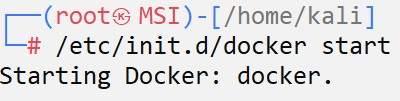
\includegraphics[width=0.3\textwidth]{figs/initDocker.jpg}
  \caption{Comando de inicio Docker en el entorno linux.}
  \label{fig:despliegueServer1}
\end{figure}

% Imagen despliegue servidor
\begin{figure}[h!tb]
  \centering
  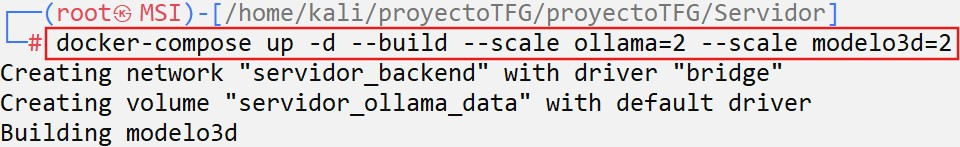
\includegraphics[width=0.7\textwidth]{figs/initServer.jpg}
  \caption{Comando de inicio Docker-Compose en el entorno linux.}
  \label{fig:despliegueServer2}
\end{figure}

% Imagen despliegue servidor
\begin{figure}[h!tb]
  \centering
  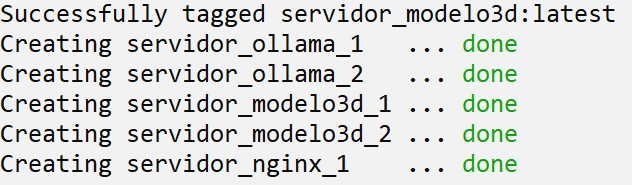
\includegraphics[width=0.5\textwidth]{figs/initServer2.jpg}
  \caption{Resultado del inicio del Docker-Compose en el entorno linux.}
  \label{fig:despliegueServer3}
\end{figure}

% Imagen despliegue servidor
\begin{figure}[h!tb]
  \centering
  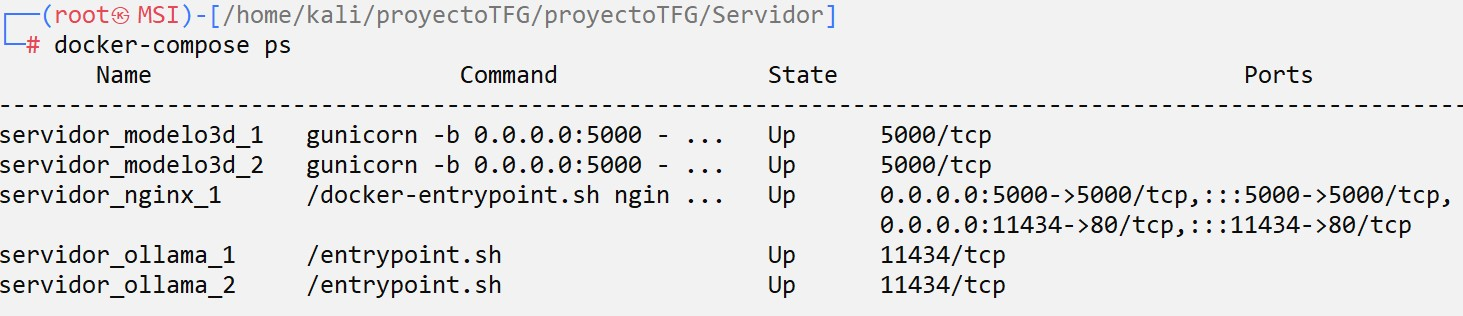
\includegraphics[width=1.0\textwidth]{figs/initServer3.jpg}
  \caption{Verificación del estado del servidor mediante docker-compose ps.}
  \label{fig:despliegueServer4}
\end{figure}


El archivo \verb|docker-compose.yml| que se muestra en el Listado \ref{lst:composeServidor} especifica la arquitectura de servicios que conforman el entorno de peticiones y sus componentes auxiliares, utilizando la versión 3.8 de la especificación de Docker Compose como base para la definición de recursos y configuraciones. Dentro de esta estructura, se declara un servicio denominado \verb|ollama|, basado en la imagen oficial \verb|ollama/ollama|, al cual se le asigna un volumen persistente denominado \verb|ollama_data|, montado en la ruta \verb|/root/.ollama|. Este volumen permite conservar tanto los modelos de lenguaje como sus metadatos, asegurando su disponibilidad entre reinicios del contenedor. El arranque del servicio se gestiona mediante un script personalizado (\verb|./ollama/entrypoint.sh|), cuyo propósito es garantizar la correcta inicialización del demonio responsable de ejecutar el modelo LLM al momento de levantar la instancia del contenedor. La red utilizada en el despliegue se define como \verb|backend|, empleando el controlador \verb|bridge| con el objetivo de aislar el tráfico de datos interno entre servicios, sin exponer directamente sus puertos al sistema anfitrión, lo que incrementa la seguridad de la infraestructura. En términos de asignación de recursos, se establecen límites y reservas de memoria específicos en la sección \verb|deploy.resources|, configurándose un límite de 4 GB para el servicio de lenguaje (LLM), lo que permite una carga eficiente de modelos de gran tamaño, y un límite de 6 GB para el modelo generativo 3D, dado el mayor consumo asociado a la reconstrucción 3D. Esta segmentación es esencial para prevenir errores de agotamiento de memoria (OOM) y mantener una ejecución estable durante el procesamiento de inferencias. Adicionalmente, el mismo archivo permite la inclusión de otros servicios, tales como servidores proxy o balanceadores de carga, cuya configuración puede ser ajustada mediante variables de entorno como \verb|NGINX_WORKER_PROCESSES=4| y asignaciones personalizadas de recursos.

% % docker-compose.yml
% \captionsetup{type=listing}
% \captionof{listing}{Archivo de configuración Docker-Compose del despliegue del servidor en local.}
% \label{lst:composeServidor}
% \begin{minted}[breaklines, fontsize=\small, linenos]{yaml}
%     version: '3.8'

%     services:
%       ollama:
%         image: ollama/ollama
%         volumes:
%           - ollama_data:/root/.ollama
%           - ./ollama/entrypoint.sh:/entrypoint.sh
%         entrypoint: /entrypoint.sh
%         networks:
%           - backend
%         deploy:
%           resources:
%             limits:
%               memory: 4G  # Más espacio para cargar modelos grandes
%             reservations:
%               memory: 1G

%       modelo3d:
%         build:
%           context: ./modelo3d
%         networks:
%           - backend
%         deploy:
%           replicas: 2
%           resources:
%             limits:
%               memory: 6G  # Más memoria para cada instancia
%             reservations:
%               memory: 3G

%       nginx:
%         image: nginx:alpine
%         ports:
%           - "11434:80"
%           - "5000:5000"
%         volumes:
%           - ./nginx/nginx.conf:/etc/nginx/nginx.conf
%         depends_on:
%           - ollama
%           - modelo3d
%         networks:
%           - backend
%         environment:
%           - NGINX_WORKER_PROCESSES=4
%         deploy:
%           resources:
%             reservations:
%               memory: 256M

%     volumes:
%       ollama_data:

%     networks:
%       backend:
%         driver: bridge
% \end{minted}


La configuración definida en el archivo \verb|nginx.conf| que se muestra en el Listado \ref{lst:nginxConfig} establece un esquema de proxy inverso orientado a la orquestación y enrutamiento eficiente de peticiones hacia los servicios internos del sistema, concretamente el modelo \gls{llm} y el generador 3D, ambos desplegados como contenedores Docker conectados a través de una red virtual. Para ello, se recurre al uso de bloques \verb|upstream| que agrupan instancias del servicio bajo los nombres \verb|ollama_servers| (dirigido a \verb|ollama:11434|) y \verb|modelo3d_servers| (dirigido a \verb|modelo3d:5000|), apoyándose en el resolver interno de Docker (\verb|127.0.0.11|) que permite balancear dinámicamente las conexiones entre contenedores en función de su disponibilidad, sin necesidad de reconfiguración manual. En el bloque \verb|events|, se establece un valor de \verb|worker_connections 1024|, dimensionado para asegurar una concurrencia adecuada bajo condiciones de carga moderada. La sección \verb|http| define dos servidores virtuales: el primero escucha en el puerto 80 y canaliza las solicitudes dirigidas a la ruta \verb|/api/generate| hacia el servicio de lenguaje \gls{llm}, configurando \verb|proxy_http_version 1.1| y cabeceras como \verb|Host| y \verb|Connection| para preservar la integridad de las comunicaciones en solicitudes mantenidas (keep-alive). Adicionalmente, se establecen parámetros de temporización extendida (\verb|proxy_connect_timeout|, \verb|proxy_send_timeout|, \verb|proxy_read_timeout|, \verb|send_timeout| con valores de hasta 900 segundos) con el fin de soportar procesos de inferencia de alta complejidad y duración prolongada sin incurrir en errores de expiración por tiempo. El segundo servidor virtual, configurado para escuchar en el puerto 5000, gestiona las solicitudes entrantes en la ruta \verb|/upload|, redirigiéndolas hacia el contenedor encargado de la reconstrucción 3D. Este bloque replica las configuraciones de proxy y temporización ya descritas, pero incorpora además la directiva \verb|client_max_body_size 100M|, que amplía el límite de carga de archivos entrantes y garantiza la aceptación de imágenes de gran tamaño, necesarias para la generación precisa de modelos 3D.

% % nginx.conf
% \captionsetup{type=listing}
% \captionof{listing}{Archivo de configuración Nginx (nginx.conf) del proxy del servidor.}
% \label{lst:nginxConfig}
% \begin{minted}[breaklines, fontsize=\small, linenos]{nginx}
%     events {
%         worker_connections 1024;
%     }

%     http {
%         # DNS de Docker para balanceo automático
%         resolver 127.0.0.11 valid=10s;

%         upstream ollama_servers {
%             server ollama:11434;
%         }

%         upstream modelo3d_servers {
%             server modelo3d:5000;
%         }

%         server {
%             listen 80;

%             location /api/generate {
%                 proxy_pass http://ollama_servers;
%                 proxy_http_version 1.1;
%                 proxy_set_header Host $host;
%                 proxy_set_header Connection '';

%                 # Timeouts extendidos
%                 proxy_connect_timeout       900;
%                 proxy_send_timeout          900;
%                 proxy_read_timeout          900;
%                 send_timeout                900;
%             }
%         }

%         server {
%             listen 5000;

%             location /upload {
%                 proxy_pass http://modelo3d_servers;
%                 proxy_http_version 1.1;
%                 proxy_set_header Host $host;
%                 proxy_set_header Connection '';
%                 client_max_body_size        100M;

%                 # Timeouts extendidos para generación 3D
%                 proxy_connect_timeout       900;
%                 proxy_send_timeout          900;
%                 proxy_read_timeout          900;
%                 send_timeout                900;
%             }
%         }
%     }
% \end{minted}



\section{Pruebas}
En esta sección se detalla el conjunto de pruebas aplicadas al sistema para verificar su correcto funcionamiento, estabilidad, eficiencia y adecuación a los requisitos definidos. En primer lugar, se presentan las pruebas unitarias, centradas en garantizar la correcta ejecución de las funciones individuales en los servicios que conforman la arquitectura. En segundo lugar, se describen las pruebas funcionales, destinadas a comprobar el cumplimiento de los requisitos establecidos en la fase de análisis, evaluando el comportamiento global del sistema frente a escenarios de uso definidos. A continuación, se abordan las pruebas de rendimiento, orientadas a analizar la capacidad del sistema para gestionar múltiples solicitudes concurrentes, midiendo métricas clave como el tiempo de respuesta, la carga máxima soportada y la estabilidad bajo estrés. Posteriormente, se incluyen pruebas de usabilidad, cuyo propósito es recoger la percepción de los usuarios finales sobre la experiencia de interacción con la aplicación, considerando aspectos como la claridad de la interfaz, la facilidad de uso y la satisfacción general. Finalmente, se detallan las pruebas de seguridad, dirigidas a evaluar la resiliencia del sistema frente a vulnerabilidades potenciales, con el fin de comprobar la robustez de los servicios desplegados.

\subsection{Pruebas unitarias de servicios}
En esta subsección se llevarán a cabo pruebas enfocadas en verificar el funcionamiento de cada microservicio desarrollado. El primero en ser evaluado es el microservicio encargado de generar código Python utilizando el modelo \gls{llm} proporcionado por Dolphin-Mistral y Ollama. Para efectuar esta prueba, se ha realizado una solicitud POST mediante el software llamado Postman \cite{PostmanWorldsLeading} a la dirección del contenedor de Ollama, específicamente al puerto 11434 y a la terminación de la API \verb|/api/generate|, donde está alojado el contenedor Docker de este microservicio. La Figura \ref{fig:resUni1} muestra cómo la solicitud retorna un JSON, el cual representa la respuesta del modelo \gls{llm} al prompt enviado.

% Imagen U1
\begin{figure}[h!tb]
  \centering
  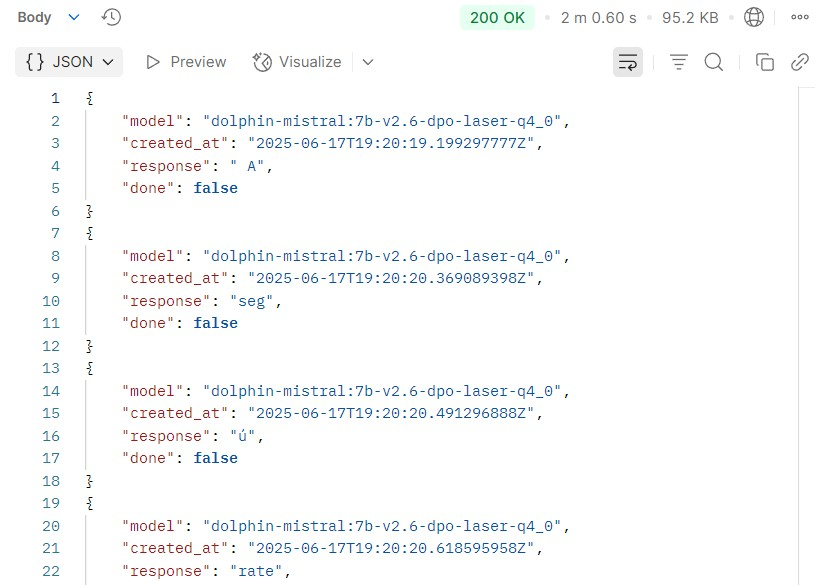
\includegraphics[width=0.8\textwidth]{figs/resUni1.jpg}
  \caption{Resultado de la prueba unitaria sobre el microservicio del modelo LLM}
  \label{fig:resUni1}
\end{figure}

El segundo y último microservicio en ser evaluado es el encargado de generar el modelo 3D a partir de una imagen utilizando el modelo OpenSource de TripoSR. Para efectuar esta prueba, se ha realizado una solicitud POST mediante el software llamado Postman a la dirección del contenedor de TripoSR, específicamente al puerto 5000 y a la terminación de la API \verb|/upload|, donde está alojado el contenedor Docker de este microservicio. La Figura \ref{fig:resUni2} muestra cómo la solicitud retorna un archivo .glb, el cual representa el modelo 3D generado a partir de la imagen de entrada.

% Imagen U2
\begin{figure}[h!tb]
  \centering
  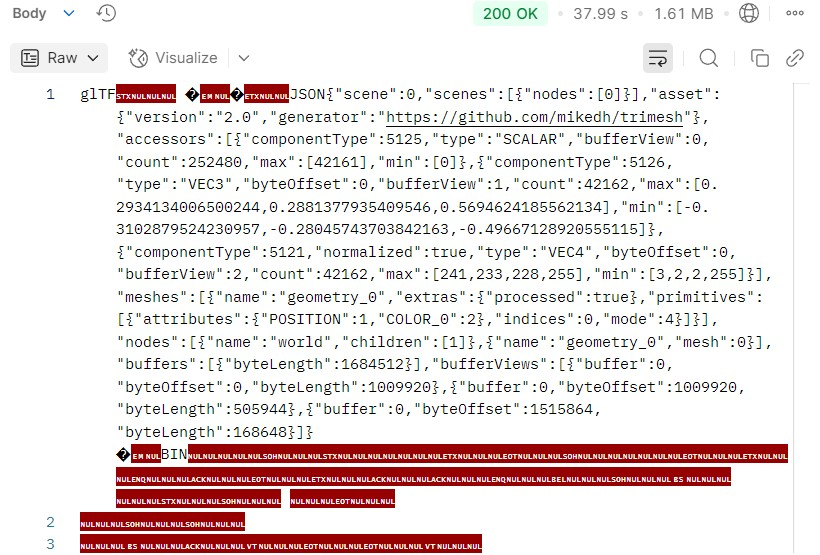
\includegraphics[width=0.8\textwidth]{figs/resUni2.jpg}
  \caption{Resultado de la prueba unitaria sobre el microservicio del modelo TripoSR}
  \label{fig:resUni2}
\end{figure}



\subsection{Pruebas funcionales}
En esta subsección se van a realizar pruebas para comprobar la funcionalidad de cada caso de uso del sistema. La Tabla \ref{tab:pruebasFuncionales}
\begin{table}[h!tb]% Tabla de las pruebas funcionales del sistema
  \centering
  \begin{adjustbox}{max width=0.9\textwidth}
    \begin{tabular}{|p{4cm}|p{4cm}|p{4cm}|p{4cm}|p{2cm}|}
      \hline
      \textbf{Caso de uso}                & \textbf{Prerrequisitos}                                                     & \textbf{Prueba}                                                                                                                                             & \textbf{Resultado esperado}                                                                                                             & \textbf{Figuras}                                   \\ \hline

      CU1:Generar Código Python           & Se debe escribir un prompt de entrada en el Add-on.                         & Realizar la petición de generar código Python.                                                                                                              & Verificar en el terminal del servidor que la solicitud para generar el código Python se lleva a cabo de manera adecuada.                & \ref{fig:cu1cu8}                                   \\ \hline

      CU2:Visualizar Resultado en Blender & Se debe haber obtenido una respuesta del modelo LLM.                        & Ingresar al campo de respuesta del modelo LLM del add-on y proceder a ejecutar el código generado utilizando el botón de ejecución de código.               & Verificar que en el campo de respuesta del modelo LLM está el código y que se ejecuta correctamente.                                    & \ref{fig:cu2_1}, \ref{fig:cu2_2} y \ref{fig:cu2_3} \\ \hline

      CU3:Cargar Imagen                   & Se debe introducir una imagen en el add-on.                                 & Ingresar en la barra de notificaciones de Blender.                                                                                                          & Comprobar en la barra de notificaciones de Blender que se ha cargado correctamente la imagen.                                           & \ref{fig:cu3}                                      \\ \hline

      CU4:Generar Modelo 3D               & Se debe importar una imagen en el add-on.                                   & Realizar la petición de generar el Modelo 3D.                                                                                                               & Verificar en el terminal del servidor que la solicitud para generar el Modelo 3D se lleva a cabo de manera adecuada.                    & \ref{fig:cu4cu9}                                   \\ \hline

      CU5:Cargar modelo 3D en Blender     & Se debe haber obtenido una respuesta del modelo generativo 3D.              & Ingresar al campo de respuesta del modelo generativo 3D del add-on y proceder a cargar el modelo 3D en Blender utilizando el botón de cargar modelo 3D.     & Verificar que en el campo de respuesta del modelo generativo 3D está el modelo 3D y que se carga correctamente en la escena de Blender. & \ref{fig:cu5_1} y \ref{fig:cu5_2}                  \\ \hline

      CU6:Exportar Modelo 3D              & Se debe haber obtenido una respuesta del modelo generativo 3D.              & Ingresar al campo de respuesta del modelo generativo 3D del add-on y proceder a exportar el modelo 3D en Blender utilizando el botón de exportar modelo 3D. & Verificar que se ha exportado correctamente el modelo 3D.                                                                               & \ref{fig:cu6_1} y \ref{fig:cu6_2}                  \\ \hline

      CU7:Deshacer Cambios                & Se debe haber realizado una acción con el add-on en Blender.                & Revertir una acción mediante Ctrl+Z.                                                                                                                        & Verificar en el terminal de Blender que se ha revertido la acción correctamente.                                                        & \ref{fig:cu7}                                      \\ \hline

      CU8:Ejecutar Modelo LLM             & Se debe haber recibido la petición de generar código python en el servidor. & Ingresar al registro de logs de los modelos LLM en el servidor.                                                                                             & Comprobar que se ejecuta el modelo LLM y que devuelve correctamente la respuesta al add-on.                                             & \ref{fig:cu1cu8}                                   \\ \hline

      CU9:Ejecutar Modelo Generativo 3D   & Se debe haber recibido la petición de generar el Modelo 3D en el servidor.  & Ingresar al registro de logs de los modelos generativos 3D en el servidor.                                                                                  & Comprobar que se ejecuta el modelo generativo 3D y que devuelve correctamente la respuesta al add-on.                                   & \ref{fig:cu4cu9}                                   \\ \hline
    \end{tabular}
  \end{adjustbox}
  \caption{Tabla con las pruebas funcionales del sistema}
  \label{tab:pruebasFuncionales}
\end{table}
muestra los casos de uso junto con los requisitos previos, los pasos requeridos para llevar a cabo las pruebas y los resultados que se anticipan.
A continuación, se procederá a realizar todas las pruebas mencionadas antes, incluyendo capturas de pantalla o listados de logs que evidencien que los resultados anticipados se cumplen. Estos resultados se registran en el Apéndice \ref{sec:puntoB1} para cada caso de uso dentro del sistema.

% \begin{itemize}
%     \item \textbf{CU1 y CU8:} La Figura \ref{fig:cu1cu8} muestra los resultados alcanzados.

%     \item \textbf{CU2:} La Figura \ref{fig:cu2_1}, \ref{fig:cu2_2} y \ref{fig:cu2_3} muestra los resultados alcanzados.

%     \item \textbf{CU3:} La Figura \ref{fig:cu3} muestra los resultados alcanzados.

%     \item \textbf{CU4 y CU9:} La Figura \ref{fig:cu4cu9} muestra los resultados alcanzados.

%     \item \textbf{CU5:} La Figura \ref{fig:cu5_1} y \ref{fig:cu5_2} muestra los resultados alcanzados.

%     \item \textbf{CU6:} La Figura \ref{fig:cu6_1} y \ref{fig:cu6_2} muestra los resultados alcanzados.

%     \item \textbf{CU7:} La Figura \ref{fig:cu7} muestra los resultados alcanzados.
% \end{itemize}


\subsection{Pruebas de rendimiento}
Las pruebas de rendimiento descritas en esta subsección tienen como finalidad evaluar la capacidad del sistema para mantener un funcionamiento estable bajo condiciones de alta demanda concurrente. El objetivo es obtener métricas clave como el tiempo medio de respuesta y el comportamiento del sistema ante situaciones de estrés. Para su ejecución, se ha diseñado un conjunto de experimentos consistentes en el envío de solicitudes simultáneas a los modelos de IA integrados (modelo LLM y modelo generativo 3D), simulando mediante el software de Postman las peticiones de los múltiples dispositivos. La carga generada se incrementa progresivamente, comenzando con una única petición dirigida a cada modelo y alcanzando hasta cuatro peticiones simultáneas por tipo de modelo. Este límite ha sido definido teniendo en cuenta las restricciones del entorno de pruebas, que se ejecuta sobre un hardware limitado y con recursos computacionales reducidos, donde el servidor ha sido desplegado con dos instancias por modelo de \gls{ia}, por lo que cuatro solicitudes concurrentes equivalen a una carga del 200\%, superando intencionadamente la capacidad nominal para observar el comportamiento bajo saturación. Dado que los dispositivos desde los cuales se emiten las peticiones son externos a la red local del servidor, ha sido necesario utilizar un mecanismo de acceso remoto a los servicios expuestos localmente. Para ello, se ha empleado la herramienta Postman, que permite la creación personalizada de peticiones, la automatización de las mismas y brinda estadísticas de cada petición y respuesta. Por otro lado, para medir el consumo y estrés del sistema en las diferentes pruebas se ha empleado la herramienta de htop en la máquina virtual del servidor, que permite visualizar el consumo de todos los núcleos de la CPU, de la memoria RAM, de la memoria Swap y visualizar el consumo de cada tarea.

Tras la ejecución de las pruebas de rendimiento, se ha observado un comportamiento progresivo en el consumo de recursos del sistema asociado al modelo de lenguaje LLM. Tal como se muestra en la Figura \ref{fig:resRend1LLM}, correspondiente a una única petición simultánea, el sistema presenta un uso medio de CPU del 74,7 \% y un consumo de memoria del 25,6 \%, sin llegar a utilizar ningún núcleo de procesamiento de forma completa y manteniéndose recursos disponibles para otras operaciones concurrentes.
% % Imagen R1
%   \begin{figure}[h!tb]
%     \centering
%     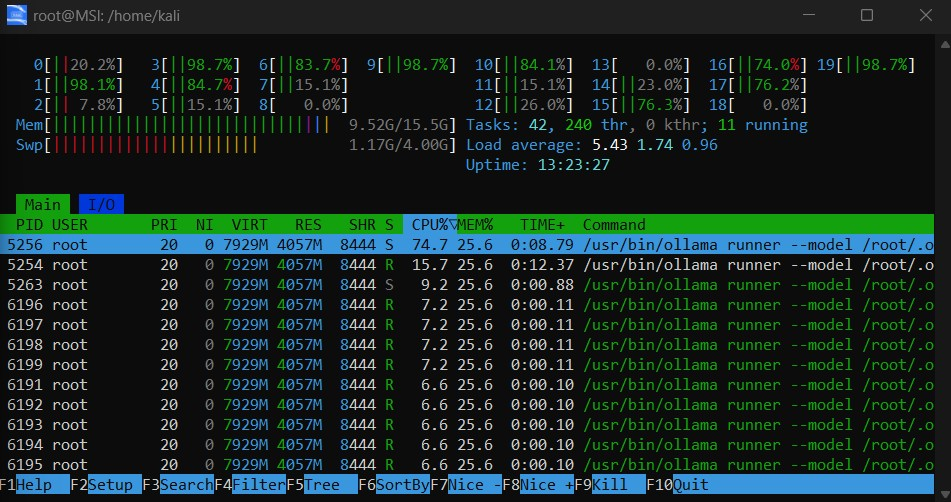
\includegraphics[width=0.8\textwidth]{figs/LLM1.jpg}
%     \caption{Resultado de la prueba de rendimiento con 1 petición sobre el microservicio del modelo LLM}
%     \label{fig:resRend1LLM}
%   \end{figure}

No obstante, al incrementar la carga con múltiples peticiones simultáneas, se evidencia un aumento significativo en la utilización de la CPU, como se ilustra en las Figuras \ref{fig:resRend2LLM} y \ref{fig:resRend3LLM}, alcanzando en el caso de cuatro solicitudes concurrentes un valor ligeramente superior al 100 \% de 100,5 \% de uso de CPU, mientras que el uso de memoria permanece estable en torno al 25,4 \%, esto último se puede observar en la Figura \ref{fig:resRend4LLM}.

% % Imagen R2
%   \begin{figure}[h!tb]
%     \centering
%     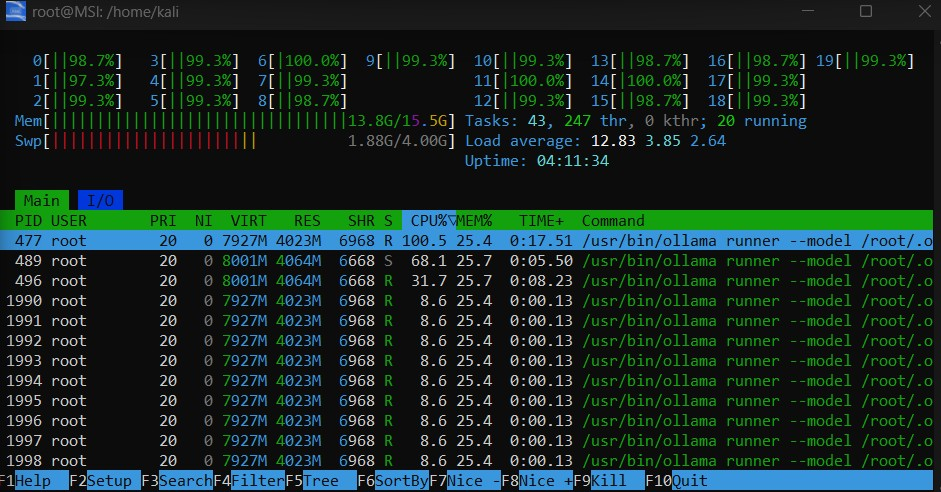
\includegraphics[width=0.8\textwidth]{figs/LLM4.jpg}
%     \caption{Resultado de la prueba de rendimiento con 4 petición sobre el microservicio del modelo LLM}
%     \label{fig:resRend4LLM}
%   \end{figure}

Este incremento en la demanda de recursos impacta directamente en la latencia de la última solicitud procesada, la cual experimenta un retraso derivado de la espera por disponibilidad de recursos computacionales y contenedores con el modelo LLM disponibles. Cabe destacar que, de acuerdo con los resultados presentados en la Tabla \ref{tab:pruebasRendimiento}, el modelo LLM presenta tiempos de respuesta superiores respecto al modelo generativo 3D, siendo el componente más lento en condiciones de carga equivalente. Esta diferencia operativa motivó la implementación del mecanismo de streaming en las respuestas del modelo LLM, permitiendo que, a pesar de una latencia total mayor, las primeras porciones de salida sean entregadas al usuario antes que en el caso del modelo generativo 3D, optimizando así la percepción de fluidez en la interacción.

% Tabla de las pruebas de usabilidad 2
\begin{table}[h!tb]
  \centering
  \begin{adjustbox}{max width=\textwidth}
    \begin{tabular}{|>{\centering\arraybackslash}p{4cm}|>{\centering\arraybackslash}p{4cm}|>{\centering\arraybackslash}p{4cm}|>{\centering\arraybackslash}p{4cm}|>{\centering\arraybackslash}p{4cm}|}
      \hline
      \textbf{Servicio}   & \textbf{Tiempo máximo (1 petición)} & \textbf{Tiempo máximo (2 petición)} & \textbf{Tiempo máximo (3 petición)} & \textbf{Tiempo máximo (4 petición)} \\ \hline

      Modelo LLM (Ollama) & 1 m 36.90 s                         & 3 m 0.30 s                          & 3 m 44.34 s                         & 3 m 50.12 s                         \\ \hline

      Modelo 3D (TripoSR) & 40.73 s                             & 1 m 23.34 s                         & 1 m 51.30 s                         & 2 m 30.12 s                         \\ \hline
    \end{tabular}
  \end{adjustbox}
  \caption{Tabla de tiempo de espera máxima por petición asociada a cada modelo de IA}
  \label{tab:pruebasRendimiento}
\end{table}


La Figura \ref{fig:resRend13D} presenta los resultados del análisis de rendimiento correspondiente a una única petición simultánea dirigida al modelo generativo 3D.
% % Imagen R3
%   \begin{figure}[h!tb]
%     \centering
%     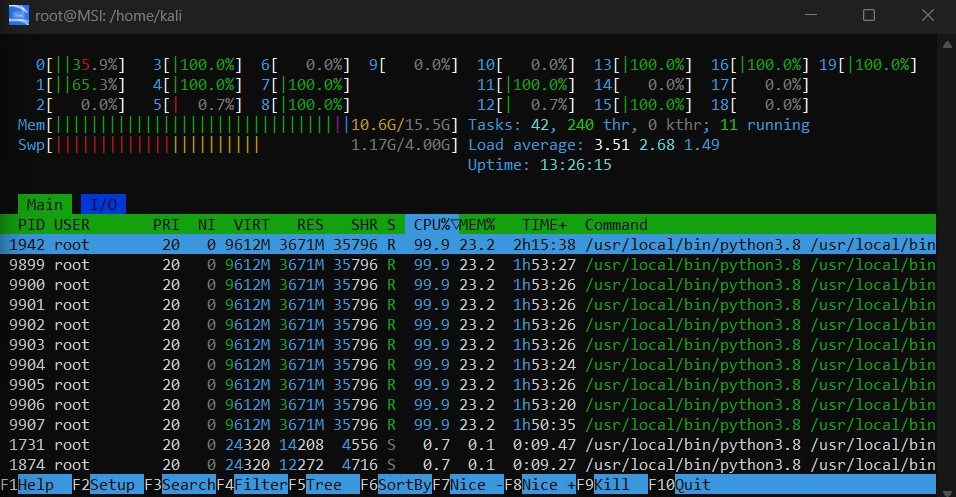
\includegraphics[width=0.8\textwidth]{figs/3D1.jpg}
%     \caption{Resultado de la prueba de rendimiento con 1 petición sobre el microservicio del modelo 3D TripoSR}
%     \label{fig:resRend13D}
%   \end{figure}
En ella se observa una utilización media de CPU del 99,9 \% y un consumo de memoria del 23,2 \%, haciendo uso intensivo de la mayoría de núcleos disponibles en el procesador. A medida que se incrementa la carga del sistema mediante múltiples solicitudes concurrentes, se constata un aumento aún más acusado en el uso de CPU en comparación con el modelo LLM, tal como se evidencia en las Figuras \ref{fig:resRend23D} y \ref{fig:resRend33D}. En el escenario con cuatro peticiones simultáneas de la Figura \ref{fig:resRend43D}, la carga computacional alcanza un valor de 100,7 \%, lo que sugiere una saturación prácticamente total de los recursos de procesamiento, mientras que la memoria RAM se mantiene relativamente estable, con un promedio de uso en torno al 24,7 \%. Este aumento en la demanda de recursos afecta directamente a la latencia observada en la última petición en ser atendida, debido a la necesidad de esperar la liberación de núcleos o la disponibilidad de instancias del contenedor del modelo 3D para poder procesarla. Es importante señalar que, según los datos recopilados, a partir de dos solicitudes concurrentes ya se produce una ocupación completa de los núcleos del procesador, lo que pone de manifiesto el elevado coste computacional asociado a la ejecución del modelo TripoSR en un hardware limitado.

% % Imagen R4
%   \begin{figure}[h!tb]
%     \centering
%     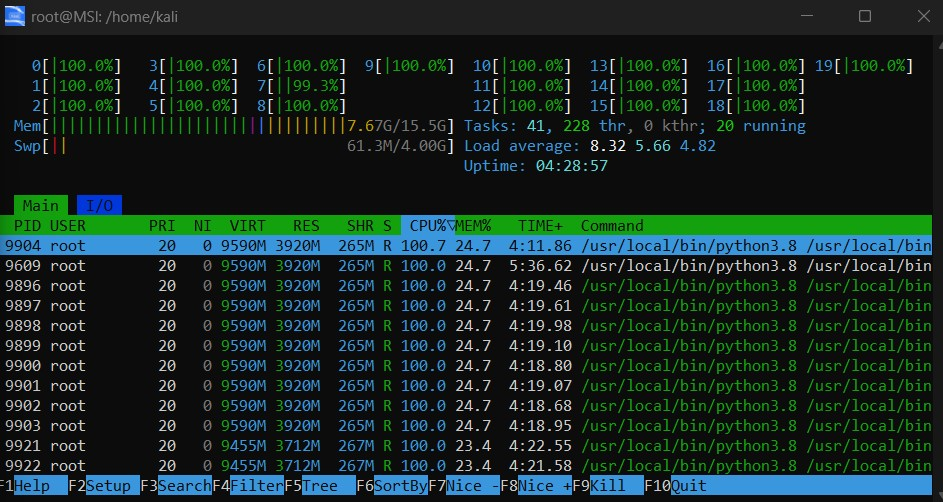
\includegraphics[width=0.8\textwidth]{figs/3D4.jpg}
%     \caption{Resultado de la prueba de rendimiento con 4 petición sobre el microservicio del modelo 3D TripoSR}
%     \label{fig:resRend43D}
%   \end{figure}



\subsection{Pruebas de usabilidad}
En esta subsección se va a evaluar la calidad percibida en términos de facilidad de uso del complemento desarrollado para Blender, se ha adoptado como instrumento de análisis el método \gls{sus}. Este procedimiento es ampliamente reconocido en el ámbito de la evaluación de interfaces de usuario por su simplicidad, fiabilidad y aplicabilidad transversal a distintos tipos de sistemas interactivos. El cuestionario está compuesto por diez afirmaciones (ver Tabla \ref{tab:preguntasSUS}) que deben ser valoradas por los usuarios empleando una escala de tipo Likert de cinco puntos, donde 1 corresponde a “totalmente en desacuerdo” y 5 a “totalmente de acuerdo”. Las afirmaciones se estructuran alternando enunciados de formulación positiva y negativa, lo que permite mitigar sesgos de respuesta y obtener una valoración más equilibrada de la experiencia de uso. El instrumento está diseñado de forma genérica, permitiendo su aplicación en una amplia variedad de entornos tecnológicos y facilitando la comparación entre soluciones de distinta naturaleza. El cálculo de la puntuación total se realiza mediante una transformación lineal, en el caso de los ítems con redacción positiva (ítems impares), se resta 1 al valor proporcionado por el usuario/a, para los ítems negativos (ítems pares), se resta la puntuación a 5. La suma de los valores transformados (en un rango de 0 a 40) se multiplica por un factor de 2.5, obteniéndose así una puntuación final normalizada en una escala de 0 a 100. Según los estándares investigados, una puntuación cercana a 68 se considera indicativa de una usabilidad media, valores superiores a 80 reflejan una percepción de alta usabilidad, mientras que resultados por debajo de 50 revelan deficiencias significativas en la experiencia de uso. En el marco del presente trabajo, este método ha sido aplicado a una muestra de usuarios que interactuaron con el add-on diseñado para Blender. La finalidad ha sido obtener una valoración cuantitativa objetiva sobre la facilidad de uso, el grado de integración funcional y la curva de aprendizaje percibida del sistema, con el fin de identificar posibles áreas de mejora en futuras iteraciones del desarrollo.\\

% Tabla de las pruebas de usabilidad 2
\begin{table}[h!tb]
  \centering
  \begin{adjustbox}{max width=\textwidth}
    \begin{tabular}{|>{\centering\arraybackslash}p{2cm}|>{\centering\arraybackslash}p{10cm}|}
      \hline
      \textbf{Número} & \textbf{Pregunta}                                                \\ \hline

      Q1              & ¿Me gustaría usarlo con frecuencia?                              \\ \hline

      Q2              & ¿Lo encontré innecesariamente complejo?                          \\ \hline

      Q3              & ¿Lo encontré fácil de usar?                                      \\ \hline

      Q4              & ¿Pensé que haría falta mucha ayuda para usarlo?                  \\ \hline

      Q5              & ¿Las funciones estaban bien integradas?                          \\ \hline

      Q6              & ¿Encontré demasiada inconsistencia en el sistema?                \\ \hline

      Q7              & ¿Imagino que la mayoría aprendería a usarlo muy rápidamente?     \\ \hline

      Q8              & ¿Encontré el sistema difícil de usar?                            \\ \hline

      Q9              & ¿Me sentí muy confiado usándolo?                                 \\ \hline

      Q10             & ¿Necesité aprender muchas cosas antes de poder funcionar con él? \\ \hline
    \end{tabular}
  \end{adjustbox}
  \caption{Tabla de preguntas del método SUS}
  \label{tab:preguntasSUS}
\end{table}

% \textbf{Componentes del SUS:}
% \begin{enumerate}
%     \item Me gustaría usarlo con frecuencia.
%     \item Lo encontré innecesariamente complejo.
%     \item Lo encontré fácil de usar.
%     \item Pensé que haría falta mucha ayuda para usarlo.
%     \item Las funciones estaban bien integradas.
%     \item Encontré demasiada inconsistencia en el sistema.
%     \item Imagino que la mayoría aprendería a usarlo muy rápidamente.
%     \item Encontré el sistema difícil de usar.
%     \item Me sentí muy confiado usándolo.
%     \item Necesité aprender muchas cosas antes de poder funcionar con él.
% \end{enumerate}

El análisis estadístico de las puntuaciones obtenidas mediante la aplicación del cuestionario SUS en las Tablas \ref{tab:pruebasUsabilidad1} y \ref{tab:pruebasUsabilidad2} revela una alta valoración general de la usabilidad del sistema, con una media aritmética de 89.3 sobre 100 y una desviación estándar de 2.9. Estos resultados reflejan una percepción homogénea por parte de los usuarios, respaldada por un coeficiente de variación del 3.25 \%, lo que indica una baja dispersión relativa respecto a la media. El rango de puntuaciones registrado, comprendido entre 85.0 y 92.5, refuerza la estabilidad de las evaluaciones y la consistencia en la experiencia de uso reportada. Cabe destacar que la totalidad de las respuestas se sitúan por encima del umbral de 80.3 que define una experiencia bastante buena en términos de usabilidad.

% Tabla de las pruebas de usabilidad 1
\begin{table}[h!tb]
  \centering
  \begin{adjustbox}{max width=\textwidth}
    \begin{tabular}{|>{\centering\arraybackslash}p{3cm}|>{\centering\arraybackslash}p{1cm}|>{\centering\arraybackslash}p{1cm}|>{\centering\arraybackslash}p{1cm}|>{\centering\arraybackslash}p{1cm}|>{\centering\arraybackslash}p{1cm}|>{\centering\arraybackslash}p{1cm}|>{\centering\arraybackslash}p{1cm}|>{\centering\arraybackslash}p{1cm}|>{\centering\arraybackslash}p{1cm}|>{\centering\arraybackslash}p{1cm}|>{\centering\arraybackslash}p{2cm}|}
      \hline
      \textbf{Participante} & \textbf{Q1} & \textbf{Q2} & \textbf{Q3} & \textbf{Q4} & \textbf{Q5} & \textbf{Q6} & \textbf{Q7} & \textbf{Q8} & \textbf{Q9} & \textbf{Q10} & \textbf{SUS (0-100)} \\ \hline

      1                     & 4           & 5           & 4           & 5           & 5           & 4           & 5           & 4           & 5           & 5            & 92.5                 \\ \hline

      2                     & 5           & 4           & 5           & 4           & 4           & 5           & 4           & 5           & 4           & 4            & 85.0                 \\ \hline

      3                     & 4           & 5           & 4           & 5           & 5           & 4           & 5           & 4           & 5           & 4            & 90.0                 \\ \hline

      4                     & 5           & 4           & 5           & 4           & 4           & 5           & 4           & 5           & 5           & 5            & 87.5                 \\ \hline

      5                     & 4           & 5           & 4           & 5           & 5           & 4           & 5           & 4           & 4           & 5            & 90.0                 \\ \hline

      6                     & 5           & 4           & 5           & 4           & 5           & 5           & 4           & 5           & 5           & 4            & 87.5                 \\ \hline

      7                     & 4           & 5           & 4           & 5           & 4           & 5           & 5           & 4           & 5           & 5            & 92.5                 \\ \hline
    \end{tabular}
  \end{adjustbox}
  \caption{Tabla de puntuaciones SUS para las pruebas de usabilidad}
  \label{tab:pruebasUsabilidad1}
\end{table}

% Tabla de las pruebas de usabilidad 2
\begin{table}[h!tb]
  \centering
  \begin{adjustbox}{max width=\textwidth}
    \begin{tabular}{|>{\centering\arraybackslash}p{4cm}|>{\centering\arraybackslash}p{4cm}|}
      \hline
      \textbf{Métrica}    & \textbf{Valor} \\ \hline

      Promedio SUS        & 89.3           \\ \hline

      Mínimo SUS          & 85.0           \\ \hline

      Máximo SUS          & 92.5           \\ \hline

      Desviación Estándar & 2.9            \\ \hline
    \end{tabular}
  \end{adjustbox}
  \caption{Tabla de los valores promedio de las puntuaciones SUS correspondientes a las pruebas de usabilidad}
  \label{tab:pruebasUsabilidad2}
\end{table}



\subsection{Pruebas de seguridad}
Esta última subsección tiene como propósito analizar el nivel de seguridad del sistema implementado, identificando posibles vulnerabilidades mediante técnicas de escaneo automatizado. Para ello, se ha utilizado la herramienta \gls{zap} \cite{ZAPHomepage}, desarrollada por OWASP y ampliamente reconocida en el ámbito de la ciberseguridad, que permite realizar análisis activos sobre aplicaciones web evaluando el comportamiento de endpoints y URLs frente a múltiples vectores de ataque. En el contexto de este proyecto, se ha empleado ZAP para someter a análisis los dos servicios expuestos del servidor de inteligencia artificial, el modelo de lenguaje LLM, accesible mediante el endpoint \verb|http://127.0.0.1:11434/api/generate| y el modelo generativo 3D, ubicado en \verb|http://127.0.0.1:5000/upload|.\\

En el primer caso, correspondiente al modelo LLM, los resultados del escaneo activo mostrados en la Figura \ref{fig:secLLM}
% Imagen S1
\begin{figure}[h!tb]
  \centering
  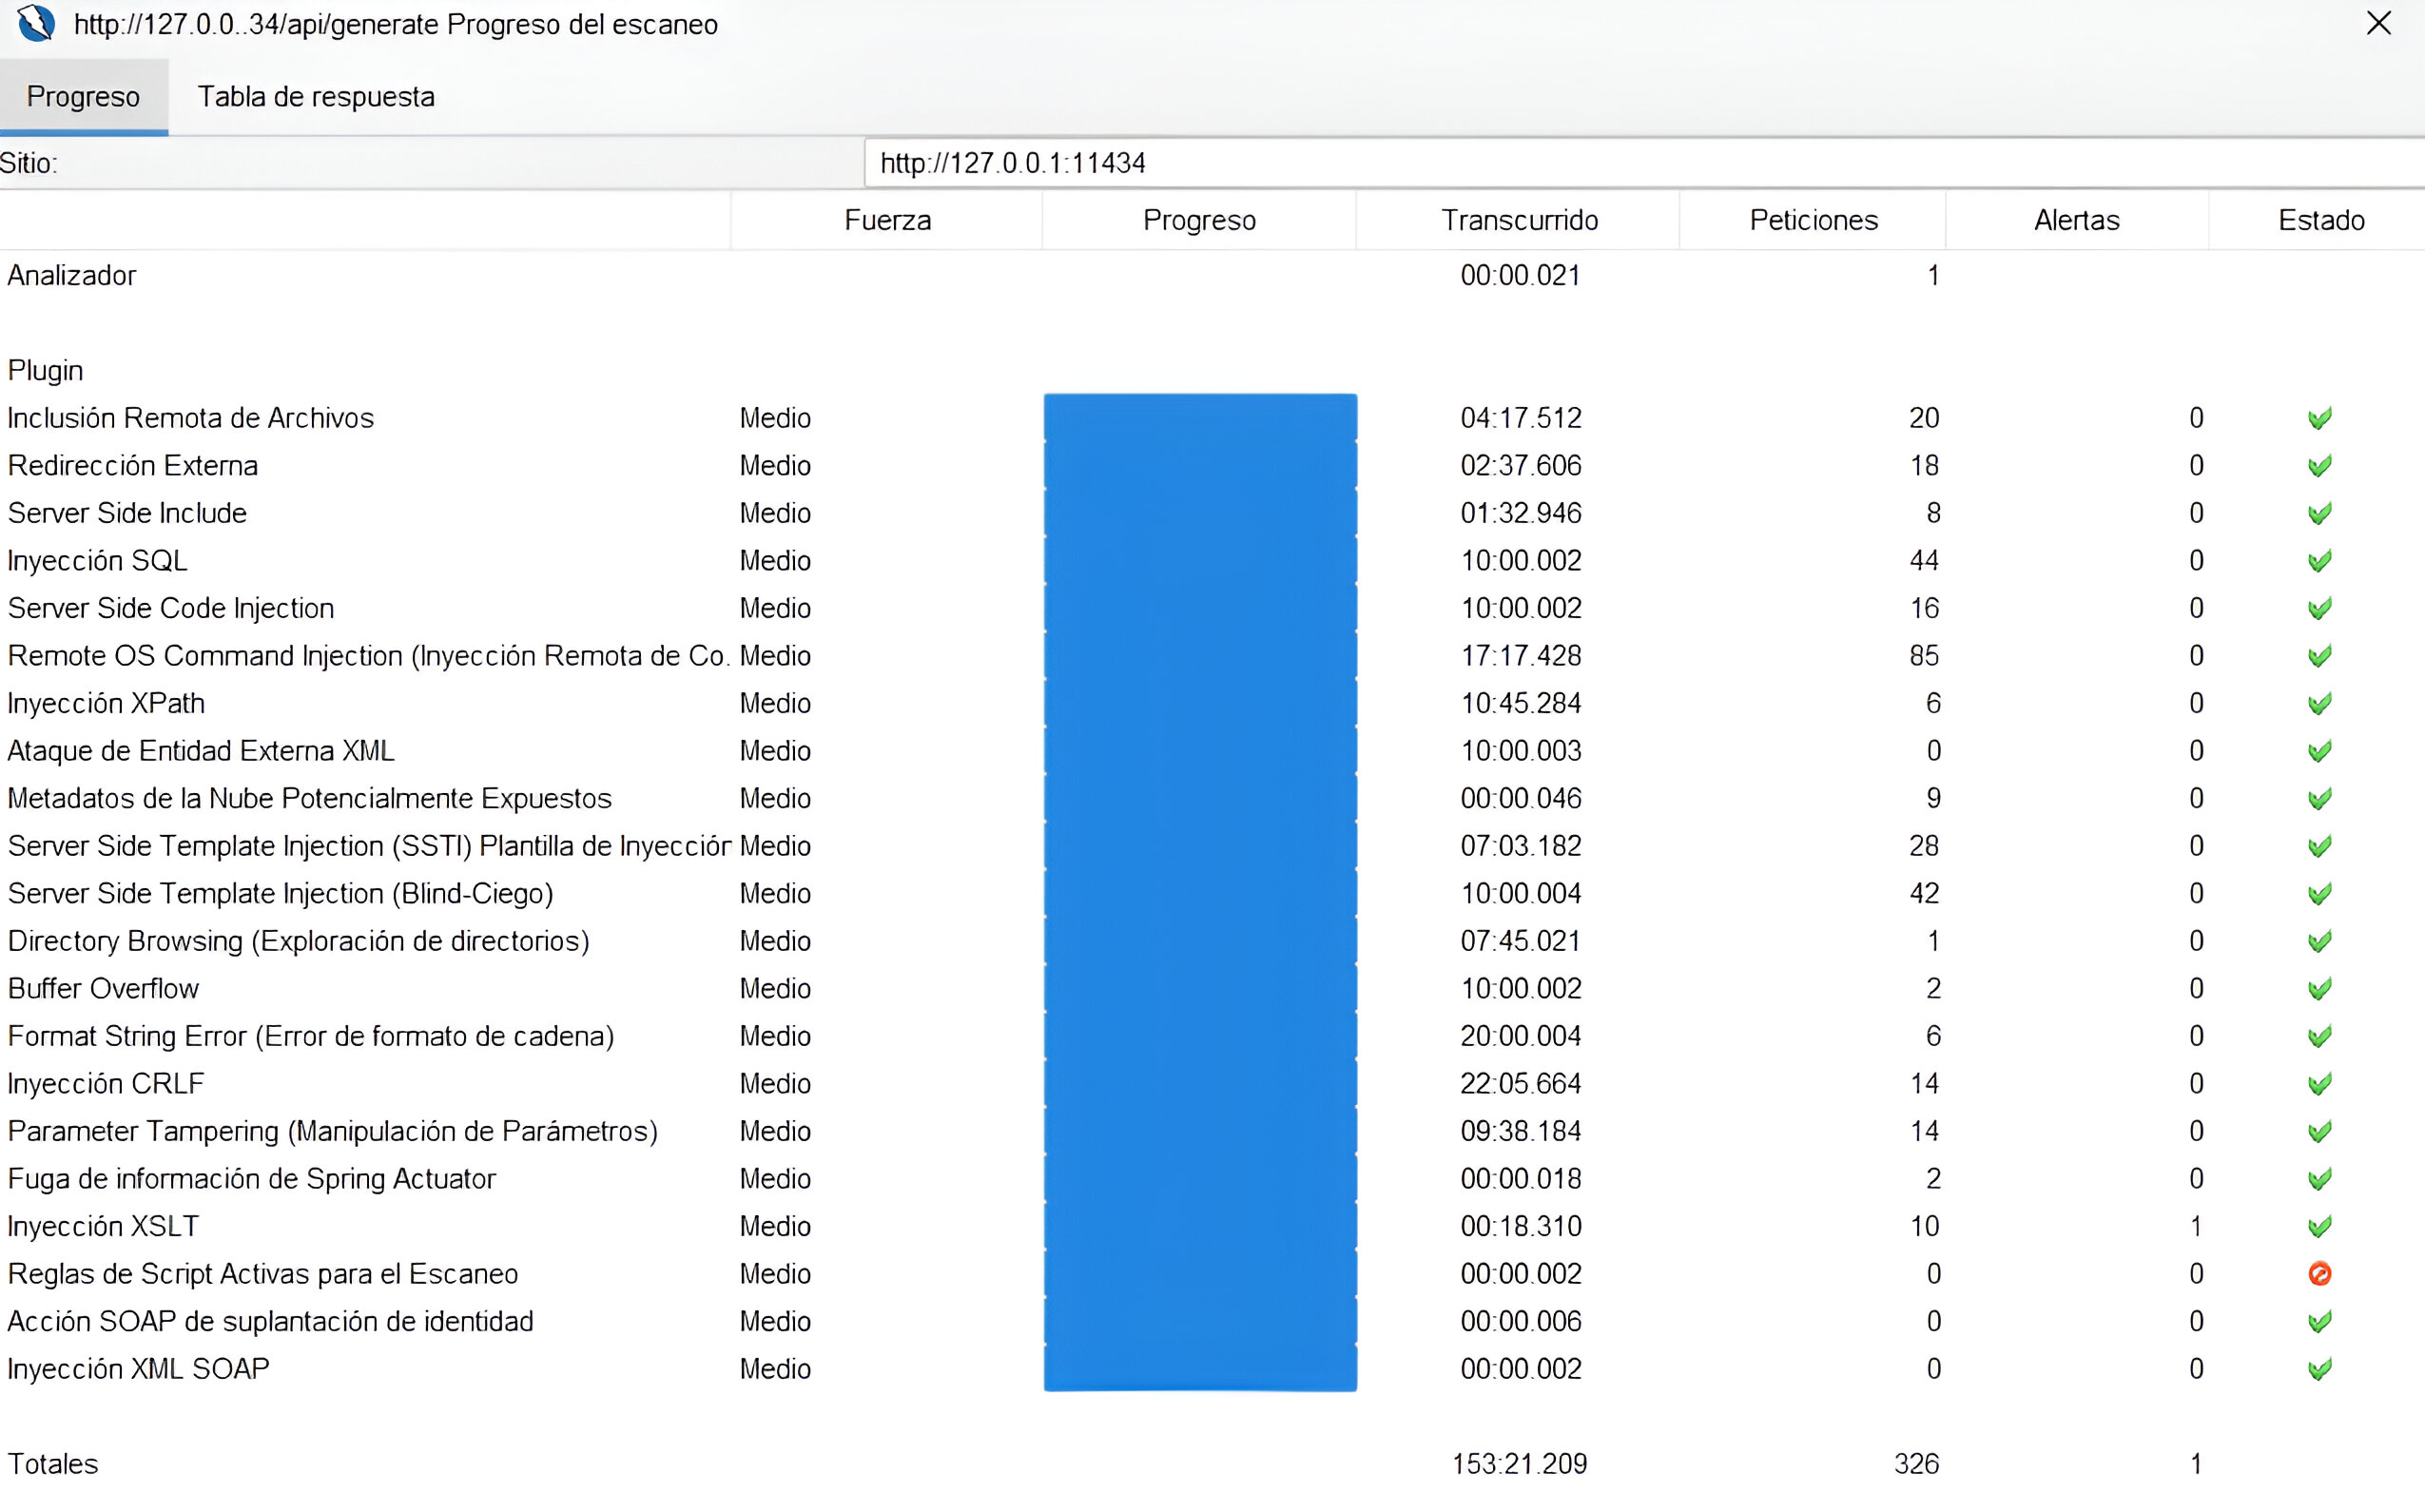
\includegraphics[width=1.0\textwidth]{figs/secLLM.jpg}
  \caption{Resultado de la prueba de seguridad sobre el endpoint del modelo LLM del servidor}
  \label{fig:secLLM}
\end{figure}
indican que la mayoría de las pruebas de seguridad fueron superadas satisfactoriamente, con excepción de las reglas asociadas a la ejecución de scripts, que no se encontraban configuradas.
No obstante, se identificó una alerta de severidad media relacionada con una posible inyección XSLT, asociada al CWE-91. El test realizado por ZAP incluyó el uso del payload \verb|xsl:value-of select="system-property('xsl vendor')"| y, como respuesta, el servidor devolvió la cadena \verb|"Microsoft"|, lo cual fue interpretado como un indicio de vulnerabilidad, tal como se muestra en la Figura \ref{fig:secVuln1}.

% Imagen S3
\begin{figure}[h!tb]
  \centering
  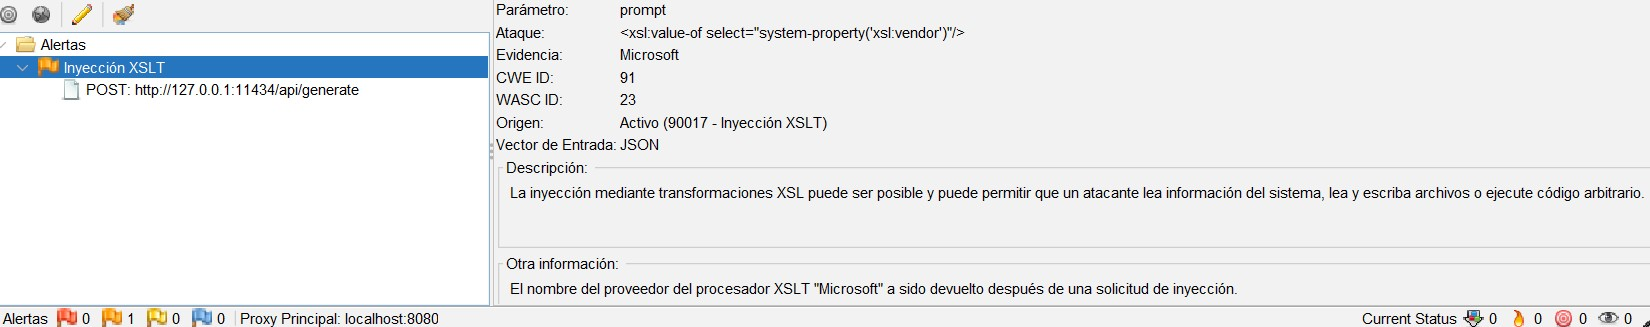
\includegraphics[width=1.0\textwidth]{figs/secVuln1.jpg}
  \caption{Vulnerabilidades obtenidas en el modelo LLM}
  \label{fig:secVuln1}
\end{figure}

Sin embargo, tras un análisis detallado del flujo de salida, representado en la Figura \ref{fig:secVuln2}, se comprobó que dicha respuesta no era resultado de una ejecución arbitraria, sino que coincidía con un fragmento generado por el propio modelo \gls{llm} en modo streaming, siendo “Microsoft” simplemente parte del contenido textual generado por el modelo en respuesta al prompt.
Esta interpretación se refuerza por el hecho de que el sistema operativo subyacente sobre el que se ejecuta el servidor es Linux, descartando así la hipótesis de una fuga real de información a través del subsistema XSLT.

% Imagen S4
\begin{figure}[h!tb]
  \centering
  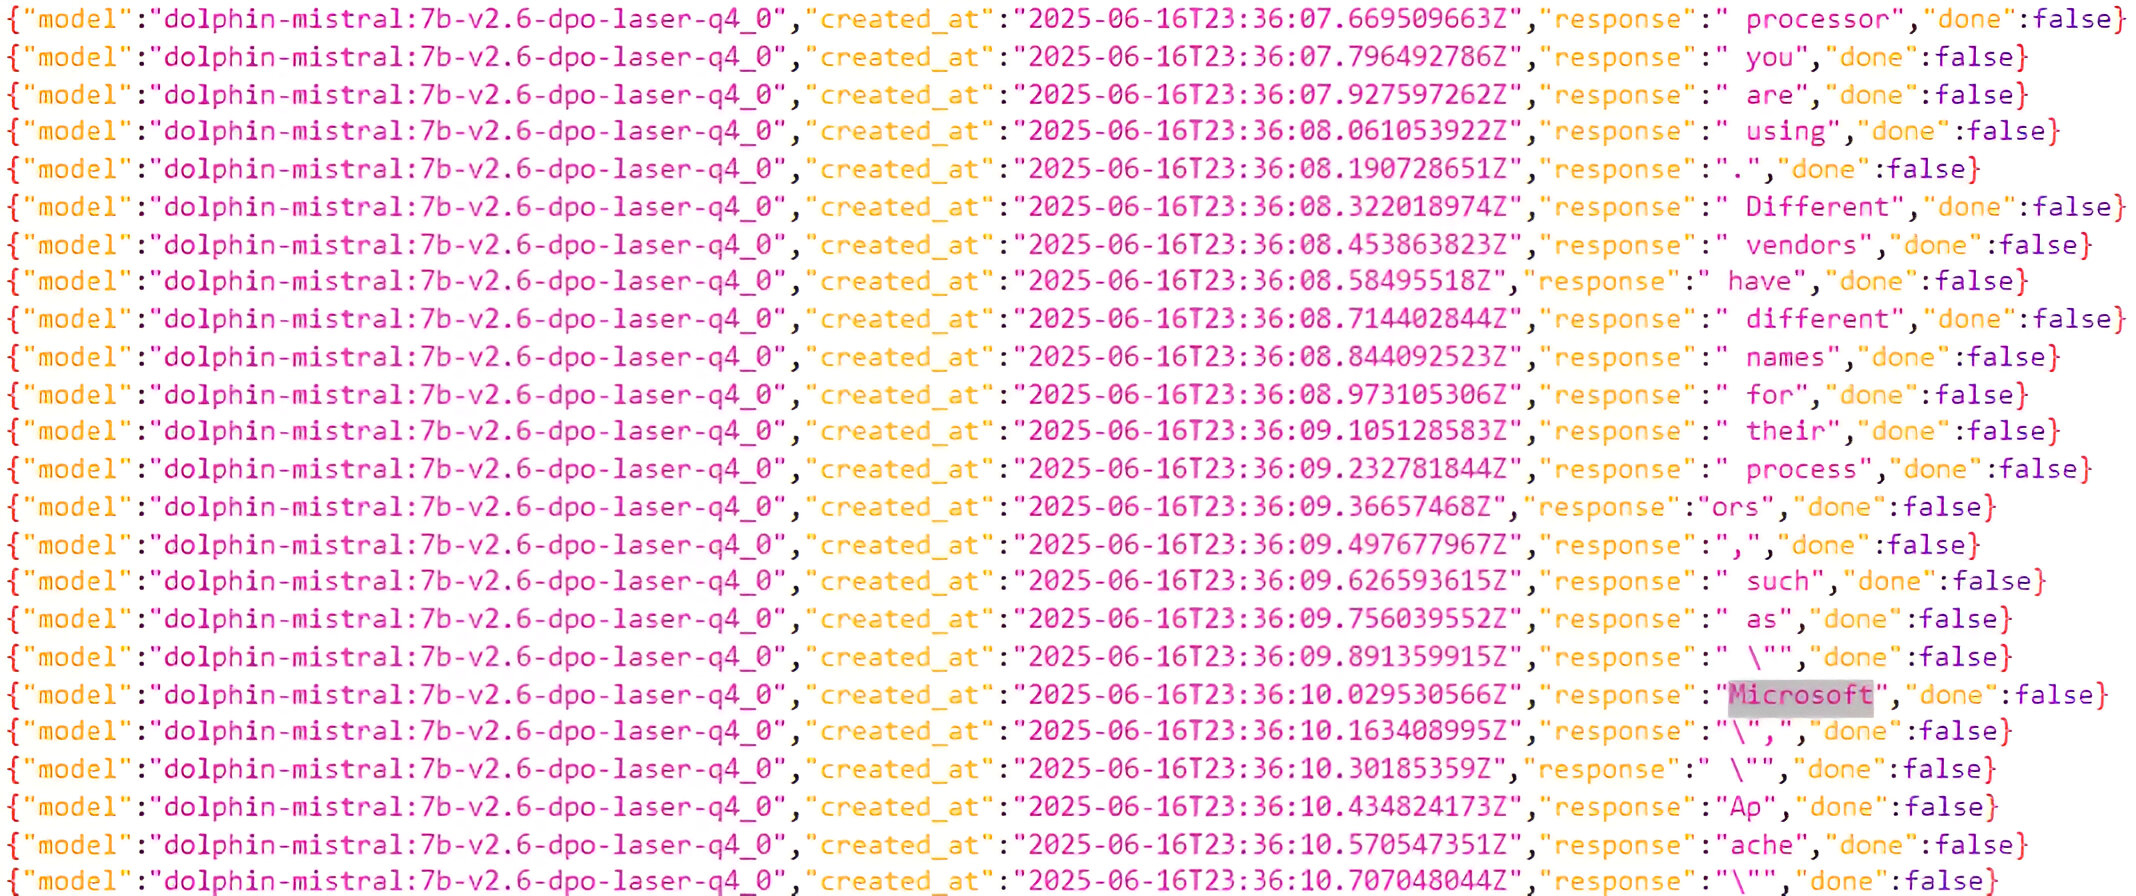
\includegraphics[width=1.0\textwidth]{figs/secVuln2.jpg}
  \caption{Detalles de la vulnerabilidad encontrada en el modelo LLM}
  \label{fig:secVuln2}
\end{figure}

En el segundo caso, correspondiente al endpoint del modelo 3D, el análisis de seguridad, consulte la Figura \ref{fig:sec3D}, mostró resultados similares y reportó también una alerta de alta severidad relacionada con una posible inyección remota de comandos (CWE-78).
% Imagen S2
\begin{figure}[h!tb]
  \centering
  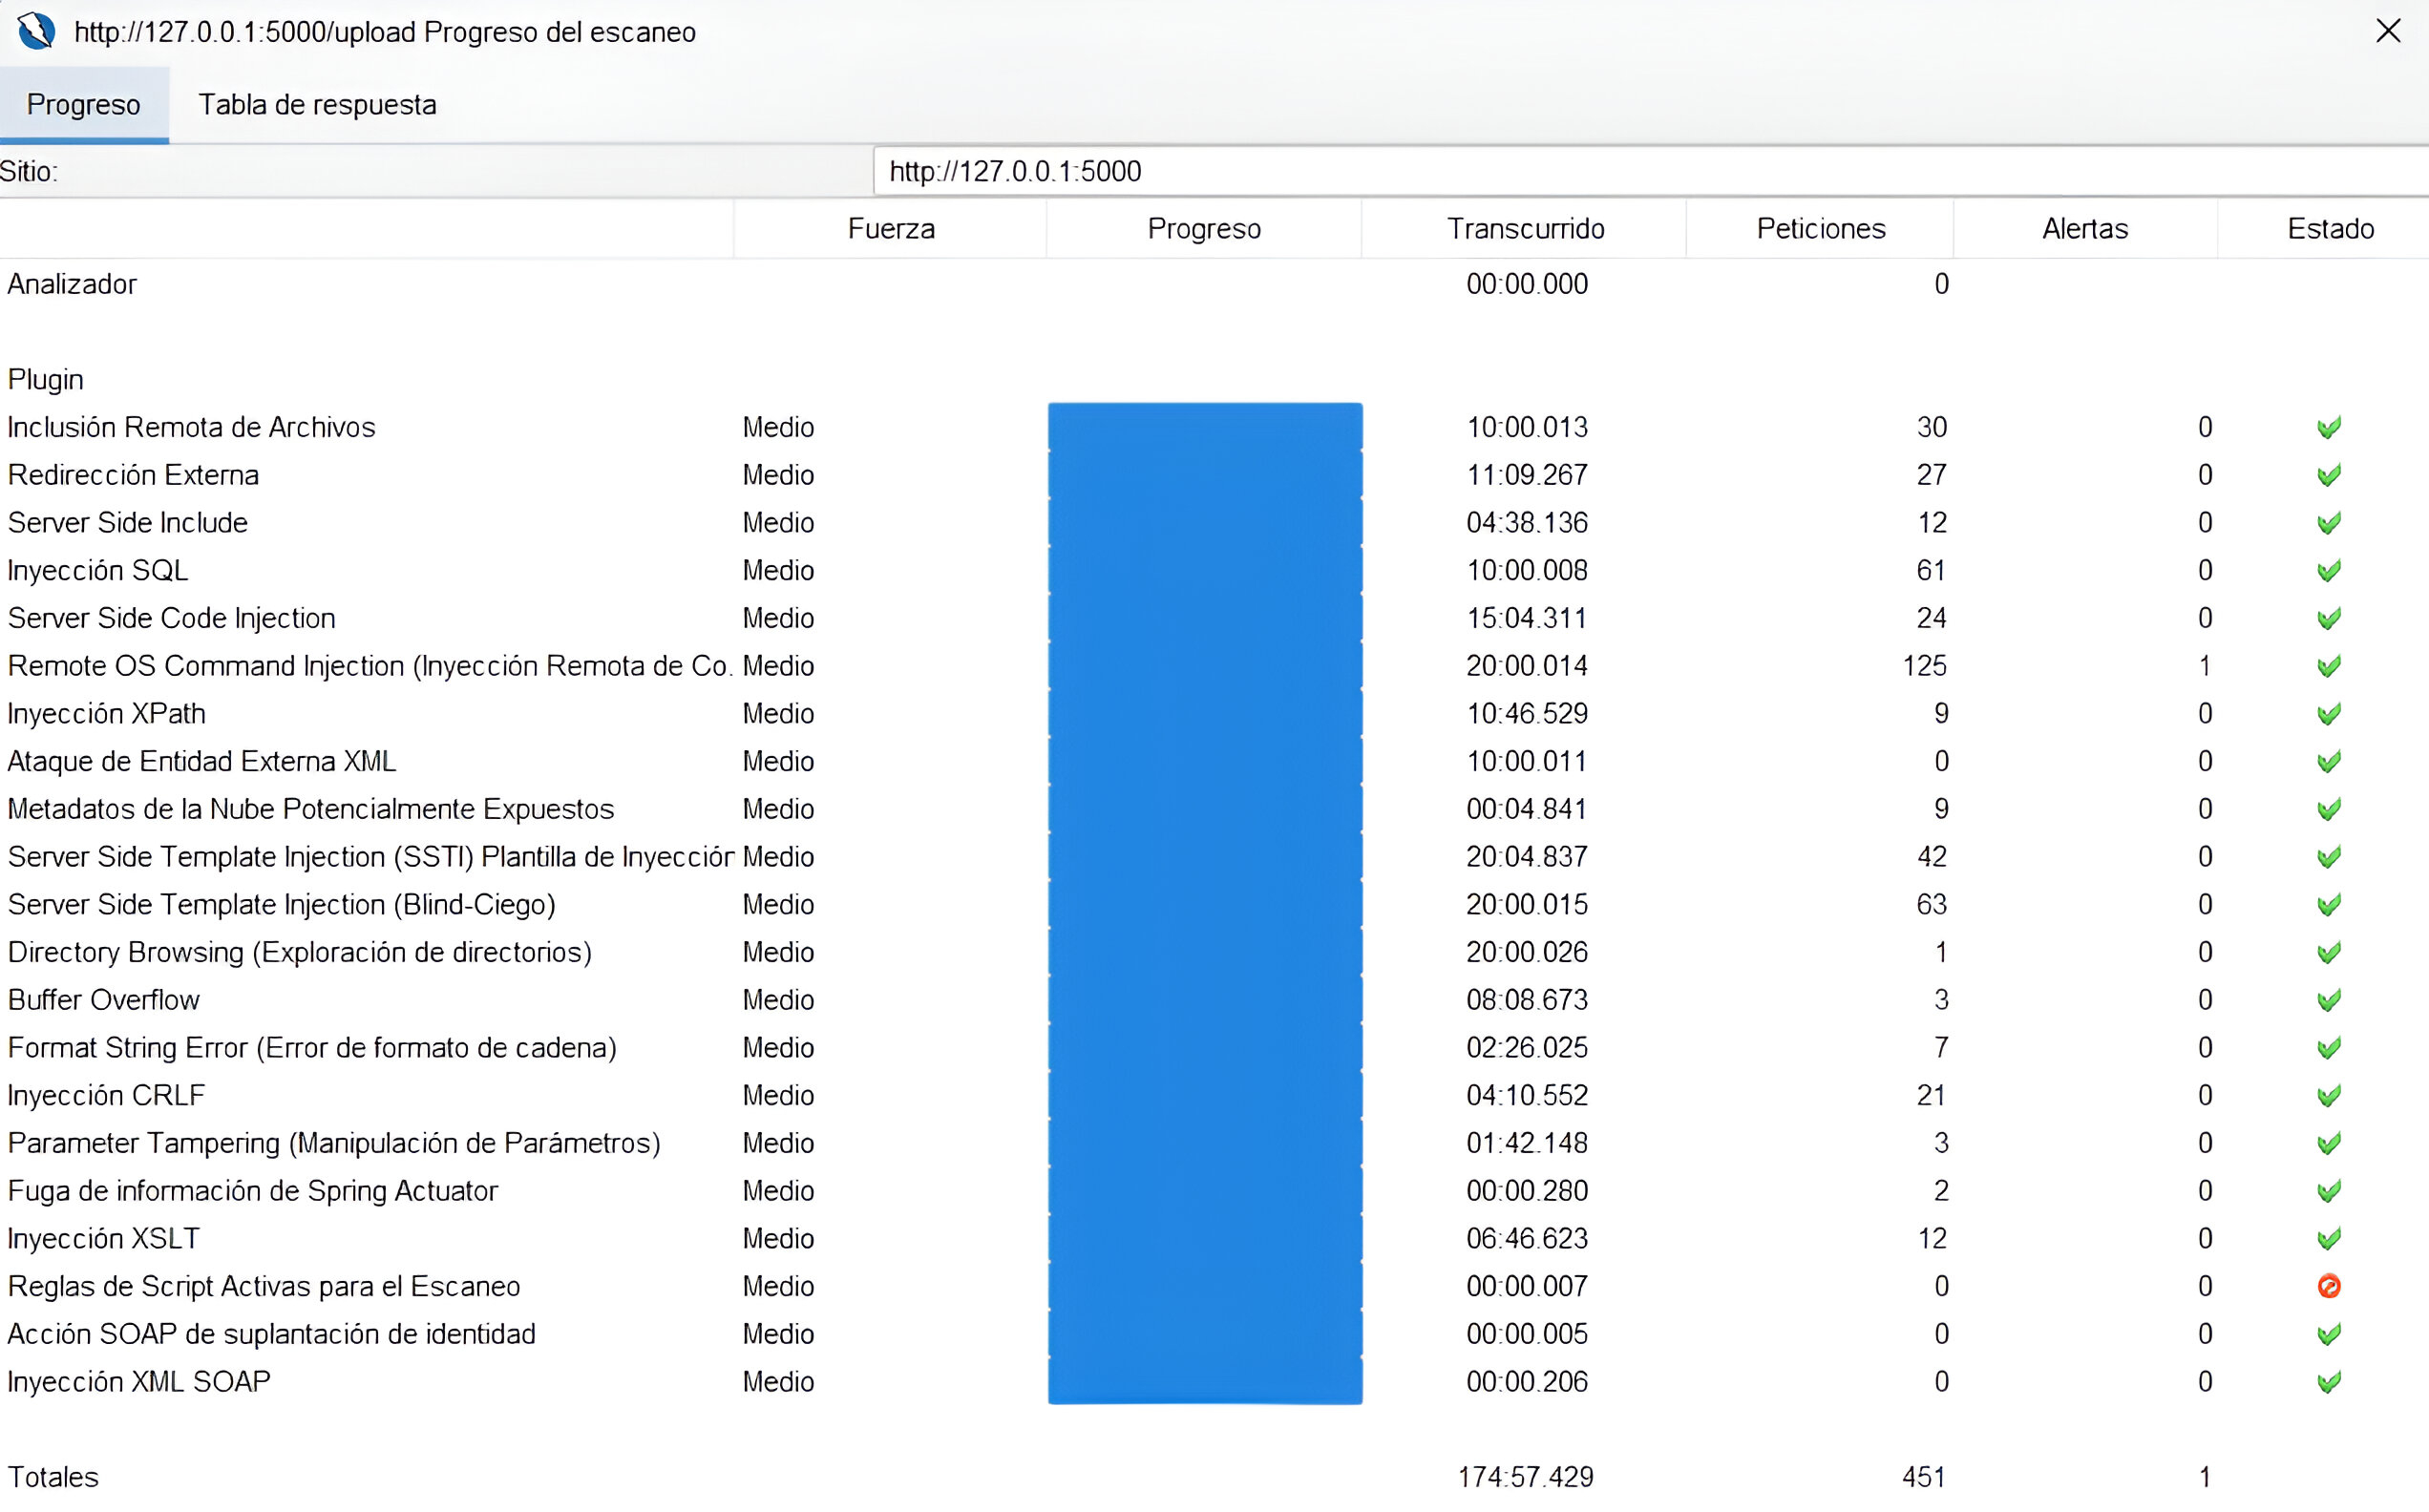
\includegraphics[width=1.0\textwidth]{figs/sec3D.jpg}
  \caption{Resultado de la prueba de seguridad sobre el endpoint del modelo generativo 3D del servidor}
  \label{fig:sec3D}
\end{figure}
En este caso, ZAP ejecutó un ataque utilizando el payload \verb|captured.jpeg';sleep 15;'|, cuya finalidad es introducir un retraso deliberado en el sistema. La herramienta interpretó la latencia observada en la respuesta como una confirmación de éxito del ataque, sin embargo, al revisar detalladamente los resultados, se observó que el servidor devolvió correctamente el modelo 3D en formato \verb|.glb|, sin ninguna anomalía funcional o sintáctica como ilustra la Figura \ref{fig:secVuln4} en la que se puede observar el cuerpo de la respuesta HTTP con los datos binarios del archivo \verb|.glb|.

% Imagen S5
\begin{figure}[h!tb]
  \centering
  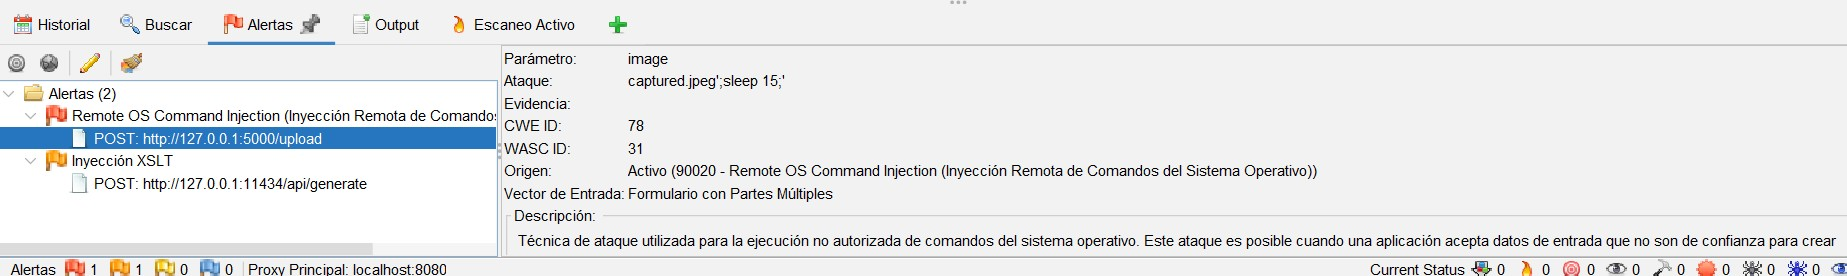
\includegraphics[width=1.0\textwidth]{figs/secVuln3.jpg}
  \caption{Vulnerabilidades obtenidas en el modelo generativo 3D}
  \label{fig:secVuln3}
\end{figure}

% Imagen S6
\begin{figure}[h!tb]
  \centering
  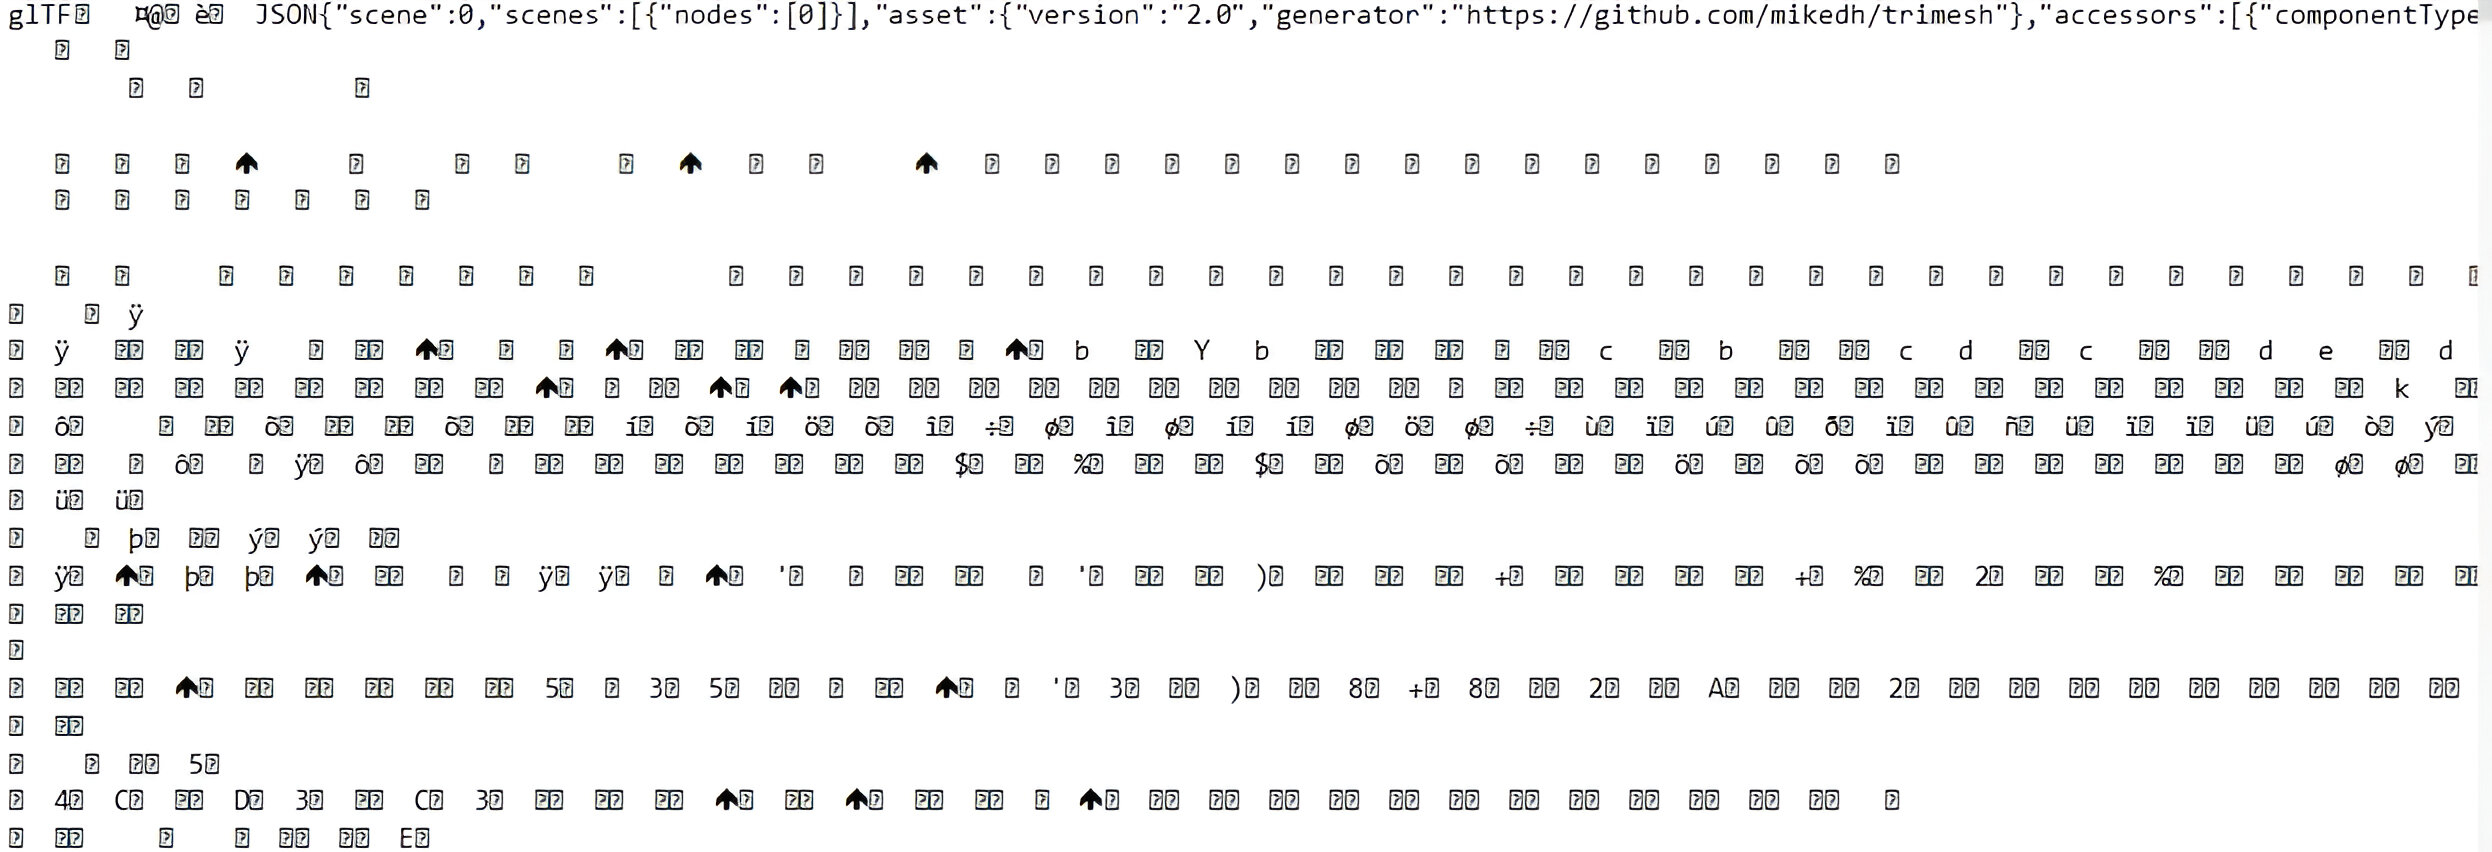
\includegraphics[width=1.0\textwidth]{figs/secVuln4.jpg}
  \caption{Detalles de la vulnerabilidad encontrada en el cuerpo de la respuesta HTTP del modelo generativo 3D}
  \label{fig:secVuln4}
\end{figure}

Adicionalmente, se intentó replicar manualmente el ataque utilizando comandos explícitos como \verb|pwd|, sin obtener ningún efecto observable, lo que sugiere que la advertencia reportada por ZAP se debe a una falsa correlación entre el tiempo de respuesta y la ejecución del comando \verb|sleep|. Dado que las pruebas de rendimiento han demostrado que el modelo generativo 3D requiere un mínimo de 40 segundos por inferencia en el mejor de los casos al estar ejecutándose en un hardware limitado, el retardo detectado por ZAP excede el umbral de los 15 segundos definidos en el payload, produciendo un falso positivo en la interpretación del test de inyección.






\chapter{Conclusiones}
% % Contenidos del capítulo.
% Las secciones presentadas son orientativas y no representan
% necesariamente la organización que debe tener este capítulo.

Este capítulo se estructura en tres apartados fundamentales. En primer lugar, se presenta un análisis comparativo entre la planificación inicial y los resultados obtenidos, tanto en términos de costes temporales como económicos, evaluando las posibles desviaciones respecto a las estimaciones realizadas durante la fase de planificación del proyecto. En segundo lugar, se lleva a cabo una evaluación y reflexión crítica sobre los resultados alcanzados tras la finalización del \gls{tfg}. Finalmente, se exponen una serie de líneas de mejora y elementos no abordados en el presente desarrollo, los cuales podrían ser considerados en futuros trabajos.

\section{Revisión de costes}

Al culminar un proyecto, es imprescindible reevaluar los costes reales que se han incurrido. Estos costes se clasifican en costes temporales y costes correspondientes al personal y recursos. En lo que respecta a los costes temporales, este \gls{tfg} tenía previsto un tiempo de desarrollo de entre 292 y 322 horas, incluyendo un 10\% adicional para imprevistos, y finalmente se completó en 294 horas. Esto es equivalente a 24 semanas y media o 5 meses y medio, comenzando el trabajo en enero y concluyéndolo a mediados de junio del año 2025. La estimación original consideraba una serie de riesgos y medidas para absorber posibles retrasos, y dado que el autor ya tenía el proyecto bastante adelantado antes de adoptarlo como \gls{tfg}, el tiempo de desarrollo final estuvo casi conforme a la predicción inicial.

Entre los riesgos identificados, uno era la posible falta de integración entre el complemento de Blender, el proxy y la API desarrollada con Flask. Sin embargo, esta integración se completó dentro del tiempo previsto y se solucionaron todos los problemas de comunicación. Otro posible riesgo involucraba dificultades en la configuración de Docker y Docker Compose al momento de desplegar el clúster. Afortunadamente, la validación y depuración del despliegue se efectuaron suavemente ajustando los archivos de configuración dentro del plazo estimado. Además, existía el riesgo de fallos en la conversión de imágenes a modelos 3D. Para abordar esto, se hicieron ajustes en los hiperparámetros del modelo generativo TripoSR, como "Foreground Ratio", lo que resultó en modelos más nítidos sin excesivo ruido, respetando el tiempo asignado. Un riesgo más era el bajo rendimiento del modelo \gls{llm} utilizado. A pesar de partir de un modelo \gls{llm} destilado que ya ofrecía un buen rendimiento, se buscaron mejoras adicionales optimizando los parámetros de la imagen de Docker. Esto fue necesario ya que tener múltiples contenedores de modelos de \gls{ia} ejecutándose en paralelo con Docker Compose presentaba desafíos para mantener la estabilidad del rendimiento en el mismo equipo. Por último, entre los riesgos identificados durante el desarrollo del proyecto, destacan principalmente, la curva de aprendizaje asociada al uso de tecnologías y herramientas inicialmente desconocidas y por otro, la limitación de tiempo disponible debido a compromisos personales y académicos, como las prácticas profesionales, la carga lectiva del curso y las responsabilidades asumidas como delegado de 4.º del \gls{gim}. Estos factores finalmente no incrementaron en gran medida la finalización del \gls{tfg} respecto a la planificación inicial. En particular, la necesidad de adquirir conocimientos sobre la mayoría de las tecnologías utilizadas y en conjunto con la gestión simultánea de múltiples tareas ajenas al \gls{tfg}, representaron los riesgos más complejos de controlar, no obstante, se logró mantener estos factores bajo control, permitiendo que la duración del proyecto se mantuviera dentro del marco temporal previsto.

En otro contexto, se encuentran los costes de personal. En esta área, se calculó un gasto de 4.711\texteuro\ para las 322 horas de trabajo previstas con un margen de error del 10\%, considerando un salario de 11\texteuro\ por hora. Dado que el proyecto en realidad se extendió más allá del mínimo estimado de 292 horas pero no superó el máximo pronosticado de 322 horas, podemos afirmar que se completó en el tiempo previsto, alcanzando finalmente las 294 horas. Por lo tanto, es necesario recalcular los costes de personal basados en estas 294 horas, manteniendo la jornada laboral semanal original de 12 horas, resultando en un costo real de personal de 4.302\texteuro para el proyecto.

El segundo gasto a considerar es el referente a los materiales. Es necesario recalcular la amortización de cada material cuando se reduce el tiempo de utilización en el proyecto empleando otra vez la Fórmula \ref{eq:costematerial}. La Tabla~\ref{tab:coste_amortizacion_real} muestra el costo actualizado de amortización y el costo total de materiales para el proyecto.
% Tabla datos de costos y amortización de dispositivos
\begin{table}[H]
   \centering
   \begin{tabular}{|>{\centering\arraybackslash}p{4cm}|c|c|c|}
      \hline
      \textbf{Elemento}                             & \textbf{Coste}     & \textbf{Meses de utilización} & \textbf{Coste de Amortización} \\ \hline
      Ordenador portátil MSI Pulse GL66 12UEK-085ES & 1.340,00 \texteuro & 5,64                          & 157,45 \texteuro               \\ \hline
   \end{tabular}
   \caption{Datos de costes y amortización de dispositivos al finalizar el proyecto}
   \label{tab:coste_amortizacion_real}
\end{table}


En conclusión, la Tabla~\ref{tab:costos_reales} presenta el costo total de cada activo empleado en el proyecto, abarcando materiales, equipos de desarrollo y personal. Al final, se logró una reducción en los costes de 510,90\texteuro\ en comparación con lo previsto, esto se debe a que los costes estimados estaban calculados incluyendo un 10\% adicional de tiempo para imprevistos y finalmente se acabó empleando menos de ese tiempo adicional.
% Tabla desglose de costos
\begin{table}[H]
   \centering
   \begin{tabular}{|>{\centering\arraybackslash}p{8cm}|>{\centering\arraybackslash}p{3cm}|}
      \hline
      \textbf{Elemento}                                & \textbf{Coste (\texteuro)}  \\
      \hline
      Amortización portátil MSI Pulse GL66 12UEK-085ES & 157,45 \texteuro            \\
      \hline
      Recursos humanos                                 & 4.302,00 \texteuro          \\
      \hline
      \textbf{Total costes directos}                   & 4.459,45 \texteuro          \\
      \hline
      \textbf{OverHead costes indirectos (20\%)}       & 891,89 \texteuro            \\
      \hline
      \textbf{Total}                                   & \textbf{5.351,34 \texteuro} \\
      \hline
   \end{tabular}
   \caption{Desglose de costes al finalizar el proyecto}
   \label{tab:costos_reales}
\end{table}

\section{Conclusiones}

El presente \gls{tfg} ha tenido como objetivo el diseño e implementación de un complemento funcional para Blender, construido sobre una arquitectura de microservicios y desplegado mediante Docker Compose. La solución desarrollada integra tanto un modelo \gls{llm} utilizando Ollama, como un servicio personalizado de generación 3D a partir de imágenes, ambos accesibles a través de un proxy y de una API implementada con Flask.

Durante la fase inicial, se realizó un análisis comparativo entre distintas tecnologías de virtualización con contenedores (Docker, Docker Compose) y frameworks de microservicios, concluyendo con la adopción de Flask por su ligereza y facilidad de integración. Esta elección permitió garantizar tanto la portabilidad de la solución como el aislamiento de sus dependencias.

El proceso de implementación integró de forma efectiva competencias adquiridas en diversas asignaturas del grado. Los conocimientos de Bases de Datos y Sistemas de Información resultaron esenciales para la gestión de los metadatos de configuración, mientras que los contenidos abordados en Programación Hipermedia facilitaron la automatización de scripts de despliegue. Por su parte, las asignaturas de Redes Multimedia y Fundamentos de Redes de Computadores proporcionaron la base teórica y práctica para el diseño de la red interna utilizada en el entorno de Docker. El desarrollo del cliente API en Python fue posible gracias a la formación en Programación, y el diseño funcional del add-on se apoyó en los principios adquiridos en la asignatura de Animación.

La fase de análisis se apoyó en técnicas propias de la Ingeniería del Software, mediante las cuales se definieron los casos de uso y se elaboraron los diagramas de secuencia y clases, los cuales sirvieron como base para el diseño detallado de los componentes, interfaces y arquitectura de despliegue. La planificación temporal y presupuestaria fue respaldada por el uso de diagramas de Gantt y técnicas de gestión de proyectos adquiridas en la propia asignatura de Gestión de Proyectos del grado.

En cuanto a la validación del sistema, se aplicó una estrategia de pruebas estructurada que incluyó tanto pruebas unitarias (en forma de caja blanca) como pruebas de integración y funcionales (caja negra), verificando así el cumplimiento de los requisitos establecidos.

Finalmente, la fase de implementación no solo permitió consolidar conocimientos previos, sino que también facilitó la adquisición de nuevas competencias en tecnologías como Flask, Docker, Docker Compose y en orquestación de servicios de \gls{ia}. Los resultados obtenidos confirman que el add-on desarrollado constituye una herramienta útil para optimizar los flujos de trabajo en Blender, especialmente en tareas que involucran automatización y generación asistida por IA.

\section{Trabajo futuro}

A lo largo del desarrollo de este \gls{tfg}, han emergido varias líneas de mejora e investigación que, aunque no se abordan dentro del alcance de los objetivos actuales, son propuestas valiosas para futuras ampliaciones del complemento de Blender. A continuación, se detallan estas ideas que podrían emprenderse en proyectos futuros, utilizando la plataforma ya establecida:

\begin{itemize}
   \item \textbf{Despliegue de un clúster para servicios IA}

         Plantear el uso de orquestadores como Kubernetes para escalar dinámicamente las réplicas de los servicios \gls{llm} y 3D, distribuyendo la carga entre múltiples nodos y mejorando la tolerancia a fallos.
   \item \textbf{Integración con repositorios de prompts}

         Diseñar una base de datos colaborativa o un sistema de versionado (por ejemplo Git) para almacenar, compartir y valorar prompts de generación de código y de modelos 3D, facilitando su reutilización y mejora continua.
   \item \textbf{Optimización automática de prompts}

         Investigar algoritmos de refuerzo o aprendizaje supervisado que ajusten de forma iterativa los parámetros de entrada (prompts, hiperparámetros del modelo) para maximizar la calidad del código generado y la fidelidad geométrica del modelo 3D.
   \item \textbf{Vista previa en tiempo real}

         Desarrollar un mecanismo de streaming de resultados parciales desde los microservicios a Blender, permitiendo al usuario visualizar avances en la generación de la malla 3D mientras el proceso aún está en ejecución.
   \item \textbf{Soporte de múltiples back-ends de IA}

         Ampliar la arquitectura para incorporar otros proveedores \gls{llm} (locales o en la nube) y distintos motores de generación 3D.
   \item \textbf{Página Web propia del Add-on}

         Desarrollar un sitio web donde se detalle el funcionamiento e instalación del complemento y se ofrezca acceso para probar los modelos de \gls{ia} directamente en el mismo sitio web.
   \item \textbf{Dashboard de métricas y monitorización}

         Crear un panel web que recoja estadísticas de uso (tiempos de respuesta, aciertos del modelo, fallos), monitorice el estado de los contenedores y alerte ante cuellos de botella o errores en los servicios.
   \item \textbf{Pruebas de usabilidad con usuarios finales}

         Realizar estudios formales de ergonomía y experiencia de usuario para evaluar la facilidad de uso del add-on, identificar puntos de mejora en la interfaz y validar la adopción en flujos de trabajo profesionales.
   \item \textbf{Extensión a otros formatos de exportación}

         Incorporar la función de exportar modelos 3D no solo en formato .glb, sino también en otros formatos adicionales.
\end{itemize}



\printbibliography[heading=bibnumbered, title={Bibliografía \label{chap:bibliography}}]


\pagestyle{appendix}

\appendix

\chapter{Glosarios}
%\addcontentsline{toc}{chapter}{Acrónimos}
%\printnoidxglossary[type=\acronymtype, title=Acrónimos y abreviaciones, toctitle=Acrónimos y abreviaciones]
\printnoidxglossary[type=\acronymtype, title=Acrónimos y abreviaciones]

%\section{Términos}

\printnoidxglossary[type=main,title=Términos]
%\addcontentsline{toc}{chapter}{Glosario}
%\printnoidxglossary[type=main,title=Términos, toctitle=Términos]

% \chapter{Ficheros del Add-on}
\section{Código Python principal del Add-on}
\label{sec:puntoA1}

\captionsetup{type=listing}
\captionof{listing}{Código python (init.py) principal del panel del add-on.}
\label{lst:panelAddon1}
\begin{minted}[breaklines, fontsize=\small, linenos]{python}
    bl_info = {
        "name": "Chatbot + Generative 3D Assistant",
        "description": "Integra un LLM (streaming/ multihilo) con un Generador 3D en Blender",
        "author": "Víctor Sanz García",
        "version": (0, 7),
        "blender": (3, 6, 0),
        "category": "3D View",
    }
    
    import bpy
    import os
    import threading
    import queue
    import tempfile
    import shutil
    import requests
    import re
    
    from bpy.props import StringProperty
    
    # ----------------------------------------------------------------
    # 1) CÓDIGO DE LLM (streaming + multihilo), FILTRADO DE BARRAS DE CÓDIGO
    # ----------------------------------------------------------------
    
    q = queue.Queue()
    
    # Indicador global para saber si estamos dentro de un bloque de código
    in_code_block = False
    code_python = ""  # Acumula todo el markdown recibido
    code_blocks = []   # Acumula bloques de código extraídos
    
    if __name__ == "blender_GPT":
        from . import streamchatbot
    else:
        import streamchatbot
        from importlib import reload
        reload(streamchatbot)
    
    def extraer_codigo_python():
        """Extrae bloques de código Python del markdown acumulado"""
        global code_python, code_blocks
        
        # Usa el mismo patrón pero con flags para multilínea
        patron = re.compile(r'```[Pp]ython\s*(.*?)```', re.DOTALL)
        bloques = patron.findall(code_python)
        
        # Filtra solo nuevos bloques que no hayamos procesado
        nuevos_bloques = [b.strip() for b in bloques if b.strip() not in code_blocks]
        
        # Actualiza la lista de bloques conocidos
        code_blocks.extend(nuevos_bloques)
        
        return "\n\n".join(nuevos_bloques)
    
    def write_chat(chunk):
        """
        - Toma el fragmento 'chunk' (en Markdown).
        - Filtra para extraer solo las líneas que estén dentro de bloques
          de código (``` ... ```), ignorando todo lo demás.
        - Escribe esas líneas en un Text Editor "ChatBot_Output" y las concatena
          también en scene.response.
        """
        global in_code_block, code_python
    
        text_name = "ChatBot_Output"
    
        # 1) Crear u obtener el Text datablock
        if text_name not in bpy.data.texts:
            text = bpy.data.texts.new(text_name)
            if not bpy.app.background:
                # Abrir el Text Editor
                bpy.ops.screen.userpref_show('INVOKE_DEFAULT')
                for win in bpy.context.window_manager.windows:
                    if win.screen:
                        for area in win.screen.areas:
                            if area.type == 'PREFERENCES':
                                area.ui_type = 'TEXT_EDITOR'
                                area.spaces.active.text = text
        else:
            text = bpy.data.texts[text_name]
    
        # 2) Acumular chunk y extraer código
        global code_python
        code_python += chunk
        
        # Extraer nuevos bloques de código
        nuevo_codigo = extraer_codigo_python()
        
        # 3) Escribir solo si hay nuevo código
        if nuevo_codigo:
            text.write(nuevo_codigo)
            
            # Actualizar solo con el código nuevo
            try:
                scene = bpy.context.scene
                scene.response += nuevo_codigo
            except Exception:
                pass
    
        # 4) Forzar redraw del Text Editor
        for area in bpy.context.screen.areas:
            if area.type == 'TEXT_EDITOR' and area.spaces.active.text == text:
                area.tag_redraw()
    
    
    @bpy.app.handlers.persistent
    def process_queue():
        """
        Timer que se ejecuta cada 0.1 s para vaciar la cola 'q'.
        Cada chunk se manda a write_chat(chunk).
        """
        try:
            while not q.empty():
                chunk = q.get_nowait()
                write_chat(chunk)
        except queue.Empty:
            pass
    
        return 0.1  # Indicamos que queremos volver a ser llamado en 0.1s
    
    
    class ChatBotGenerateOperator(bpy.types.Operator):
        """
        Operador que se dispara al pulsar "Generar código".
        Lanza un hilo que corre create_chat_bot() (que streamea Markdown).
        write_chat() filtrará solo el código Python dentro de ```...```.
        """
        bl_idname = "chatbot.generate_code"
        bl_label = "Generar código"
        bl_description = "Envía el prompt al LLM en un hilo, con streaming"
    
    
        def invoke(self, context, event):
            global in_code_block, code_python, code_blocks
            
            scene = context.scene
            
            # 1) Limpiar respuesta previa y estado
            scene.response = ""
            code_python = ""  # Reiniciar acumulador
            code_blocks = []  # Reiniciar bloques conocidos
    
            # 1) Limpiar respuesta previa y estado de bloques de código
            text_name = "ChatBot_Output"
            if text_name in bpy.data.texts:
                bpy.data.texts.remove(bpy.data.texts[text_name])
            in_code_block = False
    
            # 2) Lanzar el hilo de streaming
            prompt = scene.prompt
            thread = threading.Thread(
                target=streamchatbot.create_chat_bot,
                args=(prompt, "", q)
            )
            thread.daemon = True
            thread.start()
    
            return {'FINISHED'}
    
    
    class ChatBotExecuteOperator(bpy.types.Operator):
        """
        Ejecuta en Blender el código Python que ya está filtrado en scene.response.
        """
        bl_idname = "chatbot.execute_code"
        bl_label = "Ejecutar código"
        bl_description = "Ejecuta en Blender el código generado por el LLM"
    
        def execute(self, context):
            scene = context.scene
            code = scene.response
    
            try:
                exec(code, {'bpy': bpy})
                self.report({'INFO'}, "Código ejecutado correctamente")
            except Exception as e:
                self.report({'ERROR'}, f"Error al ejecutar código: {str(e)}")
    
            return {'FINISHED'}
    
    
    # ----------------------------------------------------------------
    # 2) PROPIEDADES DE SCENE
    # ----------------------------------------------------------------
    
    def init_properties():
        # 2.1) PROPS PARA LLM
        bpy.types.Scene.prompt = StringProperty(
            name="Prompt LLM",
            description="¿Qué acción quieres hacer en Blender?",
            default=""
        )
        bpy.types.Scene.response = StringProperty(
            name="Respuesta LLM",
            description="Aquí aparecerá únicamente el código Python que llegue por streaming",
            default="",
        )
    
        # 2.2) PROPS PARA AGENTE 3D
        bpy.types.Scene.gc_image_path = StringProperty(
            name="Ruta de Imagen",
            description="Ruta de la imagen para generar el modelo 3D",
            default="",
            subtype='FILE_PATH'
        )
        bpy.types.Scene.gc_image_name = StringProperty(
            name="Nombre de Imagen",
            description="Nombre del datablock de la imagen cargada (para preview)",
            default="",
        )
        bpy.types.Scene.gc_model_path = StringProperty(
            name="Ruta de Modelo 3D",
            description="Ruta del archivo 3D generado (.glb)",
            default="",
            subtype='FILE_PATH'
        )
        bpy.types.Scene.gc_status = StringProperty(
            name="Estado Generación",
            description="Estado del proceso de generación 3D",
            default=""
        )
    
    
    def clear_properties():
        # 2.1) LIMPIAR PROPS LLM
        if hasattr(bpy.types.Scene, "prompt"):
            delattr(bpy.types.Scene, "prompt")
        if hasattr(bpy.types.Scene, "response"):
            delattr(bpy.types.Scene, "response")
    
        # 2.2) LIMPIAR PROPS AGENTE 3D
        if hasattr(bpy.types.Scene, "gc_image_path"):
            delattr(bpy.types.Scene, "gc_image_path")
        if hasattr(bpy.types.Scene, "gc_image_name"):
            delattr(bpy.types.Scene, "gc_image_name")
        if hasattr(bpy.types.Scene, "gc_model_path"):
            delattr(bpy.types.Scene, "gc_model_path")
        if hasattr(bpy.types.Scene, "gc_status"):
            delattr(bpy.types.Scene, "gc_status")
    
    
    # ----------------------------------------------------------------
    # 3) OPERADORES DEL AGENTE 3D
    # ----------------------------------------------------------------
    
    class GC_OT_CargarImagen(bpy.types.Operator):
        bl_idname = "gc.cargar_imagen"
        bl_label = "Cargar imagen"
        bl_description = "Selecciona una imagen para generar el modelo 3D"
        filepath: StringProperty(subtype="FILE_PATH")
    
        def execute(self, context):
            scene = context.scene
            path = self.filepath
    
            if os.path.isfile(path):
                try:
                    img = bpy.data.images.load(path)
                    scene.gc_image_path = path
                    scene.gc_image_name = img.name
                    self.report({'INFO'}, "Imagen cargada correctamente")
                except Exception as e:
                    self.report({'ERROR'}, f"Error al cargar imagen: {str(e)}")
            else:
                self.report({'ERROR'}, "La ruta no es válida")
    
            return {'FINISHED'}
    
        def invoke(self, context, event):
            context.window_manager.fileselect_add(self)
            return {'RUNNING_MODAL'}
    
    
    class GC_OT_GenerarModelo3D(bpy.types.Operator):
        bl_idname = "gc.generar_modelo_3d"
        bl_label = "Generar modelo 3D"
        bl_description = "Envía la imagen al servicio 3D y obtiene un archivo GLB de forma no bloqueante"
    
        def invoke(self, context, event):
            scene = context.scene
            image_path = scene.gc_image_path
    
            if not os.path.isfile(image_path):
                self.report({'ERROR'}, "Primero debes cargar una imagen")
                return {'CANCELLED'}
    
            # Limpiar modelo previo
            scene.gc_model_path = ""
    
            # Lanzar hilo para petición HTTP
            thread = threading.Thread(
                target=self.threaded_request_glb,
                args=(image_path,)
            )
            thread.daemon = True
            thread.start()
    
            self.report({'INFO'}, "Petición enviada al servicio 3D (en background)")
            return {'FINISHED'}
    
        def threaded_request_glb(self, image_path):
            try:
                url = "http://127.0.0.1:5000/upload"
                files = {'image': open(image_path, 'rb')}
                response = requests.post(url, files=files, timeout=900)
                response.raise_for_status()
    
                temp_dir = tempfile.gettempdir()
                filename = os.path.join(temp_dir, "gc_model.glb")
                with open(filename, 'wb') as f:
                    f.write(response.content)
    
                # Actualizar en el hilo principal usando propiedades
                def update_success():
                    scene = bpy.context.scene
                    scene.gc_model_path = filename
                    scene.gc_status = f"Modelo 3D generado: {os.path.basename(filename)}"
                    return None
                    
                bpy.app.timers.register(update_success)
    
            except Exception as e:
                # Manejar errores usando propiedades
                def update_error():
                    scene = bpy.context.scene
                    scene.gc_status = f"Error: {str(e)}"
                    return None
                    
                bpy.app.timers.register(update_error)
    
    
    class GC_OT_CargarModelo(bpy.types.Operator):
        bl_idname = "gc.cargar_modelo"
        bl_label = "Cargar modelo"
        bl_description = "Importa el modelo 3D (.glb) generado en la escena"
    
        def execute(self, context):
            scene = context.scene
            model_path = scene.gc_model_path
    
            if not os.path.isfile(model_path):
                self.report({'ERROR'}, "No hay un modelo 3D generado aún")
                return {'CANCELLED'}
    
            try:
                bpy.ops.import_scene.gltf(filepath=model_path)
                self.report({'INFO'}, "Modelo 3D (.glb) importado en la escena")
            except Exception as e:
                self.report({'ERROR'}, f"Error al importar modelo: {str(e)}")
    
            return {'FINISHED'}
    
    
    class GC_OT_DescargarModelo(bpy.types.Operator):
        bl_idname = "gc.descargar_modelo"
        bl_label = "Descargar modelo"
        bl_description = "Guarda una copia del modelo 3D en la ubicación que elijas"
        filepath: StringProperty(subtype="FILE_PATH")
    
        def execute(self, context):
            scene = context.scene
            src = scene.gc_model_path
            dest = self.filepath
    
            if not os.path.isfile(src):
                self.report({'ERROR'}, "No hay un modelo 3D para descargar")
                return {'CANCELLED'}
    
            try:
                shutil.copy(src, dest)
                self.report({'INFO'}, f"Modelo guardado en: {dest}")
            except Exception as e:
                self.report({'ERROR'}, f"Error al guardar modelo: {str(e)}")
    
            return {'FINISHED'}
    
        def invoke(self, context, event):
            if not os.path.isfile(context.scene.gc_model_path):
                self.report({'ERROR'}, "No hay un modelo 3D para descargar")
                return {'CANCELLED'}
            context.window_manager.fileselect_add(self)
            return {'RUNNING_MODAL'}
    
    
    # ----------------------------------------------------------------
    # 4) PANEL PRINCIPAL: AGENTE LLM + AGENTE 3D
    # ----------------------------------------------------------------
    
    class ChatBotPanel(bpy.types.Panel):
        bl_label = "GenerativeCHAT"
        bl_idname = "CHATBOT_PT_panel"
        bl_space_type = 'VIEW_3D'
        bl_region_type = 'UI'
        bl_category = "GenerativeCHAT"
    
        def draw(self, context):
            layout = self.layout
            scene = context.scene
    
            # ==== AGENTE LLM ====
            box_llm = layout.box()
            box_llm.label(text="AGENTE LLM", icon='NODE')
    
            # Input de prompt + botón "Generar código"
            row = box_llm.row(align=True)
            row.prop(scene, "prompt", text="")
            row.operator("chatbot.generate_code", text="Generar código", icon='FILE_SCRIPT')
    
            box_llm.separator()
    
            # Área multiline con la respuesta (solo código Python)
            box_llm.prop(scene, "response", text="")
    
            # Botón "Ejecutar código"
            box_llm.operator("chatbot.execute_code", text="Ejecutar código", icon='PLAY')
    
            # ==== AGENTE 3D ====
            box_3d = layout.box()
            box_3d.label(text="AGENTE 3D", icon='MESH_CUBE')
    
            if scene.gc_status:
                box_3d.label(text=scene.gc_status, icon='INFO')
    
            row3 = box_3d.row()
    
            col_a = row3.column()
            if scene.gc_image_name != "":
                img = bpy.data.images.get(scene.gc_image_name)
                if img:
                    col_a.template_preview(img, show_buttons=False)
            col_a.operator("gc.cargar_imagen", text="Cargar imagen", icon='IMAGE_DATA')
    
            col_b = row3.column()
            col_b.operator("gc.generar_modelo_3d", text="Generar modelo 3D", icon='MOD_REMESH')
    
            if scene.gc_model_path != "":
                box_3d.separator()
                box_3d.label(text=f"Modelo 3D: {os.path.basename(scene.gc_model_path)}", icon='OBJECT_DATA')
                row4 = box_3d.row(align=True)
                row4.operator("gc.cargar_modelo", text="Cargar modelo", icon='IMPORT')
                row4.operator("gc.descargar_modelo", text="Descargar modelo", icon='EXPORT')
    
    
    # ----------------------------------------------------------------
    # 5) REGISTRO / DESREGISTRO
    # ----------------------------------------------------------------
    
    classes = (
        ChatBotGenerateOperator,
        ChatBotExecuteOperator,
        ChatBotPanel,
        GC_OT_CargarImagen,
        GC_OT_GenerarModelo3D,
        GC_OT_CargarModelo,
        GC_OT_DescargarModelo,
    )
    
    def register():
        for cls in classes:
            bpy.utils.register_class(cls)
        init_properties()
    
        # Registro del temporizador para procesar la cola de streaming
        bpy.app.timers.register(process_queue)
    
    
    def unregister():
        # Desregistrar temporizador
        try:
            bpy.app.timers.unregister(process_queue)
        except Exception:
            pass
    
        for cls in reversed(classes):
            bpy.utils.unregister_class(cls)
        clear_properties()
    
    
    if __name__ == "__main__":
        register()
\end{minted}


 
\captionsetup{type=listing}
\captionof{listing}{Código python (streamchatbot.py) generador del stream del chatbot.}
\label{lst:streamBotAddon}
\begin{minted}[breaklines, fontsize=\small, linenos]{python}
    import requests
    import json
    
    def is_json(myjson):
        try:
            json_object = json.loads(myjson)
            return True
        except ValueError as e:
            return False
    
    def create_chat_bot(prompt, key, q): 
        for chunk in chatbot(prompt, key):
            if chunk:
                q.put(chunk)
    
    def chatbot(pmt, key):
        url = "http://127.0.0.1:11434/api/generate"
        
        data = {
            "model": "dolphin-mistral:7b-v2.6-dpo-laser-q4_0",
            "prompt": pmt,
            "stream": True
        }
    
        print("\nTú:", pmt, end="\n\n")
        print("Blender_GPT:", end=" ")
    
        try:
            response = requests.post(url, json=data, stream=True, timeout=900)
            response.raise_for_status()
            
            for line in response.iter_lines():
                if line:
                    try:
                        json_data = json.loads(line)
                        if 'response' in json_data:
                            yield json_data['response']
                    except json.JSONDecodeError:
                        continue
                        
        except Exception as e:
            yield f"\nError: {str(e)}"
\end{minted}



\section{Fichero de inicialización del modelo LLM}
\label{sec:puntoA2}
% Bash
 
\captionsetup{type=listing}
\captionof{listing}{Script Bash (entrypoint.sh) de descarga e inicialización de Ollama y del modelo LLM.}
\label{lst:scriptOllama}
\begin{minted}[breaklines, fontsize=\small, linenos]{bash}
    #!/bin/sh
    
    # Inicia el servidor Ollama en segundo plano
    /bin/ollama serve &
    
    # Espera 20 segundos para que el servidor se inicie
    sleep 20
    
    # Verificar si el modelo está presente
    MODEL_NAME="dolphin-mistral:7b-v2.6-dpo-laser-q4_0"
    if ! ollama list | grep -q "$MODEL_NAME"; then
        echo "Descargando el modelo..."
        
        # Crear un lock file para evitar descargas concurrentes
        LOCK_FILE="/root/.ollama/model_download.lock"
        if [ ! -f "$LOCK_FILE" ]; then
            touch "$LOCK_FILE"
            ollama pull $MODEL_NAME
            rm -f "$LOCK_FILE"
        else
            # Esperar a que otro contenedor complete la descarga
            while [ -f "$LOCK_FILE" ]; do
                echo "Esperando que otro contenedor termine la descarga..."
                sleep 10
            done
        fi
    fi
    
    # Mantener el contenedor en ejecución
    tail -f /dev/null
\end{minted}



\section{Fichero de dependencias del modelo TripoSR}
\label{sec:puntoA3}
  % Quitar cuando esté referenciado
% Imagen requeriments.txt
\captionsetup{type=listing}
\captionof{listing}{Archivo (requirements.txt) de dependencias del modelo 3D.}
\label{lst:dependencias3D}
\begin{minted}[breaklines, fontsize=\small, linenos]{text}
    flask
    flask-cors
    onnxruntime
    gunicorn
    omegaconf==2.3.0
    Pillow==10.1.0
    einops==0.7.0
    transformers==4.35.0
    trimesh==4.0.5
    rembg
    huggingface-hub
    imageio[ffmpeg]
\end{minted}



\section{Ficheros de la API del modelo TripoSR}
\label{sec:puntoA4}
% Código API modelo3d
 
\captionsetup{type=listing}
\captionof{listing}{Código python (app.py) de la API Flask del modelo 3D.}
\label{lst:appAPI3d}
\begin{minted}[breaklines, fontsize=\small, linenos]{python}
    from run import generate_geometry
    from flask import Flask, request, send_file
    from flask_cors import CORS
    import os
    import time
    
    app = Flask(__name__)
    CORS(app)
    
    def check_file_existence(directory, filename):
        """Function to check if a file exists in a directory."""
        return os.path.exists(os.path.join(directory, filename))
    
    @app.route('/upload', methods=['POST'])
    def upload_file():
        if 'image' in request.files:
            image = request.files['image']
            directory = 'output/0'
            filename_mesh = 'mesh.glb'
    
            # Lee los datos binarios de la imagen
            image_data = image.read()
            generate_geometry(image_data)  # Pasa los datos binarios
            
            return send_file(os.path.join(directory, filename_mesh), as_attachment=True, mimetype='model/gltf-binary')
        else:
            return 'No image provided', 400
    
    if __name__ == '__main__':
        app.run(host='0.0.0.0')
\end{minted}



\section{Fichero del modelo TripoSR}
\label{sec:puntoA5}
 
% Código modelo3d adaptado
\captionsetup{type=listing}
\captionof{listing}{Código python (run.py) que ejecuta el modelo 3D adaptado.}
\label{lst:runAPI3d}
\begin{minted}[breaklines, fontsize=\small, linenos]{python}
    import argparse
    import logging
    import os
    import time
    
    import numpy as np
    import rembg
    import torch
    from PIL import Image
    from io import BytesIO
    
    from tsr.system import TSR
    from tsr.utils import remove_background, resize_foreground, save_video
    
    def generate_geometry(image_web):
        class Timer:
            def __init__(self):
                self.items = {}
                self.time_scale = 1000.0  # ms
                self.time_unit = "ms"
    
            def start(self, name: str) -> None:
                if torch.cuda.is_available():
                    torch.cuda.synchronize()
                self.items[name] = time.time()
                logging.info(f"{name} ...")
    
            def end(self, name: str) -> float:
                if name not in self.items:
                    return
                if torch.cuda.is_available():
                    torch.cuda.synchronize()
                start_time = self.items.pop(name)
                delta = time.time() - start_time
                t = delta * self.time_scale
                logging.info(f"{name} finished in {t:.2f}{self.time_unit}.")
    
        timer = Timer()
    
        logging.basicConfig(
            format="%(asctime)s - %(levelname)s - %(message)s", level=logging.INFO
        )
    
        input_image = image_web      #"examples/chair.png"
        output_dir = "output/"
        device = "cuda:0"   #"cpu"
        pretrained = "stabilityai/TripoSR"
        chunksize = 8192
        noremove_bg = False
        foreground = 0.85
        resolution = 256
        model_format = "glb"    #"obj"
        render_store = False
    
        os.makedirs(output_dir, exist_ok=True)
    
        if not torch.cuda.is_available():
            device = "cpu"
    
        timer.start("Initializing model")
        model = TSR.from_pretrained(
            pretrained,
            config_name="config.yaml",
            weight_name="model.ckpt",
        )
        model.renderer.set_chunk_size(chunksize)
        model.to(device)
        timer.end("Initializing model")
    
        timer.start("Processing images")
        images = []
    
        if noremove_bg:
            rembg_session = None
        else:
            rembg_session = rembg.new_session()
    
        if noremove_bg:
            image = np.array(Image.open(BytesIO(input_image)).convert("RGB"))
        else:
            image = remove_background(Image.open(BytesIO(input_image)), rembg_session)
            image = resize_foreground(image, foreground)
            image = np.array(image).astype(np.float32) / 255.0
            image = image[:, :, :3] * image[:, :, 3:4] + (1 - image[:, :, 3:4]) * 0.5
            image = Image.fromarray((image * 255.0).astype(np.uint8))
            if not os.path.exists(os.path.join(output_dir, str(0))):
                os.makedirs(os.path.join(output_dir, str(0)))
            image.save(os.path.join(output_dir, str(0), f"input.png"))
        images.append(image)
        timer.end("Processing images")
    
        for i, image in enumerate(images):
            logging.info(f"Running image {i + 1}/{len(images)} ...")
    
            timer.start("Running model")
            with torch.no_grad():
                scene_codes = model([image], device=device)
            timer.end("Running model")
    
            if render_store:
                timer.start("Rendering")
                render_images = model.render(scene_codes, n_views=30, return_type="pil")
                for ri, render_image in enumerate(render_images[0]):
                    render_image.save(os.path.join(output_dir, str(i), f"render_{ri:03d}.png"))
                save_video(
                    render_images[0], os.path.join(output_dir, str(i), f"render.mp4"), fps=30
                )
                timer.end("Rendering")
    
            timer.start("Exporting mesh")
            meshes = model.extract_mesh(scene_codes, resolution=resolution)
            meshes[0].export(os.path.join(output_dir, str(i), f"mesh.{model_format}"))
            timer.end("Exporting mesh")
\end{minted}



\section{Dockerfile del modelo TripoSR}
\label{sec:puntoA6}
 
% Dockerfile modelo3d
\captionsetup{type=listing}
\captionof{listing}{Dockerfile de la imagen de Docker del servicio del modelo 3D.}
\label{lst:dockerfileM3D}
\begin{minted}[breaklines, fontsize=\small, linenos]{dockerfile}
    # Utiliza una imagen base de Python
    FROM python:3.8-slim
    
    # Establece el directorio de trabajo en el contenedor
    WORKDIR /app
    
    # Copia los archivos de la aplicación Flask al contenedor
    COPY . /app
    
    # Actualiza setuptools y luego instala las dependencias de Python
    RUN pip install --upgrade setuptools && pip install -r requirements.txt && pip install torch torchvision torchaudio -f https://download.pytorch.org/whl/torch_stable.html
    
    # Cambia al directorio del repositorio
    WORKDIR /app/torchmcubes
    
    RUN apt-get update && \
        apt-get install -y g++ ninja-build && \
        apt-get clean && \
        rm -rf /var/lib/apt/lists/*
    
    # Ejecuta el script de Python que genera la carpeta y el archivo .pyd
    RUN python setup.py build_ext -i
    
    # Mueve los archivos generados a la carpeta de librerías de Python
    RUN mv torchmcubes /usr/local/lib/python3.8/site-packages/torchmcubes && \
        mv build/lib.linux-x86_64-cpython-38/
        torchmcubes_module.cpython-38-x86_64-linux-gnu.so 
        /usr/local/lib/python3.8/site-packages/
    
    WORKDIR /app
    
    RUN rm -rf torchmcubes
    
    # Expone el puerto en el que se ejecutará la aplicación Flask
    EXPOSE 5000
    
    # Ejecuta la aplicación Flask con Gunicorn para producción
    CMD ["gunicorn", "-b", "0.0.0.0:5000", "--timeout", "1000", "app:app"]
\end{minted}



\chapter{Ficheros de despliegue local}
\section{Archivos de configuración}
\label{sec:puntoB1}
 
% docker-compose.yml
\captionsetup{type=listing}
\captionof{listing}{Archivo de configuración Docker-Compose del despliegue del servidor en local.}
\label{lst:composeServidor}
\begin{minted}[breaklines, fontsize=\small, linenos]{yaml}
    version: '3.8'
    
    services:
      ollama:
        image: ollama/ollama
        volumes:
          - ollama_data:/root/.ollama
          - ./ollama/entrypoint.sh:/entrypoint.sh
        entrypoint: /entrypoint.sh
        networks:
          - backend
        deploy:
          resources:
            limits:
              memory: 4G  # Más espacio para cargar modelos grandes
            reservations:
              memory: 1G
    
      modelo3d:
        build:
          context: ./modelo3d
        networks:
          - backend
        deploy:
          replicas: 2
          resources:
            limits:
              memory: 6G  # Más memoria para cada instancia
            reservations:
              memory: 3G
    
      nginx:
        image: nginx:alpine
        ports:
          - "11434:80"
          - "5000:5000"
        volumes:
          - ./nginx/nginx.conf:/etc/nginx/nginx.conf
        depends_on:
          - ollama
          - modelo3d
        networks:
          - backend
        environment:
          - NGINX_WORKER_PROCESSES=4
        deploy:
          resources:
            reservations:
              memory: 256M
    
    volumes:
      ollama_data:
    
    networks:
      backend:
        driver: bridge
\end{minted}

 
% nginx.conf
\captionsetup{type=listing}
\captionof{listing}{Archivo de configuración Nginx (nginx.conf) del proxy del servidor.}
\label{lst:nginxConfig}
\begin{minted}[breaklines, fontsize=\small, linenos]{nginx}
    events {
        worker_connections 1024;
    }
    
    http {
        # DNS de Docker para balanceo automático
        resolver 127.0.0.11 valid=10s;
    
        upstream ollama_servers {
            server ollama:11434;
        }
    
        upstream modelo3d_servers {
            server modelo3d:5000;
        }
    
        server {
            listen 80;
            
            location /api/generate {
                proxy_pass http://ollama_servers;
                proxy_http_version 1.1;
                proxy_set_header Host $host;
                proxy_set_header Connection '';
                
                # Timeouts extendidos
                proxy_connect_timeout       900;
                proxy_send_timeout          900;
                proxy_read_timeout          900;
                send_timeout                900;
            }
        }
    
        server {
            listen 5000;
            
            location /upload {
                proxy_pass http://modelo3d_servers;
                proxy_http_version 1.1;
                proxy_set_header Host $host;
                proxy_set_header Connection '';
                client_max_body_size        100M;
                
                # Timeouts extendidos para generación 3D
                proxy_connect_timeout       900;
                proxy_send_timeout          900;
                proxy_read_timeout          900;
                send_timeout                900;
            }
        }
    }
\end{minted}



\chapter{Resultados de pruebas}
\section{Resultados de las pruebas funcionales}
\label{sec:puntoC1}
% Imagen
  \begin{figure}[h!tb]
    \centering
    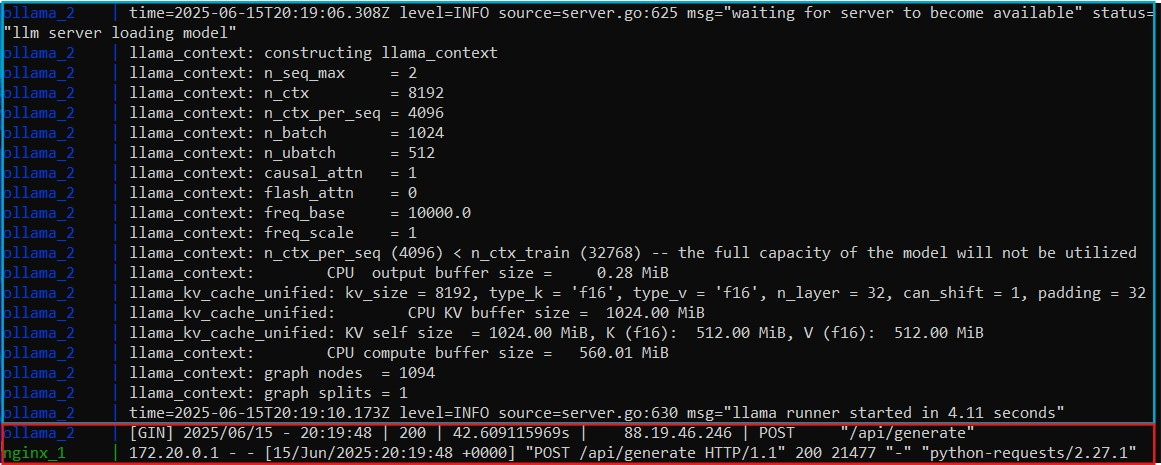
\includegraphics[width=0.8\textwidth]{figs/cu1cu8.jpg}
    \caption{Captura de pantalla del terminal de logs del servidor para el CU1 y CU8 en las pruebas funcionales}
    \label{fig:cu1cu8}
  \end{figure}

% Imagen
  \begin{figure}[h!tb]
    \centering
    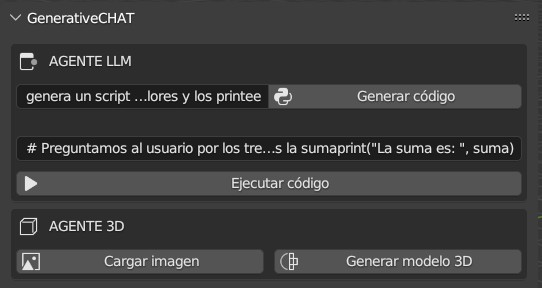
\includegraphics[width=0.8\textwidth]{figs/cu2_1.jpg}
    \caption{Captura de pantalla del campo de respuesta del modelo LLM en el add-on para el CU2 en las pruebas funcionales}
    \label{fig:cu2_1}
  \end{figure}

% Imagen
  \begin{figure}[h!tb]
    \centering
    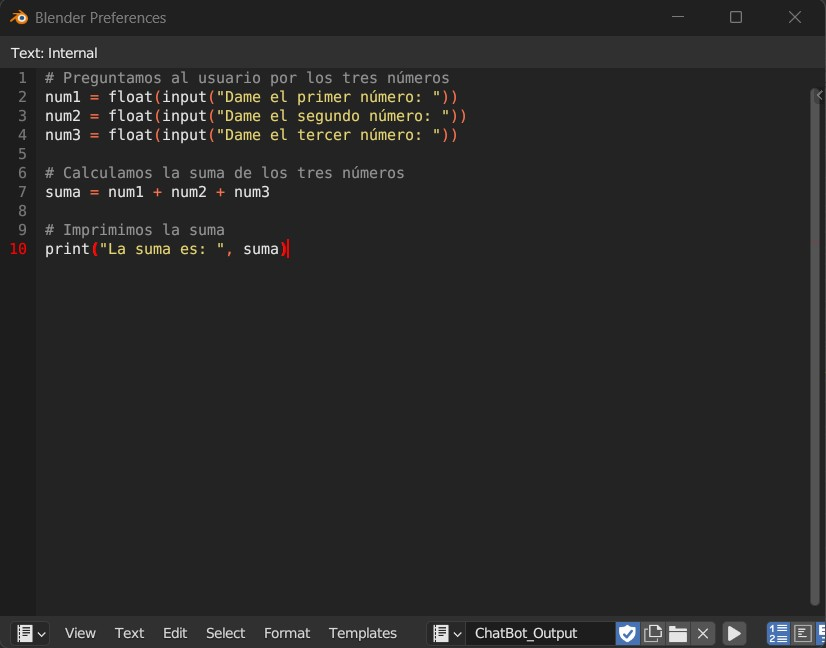
\includegraphics[width=0.8\textwidth]{figs/cu2_2.jpg}
    \caption{Captura de pantalla del código generado en el panel de scripting de Blender para el CU2 en las pruebas funcionales}
    \label{fig:cu2_2}
  \end{figure}

% Imagen
  \begin{figure}[h!tb]
    \centering
    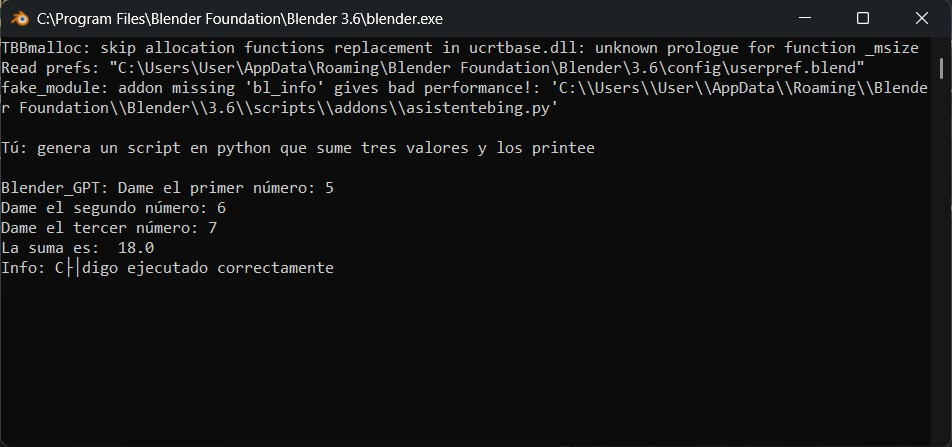
\includegraphics[width=0.8\textwidth]{figs/cu2_3.jpg}
    \caption{Captura de pantalla del código ejecutado en el terminal de Blender para el CU2 en las pruebas funcionales}
    \label{fig:cu2_3}
  \end{figure}

% Imagen
  \begin{figure}[h!tb]
    \centering
    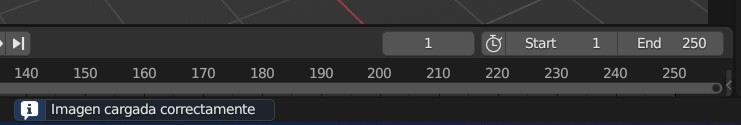
\includegraphics[width=0.8\textwidth]{figs/cu3.jpg}
    \caption{Captura de pantalla de la barra de notificaciones de blender para el CU3 en las pruebas funcionales}
    \label{fig:cu3}
  \end{figure}

% Imagen
  \begin{figure}[h!tb]
    \centering
    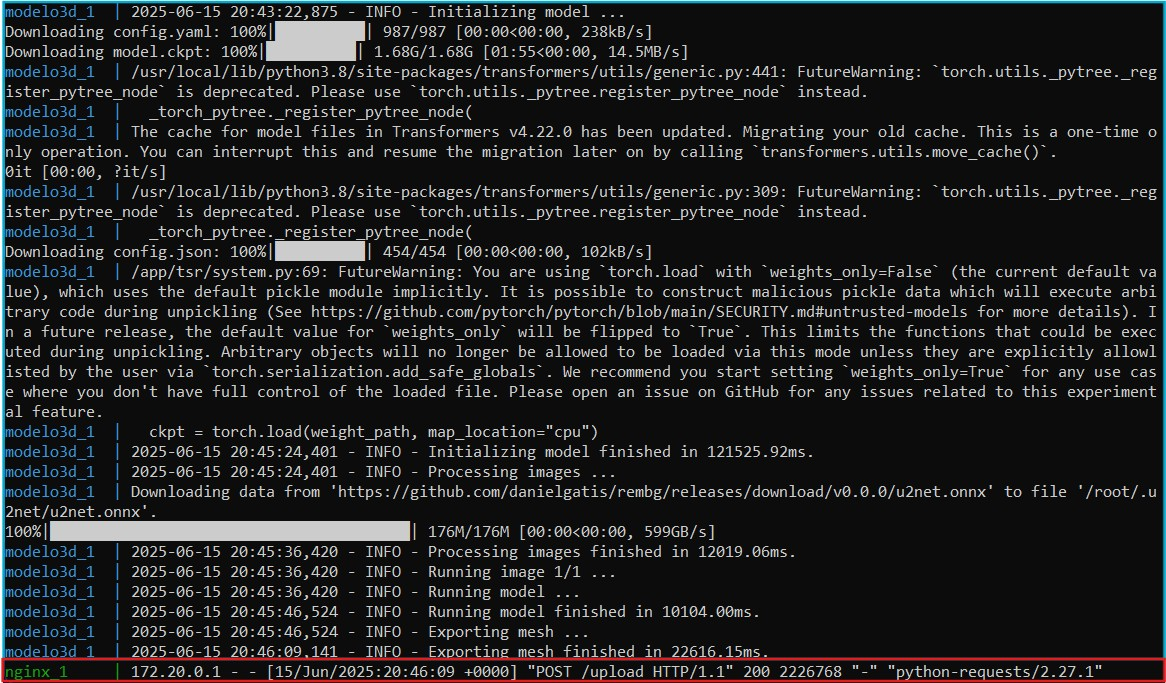
\includegraphics[width=0.8\textwidth]{figs/cu4cu9.jpg}
    \caption{Captura de pantalla del terminal de logs del servidor para el CU4 y CU9 en las pruebas funcionales}
    \label{fig:cu4cu9}
  \end{figure}

% Imagen
  \begin{figure}[h!tb]
    \centering
    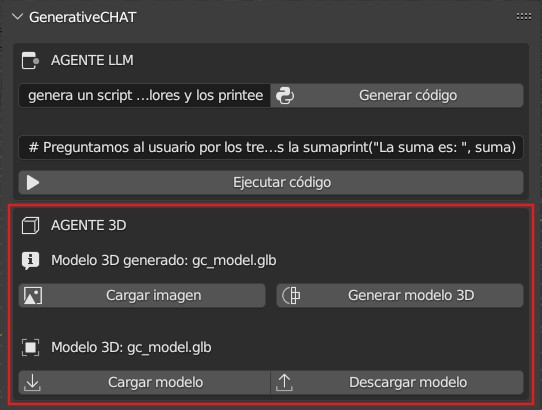
\includegraphics[width=0.8\textwidth]{figs/cu5_1.jpg}
    \caption{Captura de pantalla del add-on con el modelo 3D generado para el CU5 en las pruebas funcionales}
    \label{fig:cu5_1}
  \end{figure}

% Imagen
  \begin{figure}[h!tb]
    \centering
    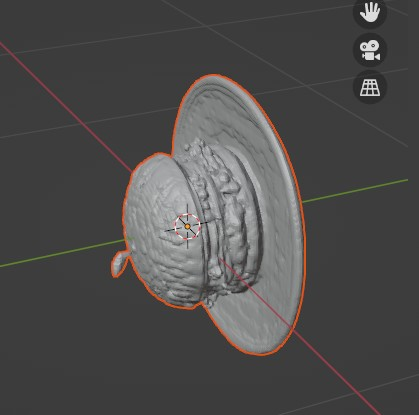
\includegraphics[width=0.8\textwidth]{figs/cu5_2.jpg}
    \caption{Captura de pantalla del modelo 3D cargado en la escena de Blender para el CU5 en las pruebas funcionales}
    \label{fig:cu5_2}
  \end{figure}

% Imagen
  \begin{figure}[h!tb]
    \centering
    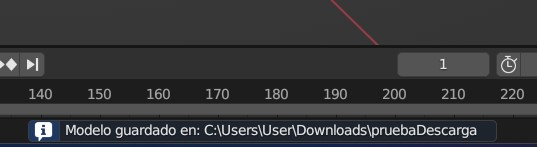
\includegraphics[width=0.8\textwidth]{figs/cu6_1.jpg}
    \caption{Captura de pantalla de la barra de notificaciones de blender para el CU6 en las pruebas funcionales}
    \label{fig:cu6_1}
  \end{figure}

% Imagen
  \begin{figure}[h!tb]
    \centering
    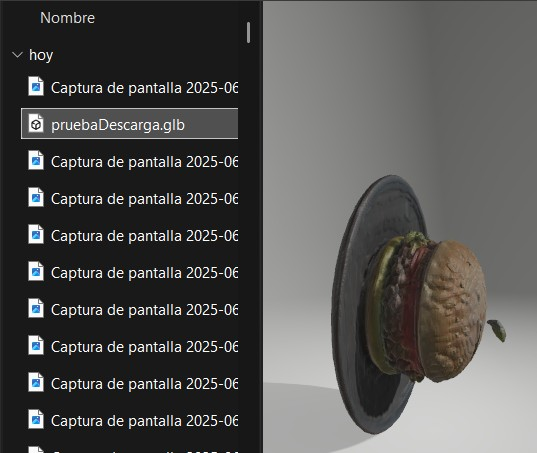
\includegraphics[width=0.8\textwidth]{figs/cu6_2.jpg}
    \caption{Captura de pantalla de la carpeta de descargas con el modelo 3D exportado para el CU6 en las pruebas funcionales}
    \label{fig:cu6_2}
  \end{figure}

% Imagen
  \begin{figure}[h!tb]
    \centering
    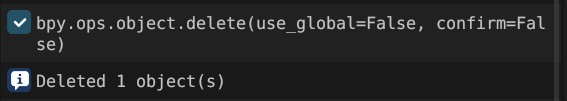
\includegraphics[width=0.8\textwidth]{figs/cu7.jpg}
    \caption{Captura de pantalla del terminal de blender despues de revertir la eliminación de un objeto para el CU7 en las pruebas funcionales}
    \label{fig:cu7}
  \end{figure}


\clearpage
\section{Resultados de las pruebas de rendimiento}
\label{sec:puntoC2}

% Imagen R1
  \begin{figure}[h!tb]
    \centering
    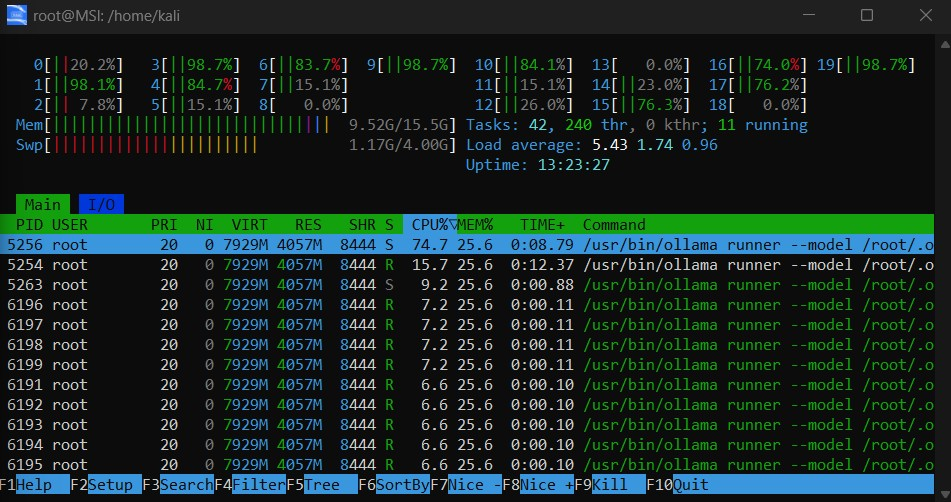
\includegraphics[width=0.8\textwidth]{figs/LLM1.jpg}
    \caption{Resultado de la prueba de rendimiento con 1 petición sobre el microservicio del modelo LLM}
    \label{fig:resRend1LLM}
  \end{figure}

% Imagen R5
  \begin{figure}[h!tb]
    \centering
    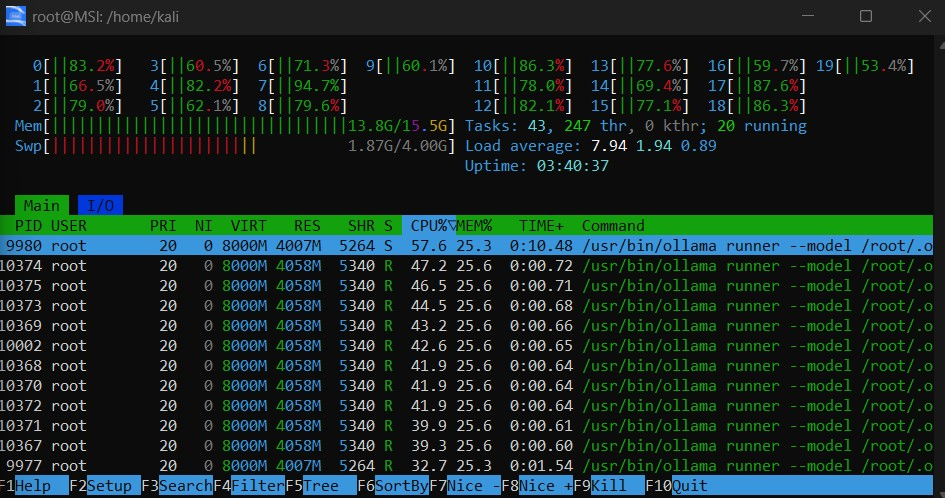
\includegraphics[width=0.8\textwidth]{figs/LLM2.jpg}
    \caption{Resultado de la prueba de rendimiento con 2 petición sobre el microservicio del modelo LLM}
    \label{fig:resRend2LLM}
  \end{figure}

% Imagen R6
  \begin{figure}[h!tb]
    \centering
    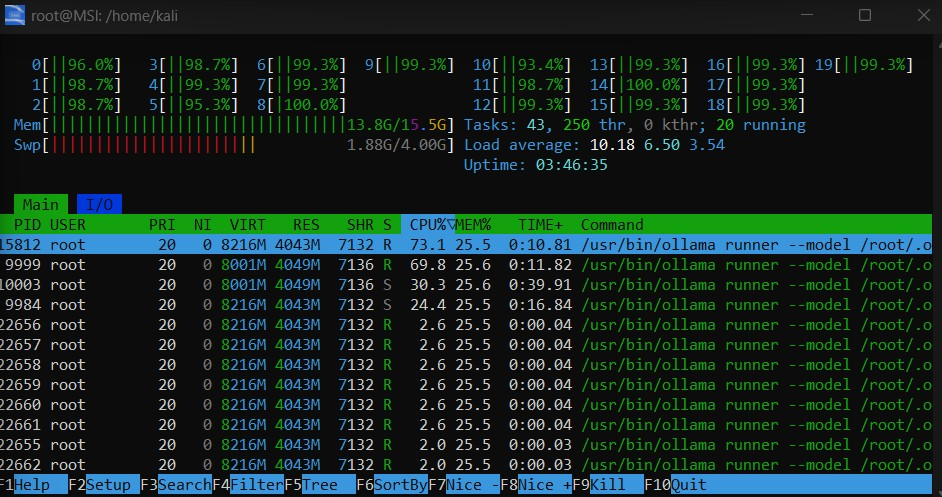
\includegraphics[width=0.8\textwidth]{figs/LLM3.jpg}
    \caption{Resultado de la prueba de rendimiento con 3 petición sobre el microservicio del modelo LLM}
    \label{fig:resRend3LLM}
  \end{figure}

% Imagen R2
  \begin{figure}[h!tb]
    \centering
    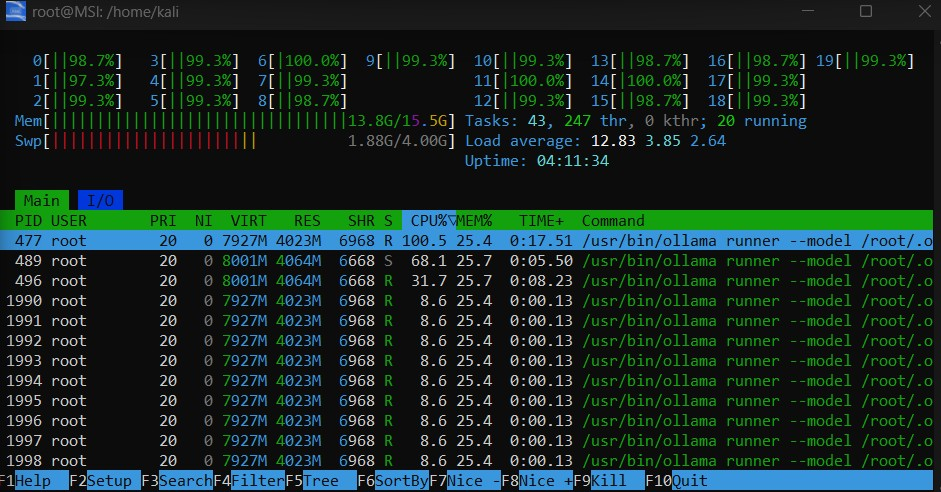
\includegraphics[width=0.8\textwidth]{figs/LLM4.jpg}
    \caption{Resultado de la prueba de rendimiento con 4 petición sobre el microservicio del modelo LLM}
    \label{fig:resRend4LLM}
  \end{figure}

% Imagen R3
  \begin{figure}[h!tb]
    \centering
    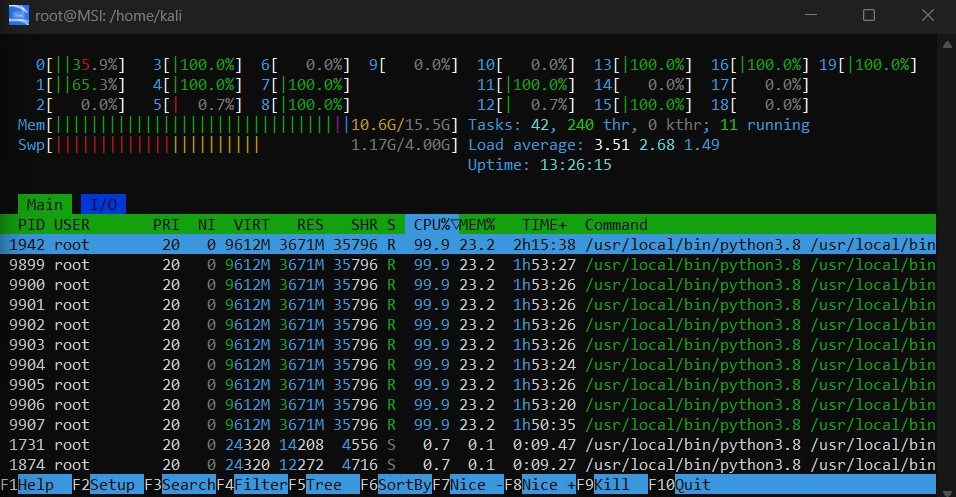
\includegraphics[width=0.8\textwidth]{figs/3D1.jpg}
    \caption{Resultado de la prueba de rendimiento con 1 petición sobre el microservicio del modelo 3D TripoSR}
    \label{fig:resRend13D}
  \end{figure}

% Imagen R7
  \begin{figure}[h!tb]
    \centering
    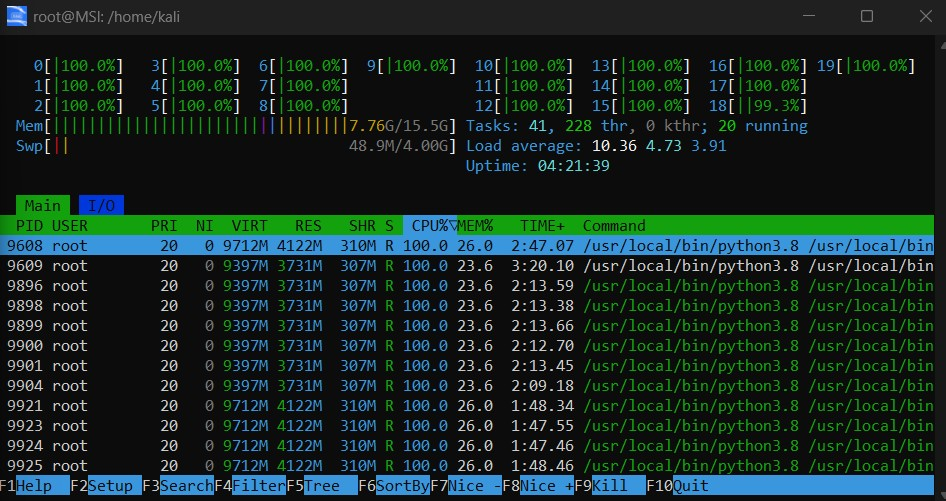
\includegraphics[width=0.8\textwidth]{figs/3D2.jpg}
    \caption{Resultado de la prueba de rendimiento con 2 petición sobre el microservicio del modelo 3D TripoSR}
    \label{fig:resRend23D}
  \end{figure}

% Imagen R8
  \begin{figure}[h!tb]
    \centering
    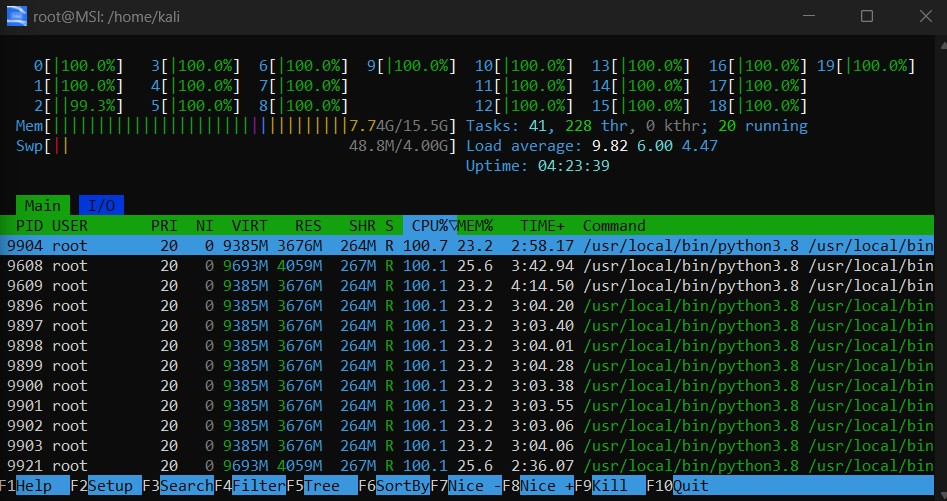
\includegraphics[width=0.8\textwidth]{figs/3D3.jpg}
    \caption{Resultado de la prueba de rendimiento con 3 petición sobre el microservicio del modelo 3D TripoSR}
    \label{fig:resRend33D}
  \end{figure}

% Imagen R4
  \begin{figure}[h!tb]
    \centering
    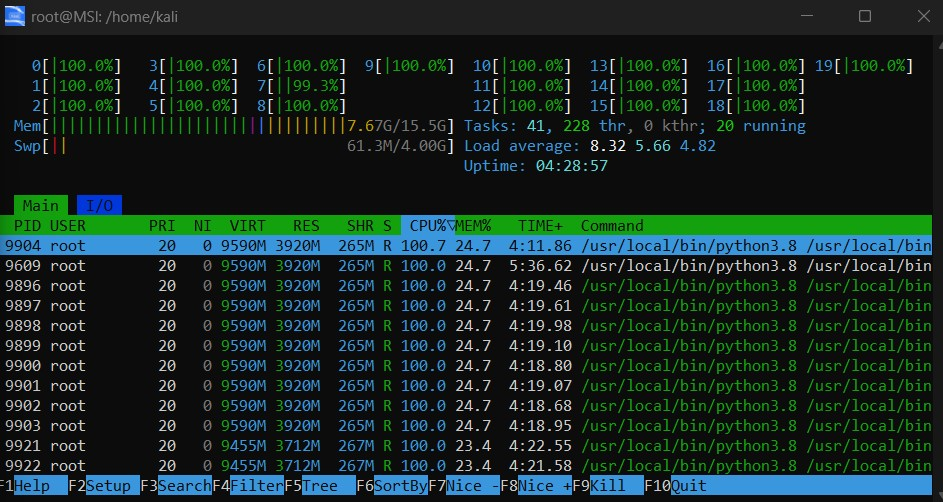
\includegraphics[width=0.8\textwidth]{figs/3D4.jpg}
    \caption{Resultado de la prueba de rendimiento con 4 petición sobre el microservicio del modelo 3D TripoSR}
    \label{fig:resRend43D}
  \end{figure}


\end{document}

%%% Local Variables:
%%% mode: latex
%%% TeX-master: t
%%% End:
